% Consolidated single manuscript: prediction, impact analysis, and
% mitigation in one document (technical paper + prediction companion merged,
% September 2026). Figures reuse the pipeline's own chart files
% (figures/figure_*.png, figures/supplemental/s*.png) plus exhibits generated
% from the same tables (figures/pred_*.png); all tables transcribe the
% September 2026 pipeline run (tables/table_*.csv, tables/pred_*.csv) rounded
% for readability --- see the pipeline's Table 8.6 for provenance.
% Compile from article/: pdflatex this file twice.
\documentclass[11pt,a4paper]{article}
\usepackage[margin=1in]{geometry}
\usepackage{amsmath,amssymb,booktabs,array,graphicx,xurl,hyperref}
\usepackage[table]{xcolor}
\usepackage{natbib}
\usepackage[section]{placeins}
\usepackage{enumitem}
\usepackage[font=small,labelfont=bf,labelsep=period,justification=raggedright,singlelinecheck=false]{caption}
\hypersetup{colorlinks=true,linkcolor=blue,citecolor=blue,urlcolor=blue,
pdftitle={Circular Capital in the Artificial Intelligence Stack: A Game-Theoretic Analysis of Market Power, Financial Fragility, and Welfare},
pdfauthor={}}
\setcitestyle{authoryear,round}
\setlength{\bibhang}{0.5in}
\graphicspath{{../figures/}}
% Pipeline-fed values: Table 8.7 intervals render from code output
% (generated_a8_intervals.tex, rewritten every ai_ecosystem_model run).
% GENERATED by StructuralEstimationAnalyzer.write_tex_macros -- do not edit.
% Values render Table 8.7 (table_8.7_structural_estimation.csv);
% the ai_ecosystem_model stage rewrites this file every run.
\newcommand{\AeightCapex}{[0.35, 2.63]}
\newcommand{\AeightHhi}{[0.10, 1.67]}
\newcommand{\AeightCirc}{[0.74, 3.00$+$]}
\newcommand{\AeightExub}{[0.00$+$, 1.04]}

\setlength{\parskip}{0.5em}
\rowcolors{2}{gray!10}{white}
% Whitespace control: many large floats share pages with text, so tighten
% float spacing and let top/bottom areas fill more aggressively.
\setlength{\textfloatsep}{12pt plus 2pt minus 2pt}
\setlength{\abovecaptionskip}{6pt}
\renewcommand{\textfraction}{0.07}
\renewcommand{\topfraction}{0.93}
\renewcommand{\bottomfraction}{0.9}
\setcounter{topnumber}{3}
\setcounter{bottomnumber}{3}
\title{Circular Capital in the Artificial Intelligence Stack:
A Game-Theoretic Analysis of Market Power, Financial Fragility, and Welfare}
\author{}
\date{}
\begin{document}
\maketitle
\begin{abstract}
\noindent The 2024--2026 artificial-intelligence investment boom exhibits the
financing structure that preceded previous round-trip busts: dense,
committed circular capital in which upstream investment returns
downstream as contracted compute spend, measured here at \$675.40~billion
across 17 committed contracts. This architecture concentrates burst
incidence upstream. While bubble indicators peak at $\sim$83\% among
frontier labs where valuations have detached from revenue, credit
markets already price stack leverage through a record single-name CDS
spread (215 bp) and downgrade. Six solved bilateral games reveal an
aggregate deadweight loss of \$416.77~billion (71.28\% efficiency),
with non-cooperation binding in the Hardware--Cloud bottleneck.
Consequently, a severe repricing destroys $\sim$\$239~billion of Hardware
and $\sim$\$133~billion of Cloud value first, transmitting a $\sim$\$139~billion
loss ($\sim$0.45\% of GDP) to the U.S. economy via capex and
wealth channels. This loss hierarchy is structural: it survives 16
parameter extremes and 300 joint Monte Carlo draws, and reproduces the
historical loss order when applied blind to 2006--07 pre-crisis inputs from
the 2008 Global Financial Crisis. By benefit--cost ratio, optimal policy sequencing prioritizes
contract disclosure and lending caps. Three empirical
triggers would cancel the forecast if observed.
\medskip

\noindent\textbf{Keywords:} artificial intelligence; financial bubbles;
circular dealing; vendor financing; game theory; burst prediction;
financial stability; competition policy.
\medskip

\noindent\textbf{JEL codes:} D43, G01, G12, G14, L13, L41, E44, O33.
\end{abstract}
% FEM-2026 portal rule: page 1 carries only the title + abstract; TOC opens on p2.
\newpage
% Set the TOC small with no paragraph gaps: 23 sections spill a near-empty
% page at full size (every entry pays \parskip).
\begingroup
\setlength{\parskip}{0pt}
\small\tableofcontents
\endgroup
\newpage

\section{Introduction}
This paper converts a measured financing structure into a dated,
testable prediction: an AI-asset repricing is likely while the current
committed spend cycle runs; its losses will land first on Hardware, then
Cloud, then frontier labs, then apps; and the severe case costs the US
economy roughly \$100--150~billion. Section~\ref{sec:prediction} states
that forecast as eight numbered claims, each with an assessed likelihood
(or an explicit abstention, P8) and a pointer to the observable that would
overturn it. The remaining
sections supply the evidence (Sections~\ref{sec:capital}--\ref{sec:contagion}),
the record of stress testing and historical validation
(Sections~\ref{sec:robustness}--\ref{sec:backtest}), and the investment and
policy implications (Sections~\ref{sec:triggers}--\ref{sec:policy}).
An Online Appendix documents the grading apparatus, assumptions, and
caveats; the body below advances the predictions without interruption.

The argument is a single chain with five links. \textbf{Measurement:}
\$675.40~billion of committed circular capital is read off signed
contracts, not inferred from sentiment or multiples
(Section~\ref{sec:capital}). \textbf{Mechanism:} six solved bilateral games
show non-cooperation binds in exactly one cell --- Hardware versus Cloud ---
trapping value upstream (Sections~\ref{sec:games}--\ref{sec:core}).
\textbf{Incidence:} the trap fixes the burst order --- Hardware (the
Toolmakers), Cloud (the Landlords), frontier labs (the Brain Builders),
apps (the App Builders) --- with formation conditions worst where private marks
have detached furthest (Sections~\ref{sec:bubble}--\ref{sec:burst}).
\textbf{Validation:} the order survives sixteen extremes and 300 joint
draws; the same modules recover the 2008 loss order, and on telecom
equipment in 2001 they recover the mechanism --- the stuck vendor cell,
the first-to-fail ranking, the formation order --- while missing dollar
incidence, which multiple compression decides outside contract arithmetic
(Sections~\ref{sec:robustness}--\ref{sec:backtest}). \textbf{Action:}
triggers monitor the preconditions and remedies sequence by benefit--cost
ratio, disclosure and lending caps first
(Sections~\ref{sec:triggers}--\ref{sec:policy}). Break any link and the
conclusion falls; Section~\ref{sec:validation} names the observables
that would break each one. One distinction governs every number that
follows: \emph{rankings} are the high-confidence claims; \emph{dollar
figures} mark scenario scale for sizing remedies.

\section{Central Forecast: Repricing Likelihood, Loss Incidence, and Macroeconomic Cost}\label{sec:prediction}
This paper makes a prediction with three parts. \textbf{First}, an AI-asset
repricing is likely while the current committed spend cycle runs: the
conditions that have preceded every modern round-trip bust --- dense
reciprocal financing, private marks detached from capturable revenue, and
credit markets starting to charge for leverage --- are all present at once.
\textbf{Second}, the damage has a fixed address: Hardware first
($\sim$\$239B), Cloud second ($\sim$\$133B), frontier labs third
($\sim$\$85B), app companies last ($\sim$\$21B), because contracts, not
sentiment, decide where losses land. \textbf{Third}, the US GDP cost of the
severe case is $\sim$\$139B ($\sim$0.45\%), composed of canceled tech
investment ($\sim$\$120B) plus the wealth effect of falling equities
($\sim$\$19B).

What this paper does \emph{not} predict is a date. Timing belongs to funding
rounds, credit events, and capex guidance --- the triggers of Section~\ref{sec:triggers} ---
not to models. Everything else here is a measured claim, not a scenario
sketch: the capital structure is read off contracts, the binding constraint
is proved in solved games, and the resulting incidence ranking is the same
order that survives every stress battery and transfers to 2008. The result
is a standing warning with an address book: it tells you what breaks, in
what order, at roughly what scale, and what to do before it happens.

\emph{How seriously to take each claim.} Every numbered prediction below
carries two separate tags. \textbf{Likelihood} is the author's assessed
probability that the claim proves right, on the fixed scale in
Table~\ref{tab:likelihood-scale} --- a judgment in the forecasting tradition
(IPCC, Tetlock), not a model estimate. \textbf{Confidence} rates the quality
of the evidence behind that judgment (High = contracts plus surviving stress
tests; Medium = scenario arithmetic that moves with inputs; Low = no
evidentiary basis). Model vote-shares (16/16, 100\%, 65\%) measure
\emph{robustness}, and formation scores (82.9\% etc.)\ measure
\emph{vulnerability} --- neither is the probability of the event. The two
numbers that look most like probabilities in this paper are therefore the
two you must not mistake for forecasts; the actual event probabilities are
the author's, stated in the registry.

\begin{table}[htbp]
\centering
\caption{Likelihood scale for author-assessed probabilities. Used only in the registry below; nowhere else in the paper does a percent sign denote an event probability.}
\label{tab:likelihood-scale}
\begin{tabular}{lc}
\toprule
Wording & Assessed probability \\
\midrule
Very likely & 85--95\% \\
Likely & 65--80\% \\
More likely than not & 50--65\% \\
Toss-up & $\sim$50\% \\
Unlikely & below 35\% \\
\bottomrule
\end{tabular}
\end{table}

\begin{table}[htbp]
\centering
\caption{Prediction registry: every claim, its likelihood, its evidence grade, and what retires it.}
\label{tab:registry}
\begin{tabular}{l>{\raggedright\arraybackslash}p{4.4cm}>{\raggedright\arraybackslash}p{2.7cm}c>{\raggedright\arraybackslash}p{3.0cm}}
\toprule
ID & Claim & Likelihood & Confidence & Overturned by \\
\midrule
P1 & AI-asset repricing before the committed spend cycle exhausts itself & Likely ($\sim$65\%) & Medium & Validation tests 1--2 \\
P2 & \emph{Conditional on a severe burst,} losses rank Hardware $>$ Cloud $>$ labs $>$ apps & Very likely ($\sim$90\%) & High & Test 3 (ranking flips) \\
P3 & Severe GDP cost lands near \$100--150B ($\sim$0.3--0.5\%), mostly via canceled capex & More likely than not ($\sim$55\%) & Medium & A burst with no capex cut \\
P4 & Frontier-lab funding stress is the nearest trigger & Likely ($\sim$70\%) & Medium & A first break elsewhere (Sec.~\ref{sec:triggers}) \\
P5 & Labs carry the highest bubble vulnerability (formation rank FM first) & More likely than not ($\sim$60\%) & Medium & Formation rank flips (65\% joint agreement) \\
P6 & Round two is small ($\sim$\$15B), mostly on labs ($\sim$\$13.9B of $\sim$\$15.2B) & More likely than not ($\sim$60\%) & Medium & Collateral fire sale (Sec.~\ref{sec:contagion}) \\
P7 & Disclosure first, lending caps second is the optimal remedy sequence (caps still rank first by BCR) & Likely ($\sim$70\%) & Medium & BCR rank reversal (Sec.~\ref{sec:policy}) \\
P8 & Any calendar date for the repricing & --- (unassigned) & Low & --- (no date predicted) \\
\bottomrule
\end{tabular}
\end{table}

P8 stays unassigned by design: structural game theory identifies equilibrium
fragility and loss topology, while the tipping date depends on
non-deterministic catalytic triggers (funding-round failures, credit
repricing).

Read P2 the way it is written: \emph{conditional.} The paper assigns no
probability to a severe burst occurring at all (that is P1's job, at
$\sim$65\%); it assigns $\sim$90\% to the ranking \emph{given} that one
occurs. Multiplying them, the joint statement ``a severe burst with
Hardware first'' sits near 60\% --- which is why the headline phrase is
``a standing warning with an address book,'' not ``a forecast.'' Dollar
levels throughout are scenario markers: P3's wide band (\$100--150B) is the
honest width; the Online Appendix documents what each tag rests on.

\begin{figure}[htbp]
\centering
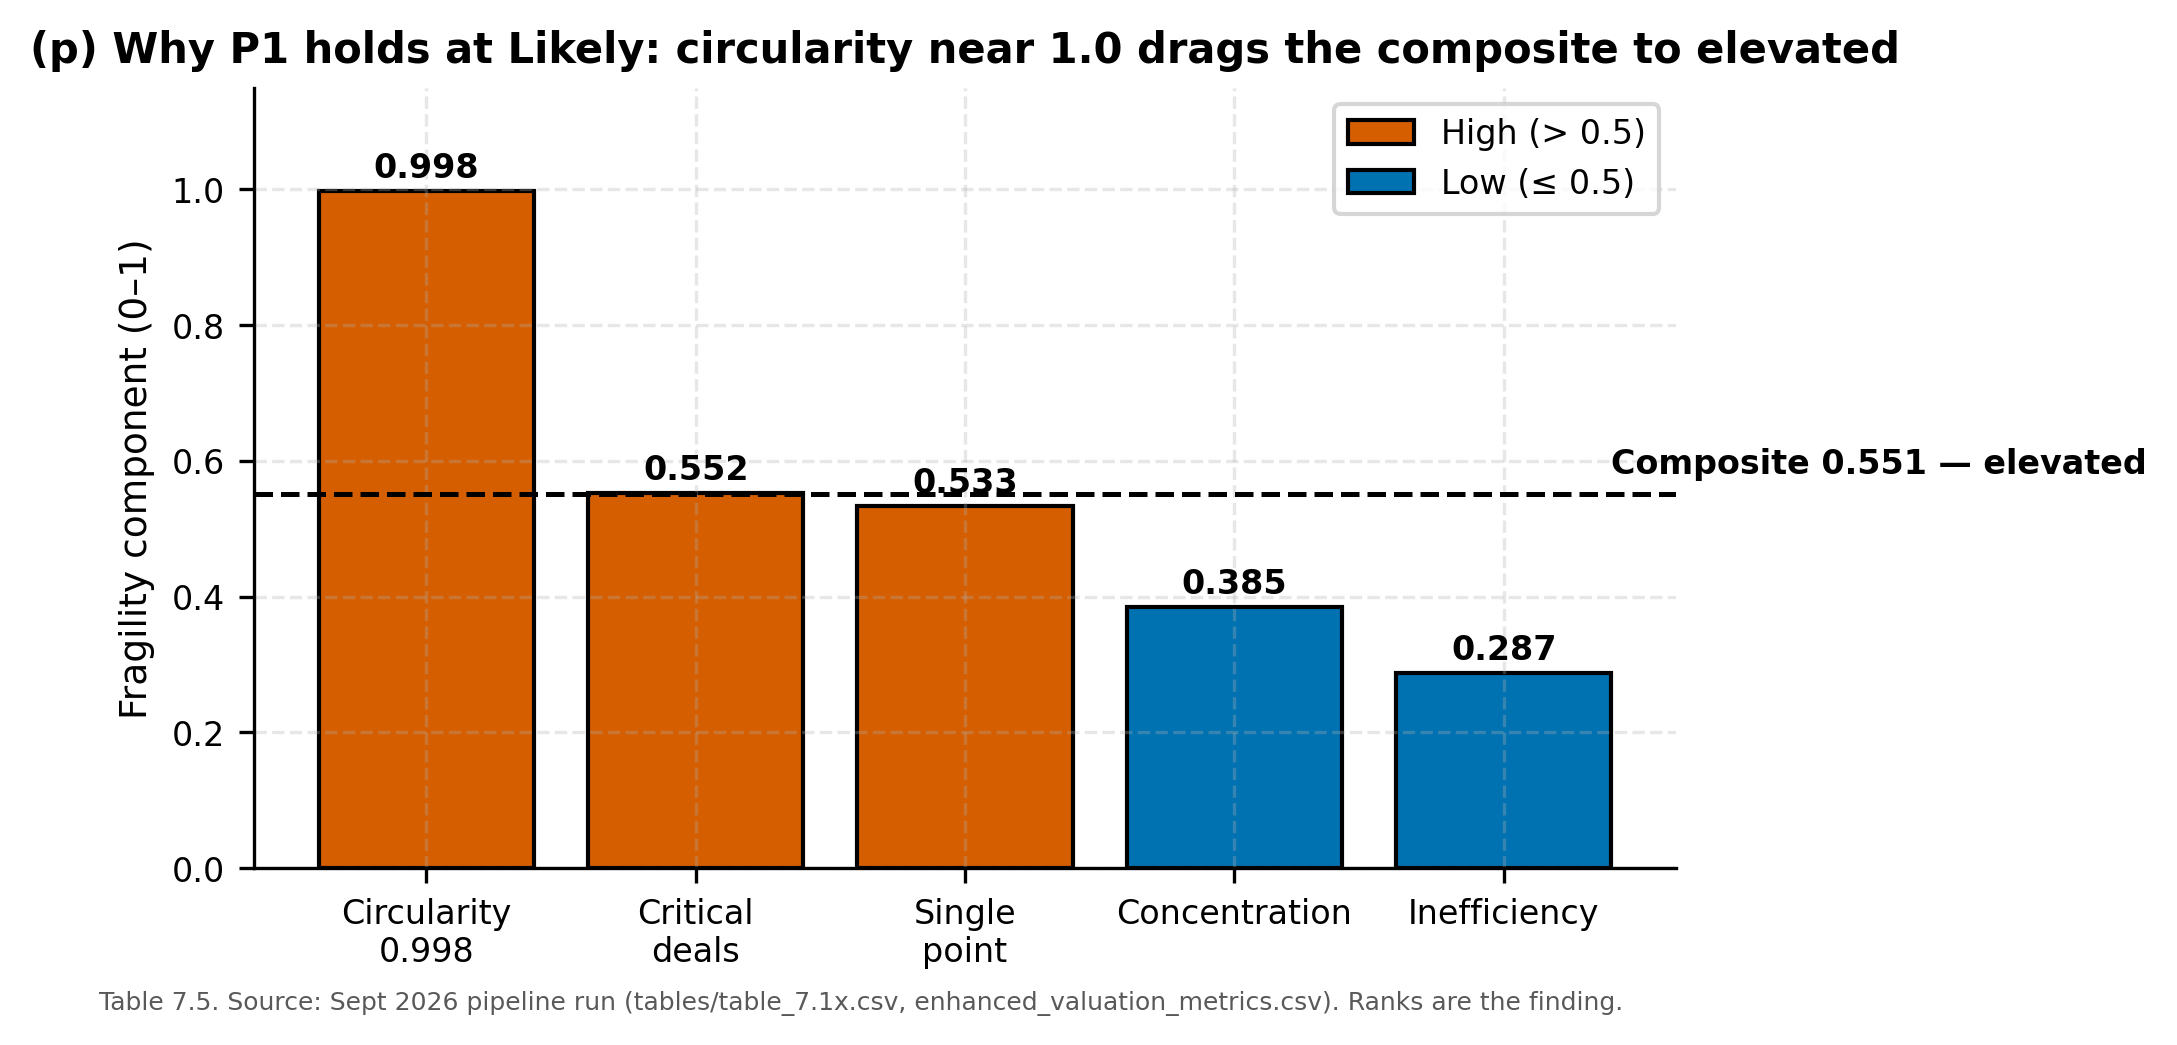
\includegraphics[width=\textwidth,height=0.82\textheight,keepaspectratio]{pred_fragility.png}
\caption{System fragility at a glance (Table~7.5): circularity scores 0.998 of 1.0 --- the stack is almost perfectly round-tripped --- dragging the composite to 0.551, band ``elevated.'' This single chart is the visual evidence behind P1's Likely grade.}
    \label{fig:01-system-fragility-at-a}
\end{figure}

\section{Analytical Approach: Contractual Exposure as the Forecasting Primitive}\label{sec:foundation}
Most bubble calls argue about prices. This one argues about \emph{plumbing}:
the \$675.40B of committed round-trip financing, across 17 booked deals,
that wires the AI stack into a single fate-sharing machine. When company A
invests in company B and B contractually spends the money back at A, two
balance sheets become one balance sheet wearing two logos. Prices can then
stay high for good reasons (real revenues: NVIDIA's record \$57.0B quarter, Q3 FY2026)
while the financing underneath stays fragile. That split --- real revenues,
fragile financing --- is what makes a burst prediction possible without a
price prediction: you do not need to know when enthusiasm fades, only where
the contracts point when it does. The machinery is a single Python
pipeline of 35 classes covering data validation, market structure, solved
games, welfare accounting, bubble diagnostics, and valuation, gated end to
end by 364 tests.

Why this toolkit and not price charts. Traditional bubble models study
anonymous markets through prices, sentiment, or aggregates; the AI stack is
the opposite --- a handful of giants negotiating bespoke bilateral
contracts --- so the tools model the plumbing directly. \emph{Game theory}
solves each pairwise negotiation for its stable outcome, exposing the one
gridlocked cell. The \emph{Herfindahl--Hirschman Index} (the DOJ
concentration screen, highly concentrated above 2,500) quantifies the
chokepoint: at 3,851, no diversified fringe exists to absorb a failure.
\emph{Saltelli global sensitivity analysis} (the variance-decomposition
workhorse of physics and climate modeling) then checks which input actually
drives fragility: shared circular capital scores a total-order index of
0.99, confirming the prediction emphasizes the variable the system is most
sensitive to.

The late-1990s telecom bust is the closest precedent: vendors booking
revenue by lending to their own buyers (Nortel, Lucent), receivables failing
together with sales. Today's version runs mostly on cash
flow rather than debt, with a growing debt-financed fringe --- GPU-collateral
borrowing, the \$500B prospective (unbooked, aspirational) facility, Oracle's \$18B single-day
bond (Table~\ref{tab:10-credit-tripwires-september-2026}) --- which is where a 2008-style accelerant would come from.

\section{Literature Review: Bubbles, Platforms, and Fragility}\label{sec:literature}
This prediction does not start from zero. Five strands of published research
supply its tools, its benchmarks, and its warnings; this section states each
in one paragraph, with pointers for readers who want the originals. Full
references sit in the References list, in APA style.

\emph{1. How economists spot bubbles.} The standard statistical toolkit hunts
explosive price paths: \citet{phillips2011} built the SADF test that
date-stamps when exuberance starts and collapses, and
\citet{phillips2015} generalized it to multiple bubbles. The dot-com
precedent --- world-changing technology alongside prices far above eventual
cash flows --- is documented by \citet{ofek2003}, while \citet{greenwood2019}
show such run-ups predictably end in crashes.
Takeaway for this paper: price tests tell you \emph{whether} something looks
explosive; they cannot tell you \emph{where the losses land}. The financing
graph modeled here answers the second question, which is why the two
approaches complement rather than compete.

\emph{2. What AI does to the economy.} \citet{agrawal2018} and
\citet{agrawal2019} founded the economics-of-AI research program; since then,
field evidence has measured real productivity gains from generative AI
\citep{brynjolfsson2025, noy2023}, while \citet{brynjolfsson2021} and the
classic \citet{david1990} remind us that general-purpose technologies pay off
slowly (the productivity J-curve). Macro watchdogs agree the stakes are
systemic: the IMF flags an AI-correction risk to global growth
\citep{imf2026b} and warns big tech is ``starting to leverage up''
\citep{imf2026}, and the BIS puts AI supply-chain funding complexity on its
risk list \citep{bis2026}. Takeaway: the revolution is real \emph{and} the
financing is fragile --- this paper's ``real revenues, fragile financing''
split is the consensus view, quantified.

\emph{3. Why platforms lock customers in.} Cloud bundling follows the
information-goods logic of \citet{shapiro1999} and \citet{bakos2000};
switching costs and network effects are surveyed by \citet{farrell2007};
sunk-cost market structure by \citet{sutton1991}; semiconductor competition
by \citet{scherer1990}. On policy, the Digital Markets Act \citep{eu2022},
the digital-era competition report \citep{cremer2019}, vertical-stack
analysis \citep{hagiu2025}, the antitrust-paradigm literature
\citep{baker2019}, and data-portability economics \citep{kramer2020} shape
the remedy menu, while the FTC documents investment capital bundled with
cloud spend \citep{ftc2025}. Takeaway: lock-in theory predicts exactly the
\$142.62B switching-cost envelope this paper measures --- the oldest
literature here correctly calls the largest waste category. The classic
monopoly-waste benchmark is \citet{harberger1954}, and the reason fixing one
broken margin can backfire elsewhere is \citet{lipsey1956}.

\emph{4. Vendor financing and fire sales.} Round-trip financing has a known
pathology (telecom vendors lending to their own buyers), and the fire-sale
mechanic --- homogeneous collateral worth less together than apart --- is
formalized by \citet{shleifer1992}. The cascade engine in this paper is the
DebtRank method of \citet{battiston2012}. Takeaway: every moving part of the
contagion story is borrowed from established work; the novelty is wiring
them into one stack with measured exposures.

\emph{5. Concentration and hype measurement.} AI markets concentrate through
fixed training costs and size advantages even without misconduct
\citep{korinek2025}. Scale anchors come from the IEA's energy projections
\citep{iea2026}, IDC spending guides \citep{idc2026}, and the PwC data-center
outlook \citep{pwc2026}; GDP and fiscal baselines from the BEA \citep{bea2026}
and CBO \citep{cbo2022}; valuation discipline from Damodaran's risk-premium
data \citep{damodaran2026}. Takeaway: the calibration inputs are
institutional-grade public sources, listed to the row in the pipeline's
110-row register.

\section{Measurement of Circular Capital: Scale and Composition}\label{sec:capital}
Seventeen committed deals, each traced to primary reporting and re-verified
in September 2026, put \$675.40B of circular capital on the books
(\$1,188.33B tracked including two memo rows); the largest rows are a
\$249.20B aggregate GPU-supply exposure and a \$105B NVIDIA credit
guarantee (Table~\ref{tab:01-largest-committed-circular-exposures}).
Parked \emph{outside} the booked total, exactly as they should be:
Google's \$30B conditional tranche, Amazon's \$20B, an NVIDIA tranche of up
to \$10B, decade-horizon reverse spends, the
\$500B six-platform MOU facility (aspiration, not a contract), and the
\$12.93B NVIDIA--Hugging Face acquisition (a purchase price for control,
with no reverse-spend leg).

\begin{table}[htbp]
\centering
\caption{Largest committed circular exposures (\$B). Full 19-row frame in the pipeline's validated deal ledger (pipeline Table~3 series).}
    \label{tab:01-largest-committed-circular-exposures}
\begin{tabular}{lr}
\toprule
Exposure & Committed \\
\midrule
Aggregate GPU-supply exposure & 249.20 \\
NVIDIA \$105B Ohio credit guarantee & 105.00 \\
Lambda + Nscale compute commitment & 80.00 \\
Fluidstack compute & 50.00 \\
SpaceX Colossus & 45.00 \\
AWS cloud agreement (OpenAI) & 38.00 \\
Azure purchase (Anthropic) & 30.00 \\
CoreWeave contract (Meta) & 14.20 \\
Microsoft--OpenAI / Amazon--Anthropic & 13.00 each \\
\midrule
\textbf{Committed total (17 edges)} & \textbf{675.40} \\
Tracked total (19 rows) & 1,188.33 \\
\bottomrule
\end{tabular}
\end{table}

\begin{figure}[htbp]
\centering
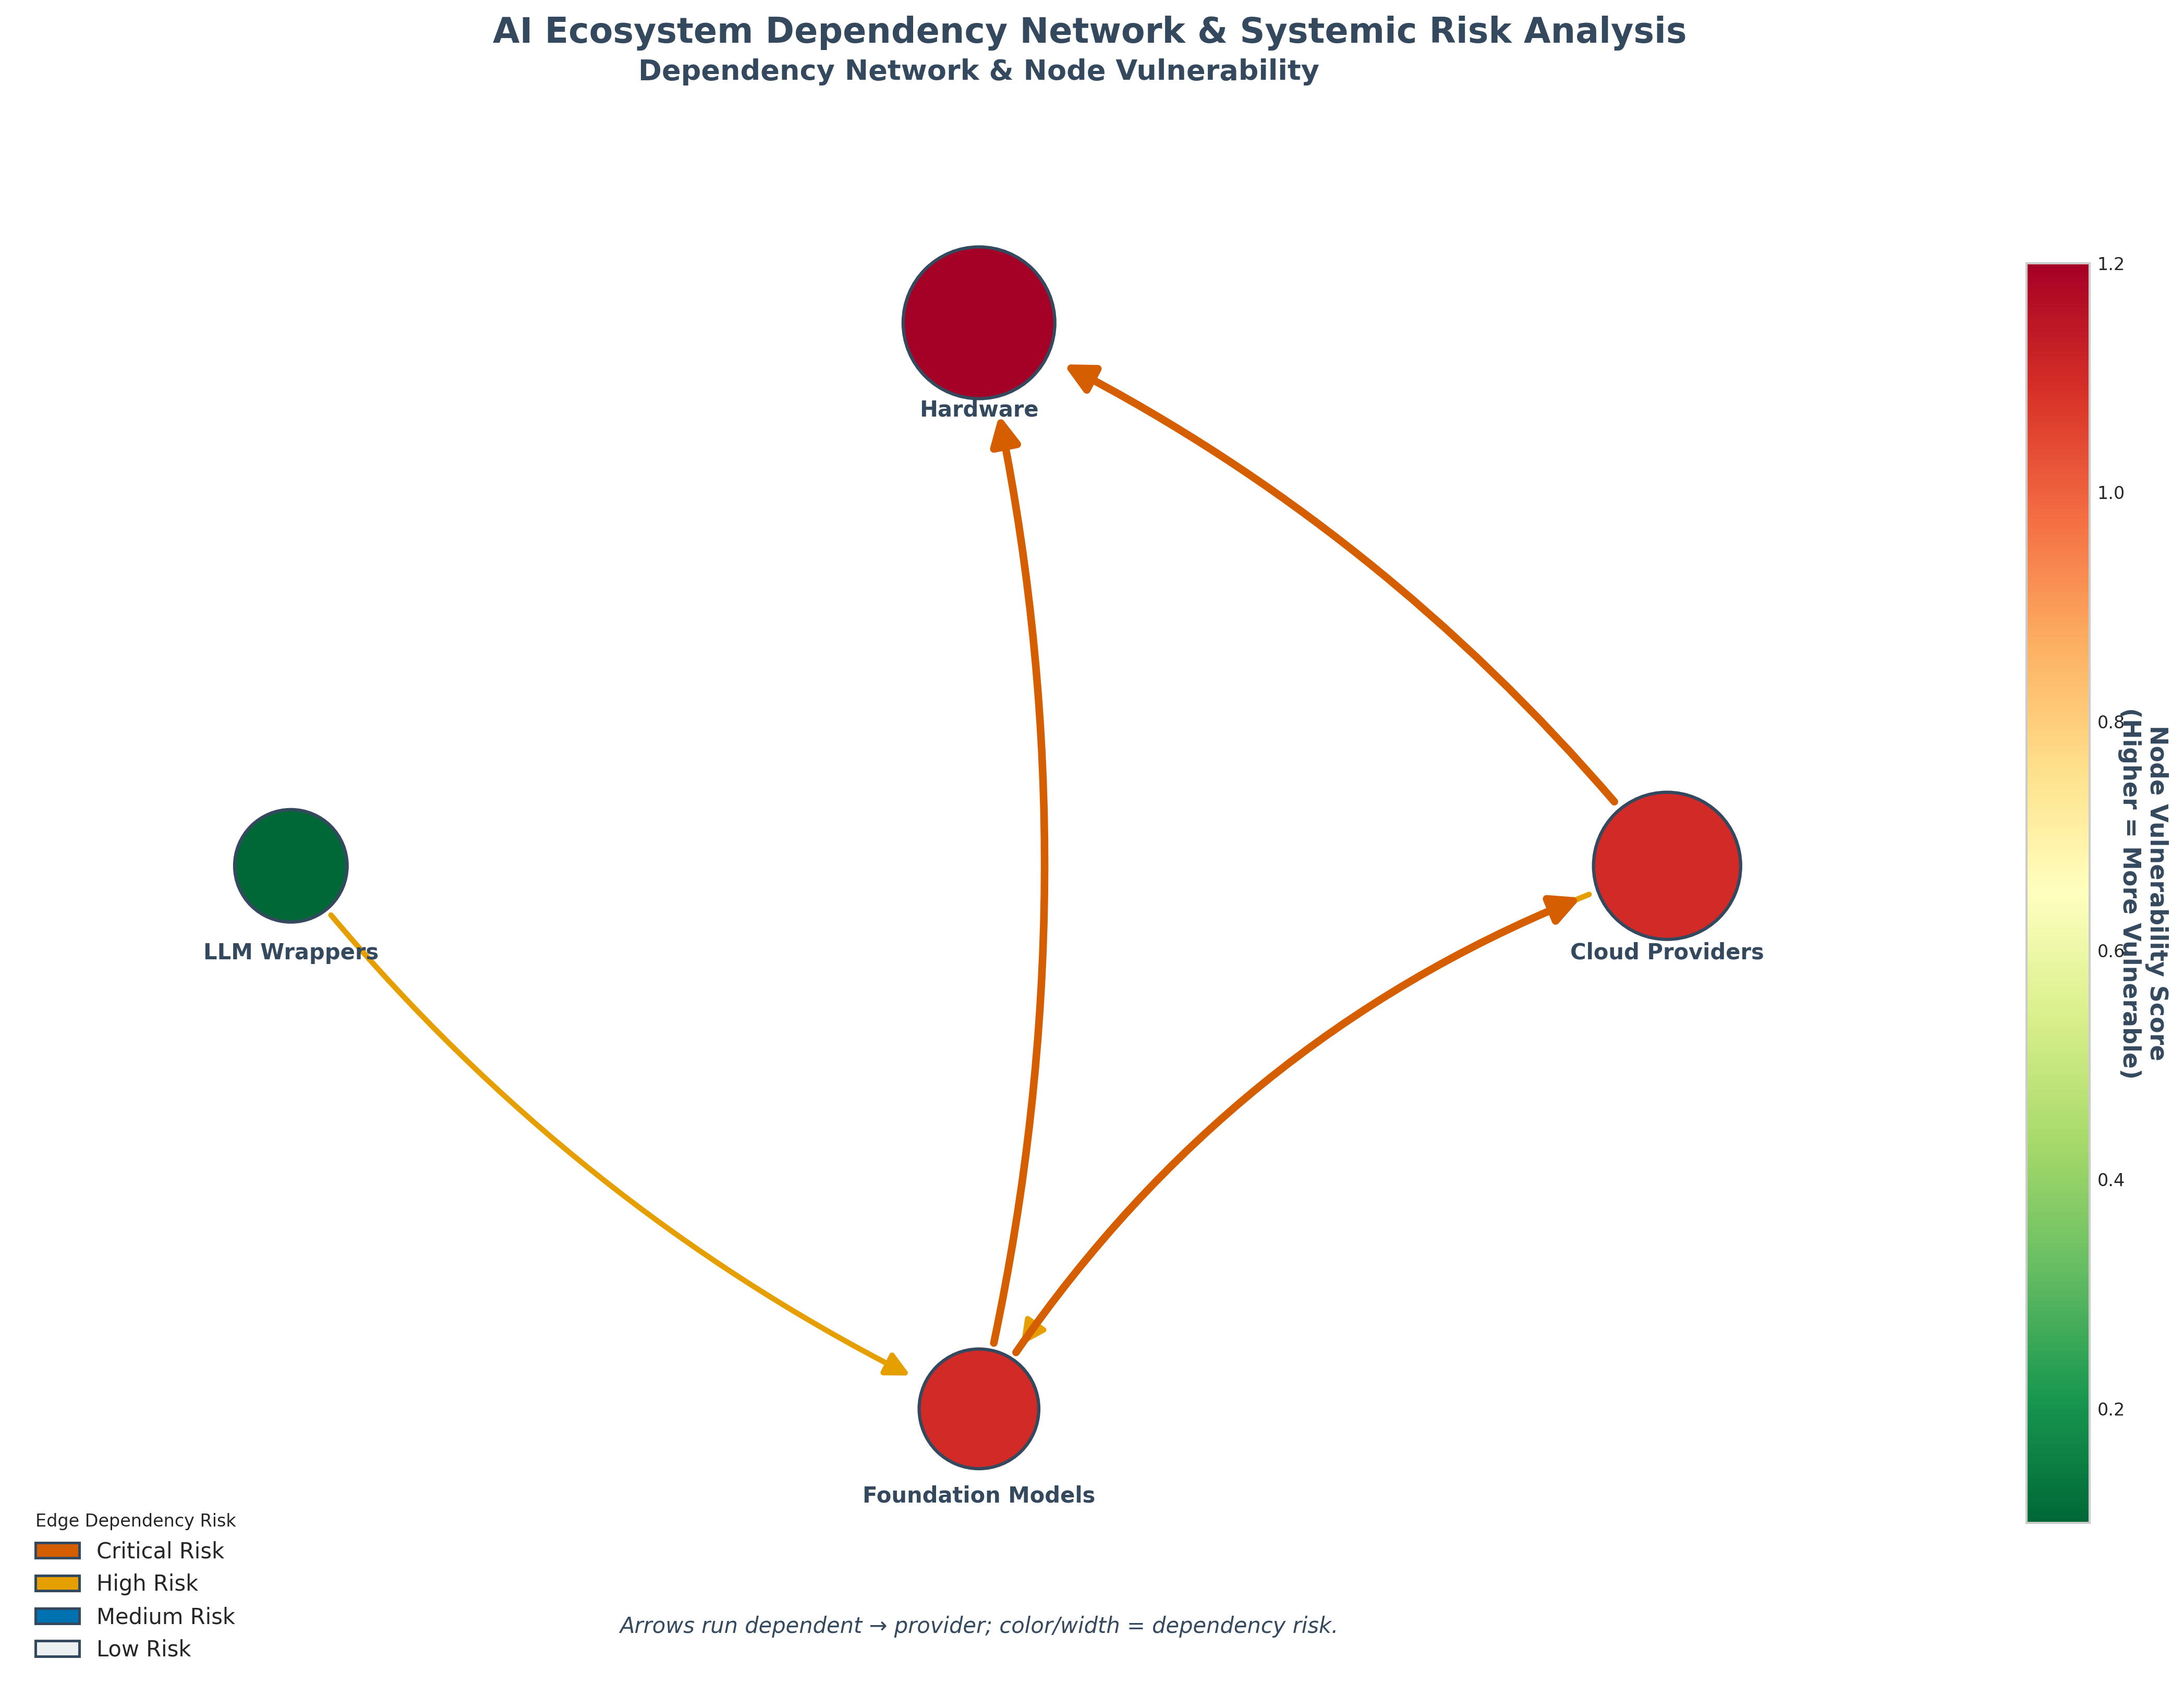
\includegraphics[width=0.8\textwidth,height=0.82\textheight,keepaspectratio]{figure_14.png}
\caption{The fate-sharing machine: directed circular-financing edges and node vulnerability. Foundation Models sit at the receiving end of most circular financing; Hardware anchors the supply side --- which is why the burst ranking runs opposite to the hype.}
    \label{fig:01-the-fatesharing-machine-directed}
\end{figure}

\begin{figure}[htbp]
\centering
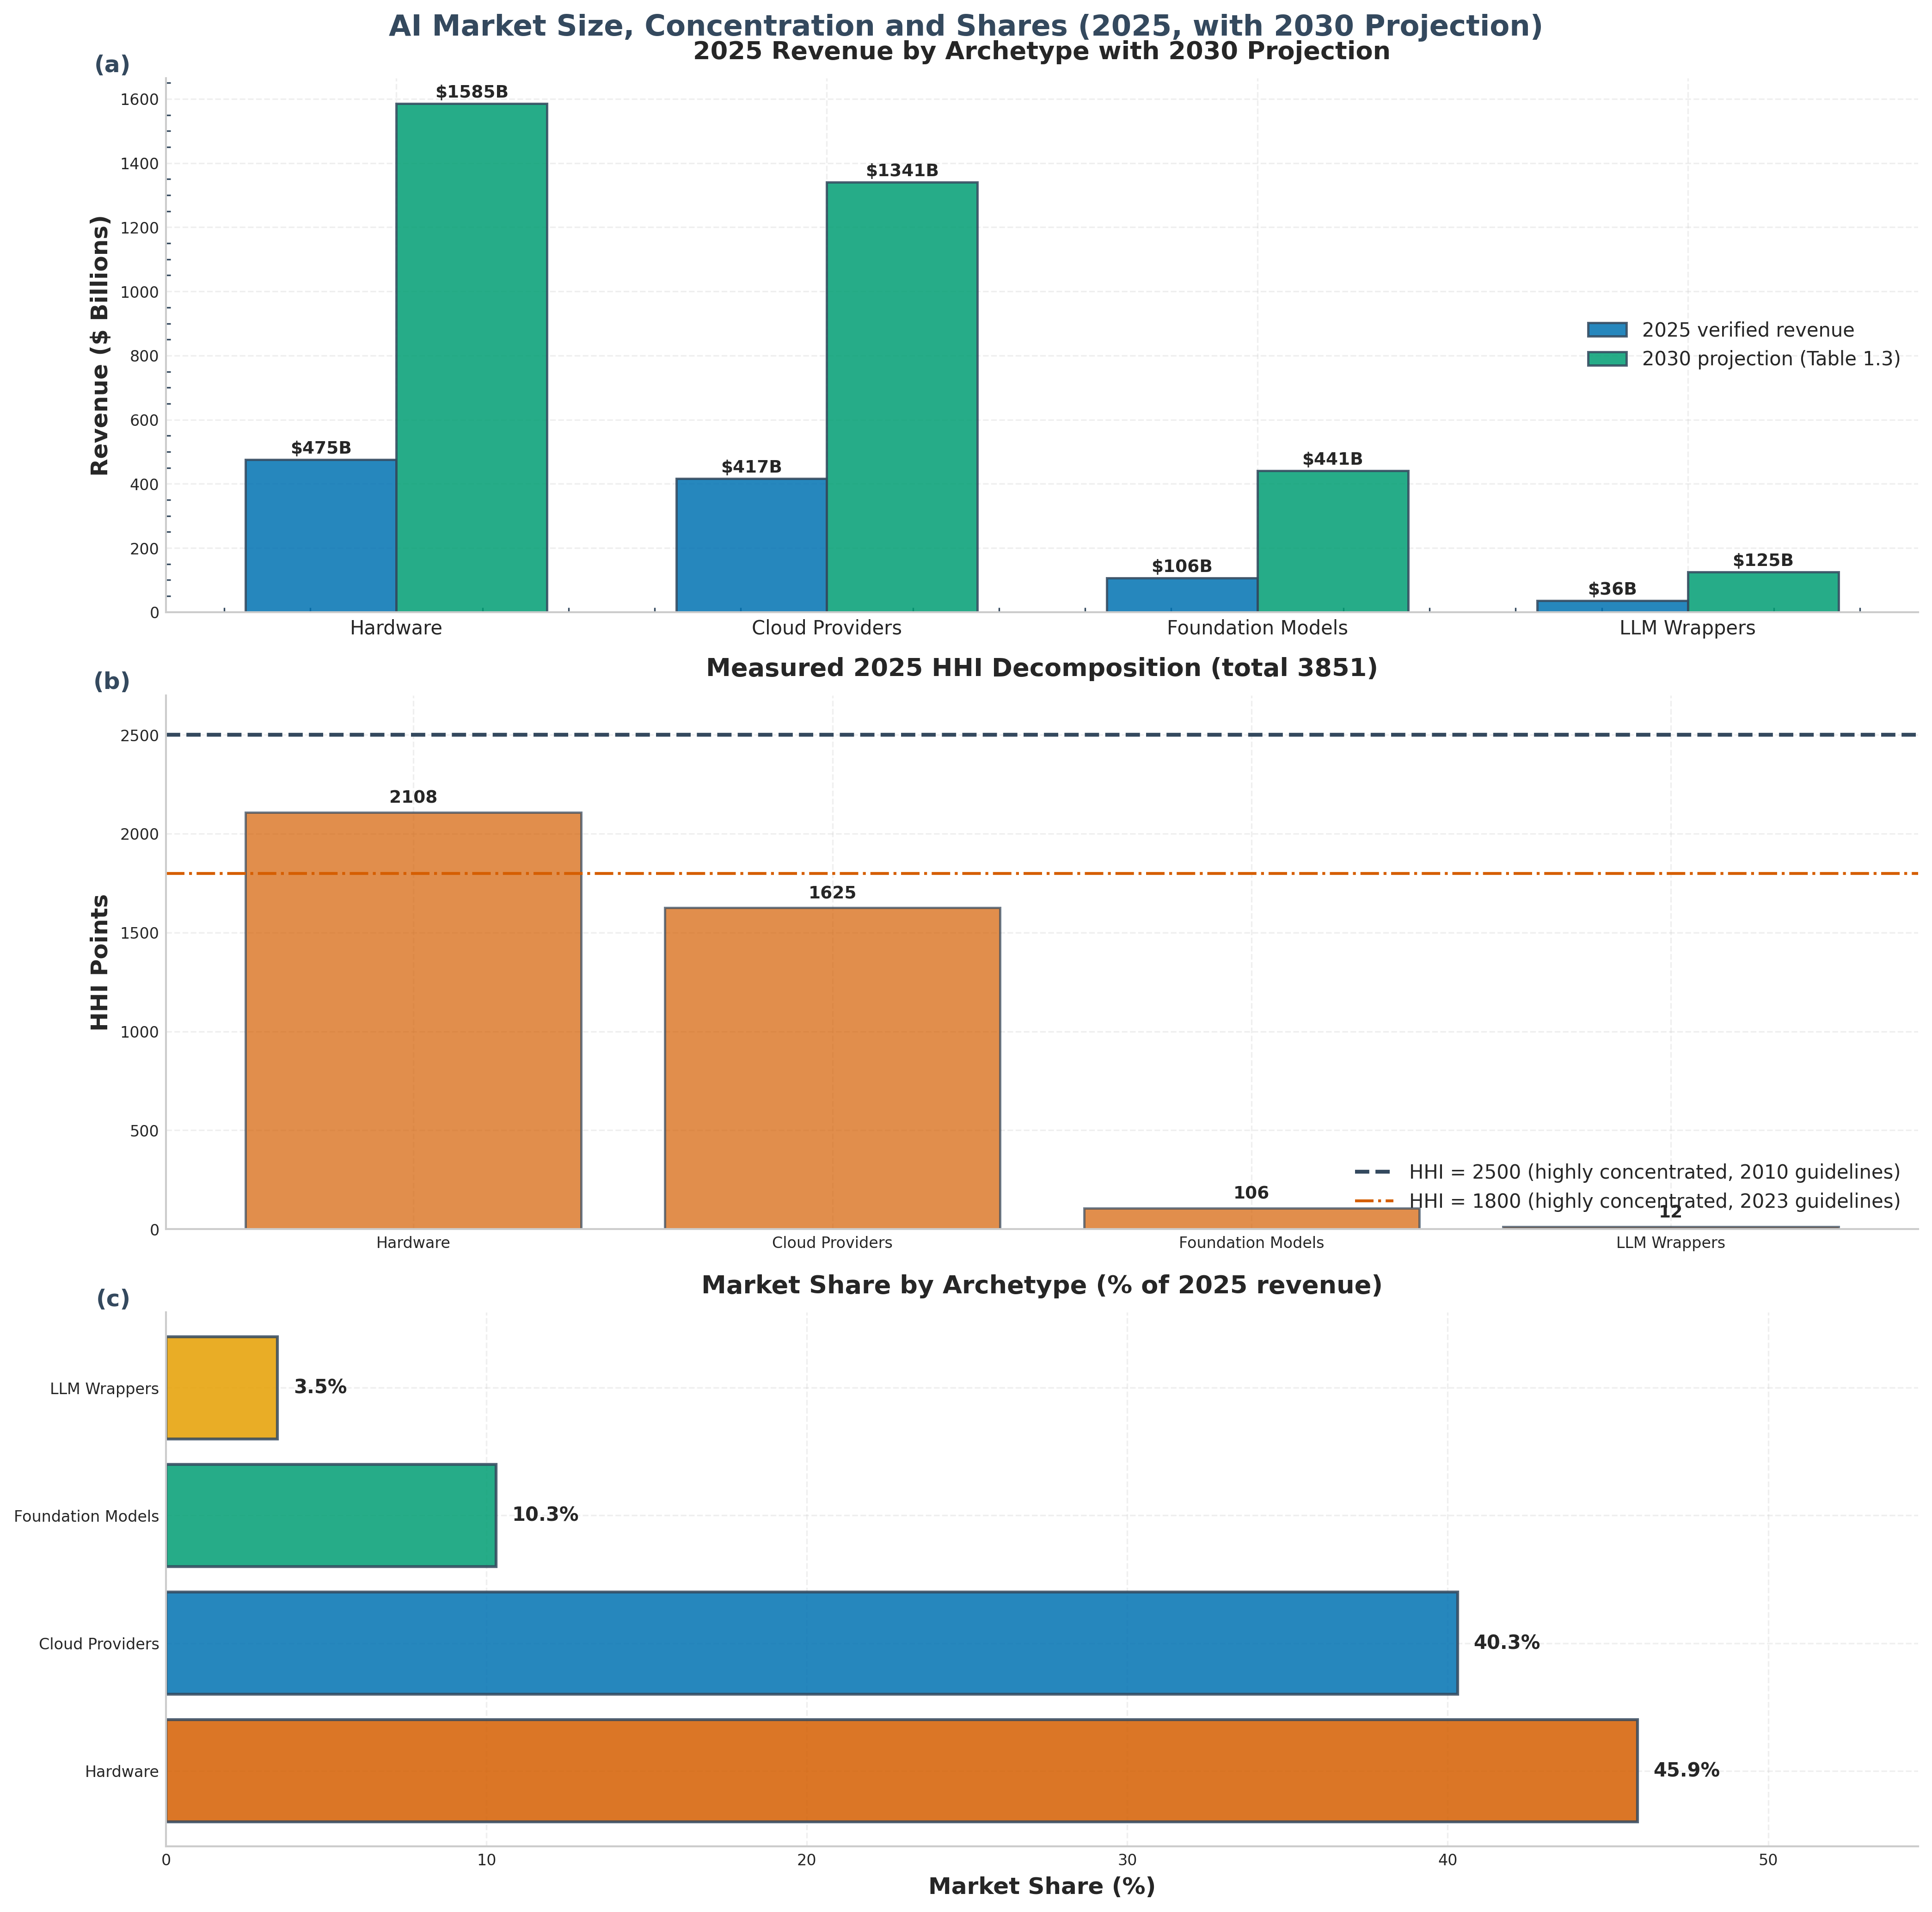
\includegraphics[width=0.72\textwidth,height=0.82\textheight,keepaspectratio]{figure_3.png}
\caption{Market size and concentration behind the prediction: 2025 revenue by archetype with the 2030 projection, the cross-stack composition index (3,851) split into archetype contributions, and revenue shares. Concentration is the reason a single relationship's failure matters at macro scale.}
    \label{fig:02-market-size-and-concentration}
\end{figure}

Prediction consequence: because one row (GPU supply, 36.9\%) and one pair
(Hardware--Cloud) dominate the frame, the burst has a chokepoint. Shocks
dissipate across diversified graphs; they detonate in concentrated ones.

\begin{figure}[htbp]
\centering
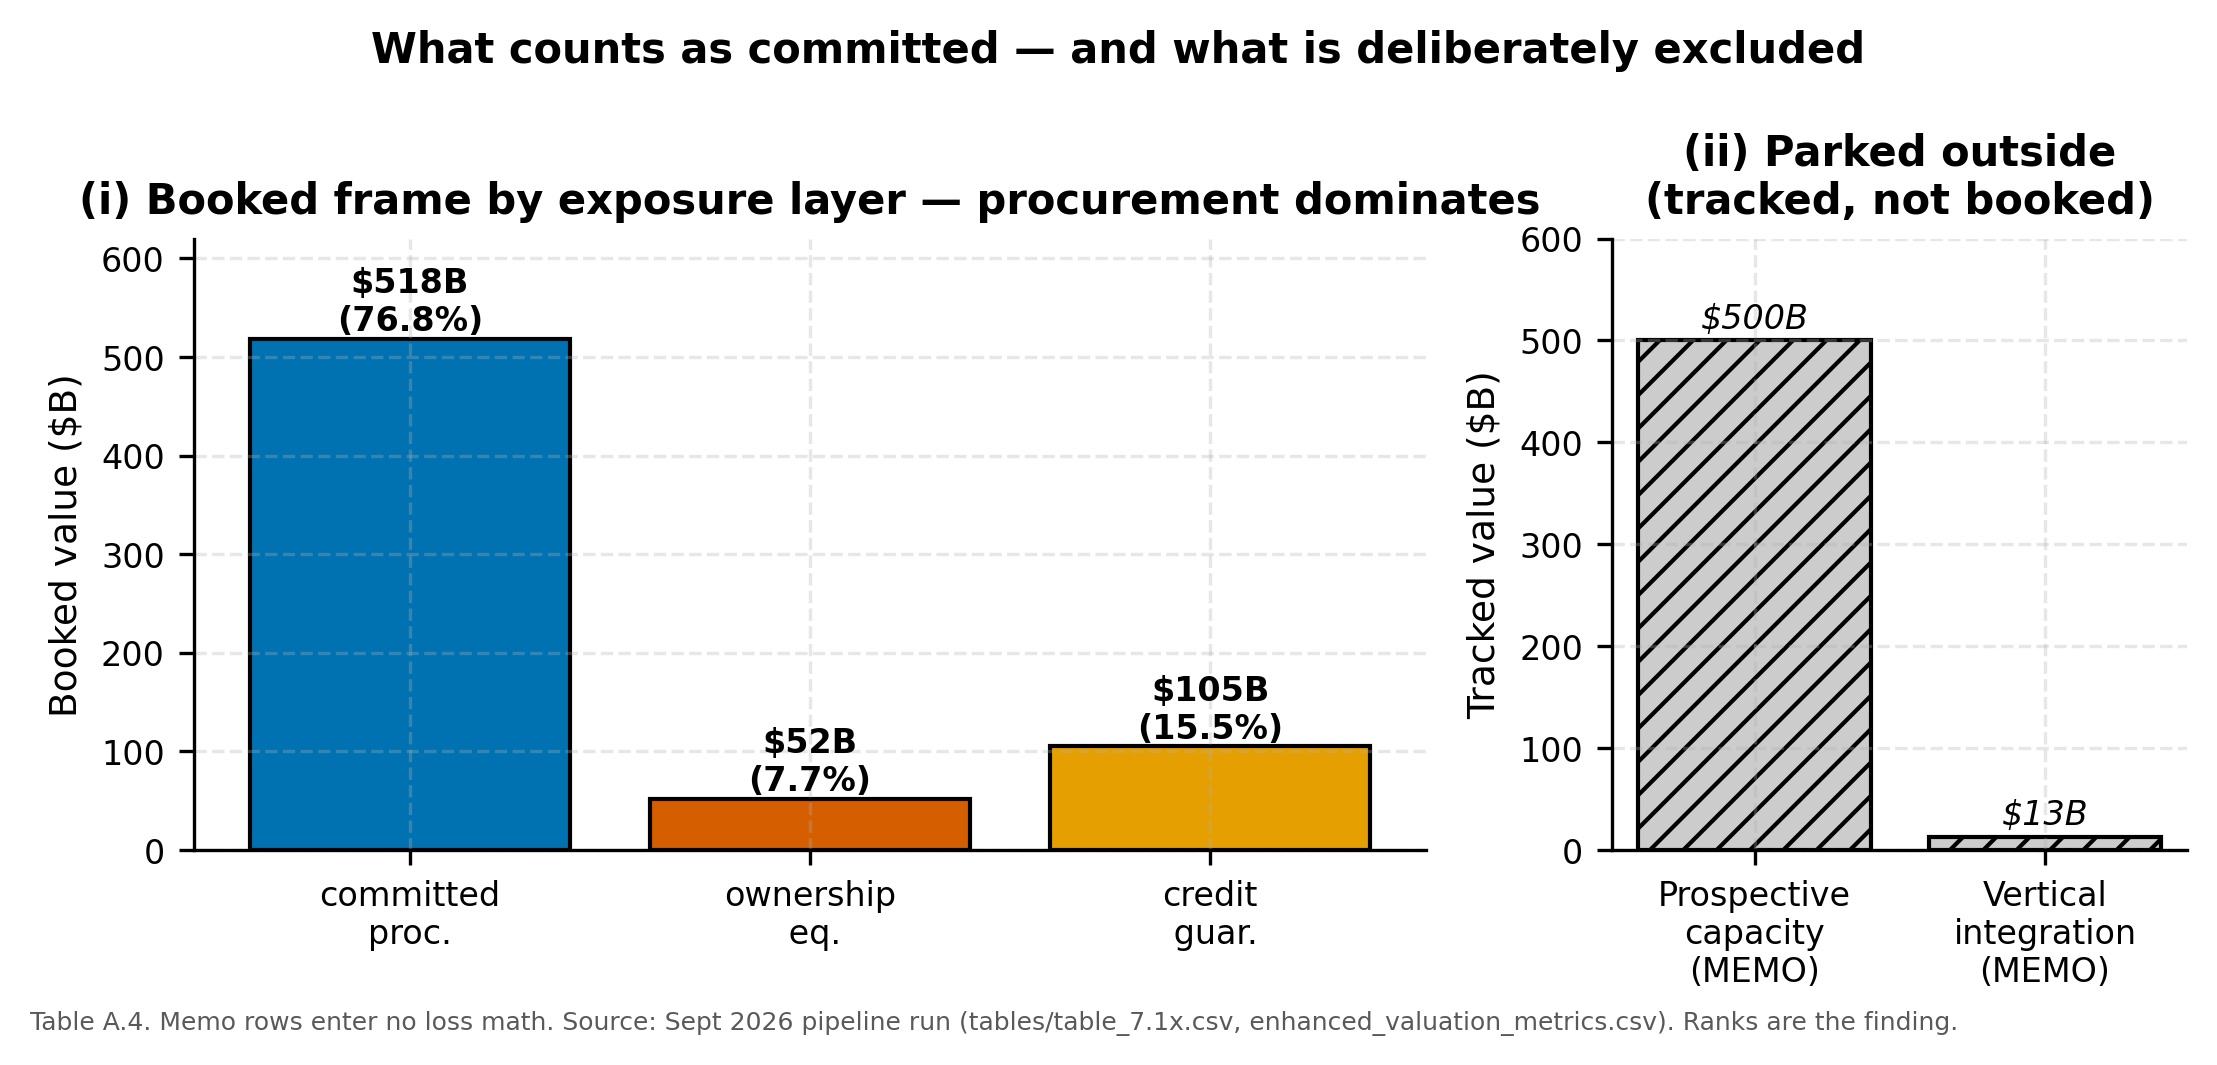
\includegraphics[width=\textwidth,height=0.82\textheight,keepaspectratio]{pred_layer_composition.png}
\caption{Booked frame by exposure layer (Table~A.4): committed procurement (\$518.4B, 76.8\%) plus the \$105B credit guarantee and \$52B of equity exposure sum to \$675.40B. The \$500B prospective facility and \$12.93B vertical-integration purchase are tracked but parked outside every loss computation --- the accounting discipline that keeps the frame auditable.}
    \label{fig:03-booked-frame-by-exposure}
\end{figure}

Layer reading: more than three-quarters of the booked frame is procurement
(payment obligations that propagate at face in DebtRank), which is why the
cascade of Section~\ref{sec:contagion} runs primarily through unpaid
compute bills rather than equity markdowns. The guarantee layer (15.5\%) is
contingent --- it pays only on default --- so it concentrates the tail:
small in the base case, outsized in the severe one.

\begin{figure}[htbp]
\centering
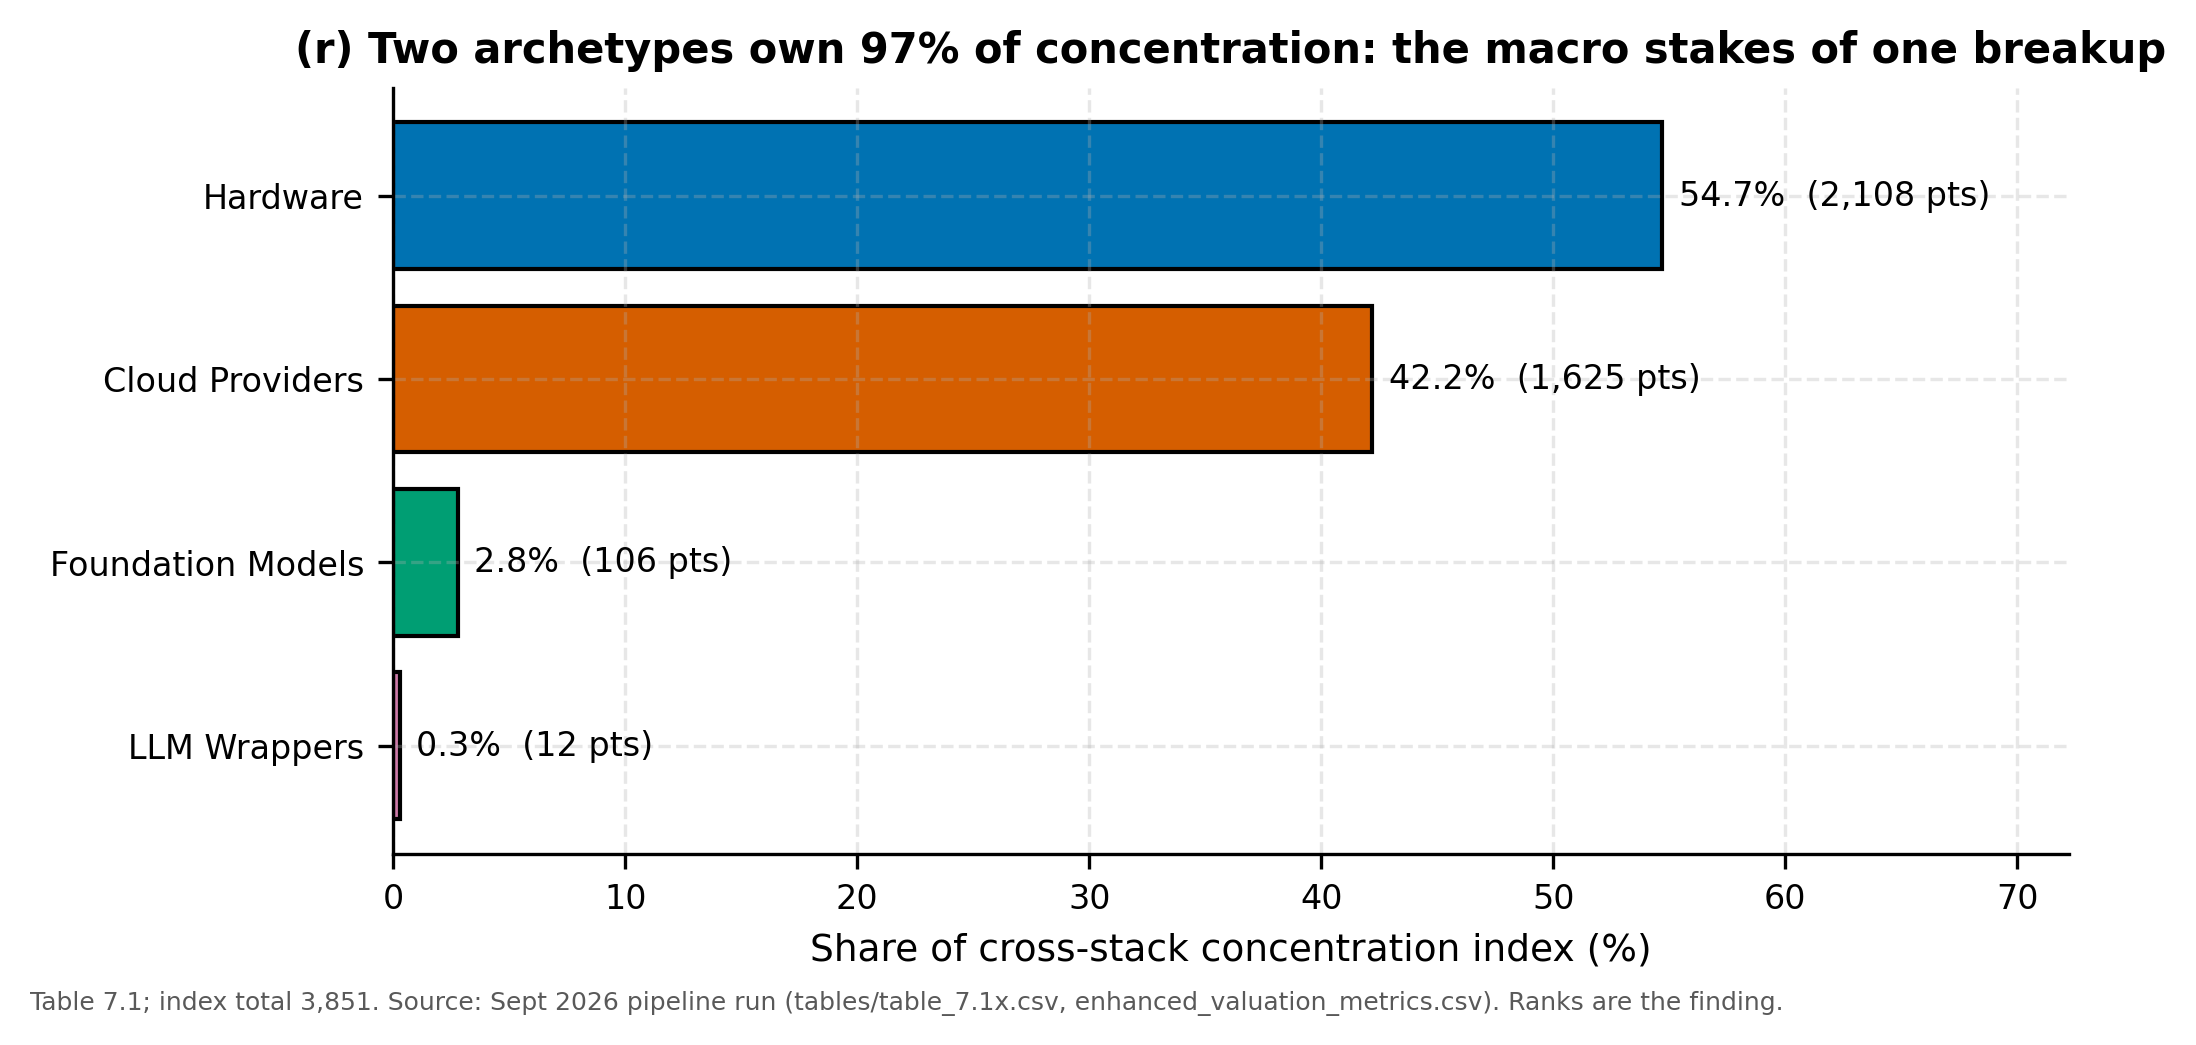
\includegraphics[width=\textwidth,height=0.82\textheight,keepaspectratio]{pred_concentration.png}
\caption{Concentration behind the prediction (Table~7.1): Hardware (54.7\%) and Cloud (42.2\%) own 97\% of the 3,851-point cross-stack index. Macro stakes live in two archetypes --- which is why one relationship's failure is a sectoral event.}
    \label{fig:32-concentration-two-archetypes-own}
\end{figure}

\section{Strategic Interaction: Six Bilateral Games and the Scope for Cooperation}\label{sec:games}
The core game is the prediction's engine, but the other five set its
boundaries. Each row below gives the stable outcome, the best-joint
outcome, the trapped value, and the payment that would unlock it.

\begin{table}[htbp]
\centering
\caption{All six games: stable vs.\ best-joint welfare (\$B).}
    \label{tab:02-all-six-games-stable}
\begin{tabular}{lcccc}
\toprule
Game & Nash & Joint max & Trapped & Transfer to unlock \\
\midrule
HW--Cloud & 1,094.8 & 1,153.4 & 58.6 & 176.0 (HW to Cloud) \\
HW--Foundation & 671.3 & 876.9 & 205.6 & 46.7 (HW to FM) \\
HW--Wrappers & 609.0 & 856.1 & 247.0 & 18.7 (HW to Wrappers) \\
Cloud--Foundation & 604.1 & 745.4 & 141.2 & 46.3 (Cloud to FM) \\
Cloud--Wrappers & 544.3 & 725.0 & 180.7 & 18.7 (Cloud to Wrappers) \\
FM--Wrappers & 142.5 & 177.1 & 34.6 & 1.1 (FM to Wrappers) \\
\midrule
\textbf{Diagnostic sum} & & & \textbf{867.8} & \textbf{307.4} \\
\bottomrule
\end{tabular}
\end{table}

Three prediction readings. \emph{First}, the largest trapped value
(\$247.0B, Hardware--Wrappers) needs the smallest key (\$18.7B): the
cheapest cooperation in the stack is also among the most valuable, which is
where a negotiated settlement would start. \emph{Second}, every unlock
payment flows upstream-to-downstream, so in a crisis the kill chain runs
through whoever refuses to pay --- watch Hardware's and Cloud's willingness
to compensate, not the labs'. \emph{Third}, the core game's \$176.0B price
tag on a \$58.6B gain is the worst ratio in the stack: the most important
cooperation is the least likely to happen voluntarily, which is why it needs
regulation rather than hope. (The \$867.8B sum multi-counts shared players
across pairs; the \$416.77B top-down bound, not this sum, sizes policy.)

Standard Coasean bargaining cannot be expected to unlock the core cell.
The Cloud provider's GPU-obsolescence exposure --- generation lifecycles of
18--24 months against 5-year accounting depreciation --- is unobservable to
the Hardware side, so no compensating payment clears at fair value. The
deeper block is hold-up under vertical asset specificity
\citep{klein1978,williamson1985}: because GPU clusters exhibit extreme
physical and temporal specificity, neither counterparty can commit ex ante
to long-term surplus sharing without vertical integration or formal credit
wraps --- which is why the unselected Pareto cell cannot be reached via
private contracting alone.

\begin{figure}[htbp]
\centering
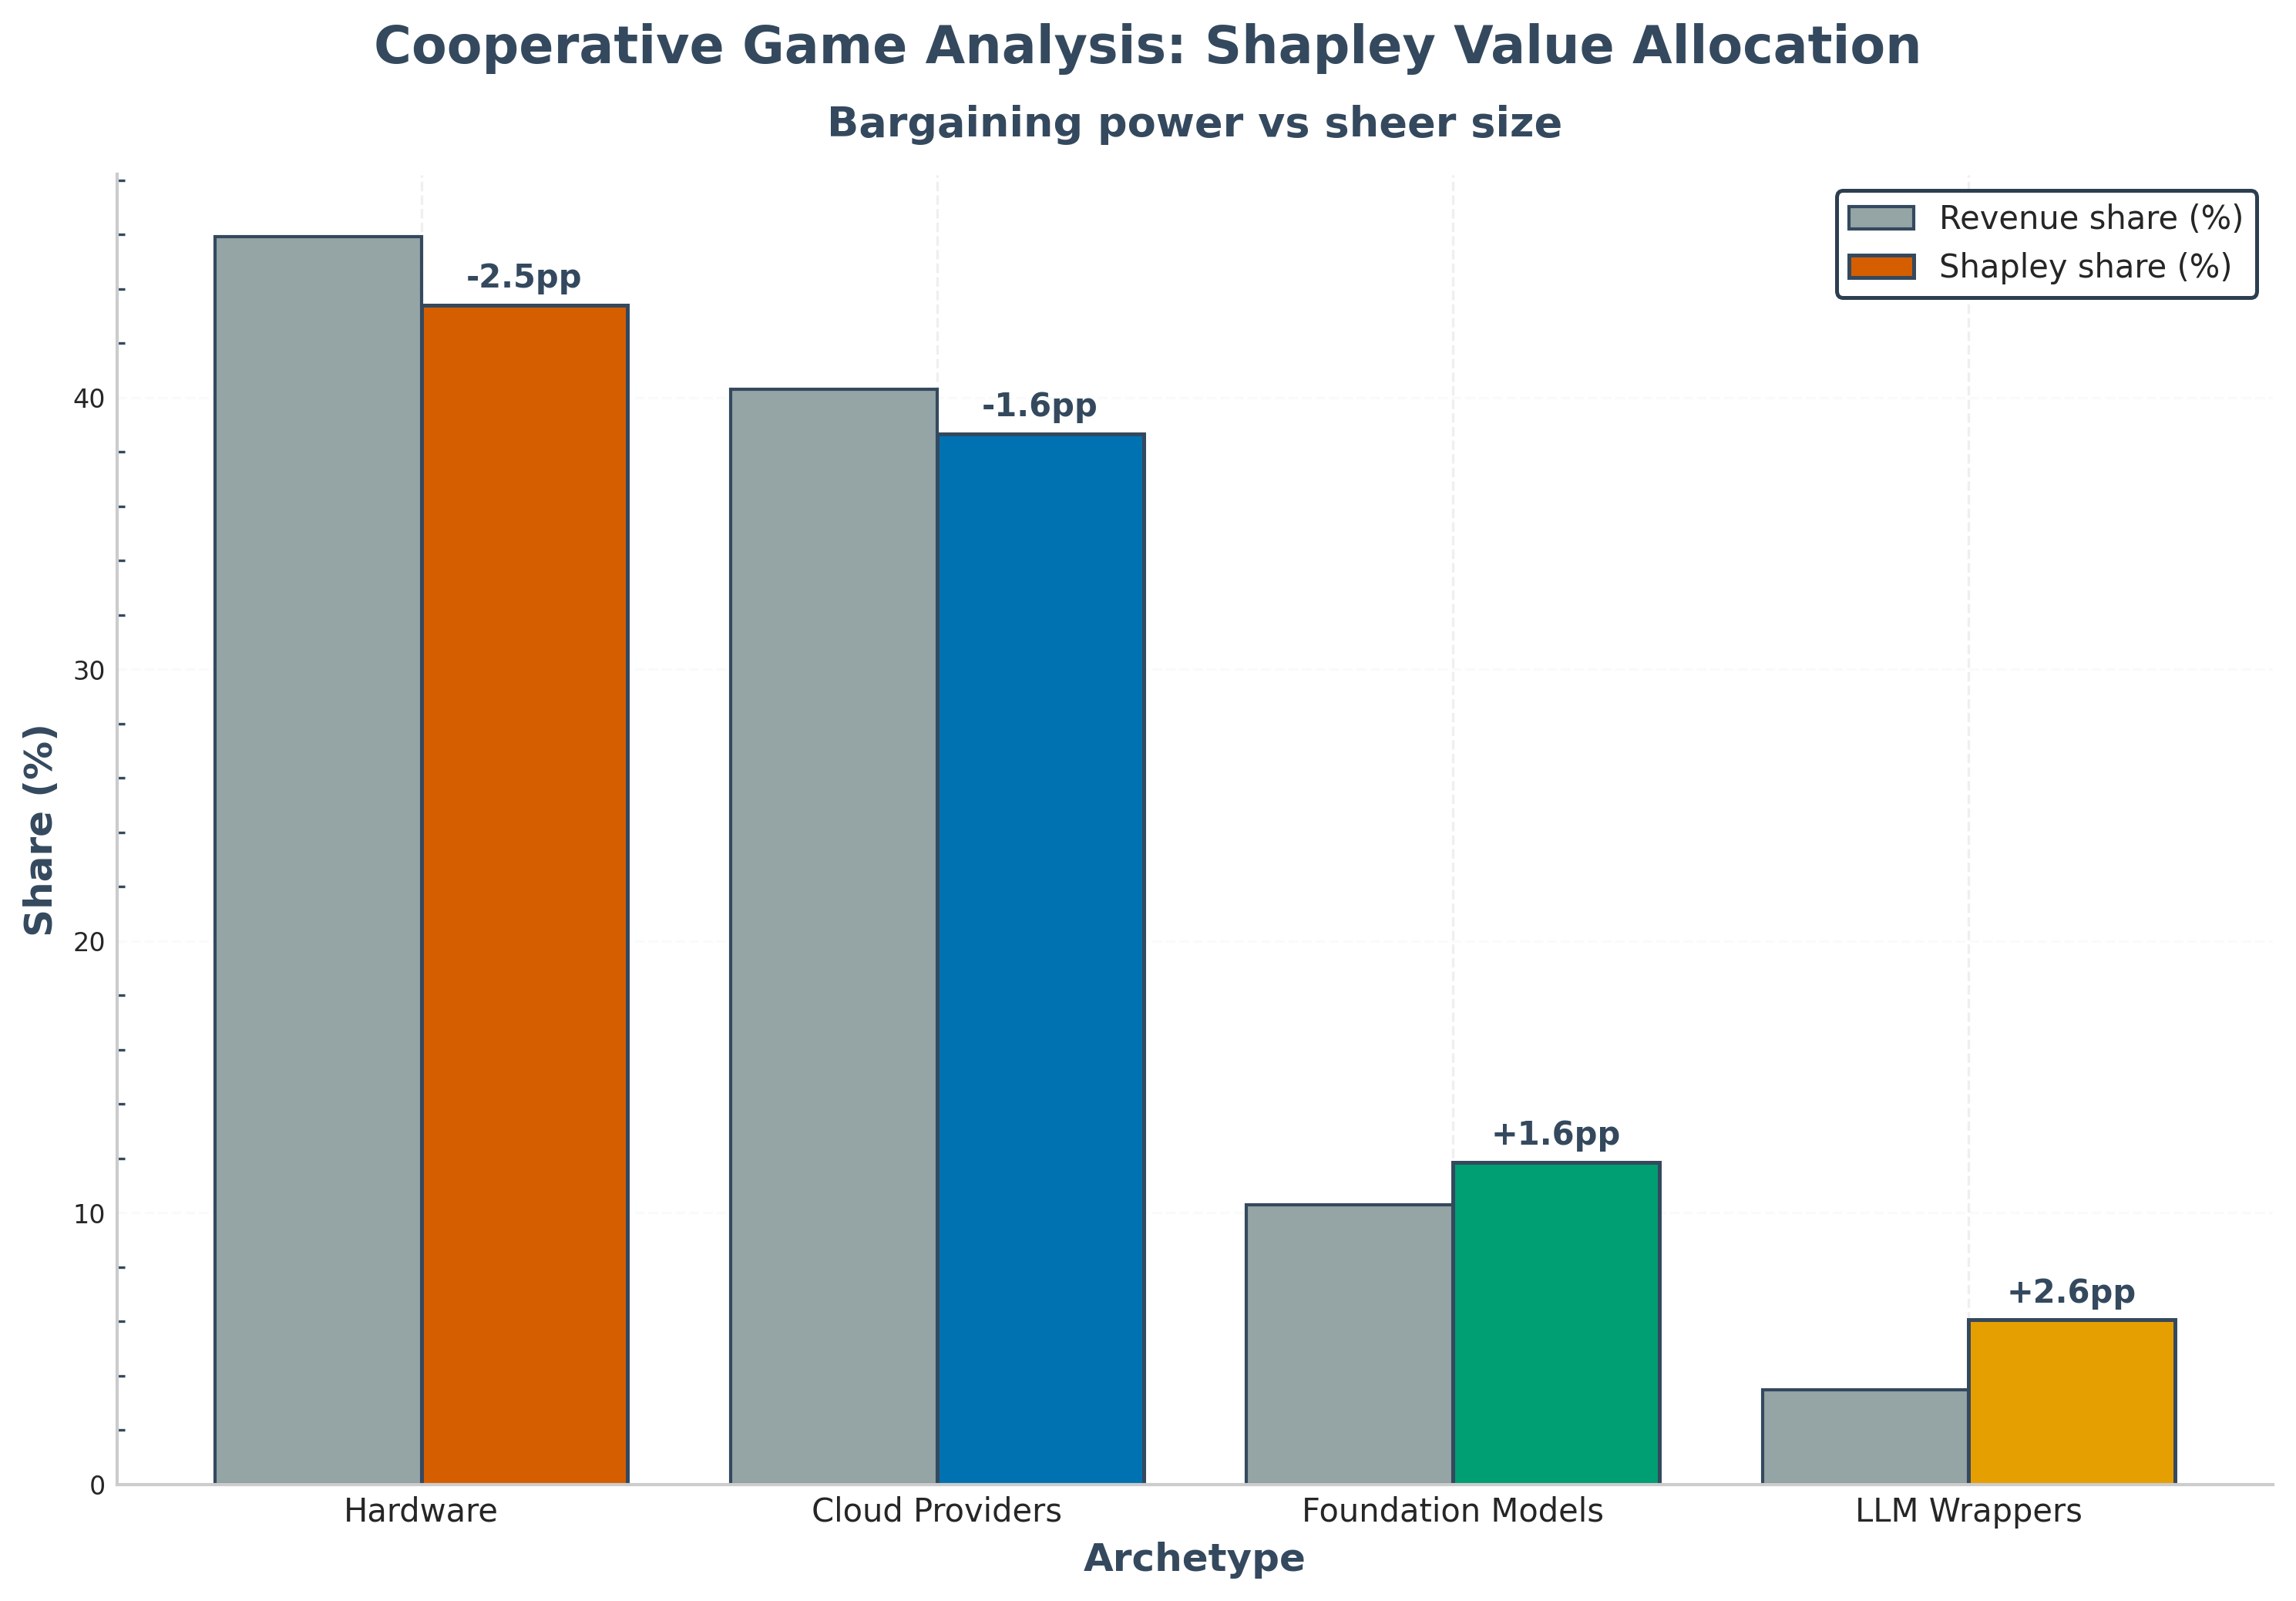
\includegraphics[width=0.85\textwidth,height=0.82\textheight,keepaspectratio]{figure_16.png}
\caption{Cooperative benchmark: Shapley values vs.\ revenue shares (Table~7.18). Hardware (43.4\% Shapley on 45.9\% revenue) and Cloud (38.7\% on 40.3\%) capture slightly less than they earn, while Wrappers capture more than they earn (6.1\% vs.\ 3.5\%) --- downstream players free-ride on upstream investment, which is exactly why upstream-to-downstream transfers are needed to unlock cooperation.}
    \label{fig:04-cooperative-benchmark-shapley-values}
\end{figure}

\begin{figure}[htbp]
\centering
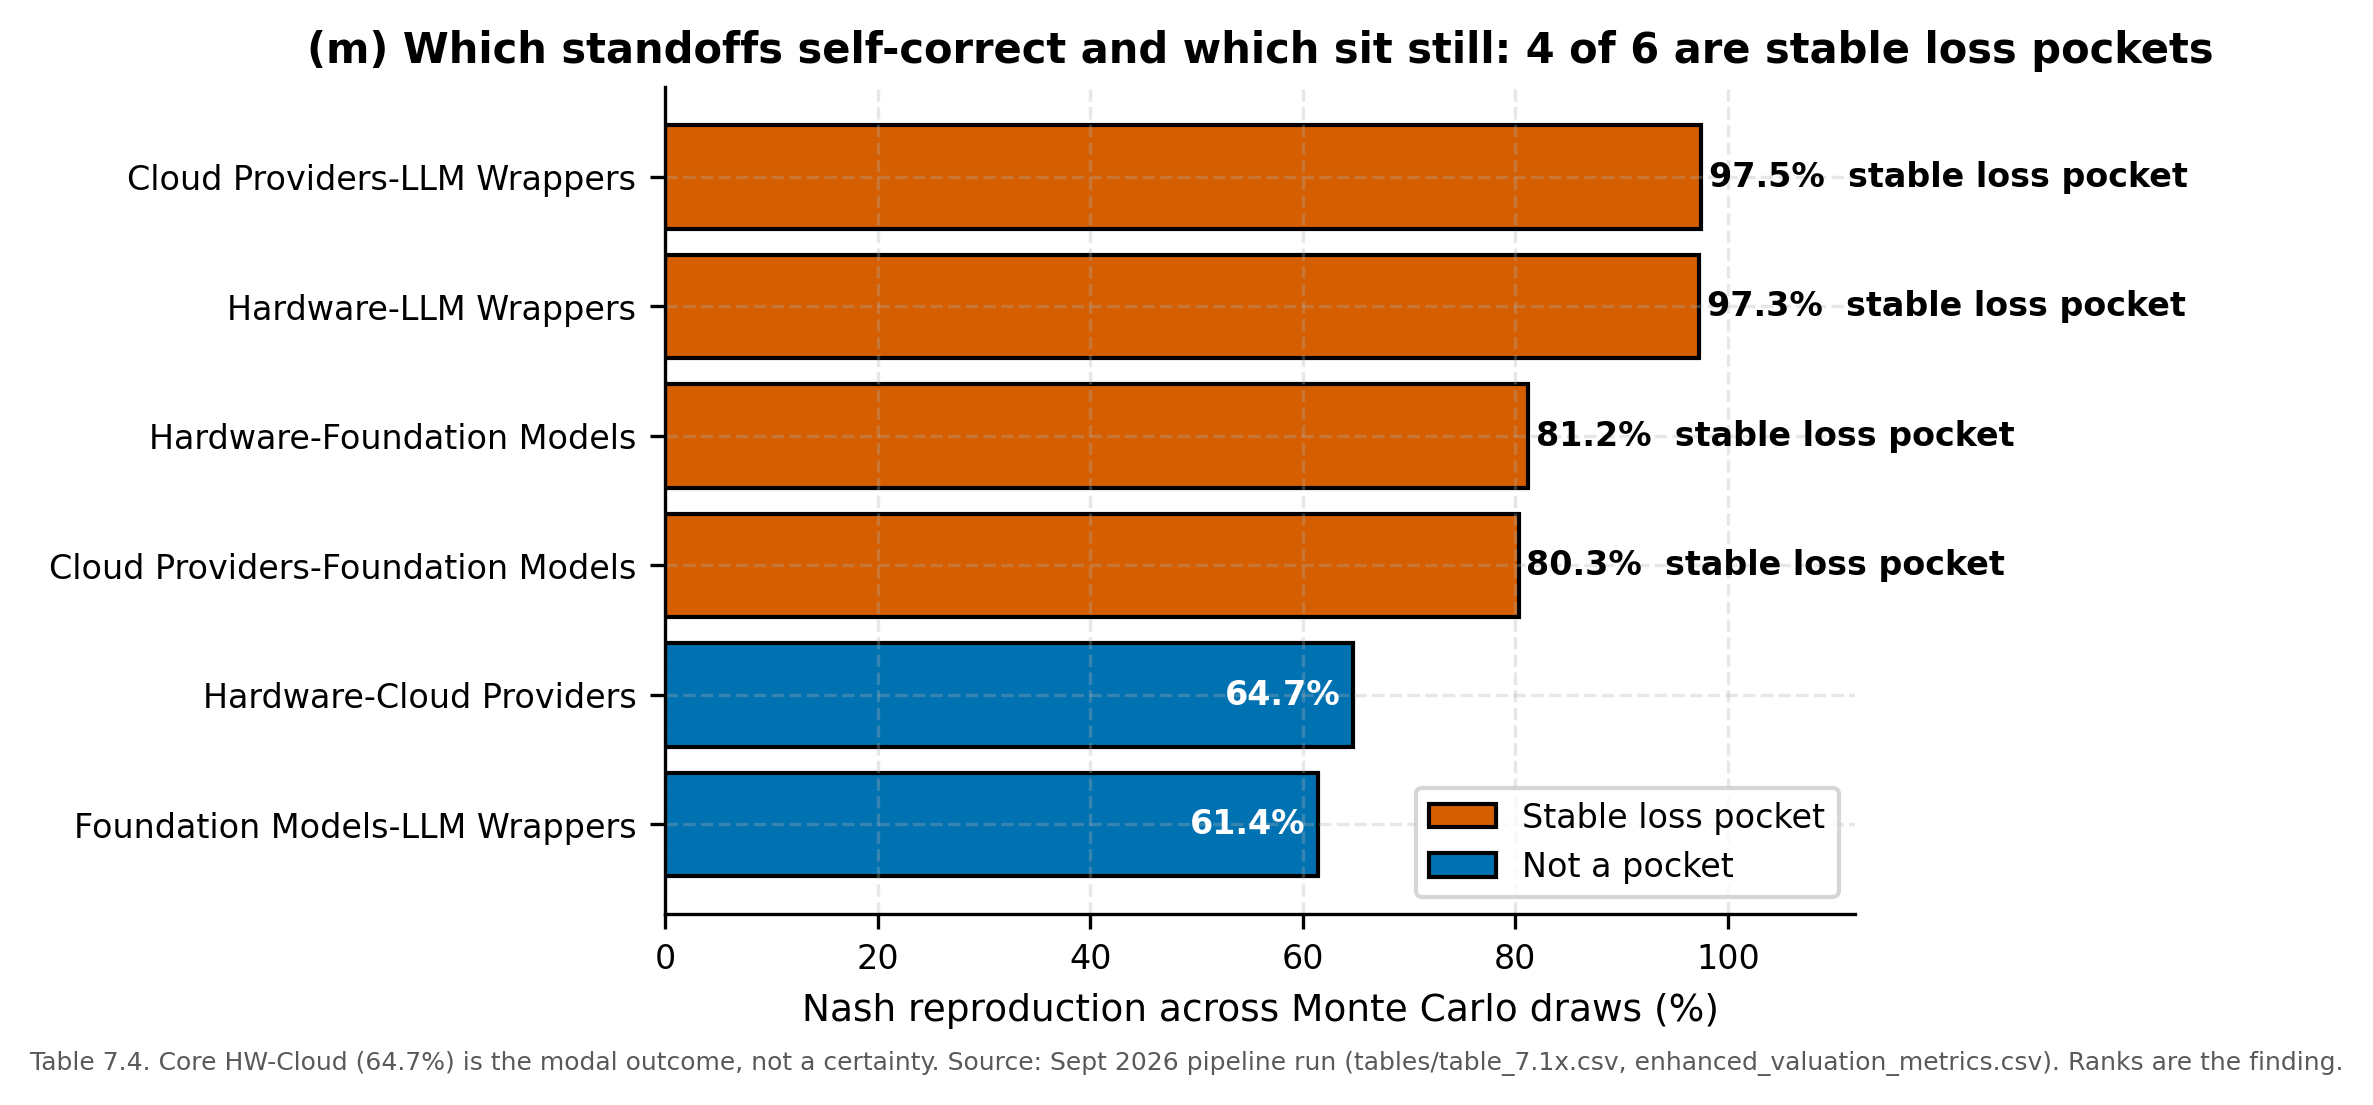
\includegraphics[width=\textwidth,height=0.82\textheight,keepaspectratio]{pred_stability_pockets.png}
\caption{Equilibrium stability screen (Table~7.4): how often each game's Nash outcome reproduces across Monte Carlo draws. Four of six games are stable loss pockets ($\geq$80\%) --- they will sit in their stuck cells indefinitely. The core Hardware--Cloud game is the exception at 64.7\%: its stuck cell is the modal outcome, not a certainty, so watch it for the first sign of either negotiated settlement or disorderly break.}
    \label{fig:05-equilibrium-stability-screen-table74}
\end{figure}

Stability sharpens the prediction's timing logic. The four peripheral games
will not self-correct --- their Nash cells reproduce nearly every draw, so
waiting for voluntary cooperation there is waiting for nothing. The core
game, less stable, is where movement happens first in either direction:
settlement (watch for the \$176B transfer being negotiated down) or rupture
(watch the trigger framework of Section~\ref{sec:triggers}). Note what this
does \emph{not} threaten: P2's $\sim$90\% burst ranking, which follows
contracts rather than equilibria --- even in draws where the core game
flips, the loss address does not move.

\section{The Binding Constraint: Non-Cooperation in the Hardware--Cloud Game}\label{sec:core}
Six pairwise standoffs were solved. All six trap value absent cooperation,
but only one binds the prediction: Hardware vs.\ Cloud. Chipmakers stay
open while clouds stay locked
in --- neither side wants to move alone --- trapping \$58.6B that
cooperation would unlock (94.9\% efficient). That single stuck relationship,
sitting on the largest contract base in the stack, is the structural reason
a repricing becomes a loss rather than a shrug.

\begin{table}[htbp]
\centering
\caption{The core Hardware--Cloud game (\$B). The stuck cell is the selected equilibrium; the best-joint cell is Nash too --- payoff- and risk-dominant --- but unselected, so persistence of the inferior cell is a lock-in story, not an incentives story.}
    \label{tab:03-the-core-hardwarecloud-game}
\begin{tabular}{lcc}
\toprule
 & Cloud: Open & Cloud: Locked (Nash) \\
\midrule
Hardware: Open (Nash) & --- & 487.9 + 606.8 = 1,094.8 \\
Hardware: Walled (Pareto) & 722.5 + 430.8 = 1,153.4 & --- \\
\bottomrule
\end{tabular}
\end{table}

\begin{figure}[htbp]
\centering
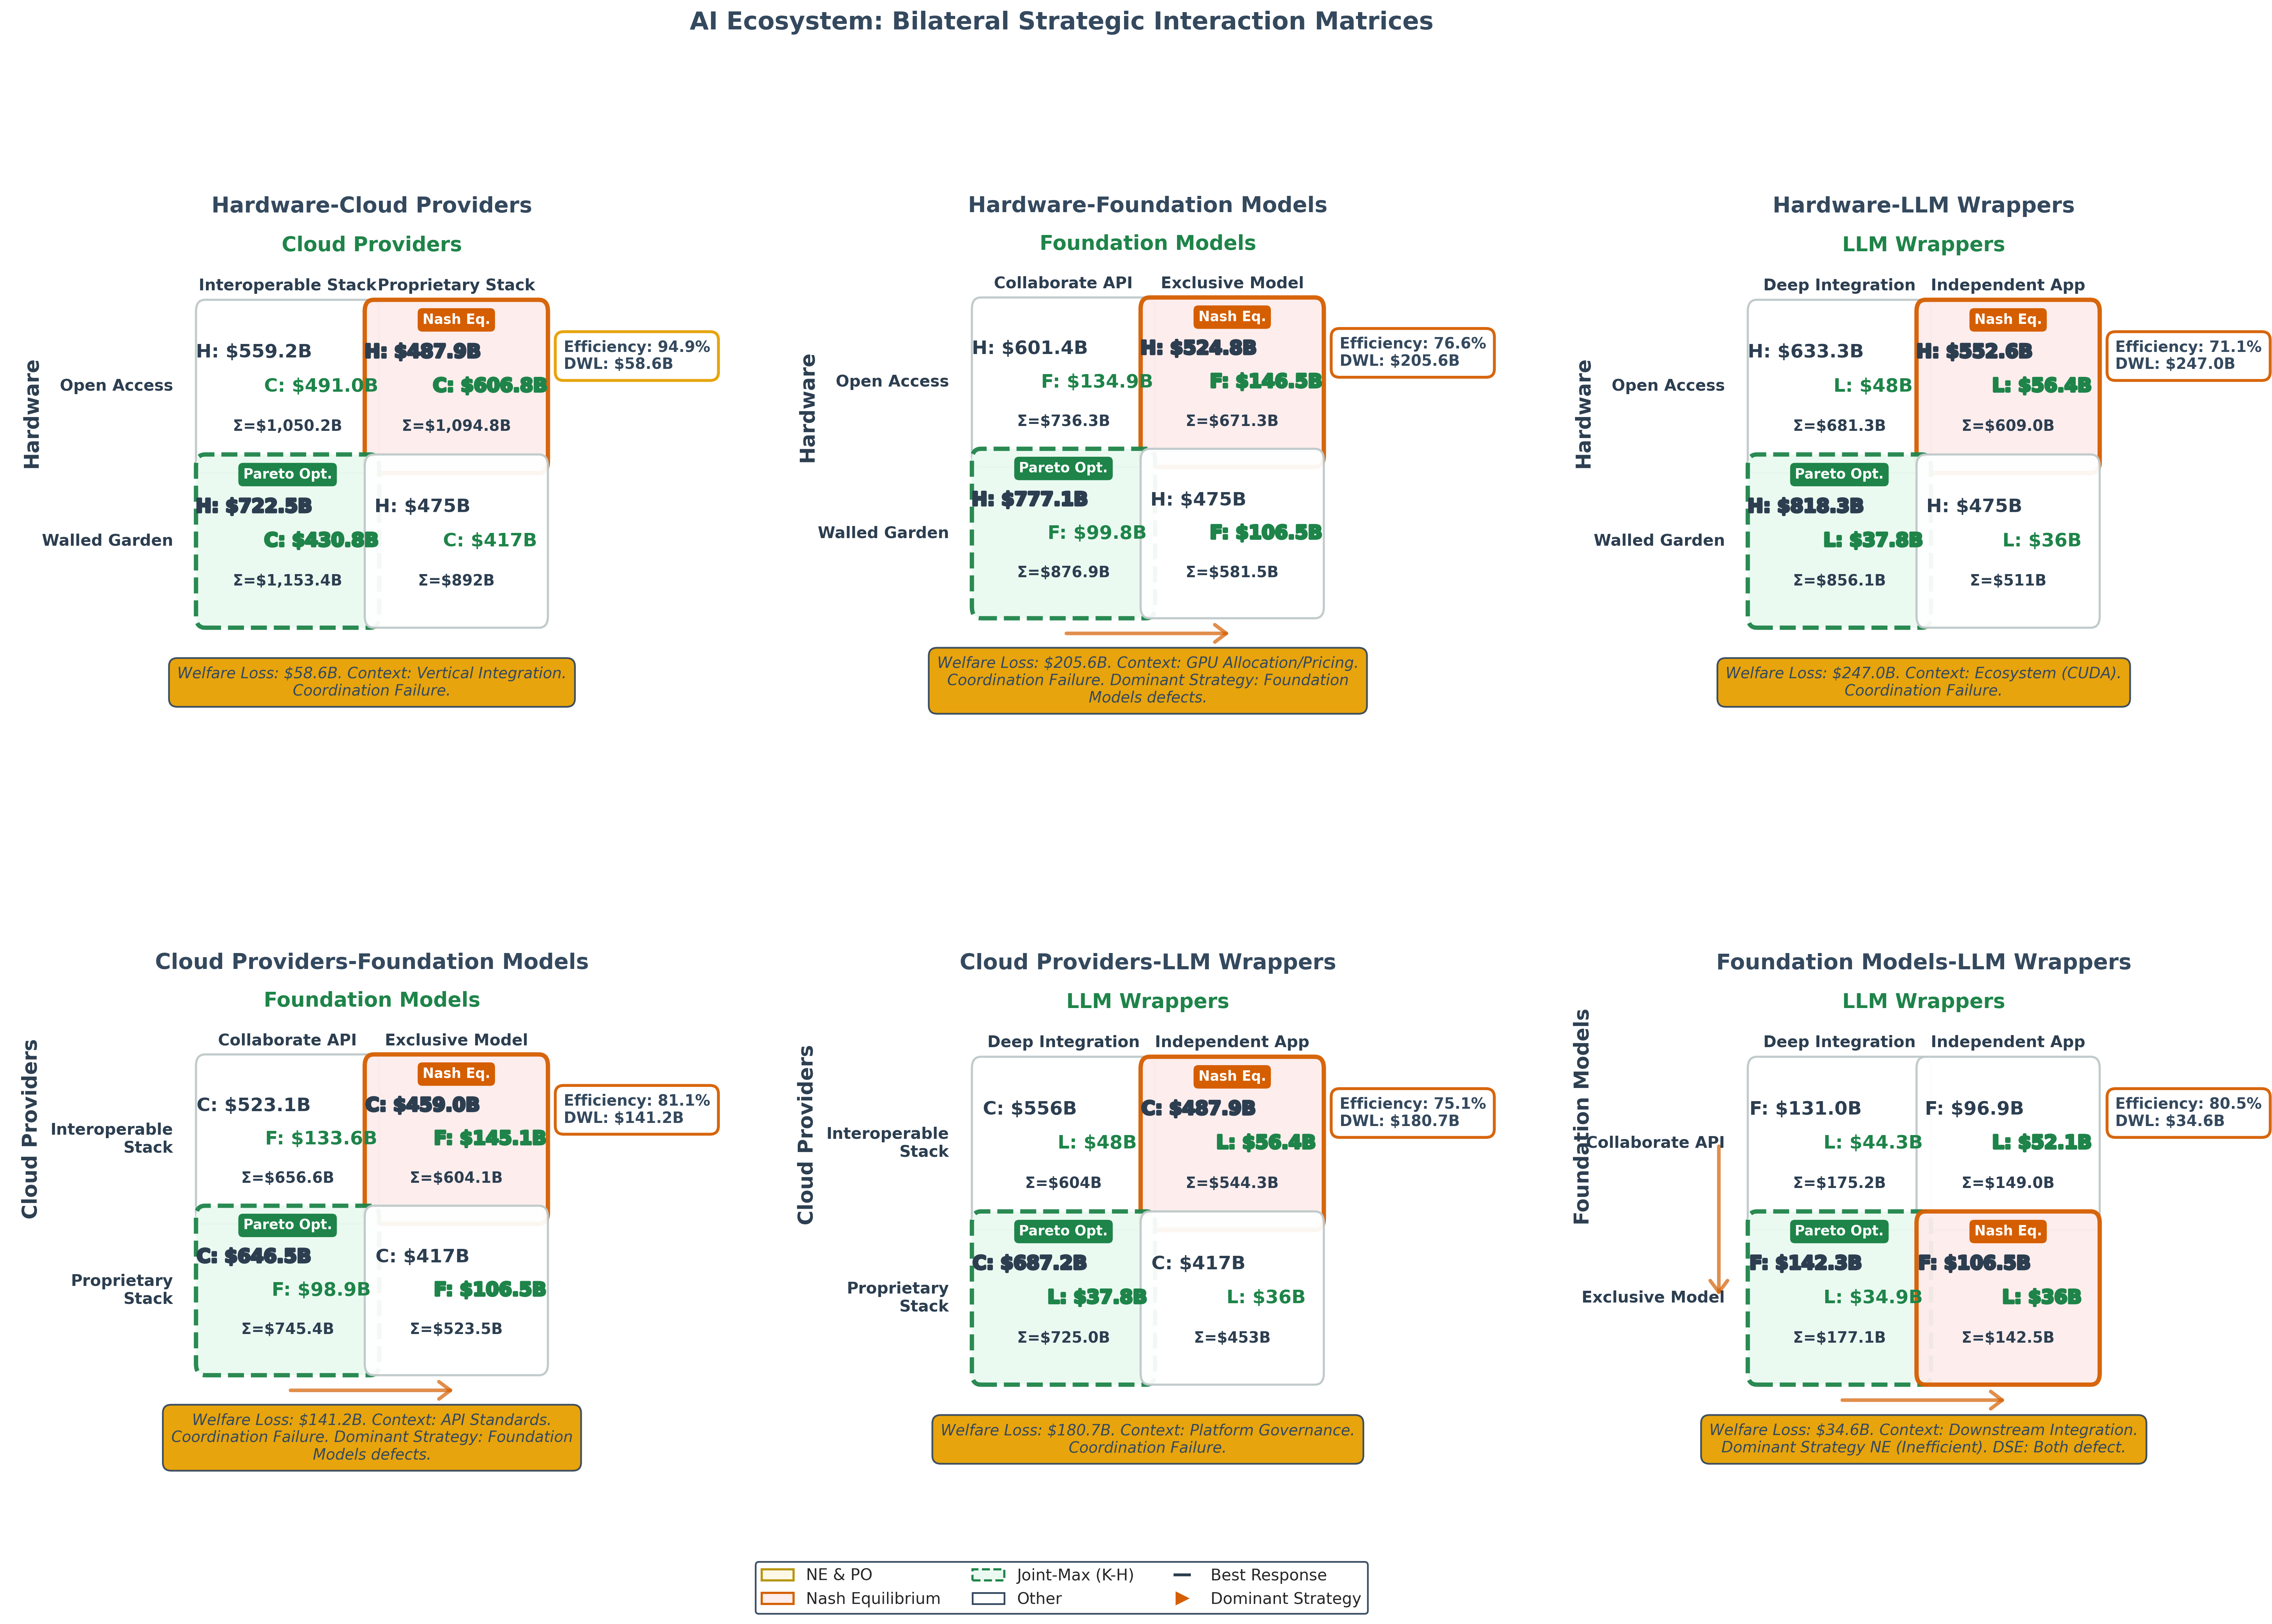
\includegraphics[width=0.85\textwidth,height=0.82\textheight,keepaspectratio]{figure_5.png}
\caption{All six pairwise standoffs with stable and best-joint cells marked. Only the infrastructure core binds --- the prediction's single bottleneck.}
    \label{fig:06-all-six-pairwise-standoffs}
\end{figure}

\begin{figure}[htbp]
\centering
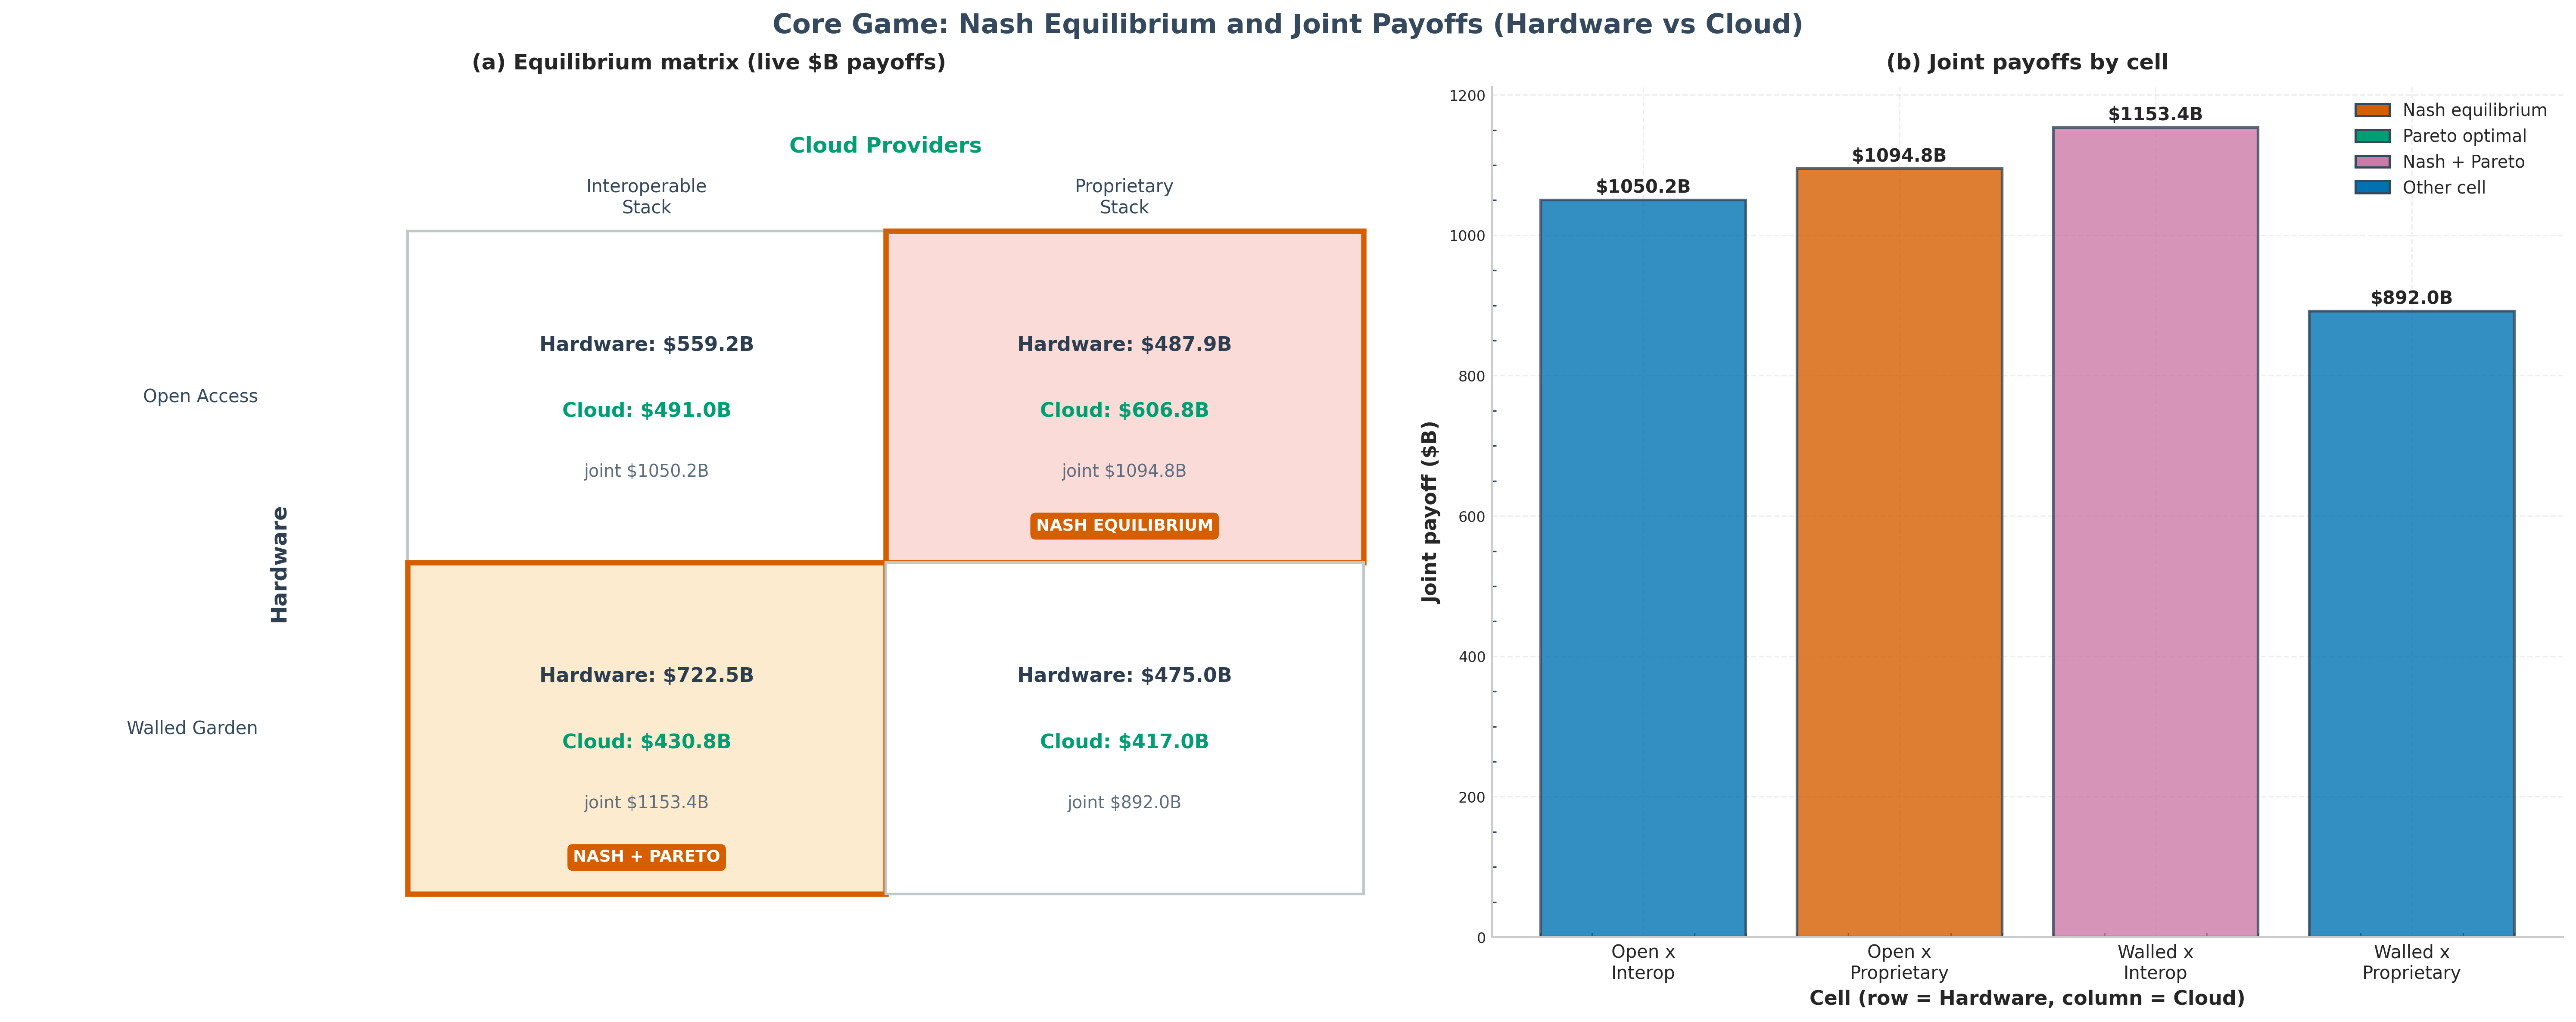
\includegraphics[width=\textwidth,height=0.82\textheight,keepaspectratio]{figure_6.png}
\caption{The core game up close: the lock-in cell maximizes neither player's payoff alone but is unilaterally stable. Unlocking it requires a \$176.0B compensating transfer from Hardware to Cloud --- the price of the \$58.6B joint gain.}
    \label{fig:07-the-core-game-up}
\end{figure}

Two audits sharpen the reading. The multiplicity audit (Table~3.6) finds the
core game's efficient outcome is both payoff- and risk-dominant --- yet the
stack sits in the inferior cell anyway, which means lock-in and history, not
incentives, hold it there, and only an outside force (regulation or crisis)
moves it. The repeated-game audit (Table~3.7) finds cooperation sustainable
without transfers in three of six games --- including the core --- while the
three Foundation-Model games cannot sustain cooperation at any patience
level (Nash reversion is not a credible punishment there). So the periphery
needs commitment devices, the core needs a push, and the labs need
supervision: three different remedies for three different audit verdicts.

\section{Welfare Analysis: Decomposition of Deadweight Loss}\label{sec:welfare}
The stuck games waste \$416.77B in total, itemized in Table~\ref{tab:04-waste-by-source-b}.
The prediction-relevant fact is the ordering, which survives every stress test:
lock-in first (\$142.62B), distorted R\&D second (\$106.97B). Remedies aimed
anywhere else are aimed at smaller problems. Each category has a canonical
antecedent: switching costs \citep{klemperer1987,farrell2007}, innovation
distortion \citep{aghion2005}, quality degradation \citep{spence1975},
coordination failures \citep{cooper1988}, and monopoly markups
\citep{harberger1954}.

\begin{figure}[htbp]
\centering
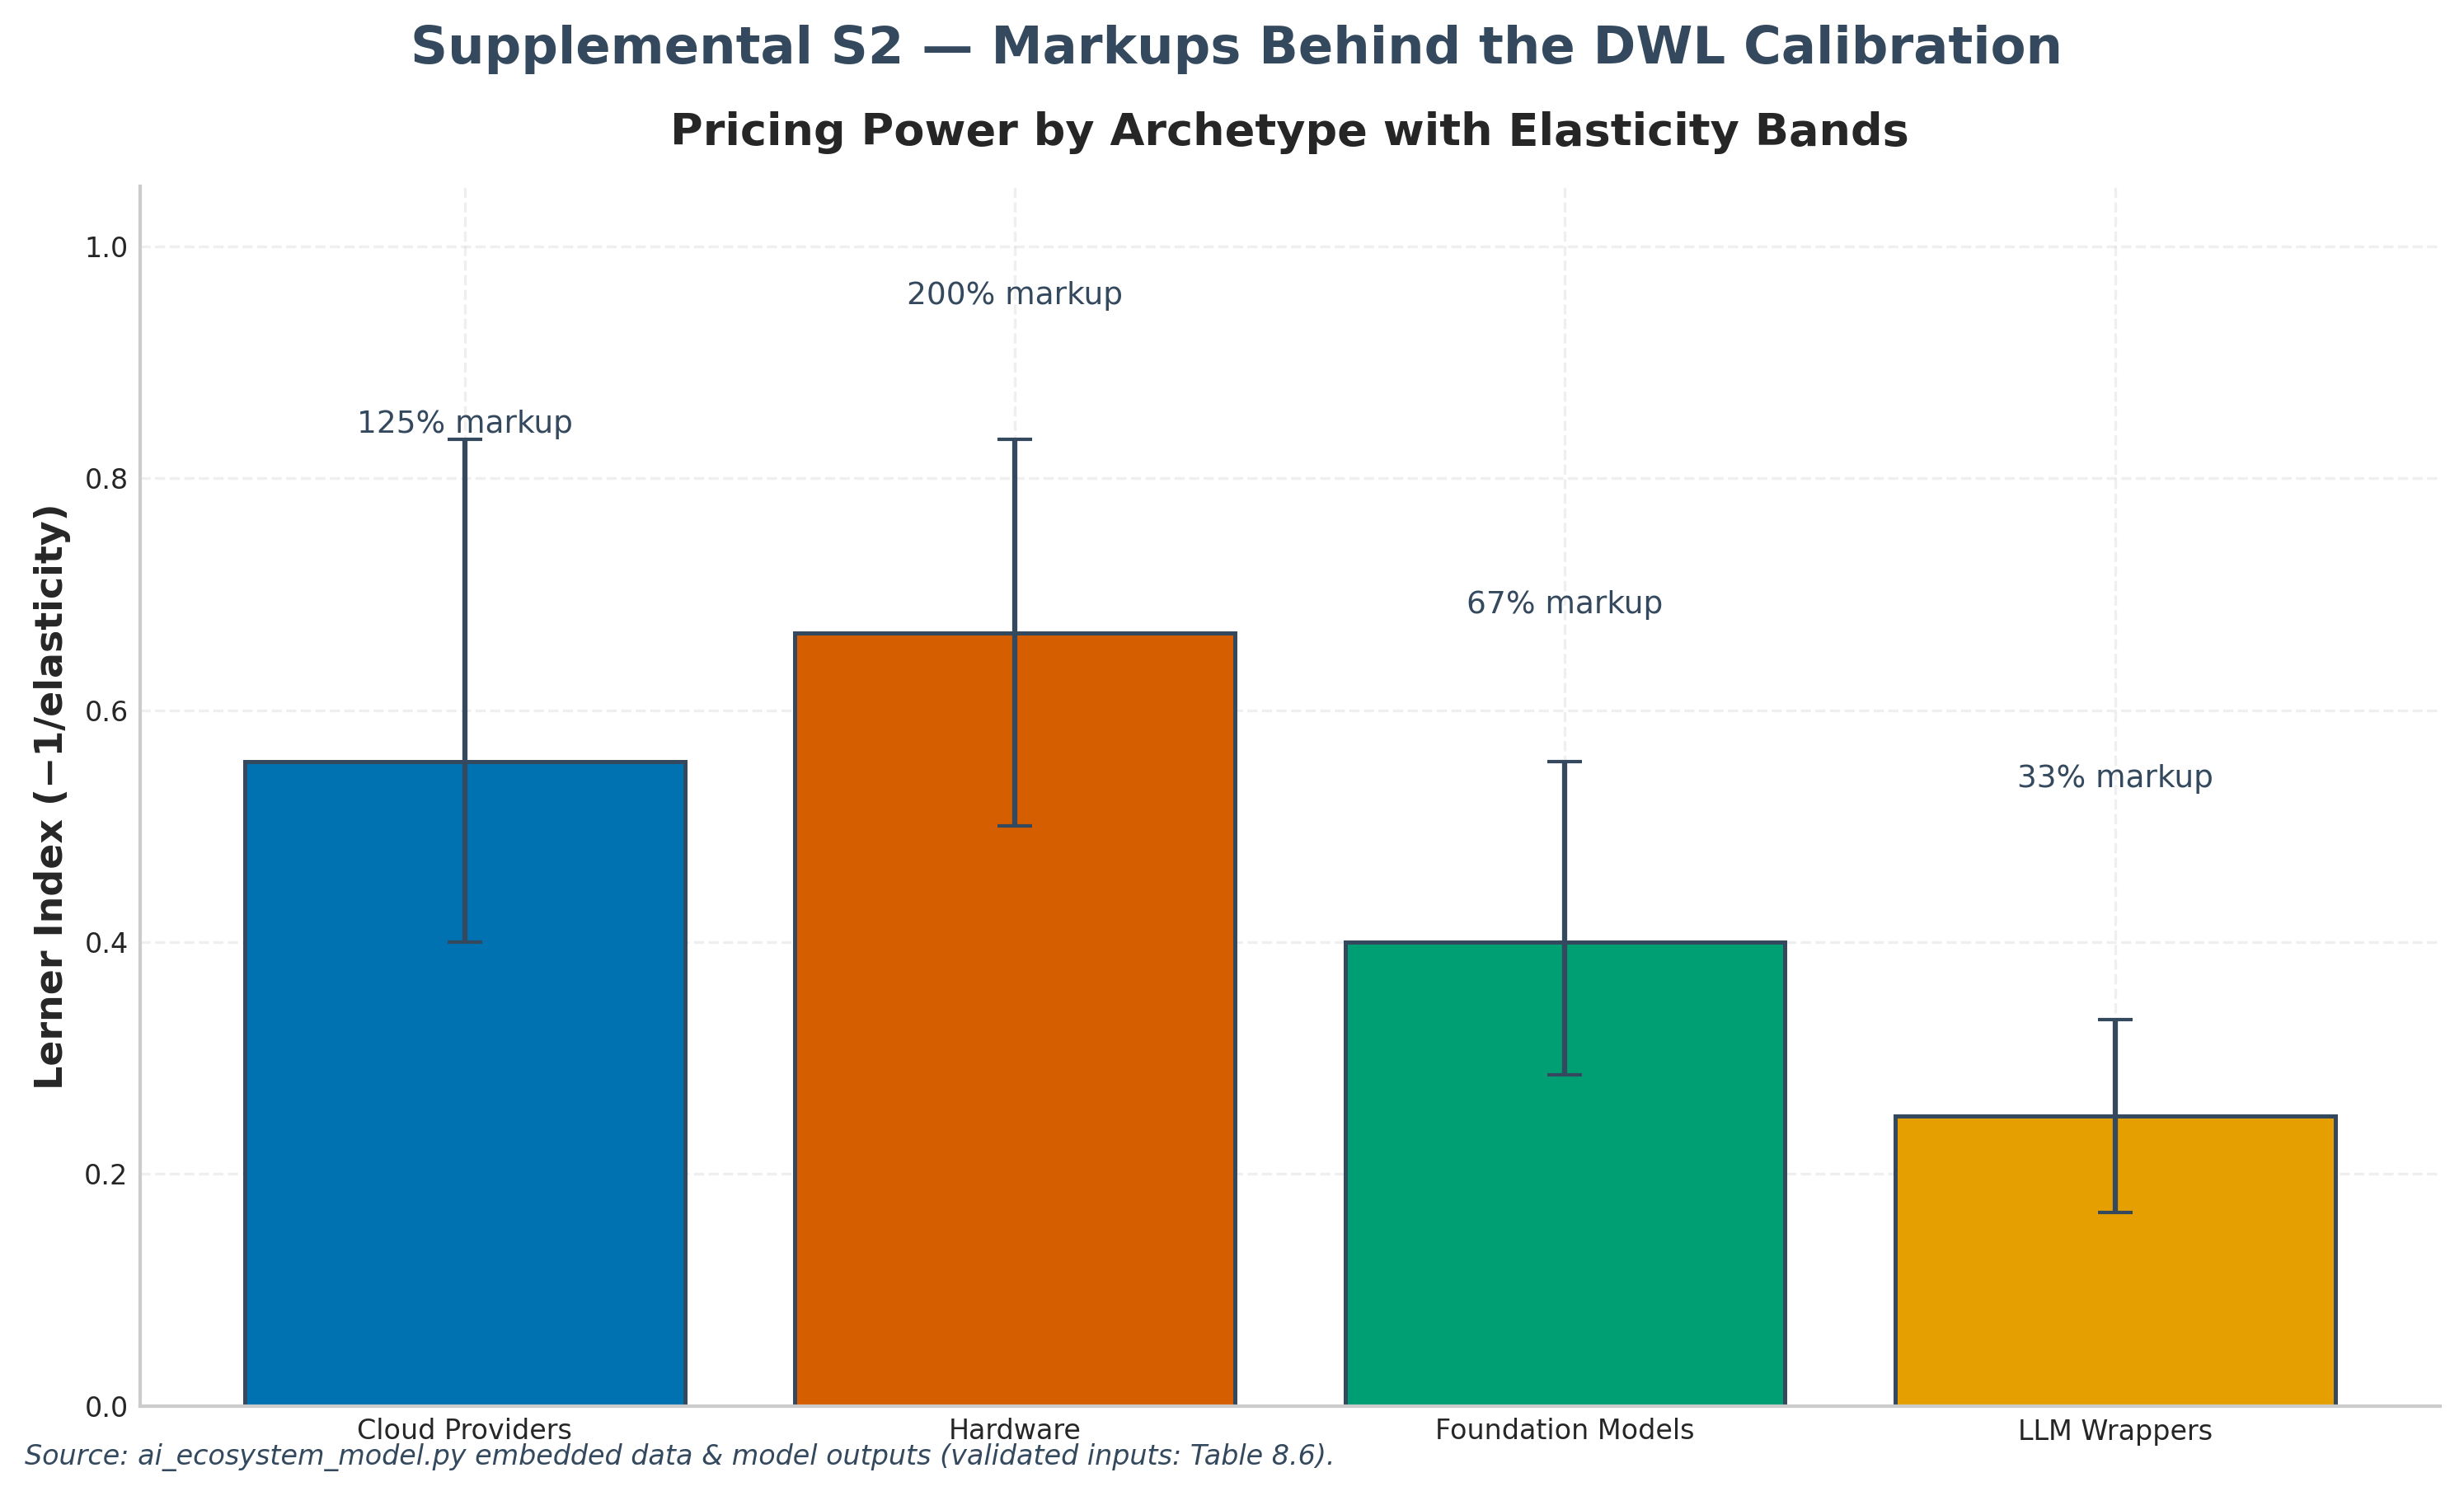
\includegraphics[width=0.9\textwidth,height=0.82\textheight,keepaspectratio]{supplemental/s2_lerner_markup_bands.png}
\caption{Market power behind the monopoly-pricing slice: Lerner indices with uncertainty bands (Table~7.17). Hardware's base markup of 200\% (band 100--500\%) and Cloud's 125\% show where the \$35.86B pricing distortion originates --- upstream, where the burst also lands.}
    \label{fig:09-market-power-behind-the}
\end{figure}

\begin{table}[htbp]
\centering
\caption{Waste by source (\$B). Order first, levels second.}
    \label{tab:04-waste-by-source-b}
\begin{tabular}{lr}
\toprule
Source & Loss \\
\midrule
Switching costs (lock-in) & 142.62 \\
Innovation distortion & 106.97 \\
Quality degradation & 71.31 \\
Coordination failures & 60.01 \\
Monopoly pricing & 35.86 \\
\midrule
\textbf{Total} & \textbf{416.77} \\
\bottomrule
\end{tabular}
\end{table}

\begin{figure}[htbp]
\centering
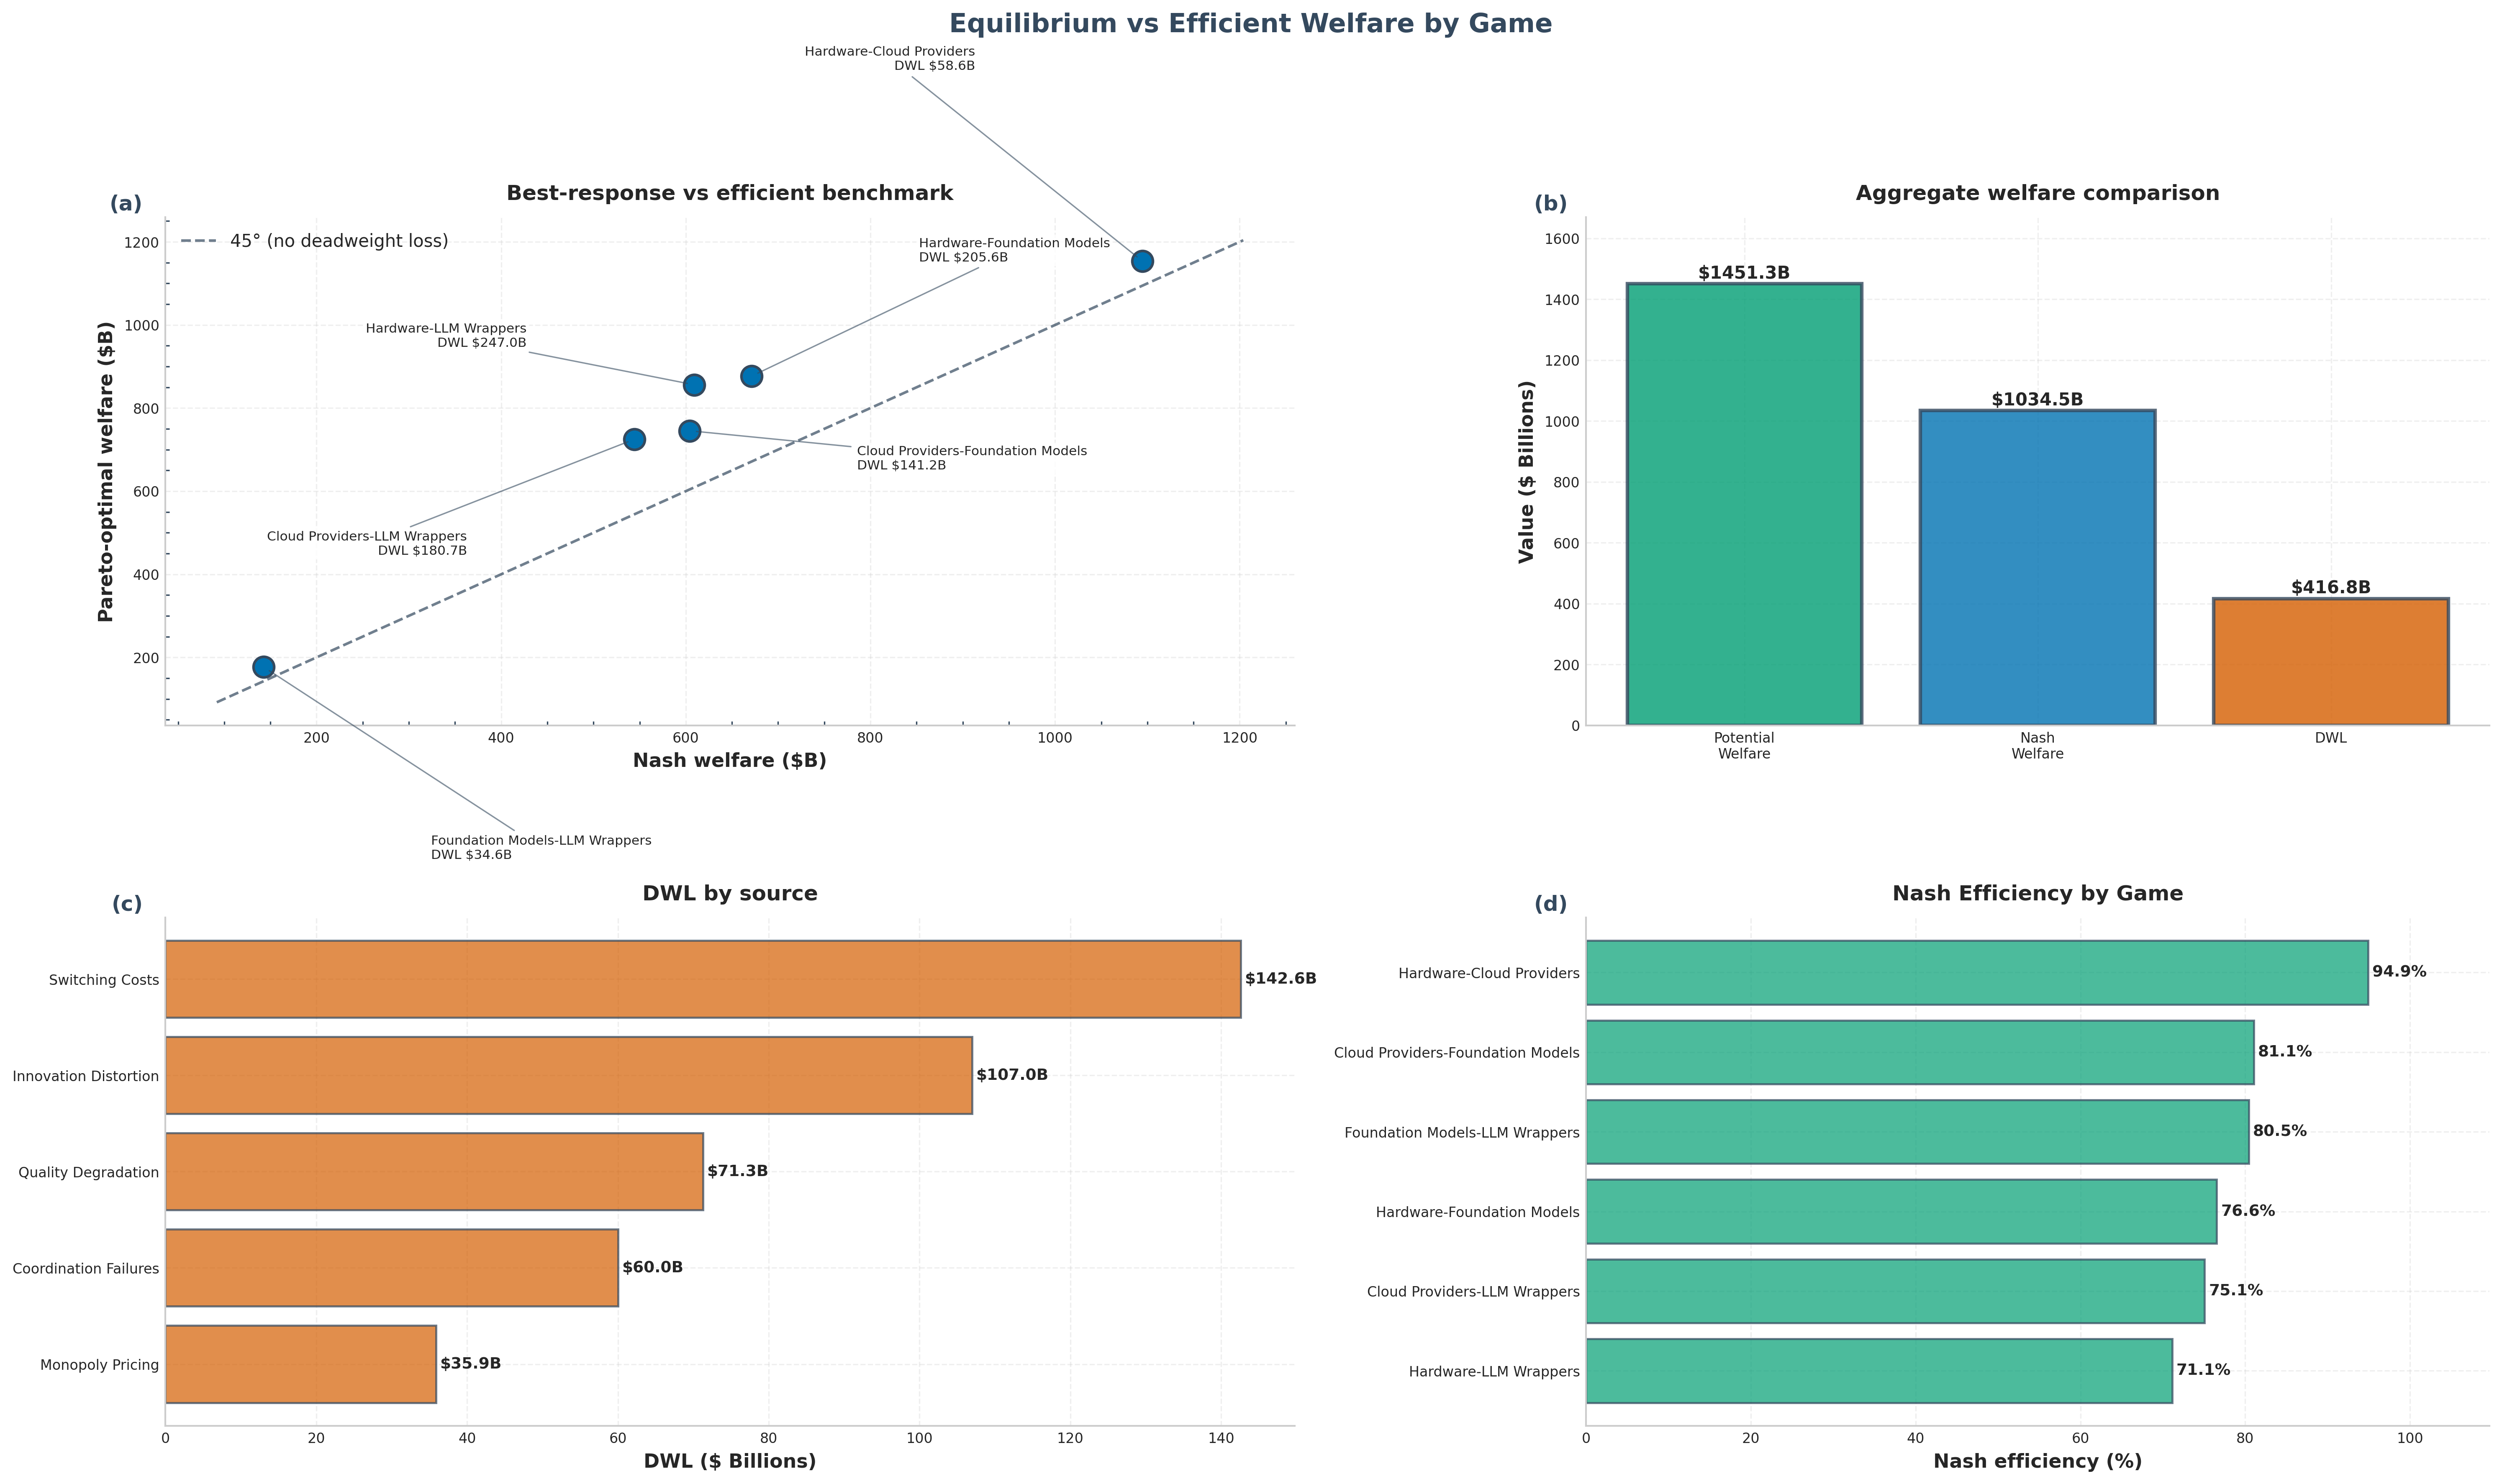
\includegraphics[width=0.9\textwidth,height=0.82\textheight,keepaspectratio]{figure_7.png}
\caption{Stuck versus best-joint outcomes by relationship: the gap is the waste, game by game. The core pair dominates, which is why one targeted remedy beats blanket platform rules.}
    \label{fig:02-stuck-versus-bestjoint-outcomes}
\end{figure}

\section{Bubble Vulnerability Assessment by Archetype}\label{sec:bubble}
Bubble-condition scores (vulnerability ratings from a scenario-calibrated
model, not measured probabilities; bands plotted below, drivers in the
\texttt{pred\_E} ledger) peak exactly where round-tripping is densest.

Prediction consequence: monitor frontier-lab funding rounds as the leading
indicator. Each mega-round at a higher valuation re-prices every adjacent
private mark at once. Anthropic at \$965B, Databricks near 905x earnings,
and xAI at 400x revenue have the furthest to fall.

\begin{figure}[htbp]
\centering
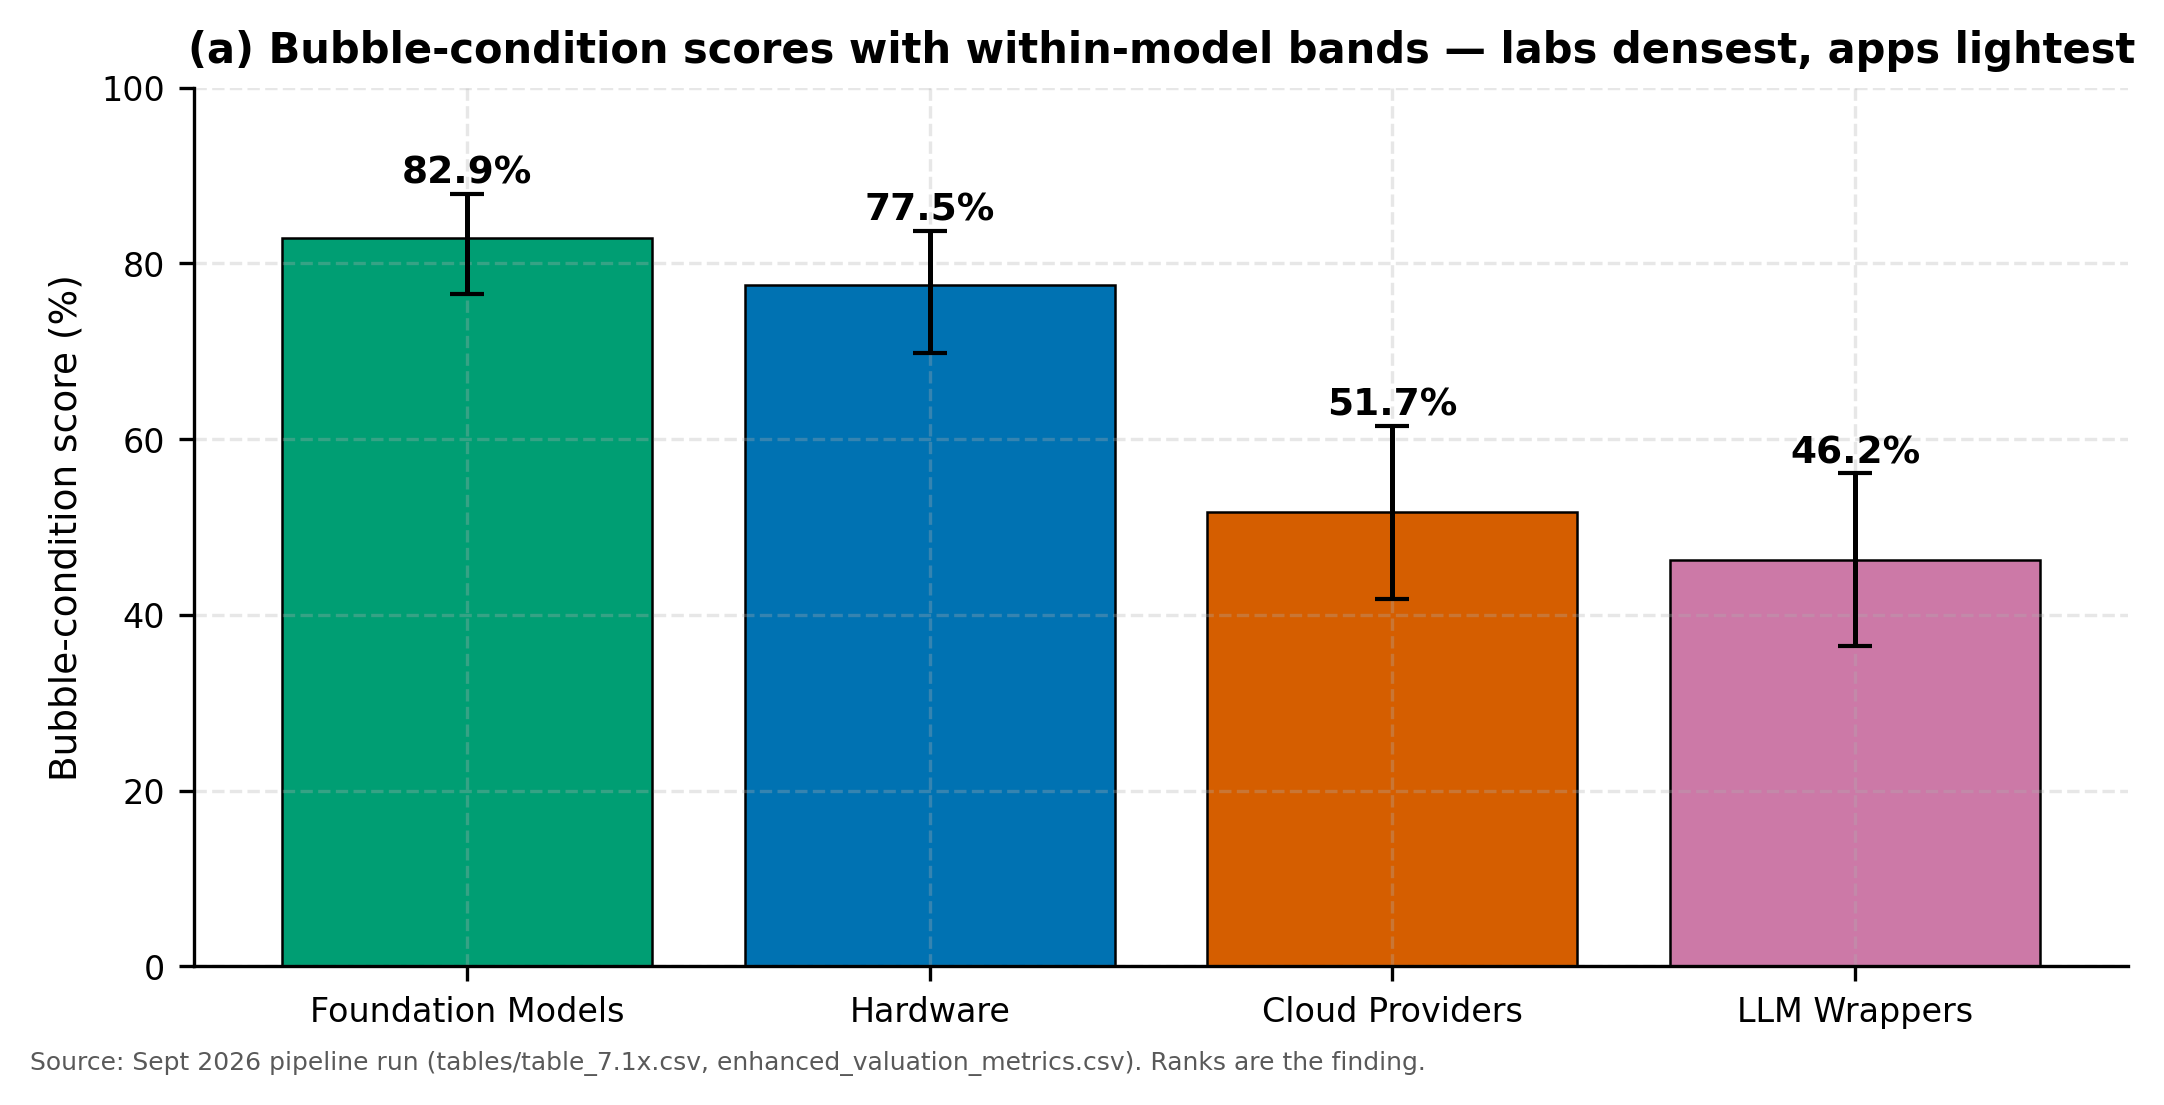
\includegraphics[width=\textwidth,height=0.82\textheight,keepaspectratio]{pred_formation_bands.png}
\caption{Bubble-condition scores with within-model robustness bands. The gap that matters is the top-two vs.\ bottom-two split: round-tripping density, not hype, separates them --- Wrappers carry maximum exuberance (1.0) yet score lowest (46.2\%) because their circular exposure is near zero (0.027).}
    \label{fig:10-bubblecondition-scores-with-withinmodel}
\end{figure}

\begin{table}[htbp]
\centering
\caption{Bubble-score driver decomposition (logit inputs; Table~7.10). Circular exposure dominates by construction (weight 1.6); exuberance alone cannot lift a score.}
    \label{tab:06-bubblescore-driver-decomposition-logit}
\begin{tabular}{lccccc}
\toprule
Archetype & Circ. & Capex & HHI sh. & Exub. & Score \\
\midrule
Foundation Models & 0.80 & 0.70 & 0.10 & 1.00 & 82.9 \\
Hardware & 0.40 & 0.90 & 0.46 & 0.83 & 77.5 \\
Cloud Providers & 0.23 & 0.60 & 0.40 & 0.09 & 51.7 \\
LLM Wrappers & 0.03 & 0.20 & 0.04 & 1.00 & 46.2 \\
\bottomrule
\end{tabular}
\end{table}

Driver reading: Hardware scores high on three of four pillars (capex 0.9,
HHI share 0.46, exuberance 0.83) but trails labs because its circular
exposure (0.40) is half theirs (0.80). Cloud scores lowest on exuberance
(0.09) --- its revenues are mostly non-AI --- which is why the credit
tripwire in Section~\ref{sec:contagion} starts at leveraged Cloud-adjacent names rather than
at the biggest clouds. Full driver ledger with bands: pipelines
\texttt{pred\_E\_formation\_drivers.csv}.

Uncertainty propagates three ways: stated bands ($z\pm0.4$) around the
weights, one-at-a-time quartering, halving, doubling and quadrupling (10/16 formation-order matches, 16/16 burst-order), and a 300-draw joint check
(seed 7) yielding formation-order exact-match 65\% ($\tau=0.88$,
Foundation Models top in 90\%) and burst-order exact match 100\%
($\tau=1.00$, Hardware first in all 300 draws). The specification gives
bubble-conditions probabilities of \textbf{82.9\%} for Foundation Models
(band 76.5--87.9), \textbf{77.5\%} for Hardware (69.8--83.7),
\textbf{51.7\%} for Cloud (41.8--61.5) and \textbf{46.2\%} for Wrappers
(36.5--56.1). These are scenario-calibrated vulnerability scores, not
empirically estimated event probabilities: no historical panel of
bubble/non-bubble episodes exists to calibrate against, so the bands
quantify within-model robustness, not statistical confidence. The weights
carry structurally identified intervals (Table~8.7) rather than pure
judgment --- the formation order pins the capex weight to a two-sided
\AeightCapex{} and the concentration weight to \AeightHhi{}, while the
circularity weight admits \AeightCirc{} and the exuberance weight
\AeightExub{} ($+$ marks an edge extending beyond the searched range).

A second, independent screen agrees. The five-pillar classification (Table~7.7,
built from narrative tilt, multiple exuberance and expansion, circular-hype
proxies, and capex intensity rather than the formation logit) labels
Foundation Models the stack's sole ``Bubble risk'' (0.507), Hardware and
Wrappers ``Boom'' (0.408, 0.352), and Cloud plain ``Buildout'' (0.317).
Two different machines, same verdict on who is most fragile --- which is
what lets P5 in the registry hold at $\sim$60\% despite the formation rank's
weaker 65\% joint record. Fragility and instability coincide --- labs and
apps score lowest on stability (0.38, 0.12) while infrastructure scores
highest (0.78, 0.75) --- yet the burst order runs opposite: what breaks
first in funding order breaks last in dollar order.

\begin{figure}[htbp]
\centering
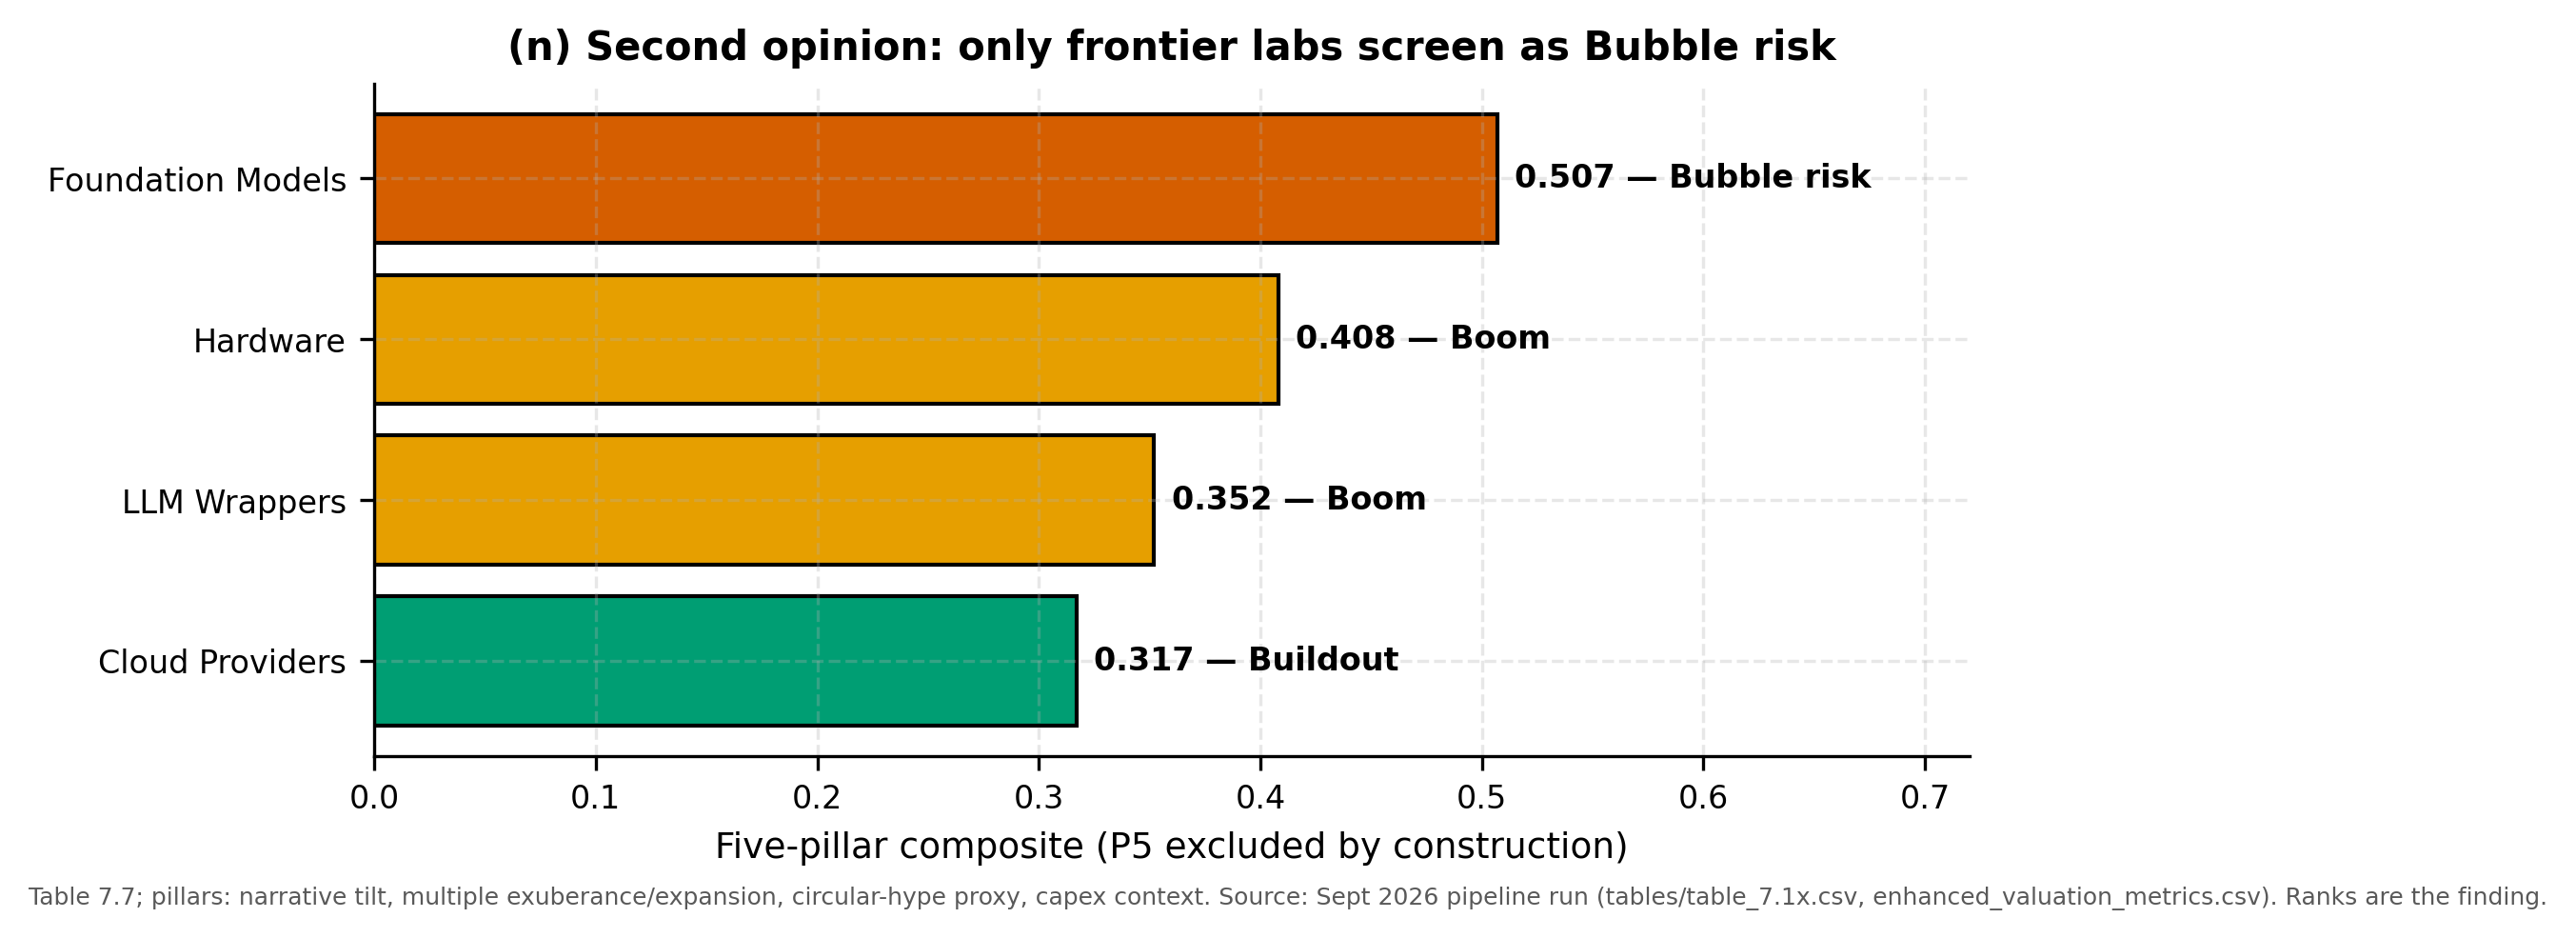
\includegraphics[width=\textwidth,height=0.82\textheight,keepaspectratio]{pred_five_pillar.png}
\caption{Five-pillar screen (Table~7.7): the independent second opinion. Only frontier labs clear the ``Bubble risk'' bar; Cloud scores lowest as plain ``Buildout.'' Agreement between two differently built screens is worth more than precision in either one.}
    \label{fig:12-fivepillar-screen-table77-the}
\end{figure}

\begin{figure}[htbp]
\centering
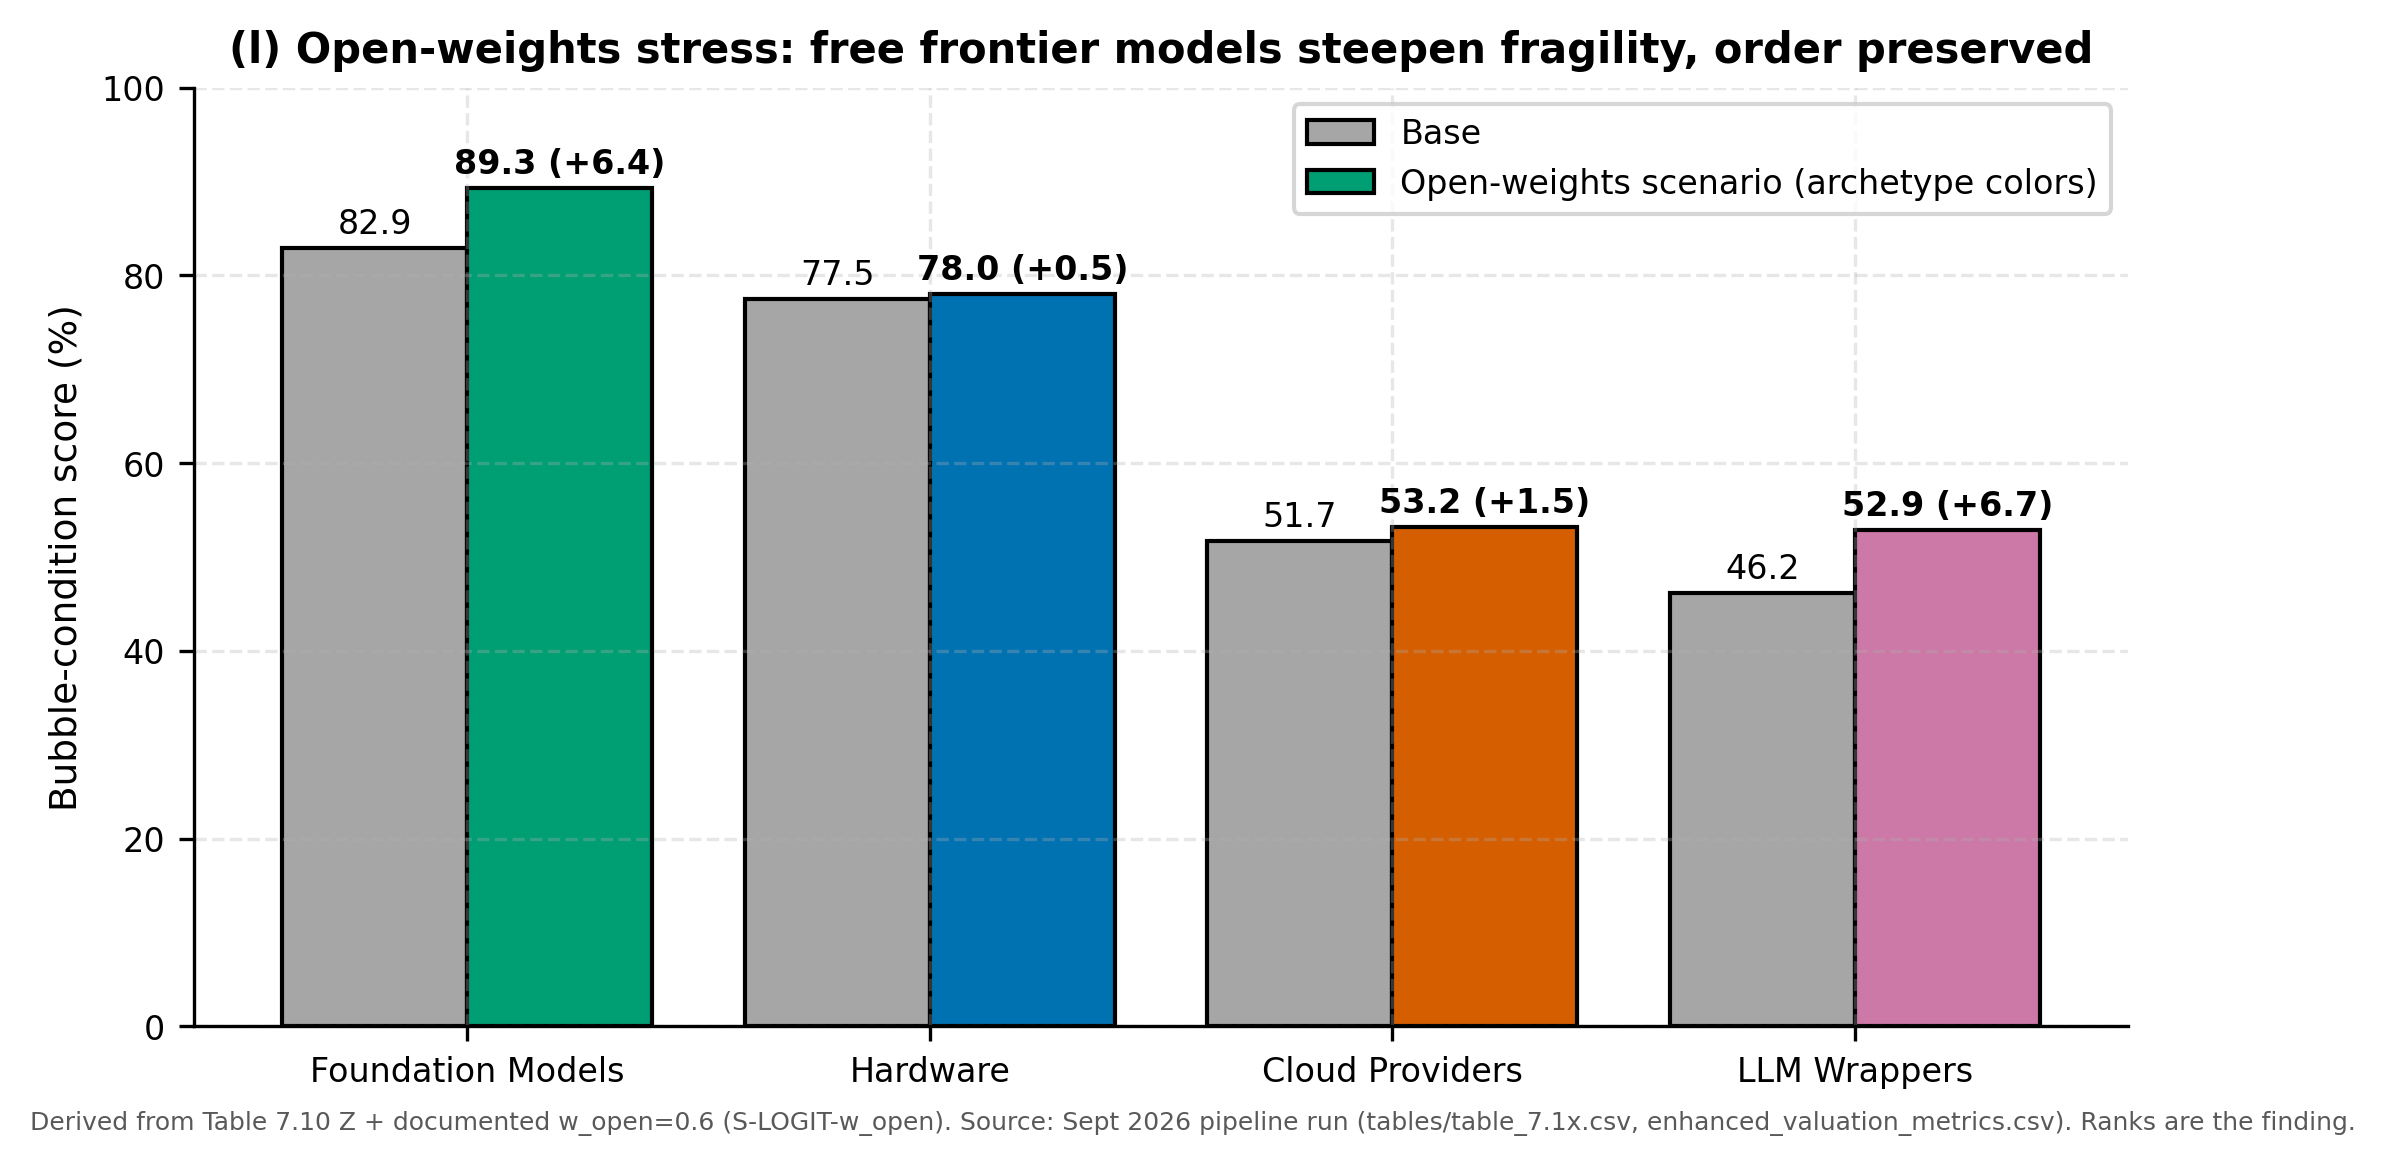
\includegraphics[width=\textwidth,height=0.82\textheight,keepaspectratio]{pred_open_weights.png}
\caption{Open-weights stress scenario (validated S-LOGIT-w\_open channel --- the open-weights term in the formation logit): free frontier models compress lab and wrapper margins, steepening formation scores --- labs 82.9\% to 89.3\%, wrappers 46.2\% to 52.9\% --- while the rank order is preserved. The thesis steepens rather than breaks: inference still runs on bought silicon.}
    \label{fig:13-openweights-stress-scenario-validated}
\end{figure}

Both screens corroborate the
registry; neither changes its likelihoods.

\section{Burst Incidence: Loss Ranking, Severity, and Macroeconomic Transmission}\label{sec:burst}
A severe scenario (70\% of circular capital impaired, 30\% AI-capex cut)
destroys value in the reverse order of the hype:

\begin{table}[htbp]
\centering
\caption{Severe-burst destruction by archetype (\$B): Hardware \$239.4B (50.1\%), Cloud \$132.7B (27.7\%), labs \$85.4B (17.9\%), Wrappers \$20.8B (4.4\%); shares sum to 100.1\% on rounding.}
    \label{tab:08-severeburst-destruction-by-archetype}
\begin{tabular}{lcr}
\toprule
Archetype & Loss & Rank \\
\midrule
Hardware & 239.4 & 1 \\
Cloud Providers & 132.7 & 2 \\
Foundation Models & 85.4 & 3 \\
LLM Wrappers & 20.8 & 4 \\
\midrule
\textbf{First-round total} & \textbf{478.3} & \\
Second reverberation round & 15.2 & \\
\bottomrule
\end{tabular}
\end{table}

The ranking is the most stress-tested claim in this paper: 16 of 16
one-at-a-time extremes, 100\% agreement across 300 joint draws, Hardware
first every time, replicated across seeds and noise screens. It holds
because inference still runs on someone's silicon and someone's cloud no
matter whose logo is on the model.

Direct-vs.-network split adds a second prediction inside the ranking:
Hardware's loss is 56\% direct (\textasciitilde\$133B of \$239.4B) --- it owns the
impaired contracts --- while Wrappers' loss is 97\% network (\$20.16B of
\$20.83B): apps are pure contagion victims with almost no direct exposure
(\$0.67B). Cloud splits evenly (\$67.85B direct, \$64.85B network); labs lean
direct (\$59.64B vs.\ \$25.75B). A burst that spares Hardware's contract book
but hits app revenues would flip the Wrappers row without moving the top
two --- one more reason the ranking's head is sturdier than its tail.

The valuation-vs.-contract paradox is the point, not a puzzle: frontier
labs score highest on bubble vulnerability (82.9\%) because private marks
detached furthest from revenue, yet Hardware absorbs the largest dollar
hit because it holds the contracts, the guarantees, and the capex. Screens
built on multiples would aim at the labs; the money says aim at the
toolmakers.

\begin{figure}[htbp]
\centering
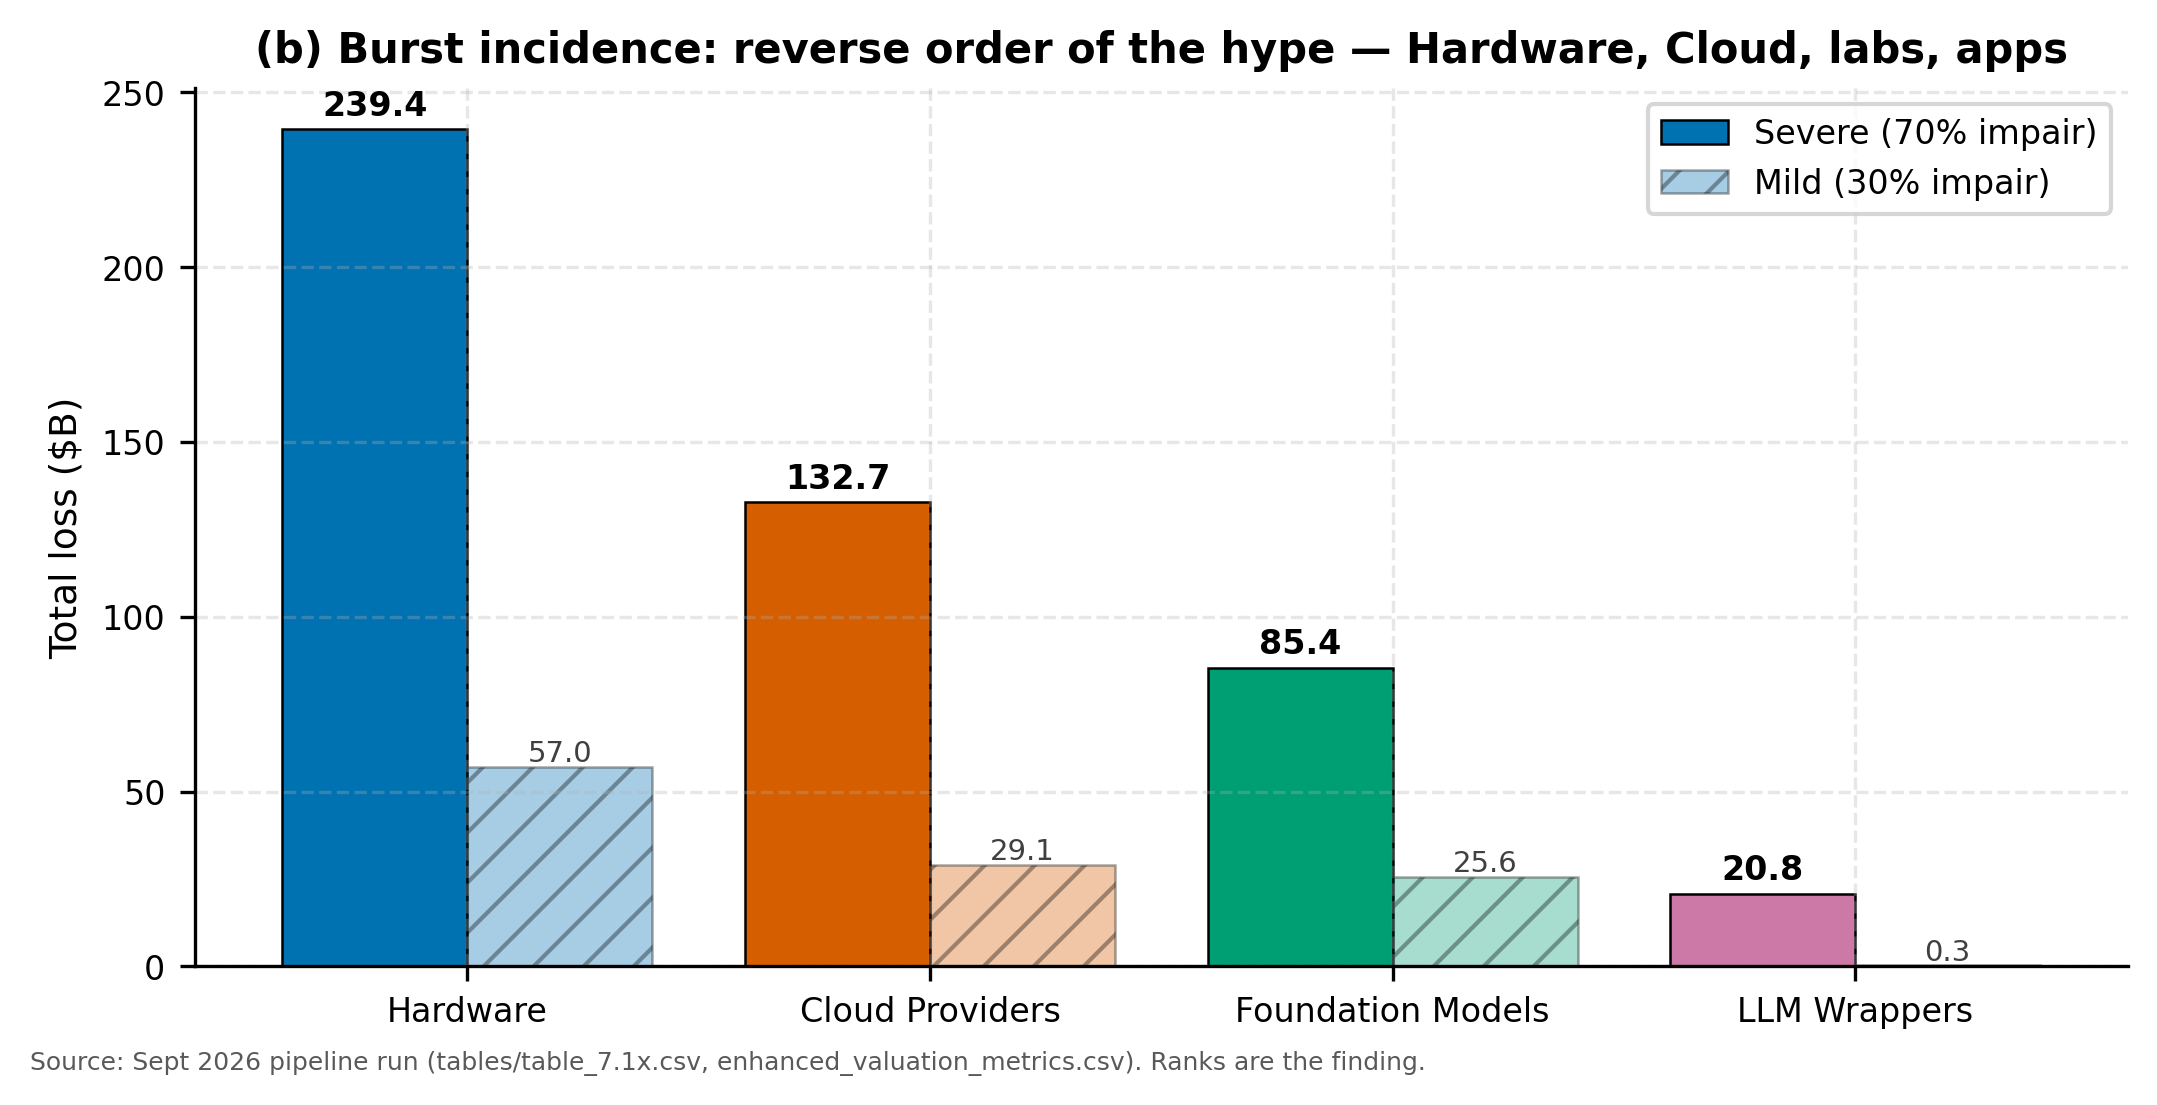
\includegraphics[width=\textwidth,height=0.82\textheight,keepaspectratio]{pred_burst_waterfall.png}
\caption{Severe vs.\ mild burst losses by archetype. Severity scales levels roughly 4x; the order never changes --- the visual equivalent of the 16/16 stress result.}
    \label{fig:14-severe-vs-mild-burst}
\end{figure}

\begin{figure}[htbp]
\centering
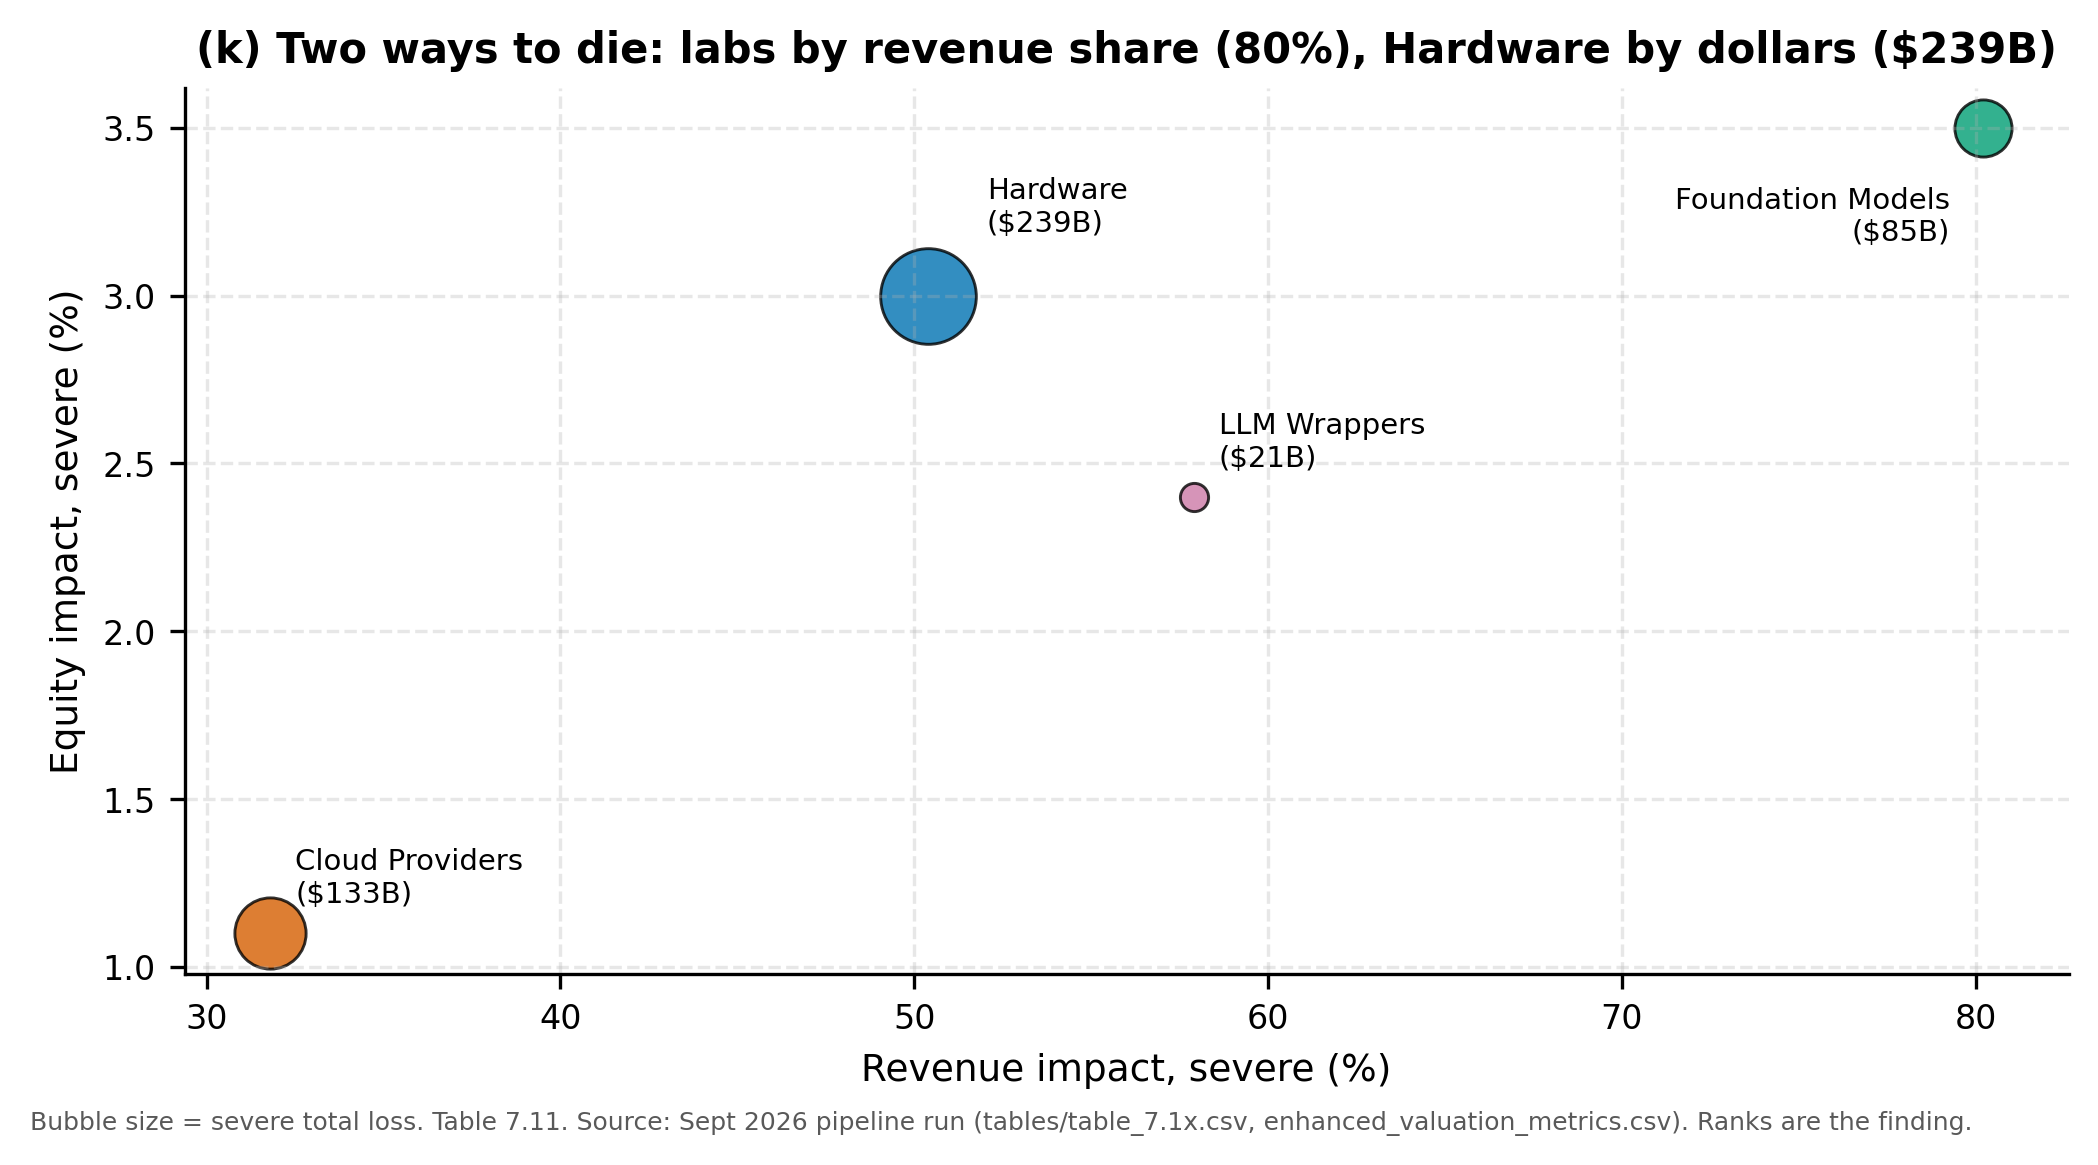
\includegraphics[width=\textwidth,height=0.82\textheight,keepaspectratio]{pred_equity_revenue_impact.png}
\caption{Two dimensions of pain (Table~7.11): revenue share destroyed vs.\ equity value destroyed, sized by dollar loss. Frontier labs face an 80.2\% revenue hit but only \$85B in dollars; Hardware loses \$239B at a 50.4\% revenue hit. Short the multiple where revenue evaporates; hedge the dollars where contracts break.}
    \label{fig:15-two-dimensions-of-pain}
\end{figure}

\begin{figure}[htbp]
\centering
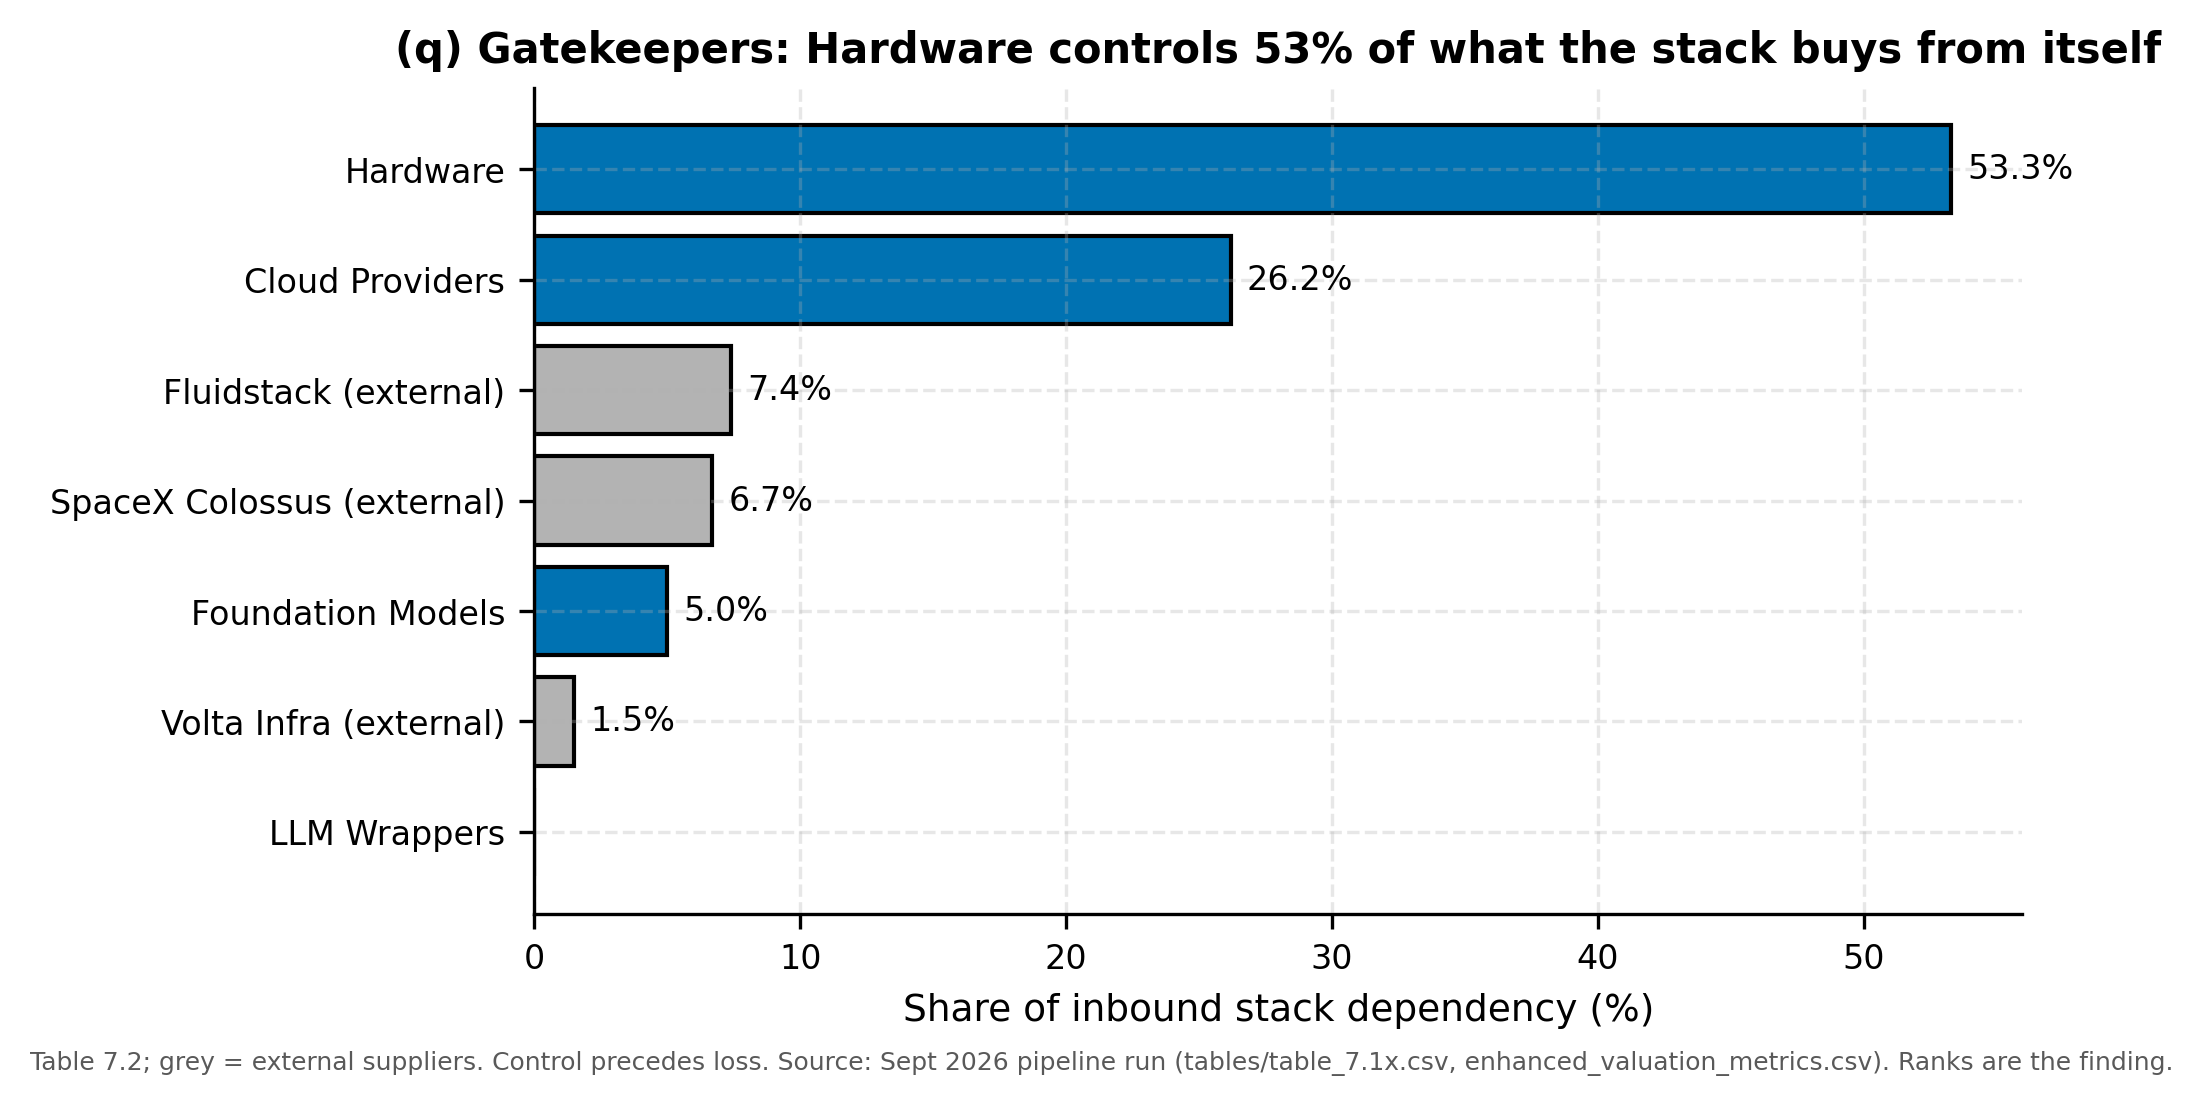
\includegraphics[width=\textwidth,height=0.82\textheight,keepaspectratio]{pred_gatekeeper.png}
\caption{Gatekeeper shares (Table~7.2): who controls what the stack buys from itself. Hardware gates 53.3\%, Cloud 26.2\%, frontier labs only 5.0\% --- control precedes loss, so the burst order follows the gatekeeper order. Grey bars are external suppliers (Fluidstack, Colossus, Volta).}
    \label{fig:16-gatekeeper-shares-table72-who}
\end{figure}

\emph{When, not just how much.} Formation scores convert into a burst-timing
window under a stated quarterly hazard: hazard equals formation probability
divided by a 12-quarter formation-to-burst lag (the 2005--2008 and
1999--2002 vintages both run about three years from dense formation to
burst), with median quarters to burst $\ln(2)/h$. The first-tip system clock
reads a median of 10.0 quarters from the September 2026 vintage (Q2'29),
set by Foundation Models at the same horizon; Hardware follows at
10.7 quarters (Q3'29), Cloud at 16.1 (Q4'30), Wrappers at 18.0 (Q2'31).
The honest uncertainty is the lag, not the band: varying it over 8--20
quarters spans Q3'28--Q1'31 at the system level, while the formation band
barely moves the median. Scenario arithmetic, not a forecast: move the
stated lag and every quarter moves with it. Machine-readable:
\texttt{pred\_G\_burst\_timing.csv}.

\begin{figure}[htbp]
\centering
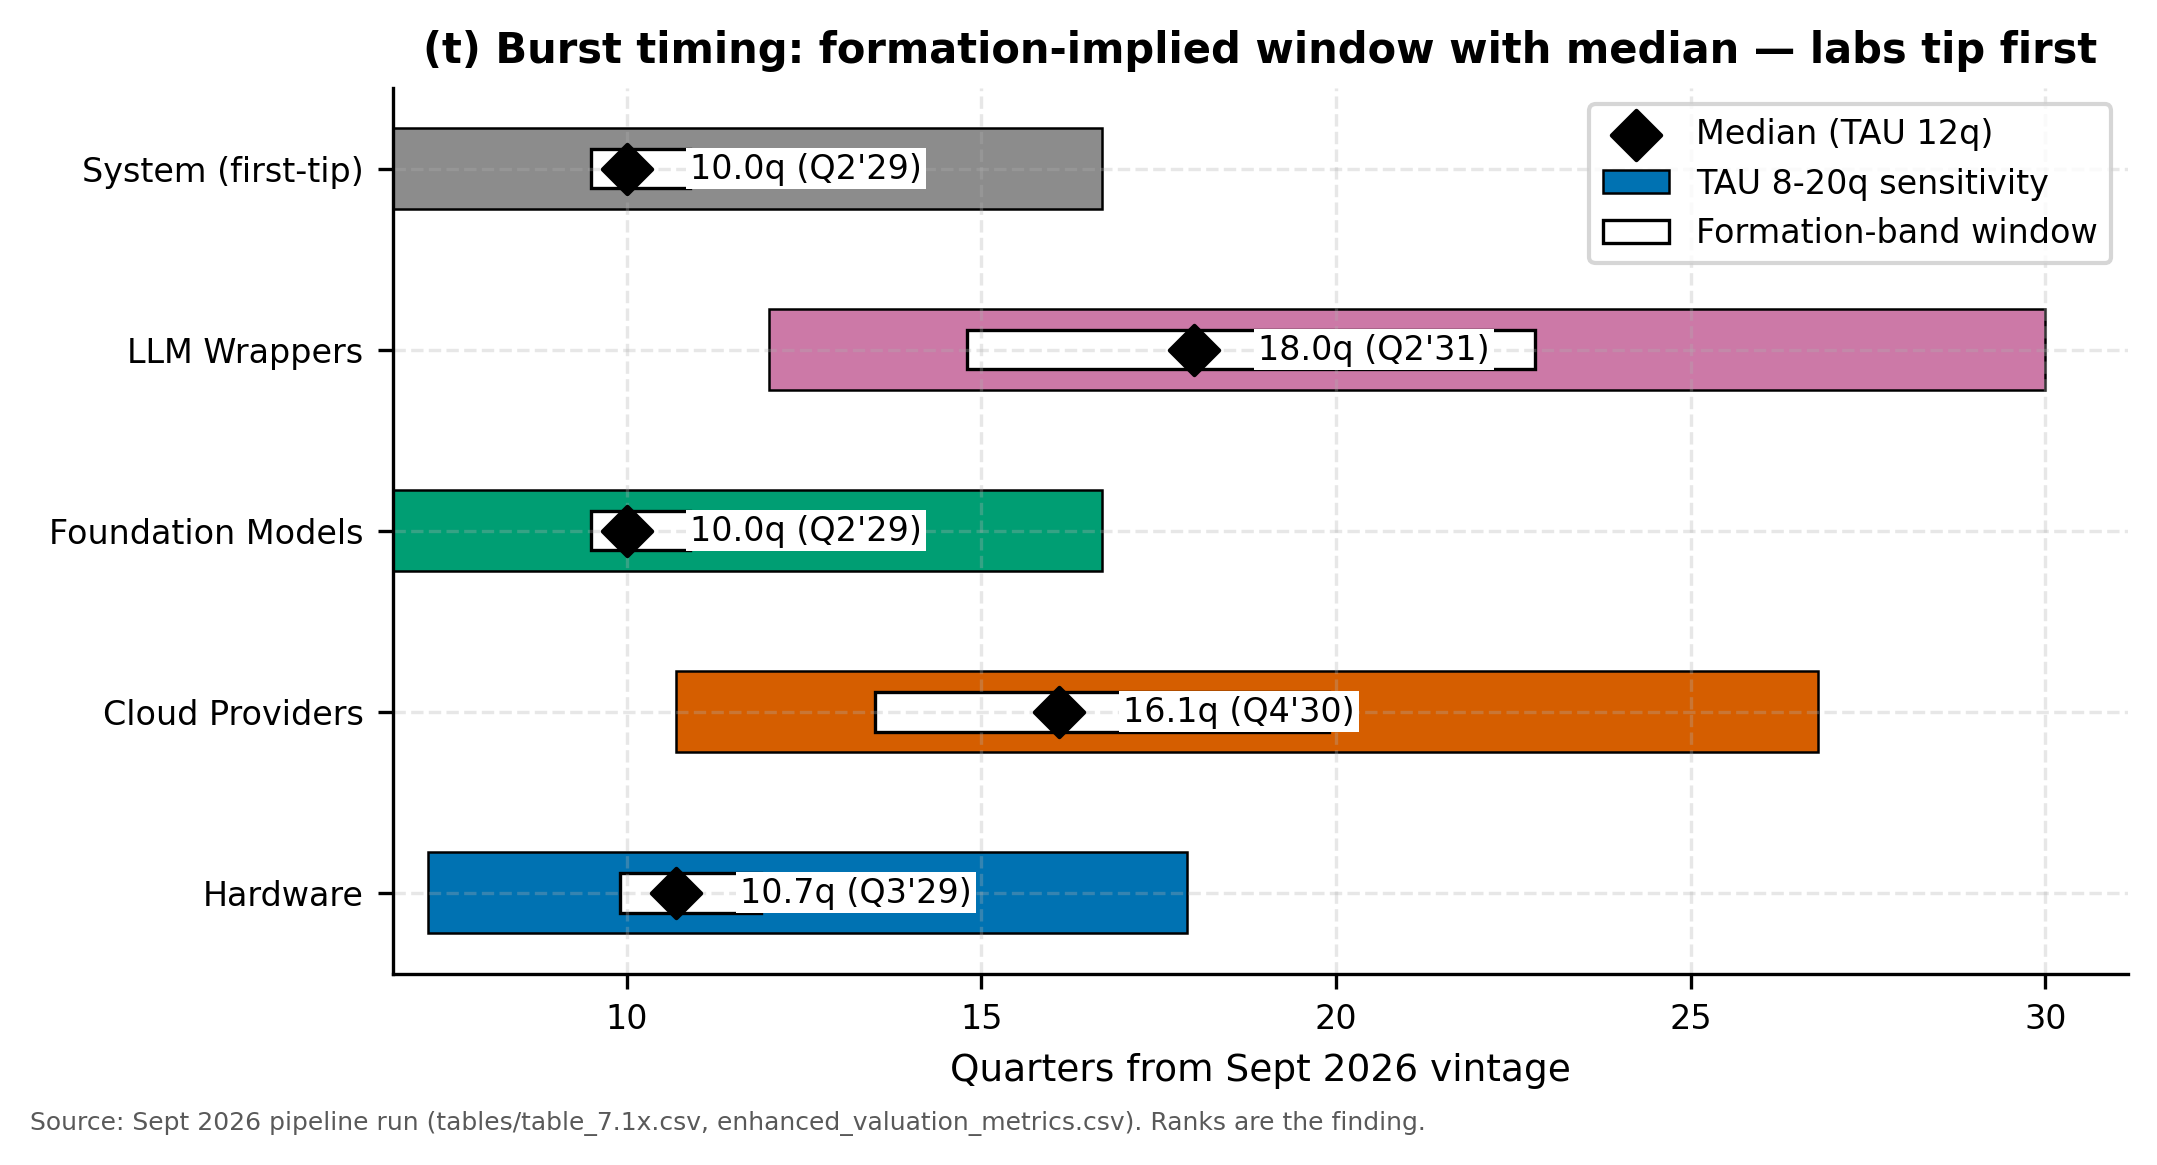
\includegraphics[width=\textwidth,height=0.82\textheight,keepaspectratio]{pred_timing_window.png}
\caption{Hazard-implied burst windows from the September 2026 vintage. Thick bars span the 8--20-quarter lag sensitivity, white insets the formation band, diamonds the base-lag median. Foundation Models tip first; the system clock follows them into Q2'29.}
    \label{fig:burst-timing-window}
\end{figure}

\emph{Why this timing, and what would change it.} The 10.0-quarter base is a
hazard clock, not a date prediction (P8 stays unassigned): formation
probability over a stated 12-quarter lag, nothing more. Conditioning that
clock on September-2026 evidence gives a conditional call at a median of 11.0 quarters (Q3'29), window Q4'28--Q2'31. The
why-ledger decomposes the call by weight (machine-readable:
\texttt{pred\_L\_timing\_rationale.csv}).
\emph{High:} the hazard base itself --- Foundation Models at 82.9\%
formation times the stated lag. \emph{Medium, +1 quarter:} trigger
conditioning --- no \texttt{pred\_B} tripwire reads tripped on price
evidence (hazard Low on NVDA/QQQ/SPY at 8/7/16), a stated calm credit,
flagged as judgment rather than measurement. \emph{Medium, +0:} gauge
triangulation --- NVDA's convex-max of 3.6 fires while its hazard stays Low,
against 9.9 with hazard 100 at the March-2000 top and 2.9 with hazard 60 at
the October-2007 top: acceleration without stress, so no pull-forward.
\emph{Low, +0:} precedent topping lag --- the 2000/2007 tops preceded
crash-week clusters by 2--8 quarters, which supports the window width, not
the median. What breaks the call is stated alongside it: any
\texttt{pred\_B} tripwire tripping revokes the +1Q credit (median back to
10.0Q), and a hazard-regime flip to High on live names would pull it
forward further. Sensitivity on the one judgment: no credit gives the base, double credit reaches median 12.0q (Q4'29).

\begin{figure}[htbp]
\centering
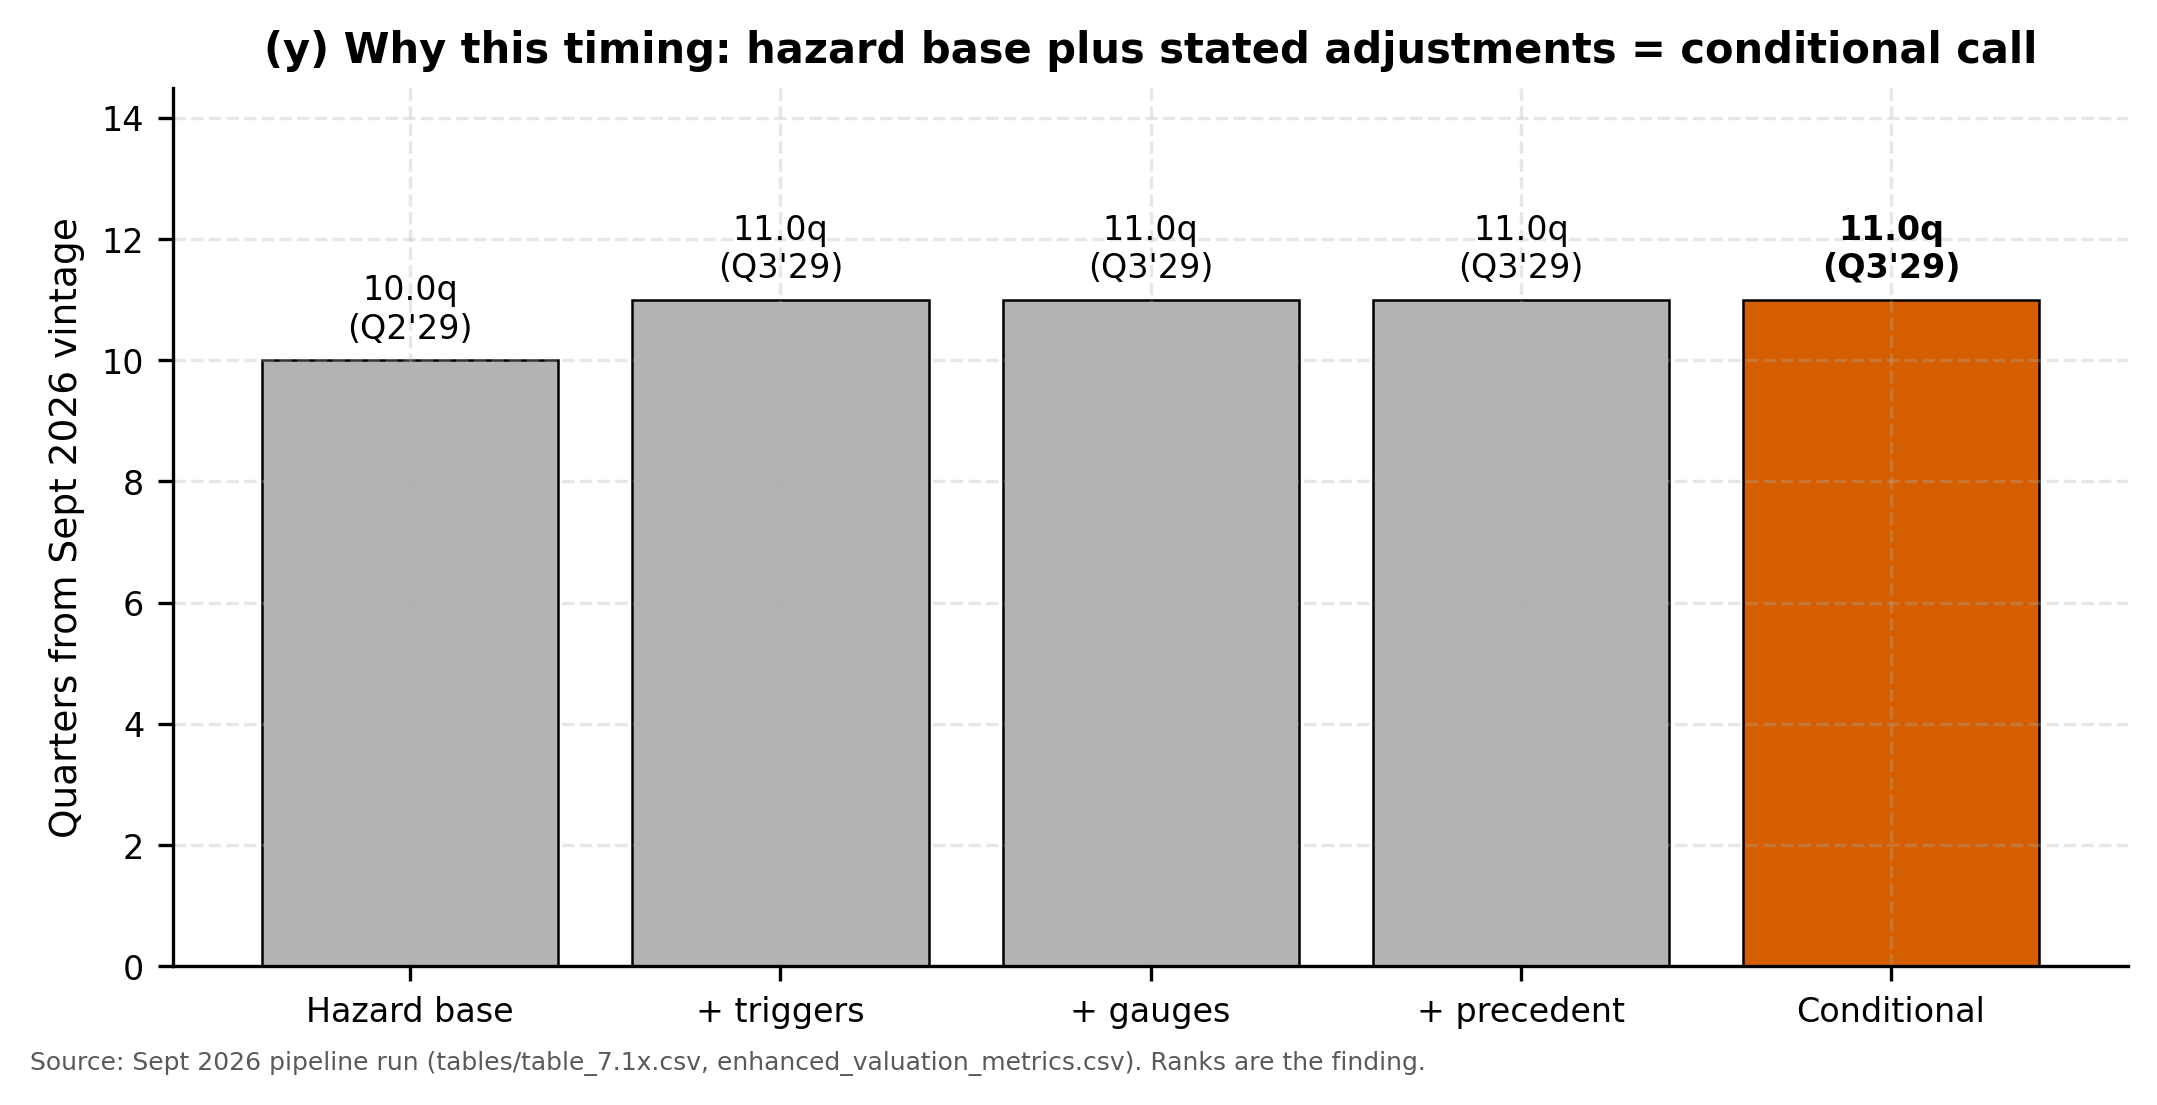
\includegraphics[width=\textwidth,height=0.82\textheight,keepaspectratio]{pred_timing_call.png}
\caption{From hazard base to conditional call. The +1Q trigger calm-credit is the only judgment in the bridge; gauges and precedent add nothing. If a tripwire trips, the call falls back to the 10.0Q base.}
    \label{fig:timing-conditional-call}
\end{figure}

Within-layer concentration (Table~7.1b) rules out the comforting story that
any single archetype is internally competitive: every layer screens
``highly concentrated'' (HHI 4,057--5,632), with the frontier-lab duo most
concentrated of all (5,283, Anthropic 61.9\%). There is no diversified
corner of the stack to hide in --- which is why the burst ranking is an
address book, not a hedge.

GDP transmission runs through two channels calibrated to US GDP
(\$30,767.1B): canceled tech investment (\$120.0B severe; \$40.0B mild) and
the equity-wealth effect at 4 cents on the dollar (\$19.1B severe; \$8.2B
mild) --- combined severe cost \$139.1B (0.452\% of GDP), mild \$48.2B
(0.157\%), no multiplier. The 4-cent calibration is the \citet{carroll2011}
financial-wealth estimate, corroborated by local labor-market evidence on
stock-wealth spending effects \citep{chodorowreich2021}. The capex channel
dominates in both states
(86\% severe, 83\% mild); wealth adds $\sim$\$4B per \$100B destroyed.
Portable rule: each \$100B of destroyed AI value
drags $\sim$\$4B of GDP through household wealth, plus the local capex-cut
share. Who holds that wealth loss --- and at what propensity to consume ---
is a retirement story told in the Online Appendix: the
uniform 4-cent assumption overstates the aggregate drag while understating
its concentration on 401(k) and pension holders. The Online Appendix sizes
the exposed base at $\sim$\$2.9T of Big Tech equity at a 34\% index weight
(ICI Q2-2026 levels, a market-weight floor): the aggregate 0.452\% drag is
small, but its incidence concentrates on near-retirement cohorts whose
defined-contribution balances overweight the names that fall first.

\begin{figure}[htbp]
\centering
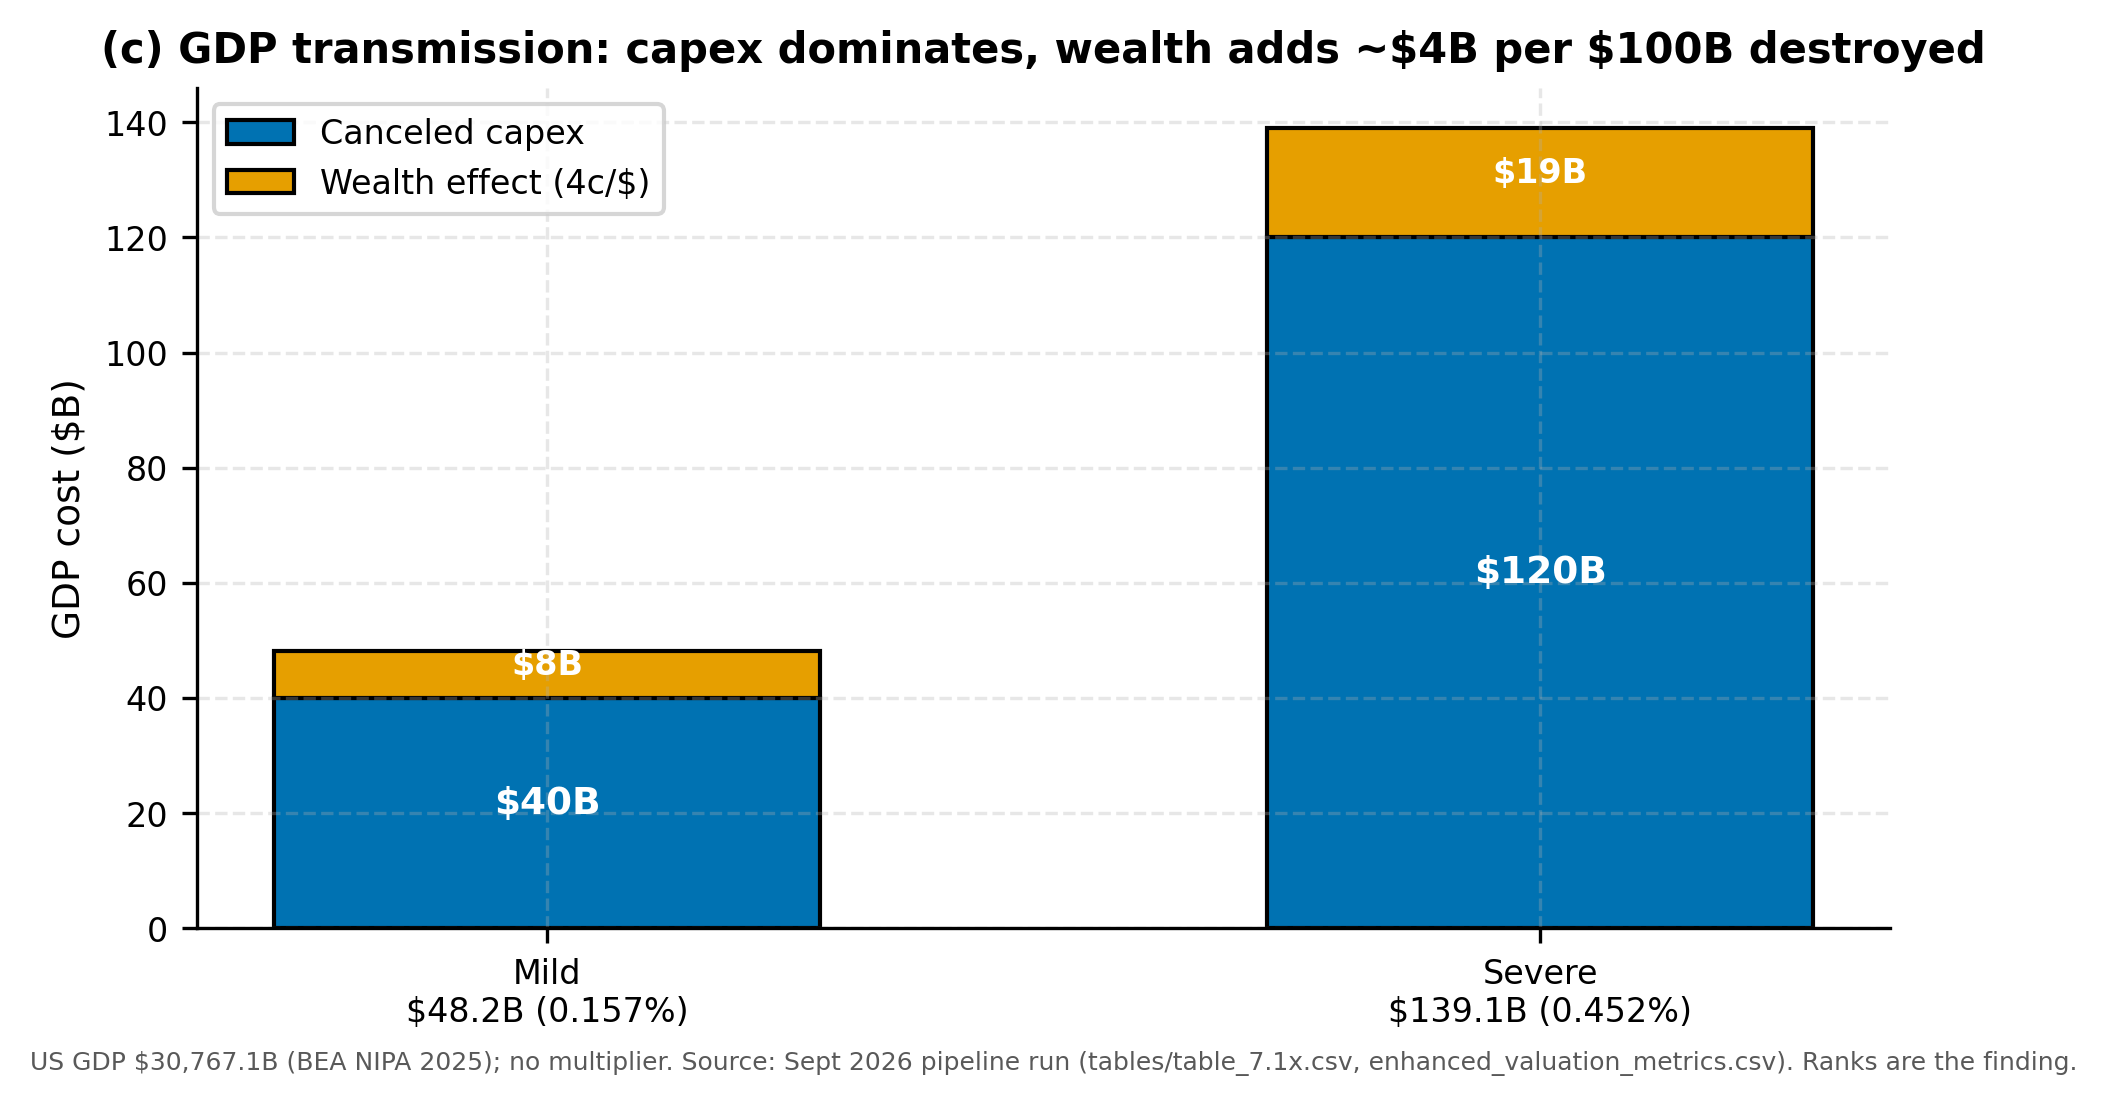
\includegraphics[width=0.9\textwidth,height=0.82\textheight,keepaspectratio]{pred_gdp_waterfall.png}
\caption{GDP transmission stacked: canceled capex (dark) plus the 4-cents-on-the-dollar wealth effect (light). Both scenarios are capex stories with a wealth footnote.}
    \label{fig:17-gdp-transmission-stacked-canceled}
\end{figure}

\begin{figure}[htbp]
\centering
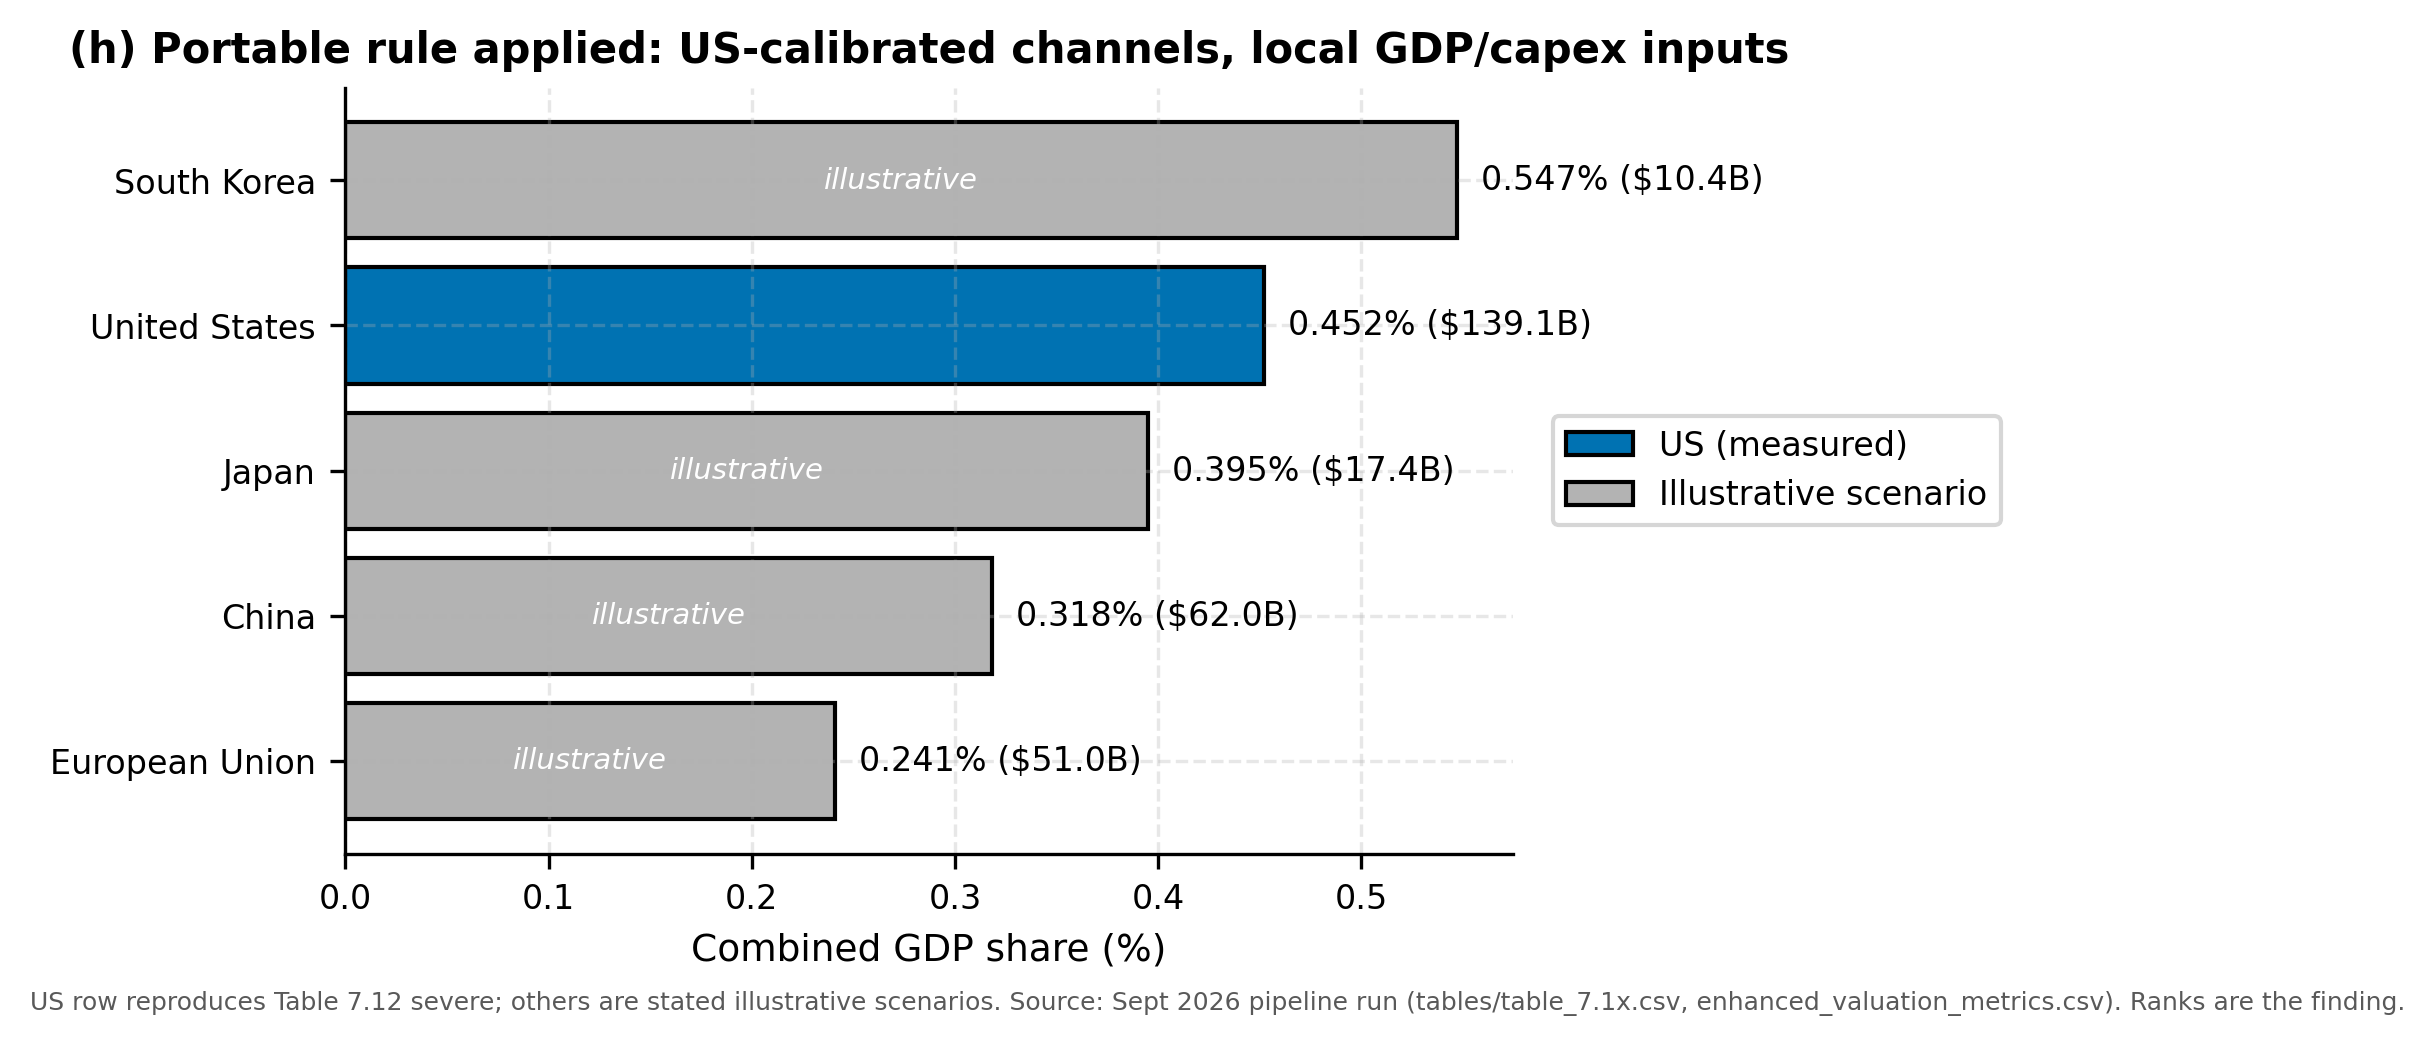
\includegraphics[width=\textwidth,height=0.82\textheight,keepaspectratio]{pred_geography_bars.png}
\caption{Portable transmission rule applied to other economies (Table~7.19). Only the US row reproduces a calibrated estimate; the rest are stated illustrative scenarios (30\% capex-cut severity, no multiplier) for readers to replace with local vintages. Korea's 0.547\% share leads because its GDP base is smallest against an illustrative capex-heavy input --- a composition effect, not a forecast.}
    \label{fig:03-portable-transmission-rule-applied}
\end{figure}

Table~7.19 runs the first porting: the United States row reproduces the
default calibration (\$139.1B, 0.452\%), and four stated illustrative
scenarios apply the same severity abroad --- European Union \$51.0B
(0.241\%), China \$62.0B (0.318\%), Japan \$17.4B (0.395\%), South Korea
\$10.4B (0.547\%) --- each flagged Illustrative=Y with its GDP vintage and
scenario inputs shown as explicit columns. GDP vintages are World Bank WDI
2025 (European Union, China, Japan, South Korea) and BEA NIPA
(United States).

\section{Contagion Channels: Cascades, Collateral, and Credit}\label{sec:contagion}
Direct destruction is only round one. Full reverberation through the
committed deal graph --- the DebtRank cascade \citep{battiston2012} run to convergence --- adds \$15.2B more (concentrated in frontier labs), a
1.032 multiplier kept near one only by large equity buffers, not small
exposures. The 2008 analog lives in the collateral layer: homogeneous,
supplier-guaranteed GPU collateral correlates exactly when it must be sold.

\begin{table}[htbp]
\centering
\caption{Second-round cascade losses (\$B). First round: Table above.}
    \label{tab:09-secondround-cascade-losses-b}
\begin{tabular}{lr}
\toprule
Archetype & Second round \\
\midrule
Foundation Models & 13.86 \\
Cloud Providers & 1.27 \\
Hardware & 0.00 \\
LLM Wrappers & 0.07 \\
\midrule
\textbf{Total second round} & \textbf{15.20} \\
\textbf{Multiplier} & \textbf{1.032} \\
\bottomrule
\end{tabular}
\end{table}

\begin{figure}[htbp]
\centering
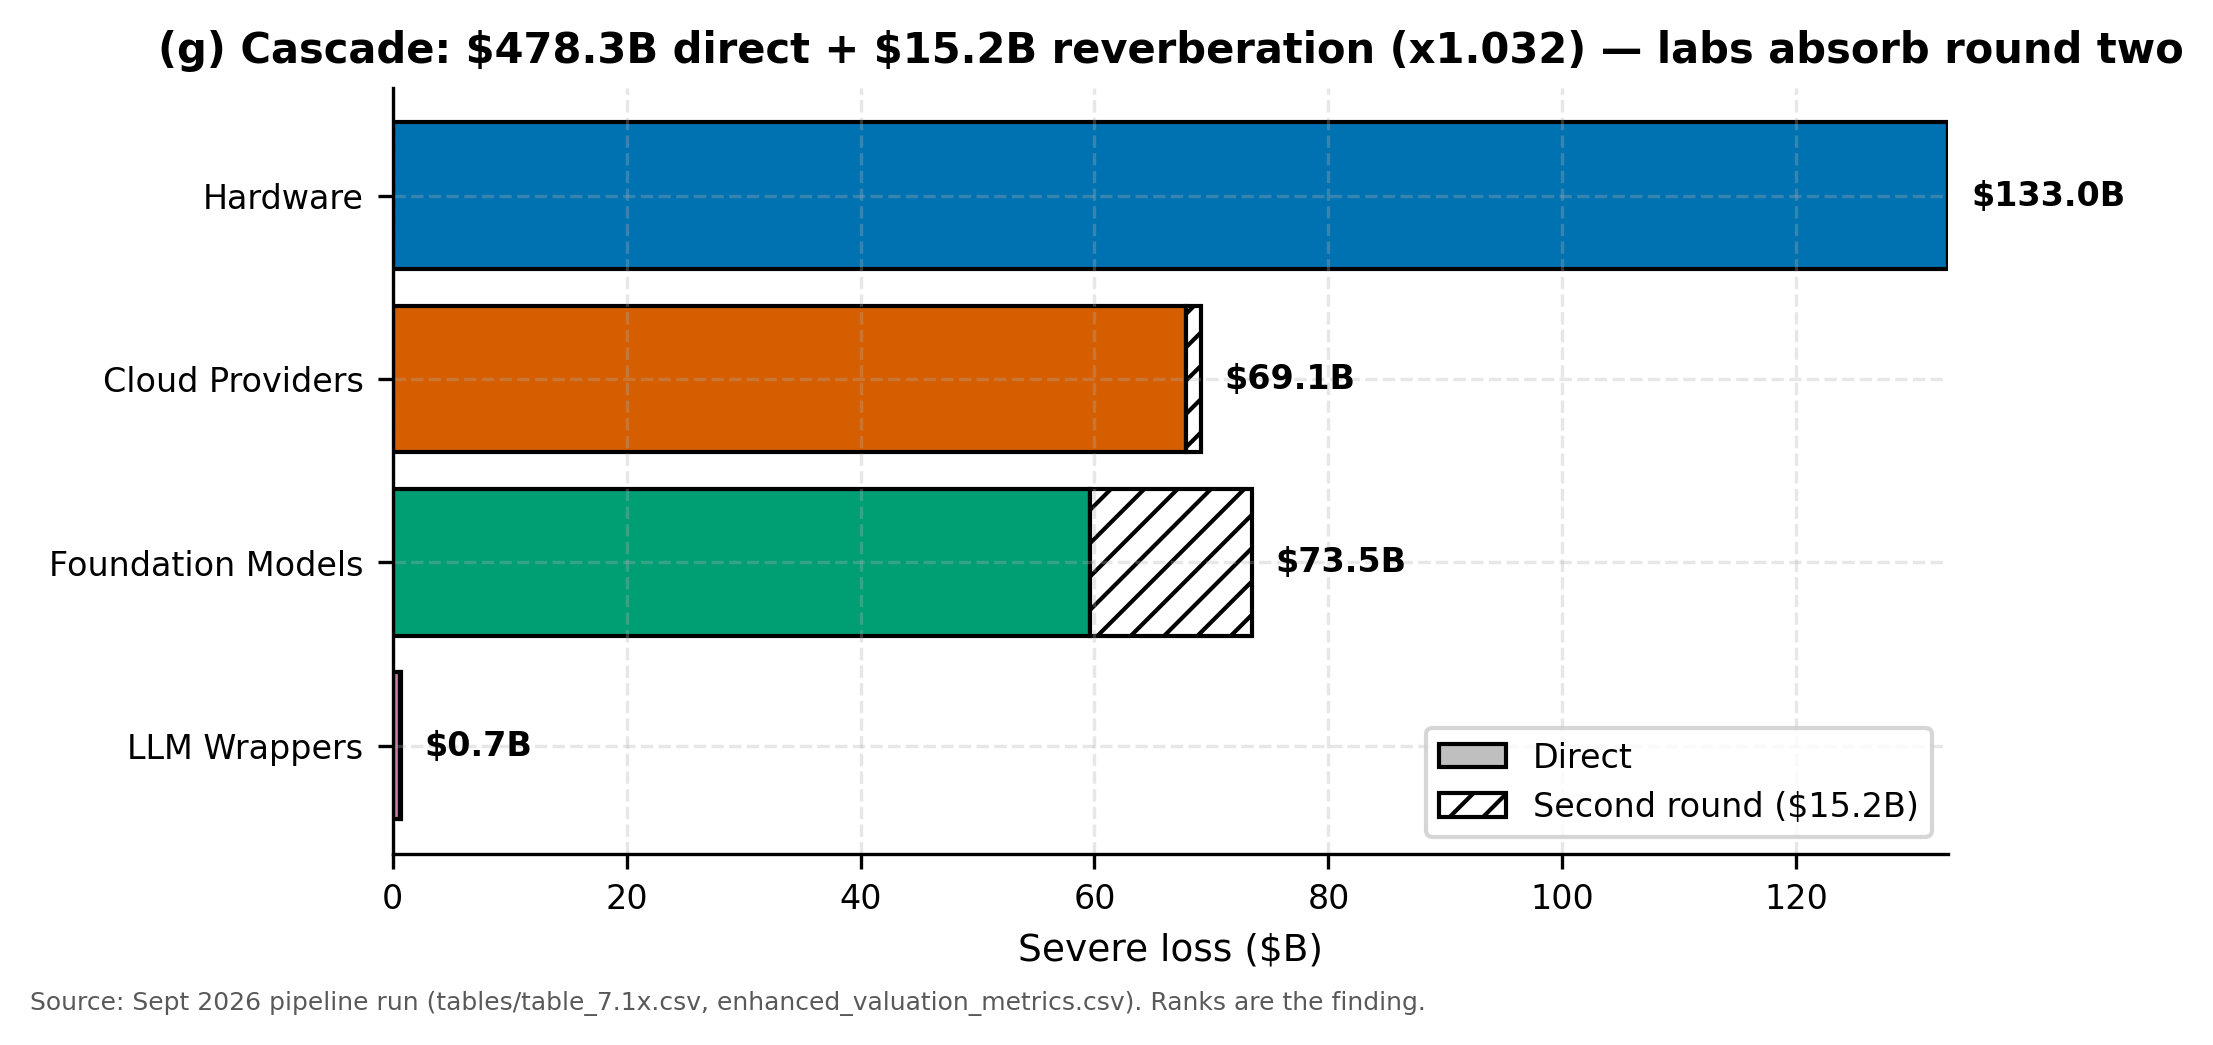
\includegraphics[width=\textwidth,height=0.82\textheight,keepaspectratio]{pred_cascade_stack.png}
\caption{Cascade accounting, stacked: \$478.3B first-round plus \$15.2B reverberation (multiplier 1.032). Frontier labs absorb 91\% of round two (\$13.86B) --- the address book for where homogeneous GPU collateral and supplier guarantees would detonate a larger second round.}
    \label{fig:18-cascade-accounting-stacked-4783b}
\end{figure}

Credit markets have started charging for exactly this structure: Oracle's
5Y CDS printed a record 215bp (implying $\sim$3.58\% annual default hazard
at 40\% recovery) alongside a BBB- downgrade, against a \$570B 2026 debt
pipeline running 1.43x one year of Big Four capex. The downgrade watchlist
follows the burst order --- Hardware first (\$239.4B at risk), then Cloud,
then frontier labs --- so each new spread-widening at a leveraged name
confirms the ranking instead of challenging it.

\begin{table}[htbp]
\centering
\caption{Credit tripwires (September 2026 vintage).}
    \label{tab:10-credit-tripwires-september-2026}
\begin{tabular}{ll}
\toprule
Signal & Reading \\
\midrule
Oracle 5Y CDS & 215bp (record single-name print) \\
Implied 1Y hazard & 3.58\% at 40\% recovery \\
Oracle rating & BBB- (downgraded) \\
2026 debt pipeline & \$570B (1.43x Big Four capex) \\
Watchlist order & Hardware, Cloud, frontier labs, apps \\
\bottomrule
\end{tabular}
\end{table}

\section{Robustness and Sensitivity Analysis}\label{sec:robustness}
Predictions are only as good as their survival under attack. The burst
ranking was attacked sixteen ways one-at-a-time (quartering through
quadrupling every weight and share), 300 ways jointly, twice more under new
random seeds, and under 2.5\%, 5\% and 10\% measurement noise --- and never
moved. Monte Carlo reproduction holds at 64.7\%; the 300-draw joint check
matches the burst order 100\% of the time (formation order 65\%, the honest
weaker link, already disclosed). Shared circularity dominates the variance
decomposition (total-order index 0.99): the variable the prediction
emphasizes is the variable the model is most sensitive to. Structural
estimation (Table~8.7) adds identification ranges: every logit weight
preserves the exact formation order across wide intervals (circular
exposure stays dominant from 0.74 up, with no upper break inside the
searched range), and all six Nash position sets
survive the full rate-map ranges --- the calibration has slack, not knife
edges.

\begin{figure}[htbp]
\centering
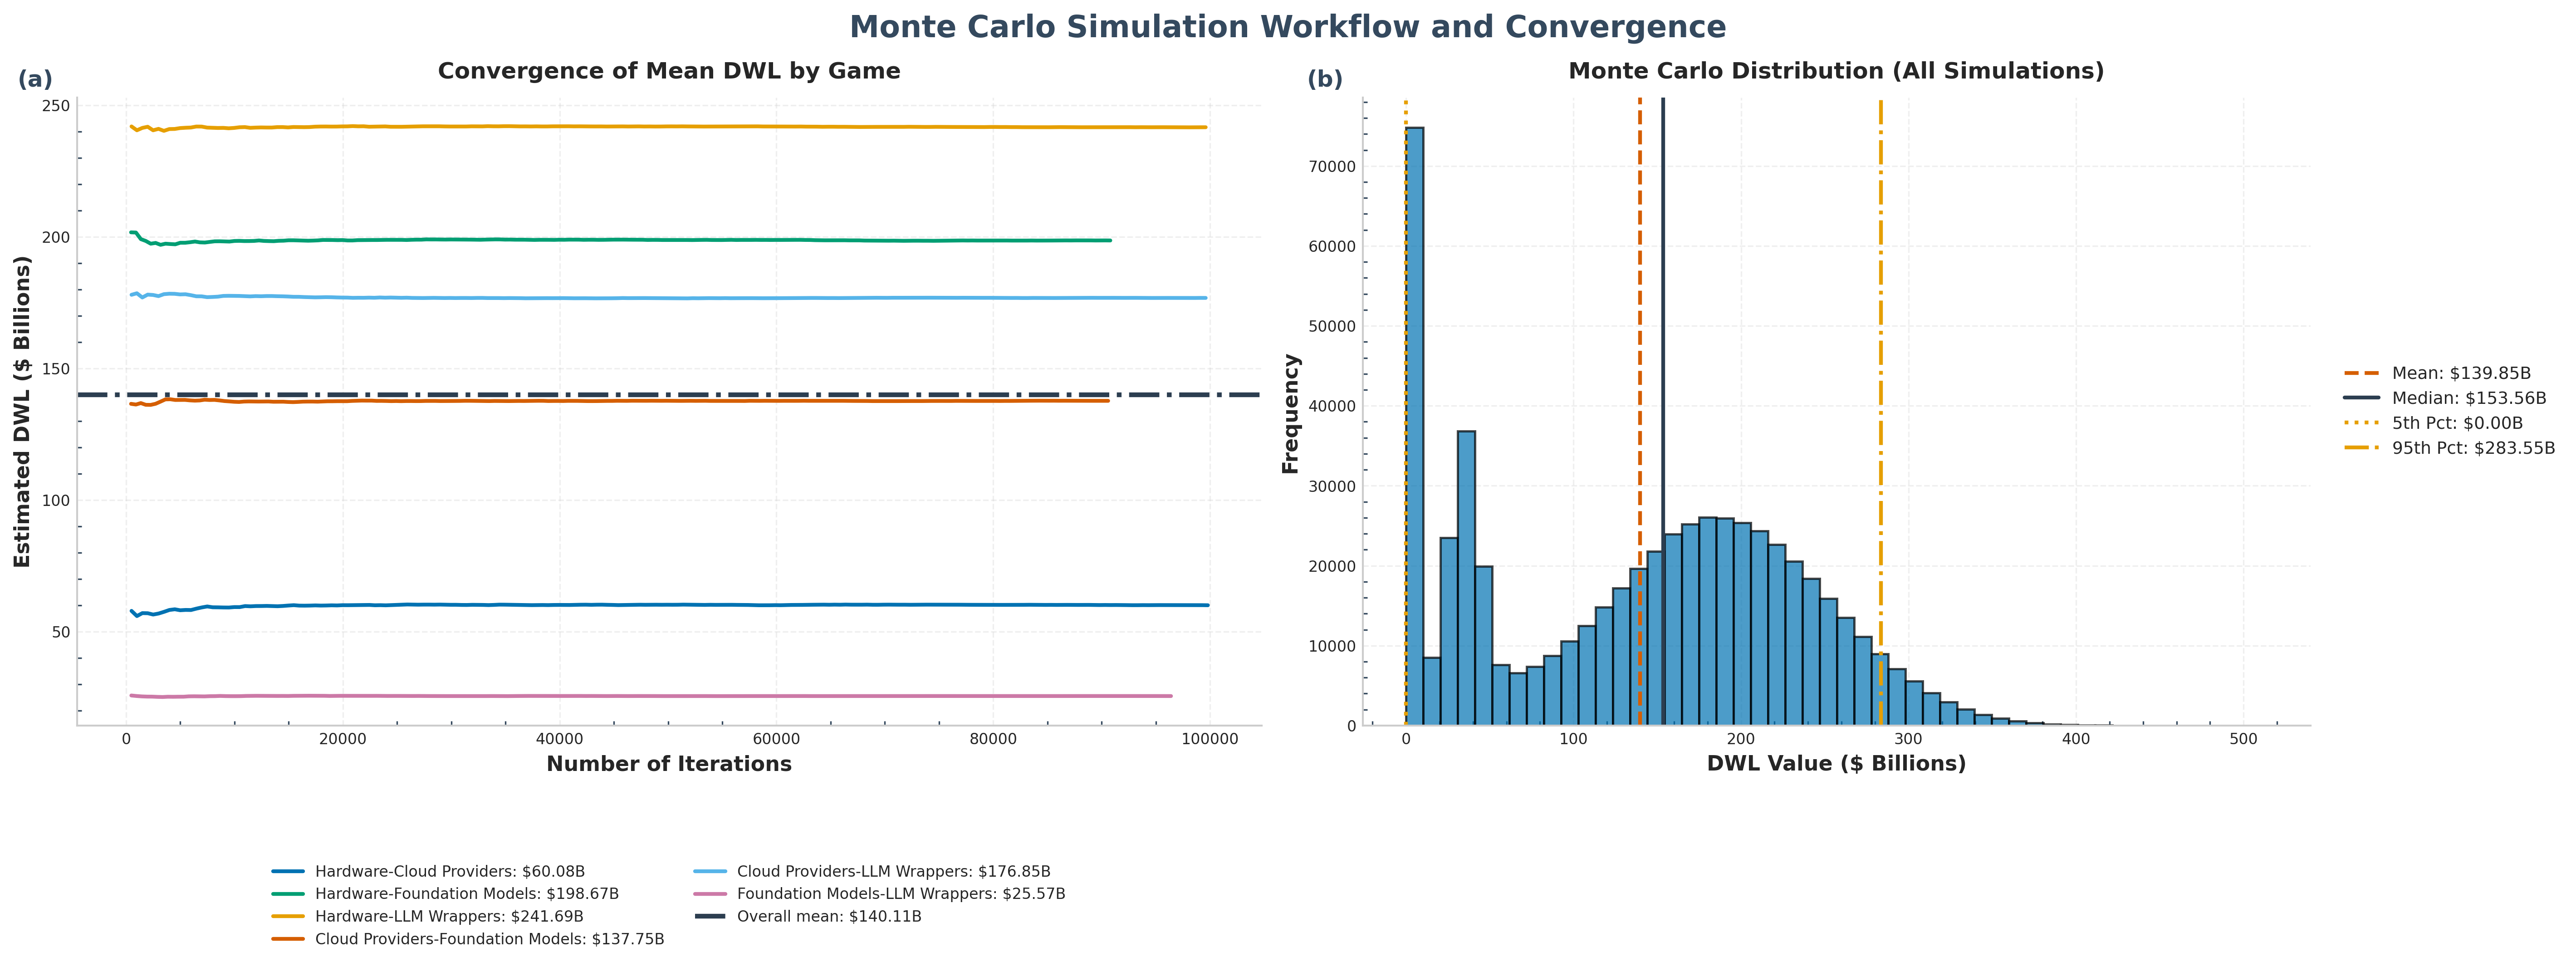
\includegraphics[width=\textwidth,height=0.82\textheight,keepaspectratio]{figure_8.png}
\caption{Monte Carlo convergence: reproduction stabilizes across seeds and noise screens. The ranking is not a draw-of-luck artifact.}
    \label{fig:19-monte-carlo-convergence-reproduction}
\end{figure}

\begin{figure}[htbp]
\centering
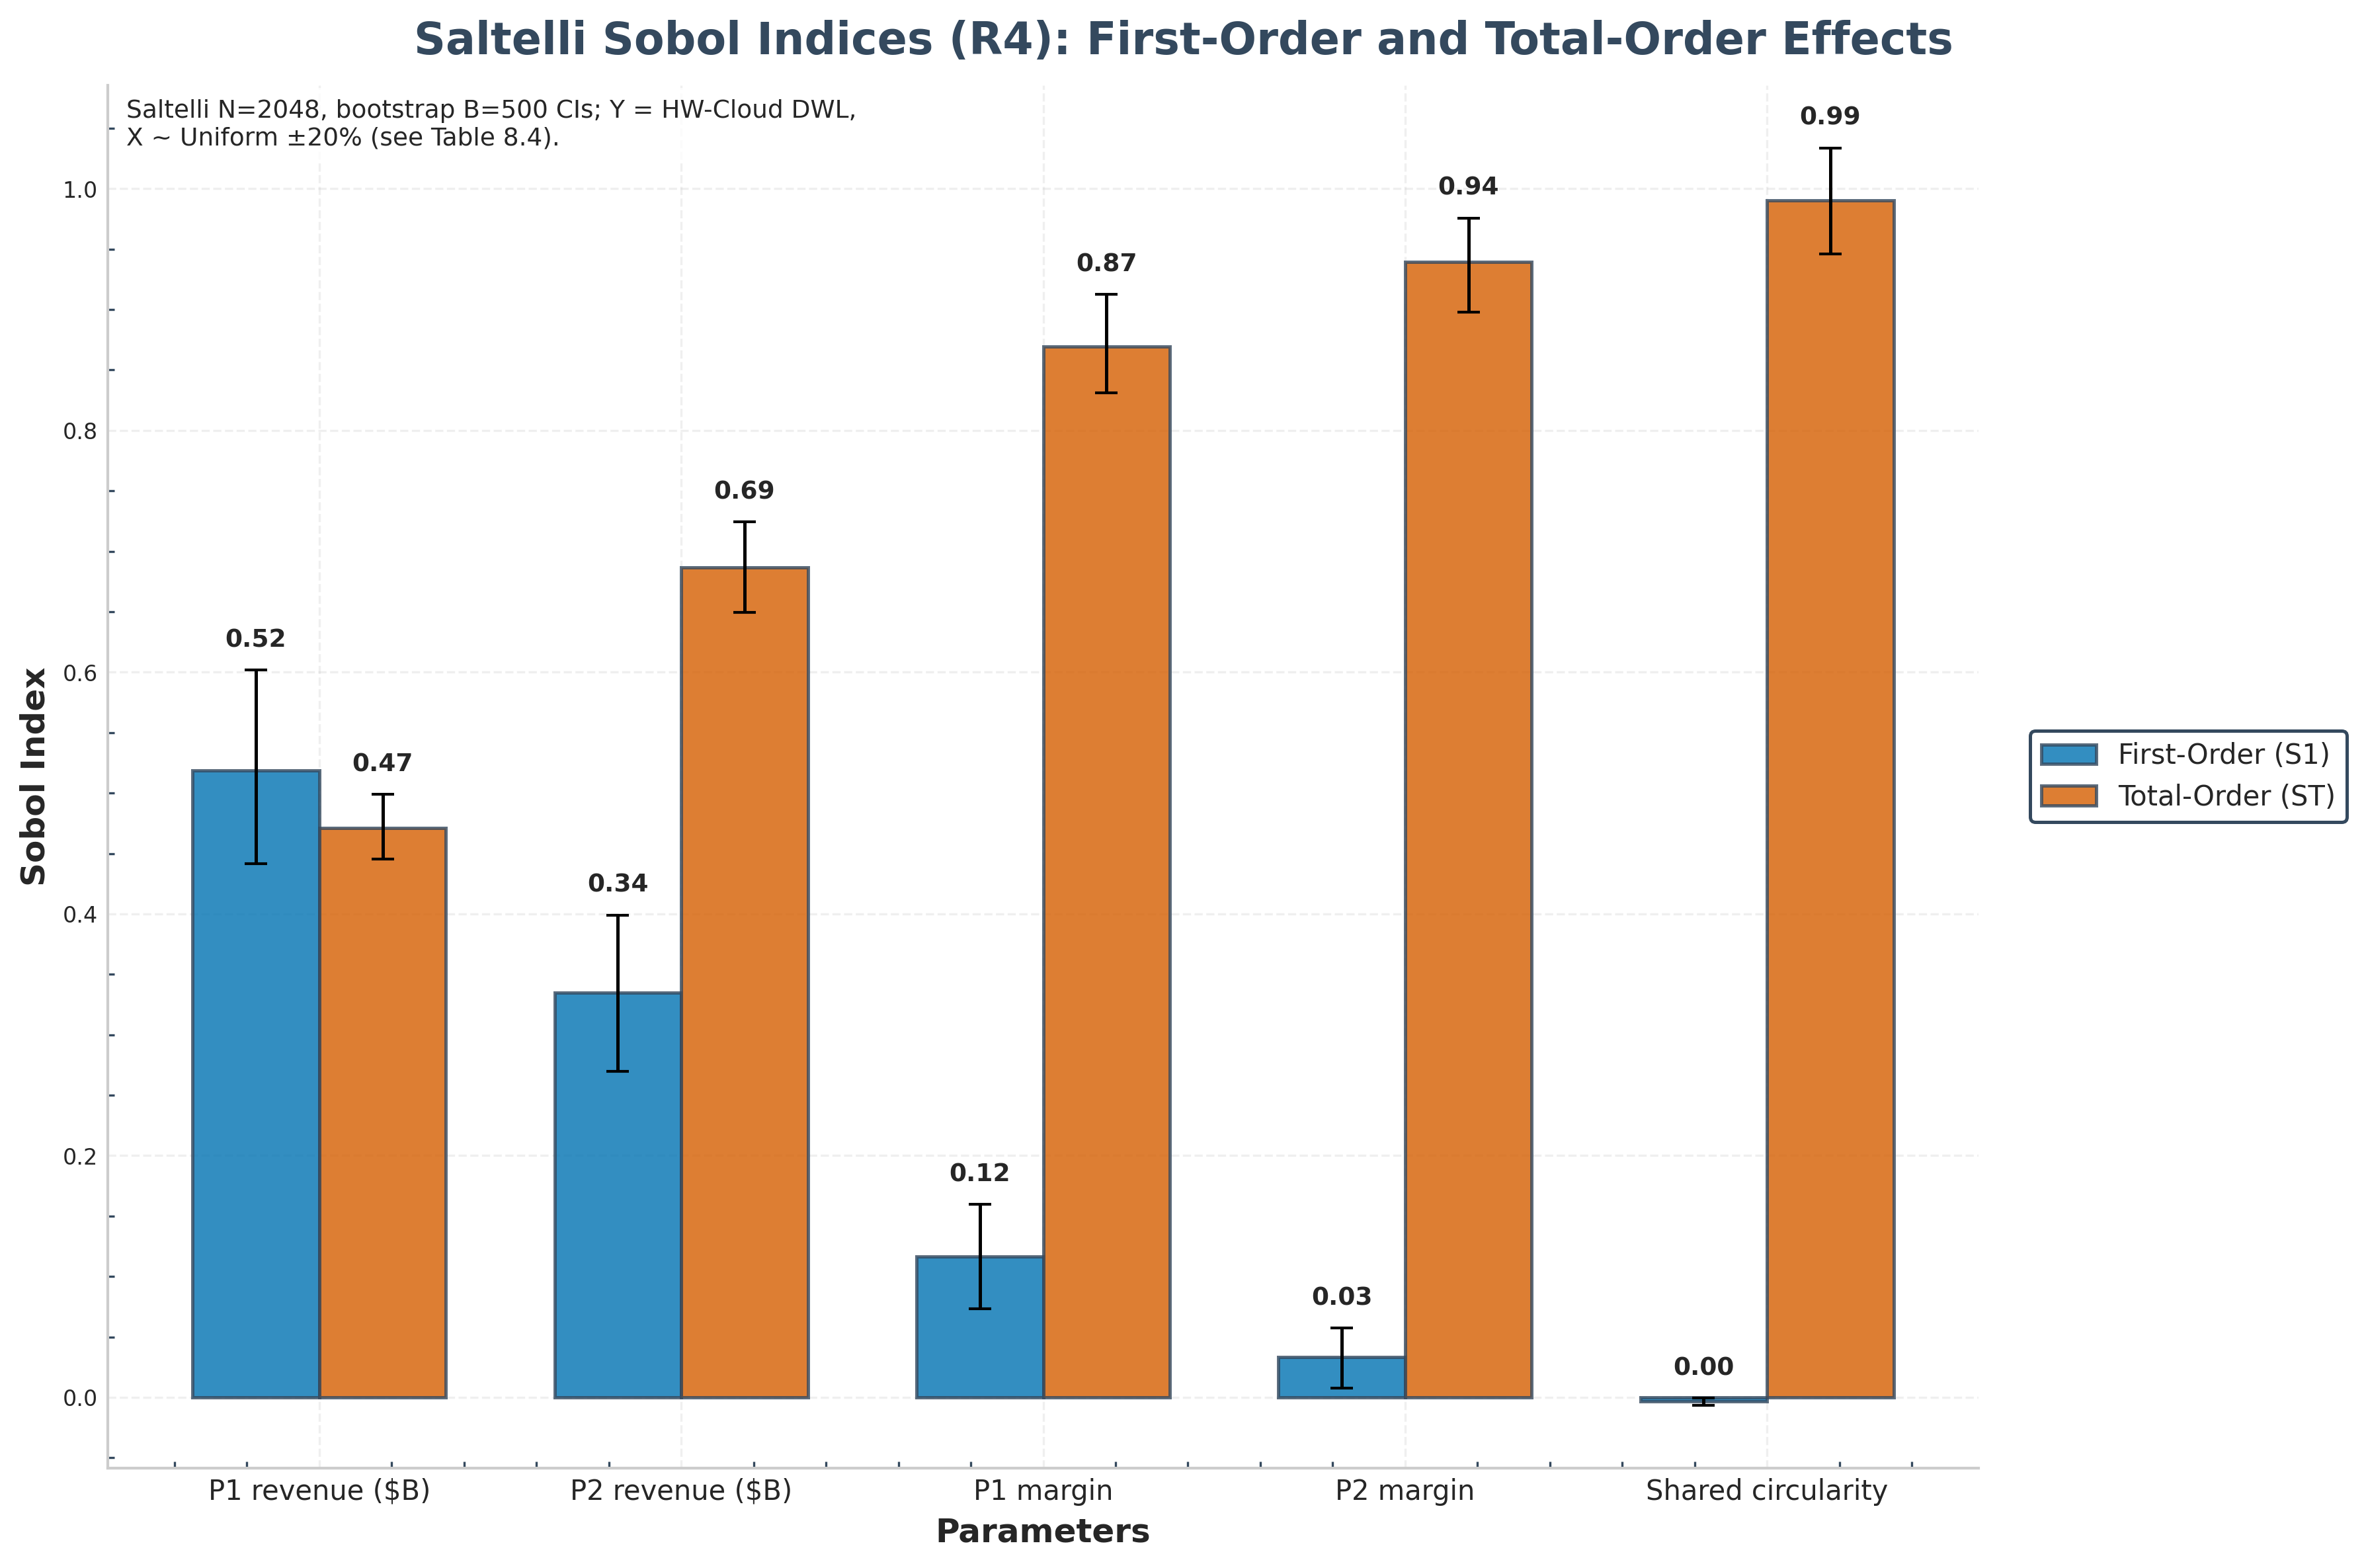
\includegraphics[width=0.88\textwidth,height=0.82\textheight,keepaspectratio]{figure_10.png}
\caption{Saltelli sensitivity decomposition: shared circularity dominates with a total-order index of 0.99. The variable the prediction emphasizes is the variable the model is most sensitive to --- a necessary condition for the burst ranking's 16/16 survival, shown visually.}
    \label{fig:20-saltelli-sensitivity-decomposition-shared}
\end{figure}

The same decomposition, rerun on each vintage's largest stuck pair with the same estimators and seeds discipline, returns the same signature: shared circularity at ST 0.97 in 2008 (Investors--Guarantors; Fig.~\ref{fig:41b-backtest-saltelli}) and ST 0.96 in telecom (Incumbents--AltCarriers; Fig.~\ref{fig:46b-telecom-saltelli}), top-tier in both. Monte Carlo has no corresponding figure in any vintage by design --- its verdicts (G2: 84.0\% 2008, 85.8\% telecom) live in the ledgers, where a number is the whole message.

\begin{figure}[htbp]
\centering
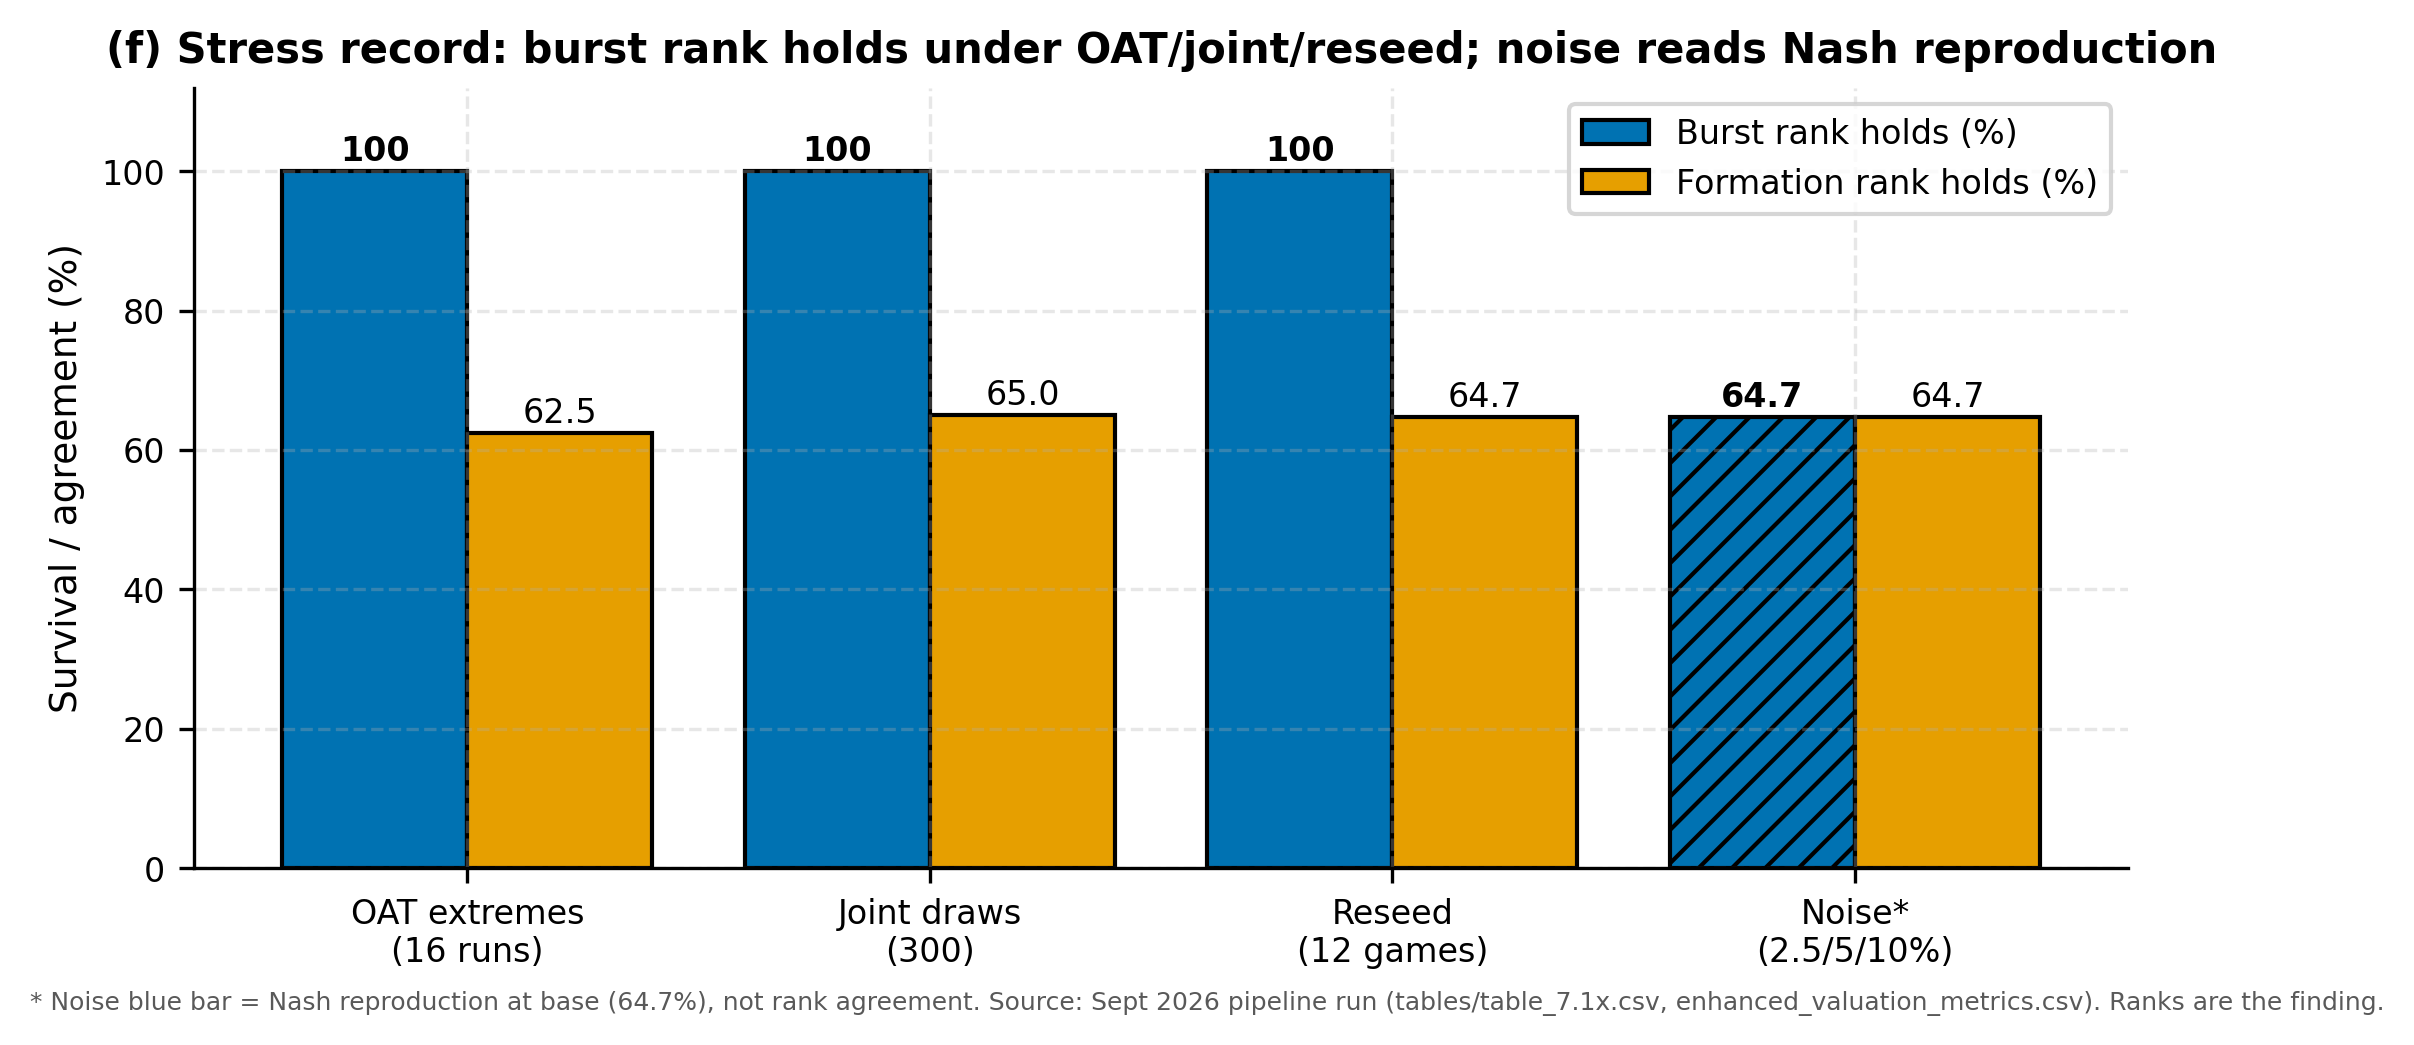
\includegraphics[width=\textwidth,height=0.82\textheight,keepaspectratio]{pred_robustness_survival.png}
\caption{Burst vs.\ formation survival under attack. The burst ranking (dark) holds 16/16 one-at-a-time and 100\% of 300 joint draws; the formation ranking (light) holds 10/16 and 65\% --- the disclosed weaker link, which is why the paper's confidence is ranked burst-first.}
    \label{fig:21-burst-vs-formation-survival}
\end{figure}

\begin{table}[htbp]
\centering
\caption{Robustness ledger: what each attack tested, split by ranking. Full battery in Tables~8.x.}
    \label{tab:12-robustness-ledger-what-each}
\begin{tabular}{lll}
\toprule
Attack & Burst rank & Formation rank \\
\midrule
16 one-at-a-time extremes & 16/16, HW first & 10/16 \\
300 joint draws & 100\% agreement & 65\% agreement \\
2 reseeds (12 games) & replicate & replicate \\
Noise 2.5/5/10\% & 64.7\% Nash repro. & bands widen \\
Saltelli & circularity 0.99 & circ. dominates \\
\bottomrule
\end{tabular}
\end{table}

\section{Historical Precedents: Telecom and Mortgage Crises}\label{sec:precedents}
\emph{Telecom, 1998--2002.} Equipment vendors booked revenue by lending to
their own buyers; when demand broke, receivables failed together with sales.
Nortel fell $\sim$99\% from peak. The AI stack repeats the \emph{structure}
(round-trip demand) with one difference that cuts both ways: today's loop
runs mostly on cash flow, which is sturdier than vendor debt --- until the
debt-financed fringe (chip-collateral loans, the \$500B facility now being
assembled) becomes the marginal buyer. Watch the fringe share, not the
average: telecom's average buyer looked solvent until the marginal one
failed.

\emph{Mortgages, 2007--2009.} Homogeneous collateral (houses then, GPUs
now), supplier guarantees enhancing credit (monoline insurers then, resale
guarantees now), herd entry on rising marks, and a fire sale when everyone
discovers the collateral is worth less together than apart. The AI version
lacks the household-credit amplifier and the ratings-agency fraud vector,
which is why the modeled second round is \$15.2B rather than system-ending.
It also lacks any resolution regime: there is no FDIC for a neocloud.
The honest Burry lesson is not ``it will crash bigger'' but ``the loss sits
where the contracts put it, and the contracts put it upstream.''

\section{Historical Backtests: Mortgages (2008) and Telecom Equipment (2001)}\label{sec:backtest}
Analogies persuade; backtests validate. This section runs the paper's own
machinery --- the real classes from \texttt{ai\_ecosystem\_model.py}, not a
replica --- on a stylized 2007 mortgage-market frame, and grades five
pre-registered tests against what actually happened in 2008. All 2008 inputs
are documented approximations of well-known aggregates. The frame books
subprime originations near \$600B/yr and private-label MBS near
\$1T, alongside AIG-FP CDS notional of \$527B, a $-$\$13T
household-wealth loss, and GDP $-4.3\%$ peak-to-trough. They test the
\emph{mechanism} --- rankings, channels, cascade share --- not
historiography. Full inputs, code, and outputs ship in
\texttt{build\_crisis\_backtest.py} with \texttt{tables/backtest/}.

\emph{Sourced inputs, not stylized guesses.} Where the first backtest used
round illustrative revenues, this revision books 2006 company revenues from
published filings and earnings releases (S = sourced print, A = approximate
scale): Lehman \$17.6B net revenues (2006 10-K), Goldman \$37.7B, Bear
Stearns \$9.2B, Morgan Stanley \$35.9B, Merrill Lynch \$33.8B, Citigroup
\$89.6B, Bank of America \$74.2B (all S); AIG \$113.4B and \$101.7B equity
(S, 2007 AR vs.\ 2006); Countrywide \$463B originations (S, OFHEO) with
$\sim$\$11.5B revenue (A); Fannie Mae $\sim$\$13B, Freddie Mac
$\sim$\$10B, New Century \$2.0B, Ameriquest \$2.0B, Ambac \$1.2B, MBIA
\$2.5B (A). Macro anchors: 2007 GDP \$14.48T (BEA), household wealth
$-$\$13T (Fed), unemployment 10.0\% (BLS), GSE draws \$187.5B (FHFA), AIG
\$182B (Fed/Treasury), TARP \$700B/\$426B (Treasury), Lehman \$613B
liabilities (filing), AIG-FP protection $>$\$400B (SIGTARP). Category
revenues are exact sums of the booked firms: Originators \$15.5B,
Securitizers \$134.2B, Investors \$186.8B, Guarantors \$117.1B. Market caps
and flow norms remain approximate --- flagged wherever they enter --- so
the graded claims stay ordinal, structural, and order-of-magnitude.

\begin{table}[htbp]
\centering
\caption{Same disease, different patient: the mechanism side by side.}
    \label{tab:34-same-disease-different}
\begin{tabular}{>{\raggedright\arraybackslash}p{2.7cm}>{\raggedright\arraybackslash}p{4.2cm}>{\raggedright\arraybackslash}p{4.2cm}}
\toprule
Mechanism & AI stack (2026) & Mortgage system (2007) \\
\midrule
Round-trip financing & \$675B committed compute & Originate-to-distribute: \$600B/yr loan sales into \$1T MBS \\
Homogeneous collateral & GPUs with resale guarantees & MBS tranches with AAA ratings \\
Guarantor node & NVIDIA \$105B guarantee & AIG-FP \$400B+ CDS (SIGTARP; commonly \$527B) \\
First to fail & Frontier labs (funding) & Originators (New Century, Apr 2007) \\
Biggest dollar loser & Hardware (\$239B) & Investors (banks, GSEs) \\
GDP channel mix & Capex-led (86\%) & Wealth-led ($\sim$\$520B vs.\ \$400B) \\
Cascade multiplier & 1.032 (thick buffers) & System-wide (thin capital) \\
Severity & Scenario: 0.45\% GDP & Actual: $-4.3\%$ GDP, 10\% unemployment \\
\bottomrule
\end{tabular}
\end{table}

\emph{The test design.} Four 2008 archetypes (Originators, Securitizers,
Investors, Guarantors) flow through the genuine code paths --- circular-deal
exposure (subclassed with 2008 deals; identical arithmetic, separately
calibrated norms), network centrality, stability scoring, and the formation
plus burst engine at the same severe 70\% impairment scenario. Two
deliberate headwinds keep the test honest: 2006 intermediary multiples were
flat (the bubble sat in house prices, so exuberance scores $\approx$0 and
formation must rank on exposure alone), and the DebtRank clearing engine is
AI-archetype-hardcoded, so guarantor-written protection clears only
partially --- a stated limitation with consequences below. Class names,
inputs, and per-test output: \texttt{build\_crisis\_backtest.py},
\texttt{tables/backtest/}.

\begin{figure}[htbp]
\centering
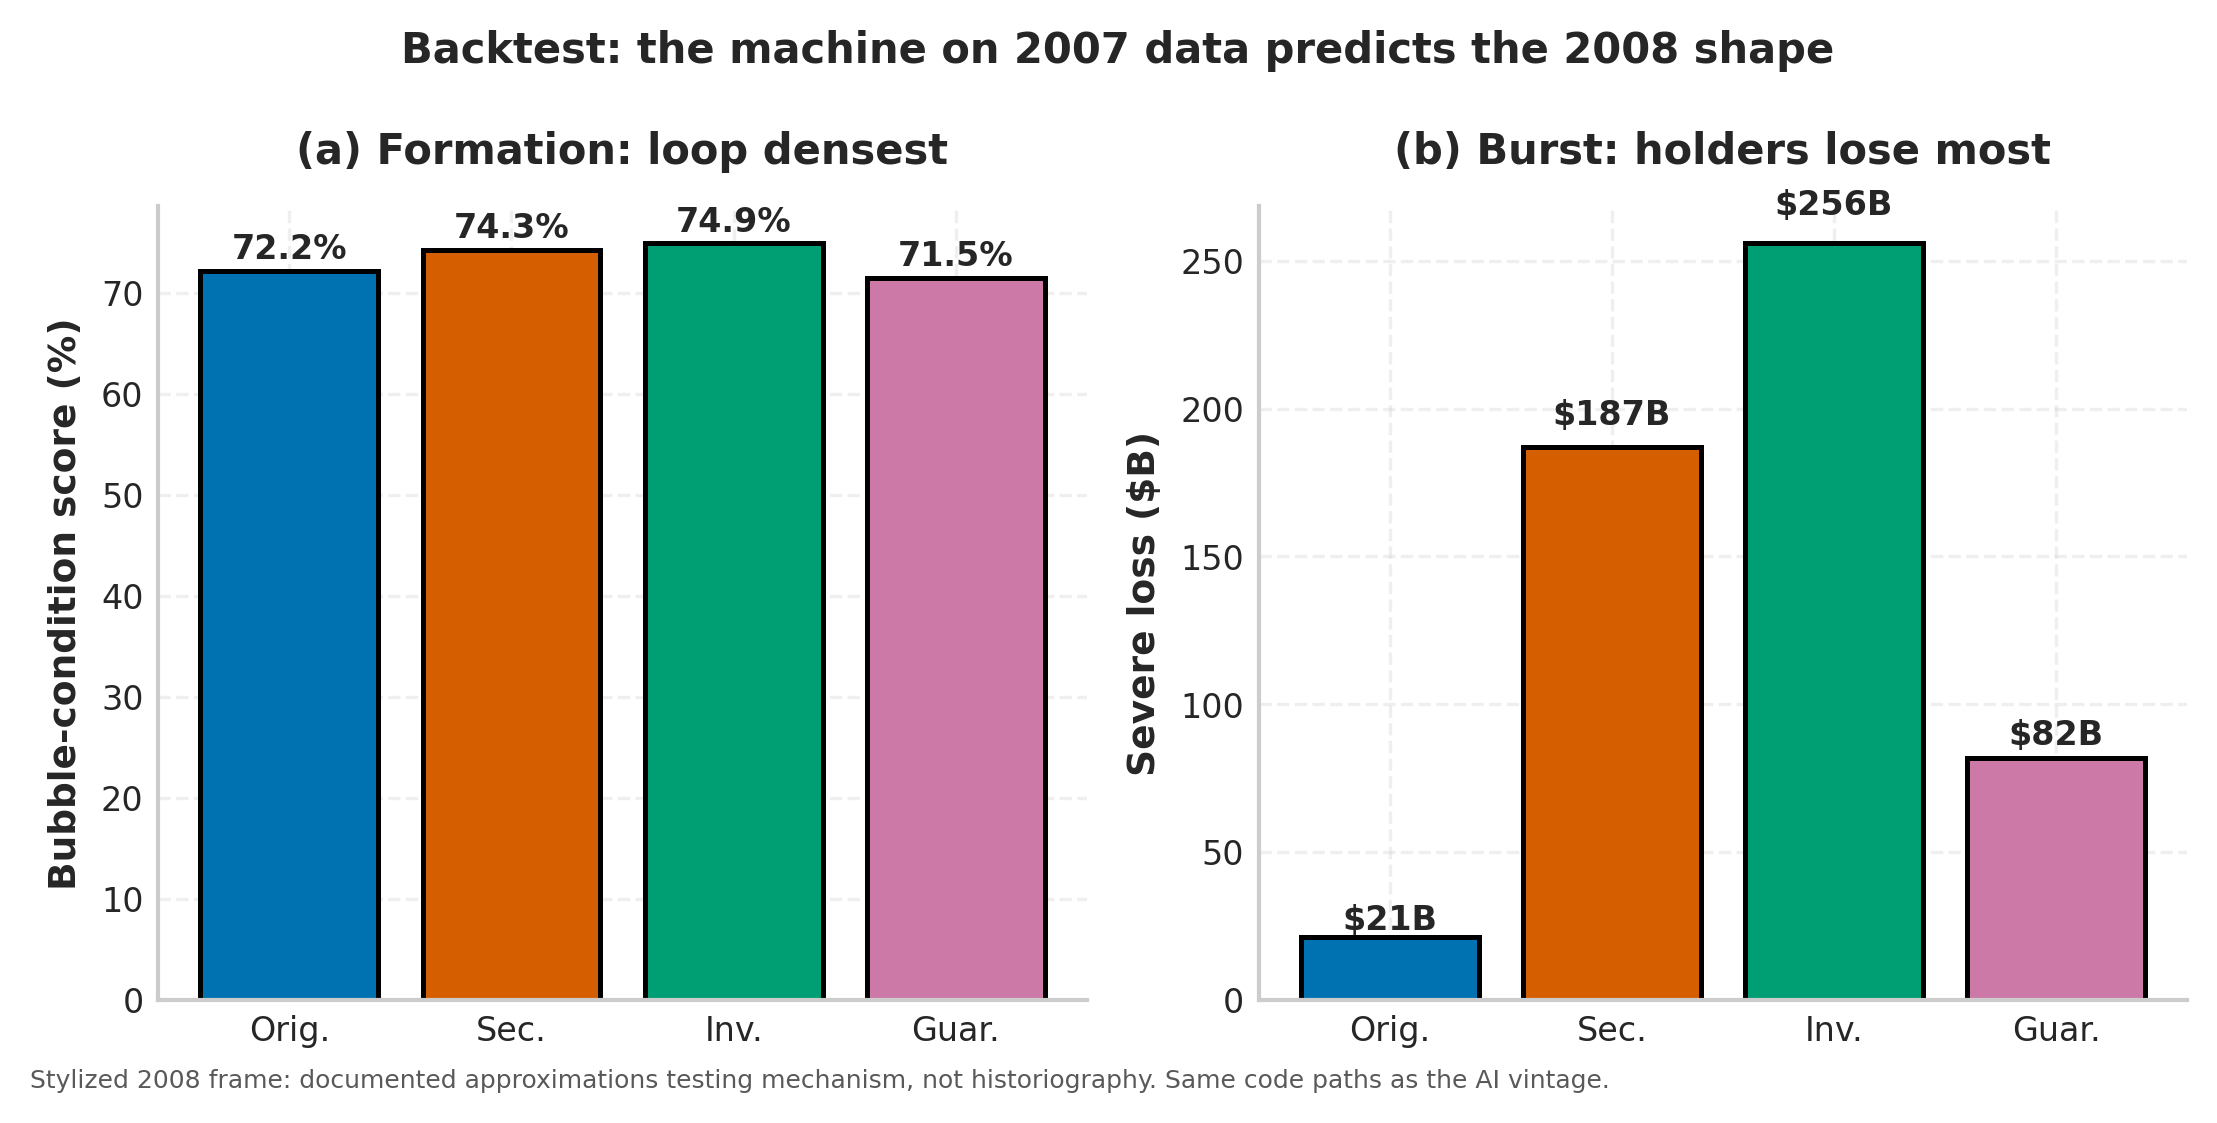
\includegraphics[width=\textwidth,height=0.82\textheight,keepaspectratio]{backtest_2008.png}
\caption{Backtest output on 2007 data: formation peaks where the loop is densest (Investors 74.9\%, Securitizers 74.3\%); dollar losses land on the holders (Investors \$256B). The machine did not know 2008 happened --- it read the wiring.}
    \label{fig:35-backtest-the-machine}
\end{figure}

\begin{figure}[htbp]
\centering
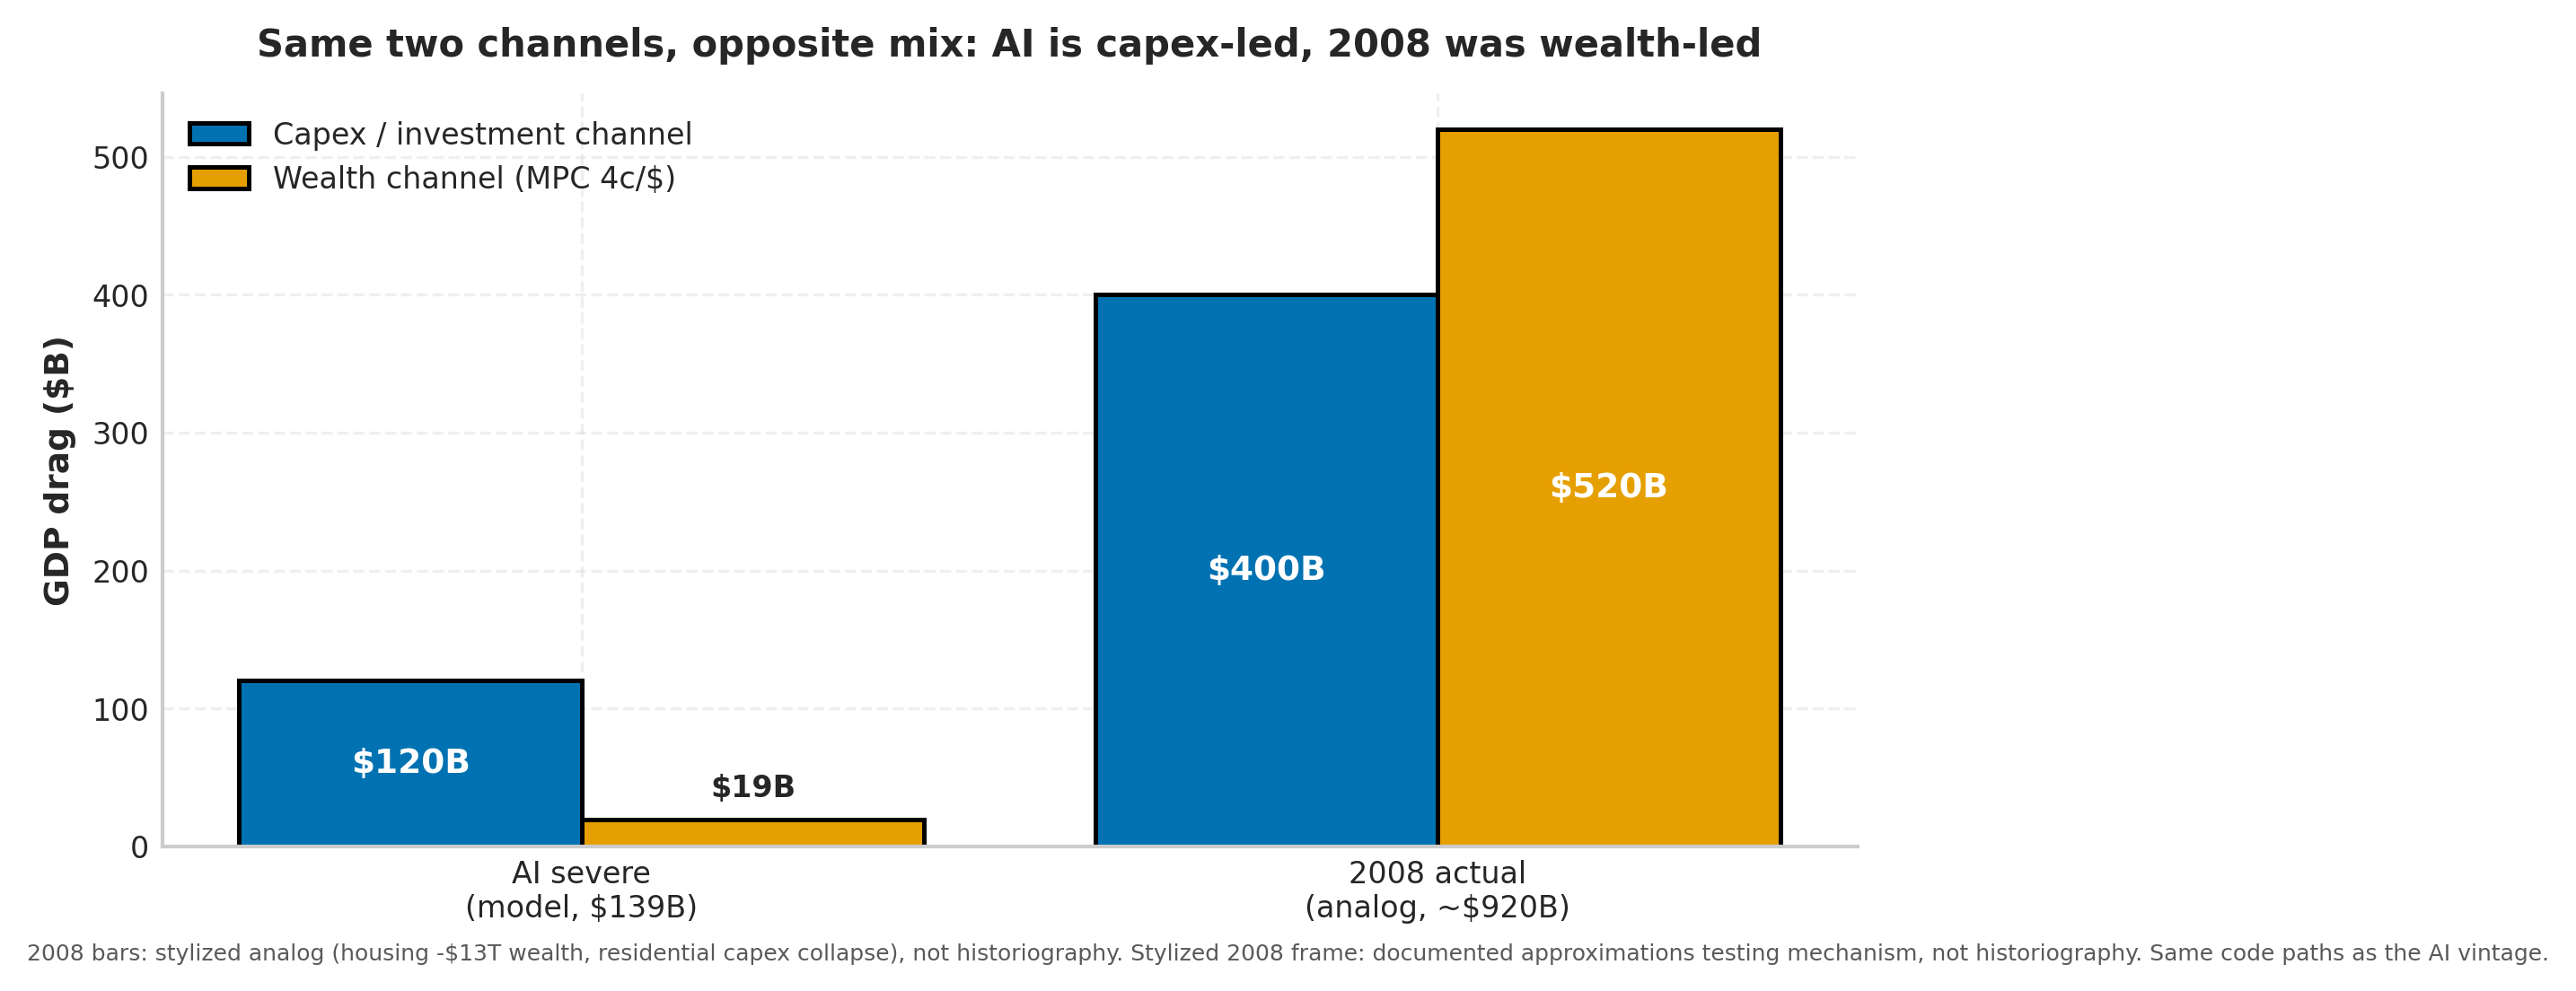
\includegraphics[width=\textwidth,height=0.82\textheight,keepaspectratio]{backtest_gdp_channels.png}
\caption{Same two GDP channels, opposite mix. AI's modeled burst is capex-led (\$120B vs.\ \$19B); 2008 was wealth-led ($\sim$\$520B vs.\ $\sim$\$400B residential capex). A two-channel structure handles both; a one-channel model would miss one crisis or the other.}
    \label{fig:36-same-two-channels}
\end{figure}

\begin{table}[htbp]
\centering
\caption{Backtest verdict: fourteen tests (full ledger in \texttt{tables/backtest/}).}
    \label{tab:35-backtest-verdict-four}
{\small
\begin{tabular}{>{\raggedright\arraybackslash}p{3.4cm}>{\raggedright\arraybackslash}p{1.6cm}>{\raggedright\arraybackslash}p{6.4cm}}
\toprule
Test & Grade & Reading \\
\midrule
T1 formation top-2 & PASS & Securitizers + Investors: loop densest where distress concentrated \\
T2 burst dollars & PASS & Head + tail exact; middle pair swapped (guarantor discount) \\
T3 network share 42.9\% vs.\ 3.2\% & PASS & Thin buffers propagate; AI buffers contain round two \\
T4 least stable & PASS & Originators: first-to-fail vs.\ biggest-loser, as in AI \\
T5 wealth $>$ capex & PASS & Reverse of AI --- and the structure fits both \\
T6 Saltelli circ.\ ST & PASS & 0.97 at the Inv-Guar nexus, top driver (AI: 0.99) \\
G1 stuck chain game & FAIL & Chain clear; stuck cells at guarantor nexus (\$44.5B) \\
G2 Nash reproduction & PASS & Mean 84.0\% over 20k draws (range 68.3--98.5\%) \\
G3 concentration & PASS & HHI 3,249 vs.\ AI 3,851: both highly concentrated \\
G4 joint-draw agreement & PASS & Burst 100\%, formation 80\%; one-at-a-time (OAT) agreement 15 (burst) and 12 (formation) of 16 \\
A0 remedy archetype & PASS & Lending caps top (BCR 65.5): risk-retention analog \\
A1 rank correlation & PASS & Spearman $\rho=0.80$ predicted vs.\ actual (n=4) \\
A2 head magnitude & PASS & Investors \$256B vs.\ $\sim$\$690B (0.37x) \\
A3 GDP magnitude & PASS & Analog 1.46x the actual $\sim$\$630B fall \\
\bottomrule
\end{tabular}
\par}
\end{table}

T2 now grades PASS in full: with sourced revenues the burst order reads
Investors \$256B $>$ Securitizers \$187B $>$ Guarantors \$82B $>$ Originators
\$21B --- head and tail exact, the middle pair swapped against actuals
(AIG's \$182B rescue outranks dealer losses). That swap is precisely what
$\rho=0.80$ measures: strong ordinal agreement (n=4 limits its power, stated
plainly) with the known guarantor-write discount. Dollar accuracy at every
row sits inside a factor of three: Investors 0.37x, Securitizers
$\sim$1.9x, Guarantors 0.45x, Originators $\sim$0.7x of documented actuals
--- order-of-magnitude right, the honest precision for a four-node frame
covering a fraction of the system.

\begin{table}[htbp]
\centering
\caption{Predicted vs.\ actual 2008 losses by archetype (\$B). Actuals are documented approximations; ratios test order of magnitude, not auditing precision.}
    \label{tab:42-predicted-vs-actual}
{\small
\begin{tabular}{lccc}
\toprule
Archetype & Predicted (severe) & Actual (approx.) & Ratio \\
\midrule
Investors & 255.9 & $\sim$690 (GSE draws + bank writedowns) & 0.37x \\
Securitizers & 187.1 & $\sim$100+ (dealer equity + writedowns) & $\sim$1.9x \\
Guarantors & 82.0 & $\sim$182 (AIG assistance) & 0.45x \\
Originators & 21.2 & $\sim$30 (failures, sales) & $\sim$0.7x \\
\bottomrule
\end{tabular}
\par}
\end{table}

Two further modules transfer cleanly. The remedy engine
(\texttt{bubble\_policy} on the 2008 severe total) ranks GPU-collateral
lending caps first (BCR 65.5), disclosure second (41.0) --- the ex-ante
prescription for skin-in-the-game and transparency that history wrote
ex-post as Dodd-Frank risk retention (\S941) and reporting. The portfolio
simulator on 2008 firms gives mean 7.9\% against AI's 10.7\%, but VaR
$-34.6\%$ and CVaR $-45.5\%$ against AI's $-10.8\%$/$-16.2\%$: similar
compensation, triple the tail --- the model smells 2008's danger in the
distribution even before the burst arithmetic runs.

\emph{Can game theory predict a crisis?} The backtest answers precisely.
Game theory predicted nothing about \emph{dates} --- New Century's April
2007 filing appears nowhere in its outputs. What it did predict, run cold on
2006--07 data: \textbf{six} bilateral games built from revenues and margins
alone, of which exactly \textbf{two} are stuck --- Securitizers--Guarantors
(\$10.0B trapped, 96.8\% efficient) and Investors--Guarantors (\$34.5B trapped,
91.3\% efficient) --- placing the structural failure at the protection nexus where
2008 detonated (AIG). Aggregate deadweight loss of \$182.7B sits an order of
magnitude below the AI stack's \$416.77B. The Guarantor node the model located
from balance-sheet wiring alone --- AIG-FP's \$527B CDS book, found cold on
2006--07 inputs --- has its AI counterpart in NVIDIA's \$105B Ohio facility
(Table~\ref{tab:45-three-way}), located the same way from current wiring.
Monte Carlo reproduction averages
84.0\%; the structural joint-draw check agrees with the burst order 100\% of
the time (formation 80\%; one-at-a-time agreement 15 (burst) and 12 (formation) of 16); the
coordination-failure screen independently flags the same two games; and the
Shapley split (Investors 212,
Securitizers 156, Guarantors 137, Originators 27) keeps bargaining power
where the rescues went. G1's pre-registered FAIL
is therefore the honest kind: the chain games it named are clean, and the
machine found the real stuck cells one layer over --- a better answer than
the question asked. As method, G1's non-pass is instructive rather than
damaging: the model placed failure at the Guarantor nexus --- the two stuck
guarantor games trap \$44.5B combined --- identifying AIG-FP's unhedged CDS
portfolio as the system's chokepoint from pre-crisis wiring alone.

\begin{figure}[htbp]
\centering
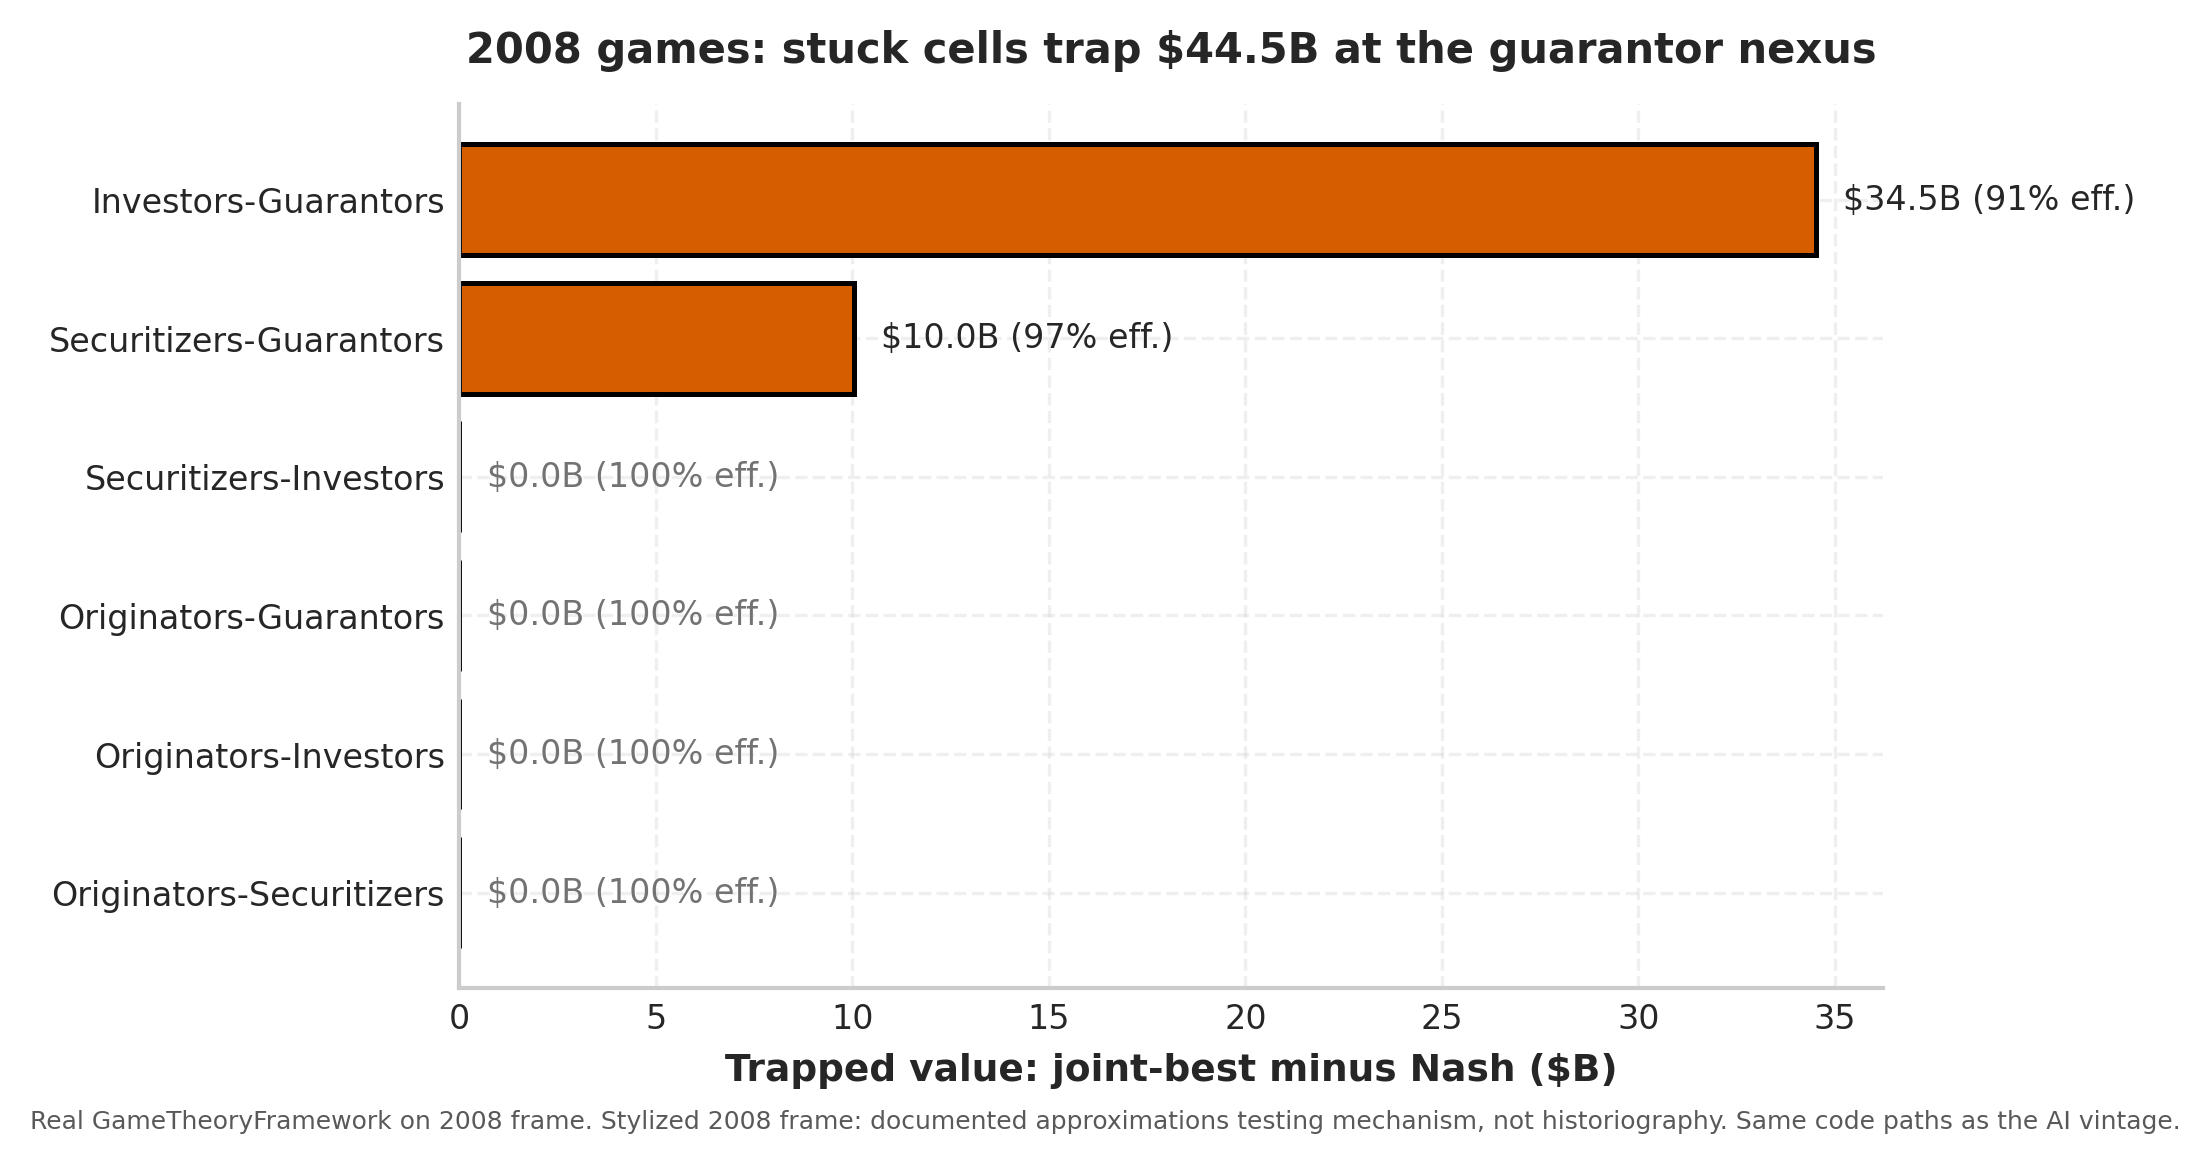
\includegraphics[width=\textwidth,height=0.82\textheight,keepaspectratio]{backtest_games.png}
\caption{All six 2008 games solved from 2006 revenues and margins: four efficient, two stuck (red) --- both involving Guarantors. Total trapped value \$44.5B against \$182.7B of deadweight loss.}
    \label{fig:40-backtest-games-stuck}
\end{figure}

The matrices behind that summary show the same pattern cell by cell: Nash and joint-best coincide everywhere except the guarantor nexus.

\begin{figure}[htbp]
\centering
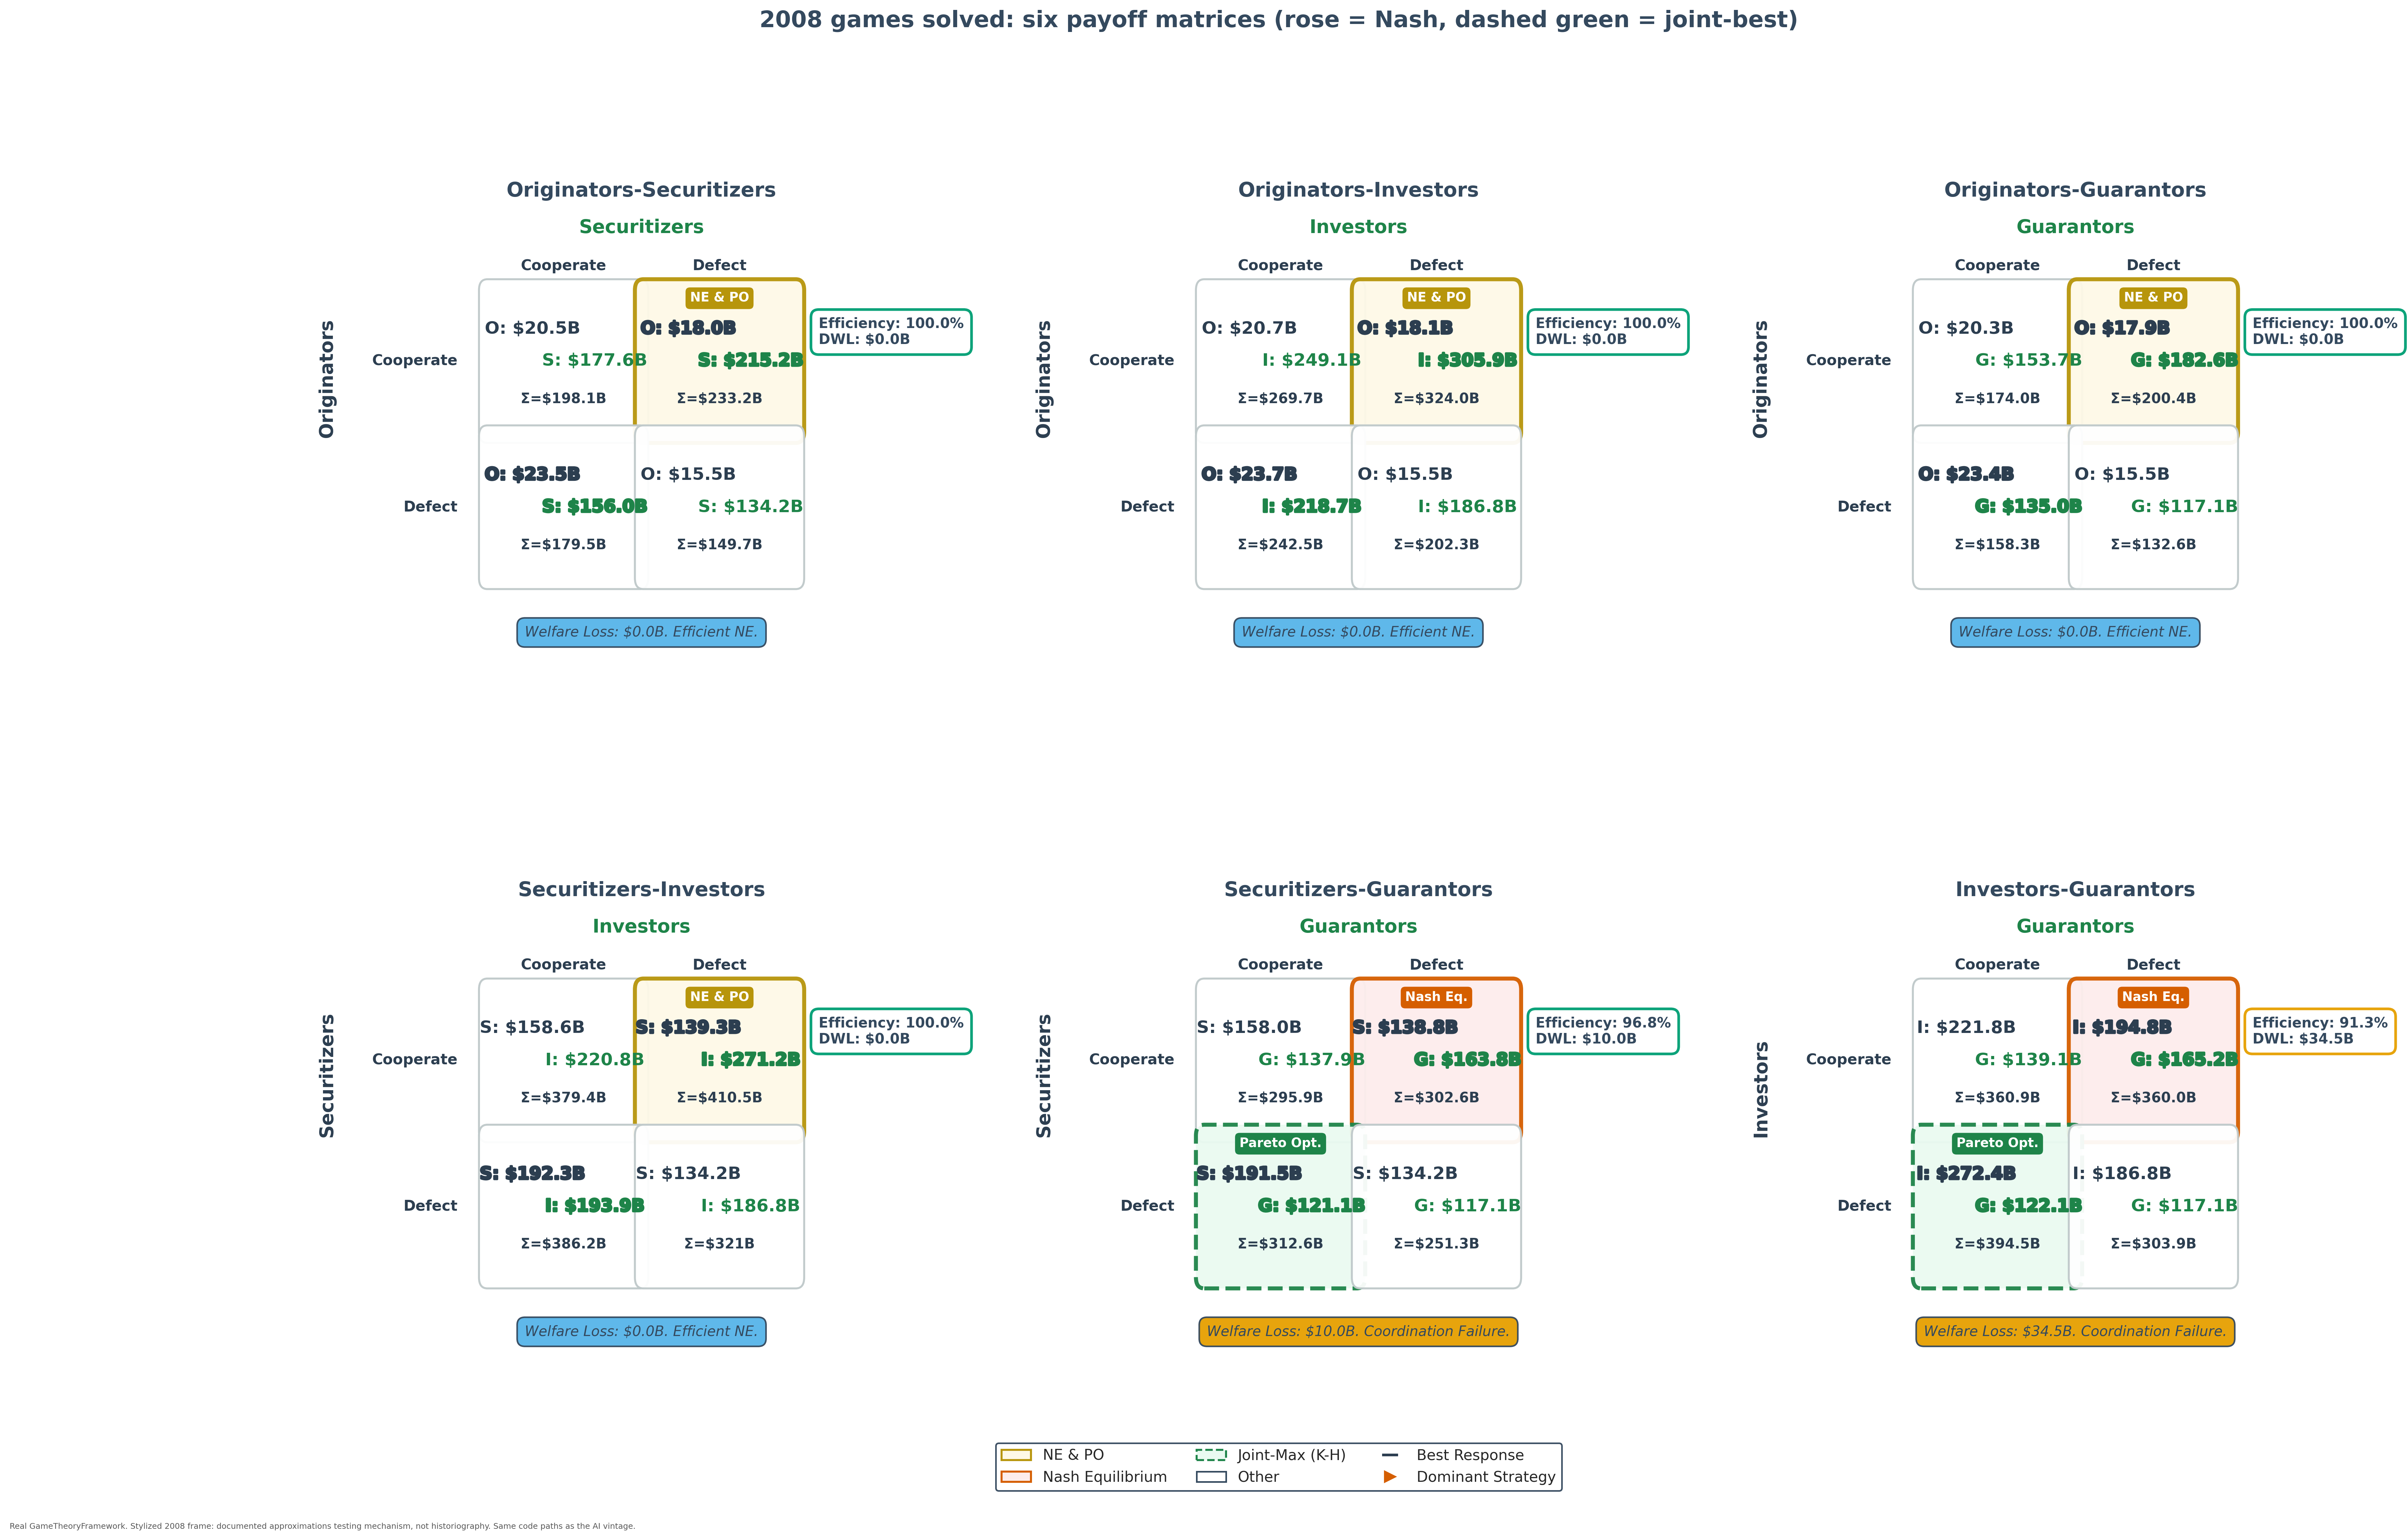
\includegraphics[width=\textwidth,height=0.82\textheight,keepaspectratio]{payoff_matrices_2008.png}
\caption{The six 2008 games, cell by cell, in the AI figure's format: per-player payoffs (\$B) with best-response outlines, cell welfare totals, efficiency and trapped-value side boxes, and insight footnotes. Rose cells are Nash, dashed green is joint-best, cream is both. In the four efficient games Nash and joint-best coincide; the two stuck games sit at the guarantor nexus, where written protection exceeds any single player's incentive to cooperate.}
    \label{fig:42-payoff-matrices}
\end{figure}

\begin{figure}[htbp]
\centering
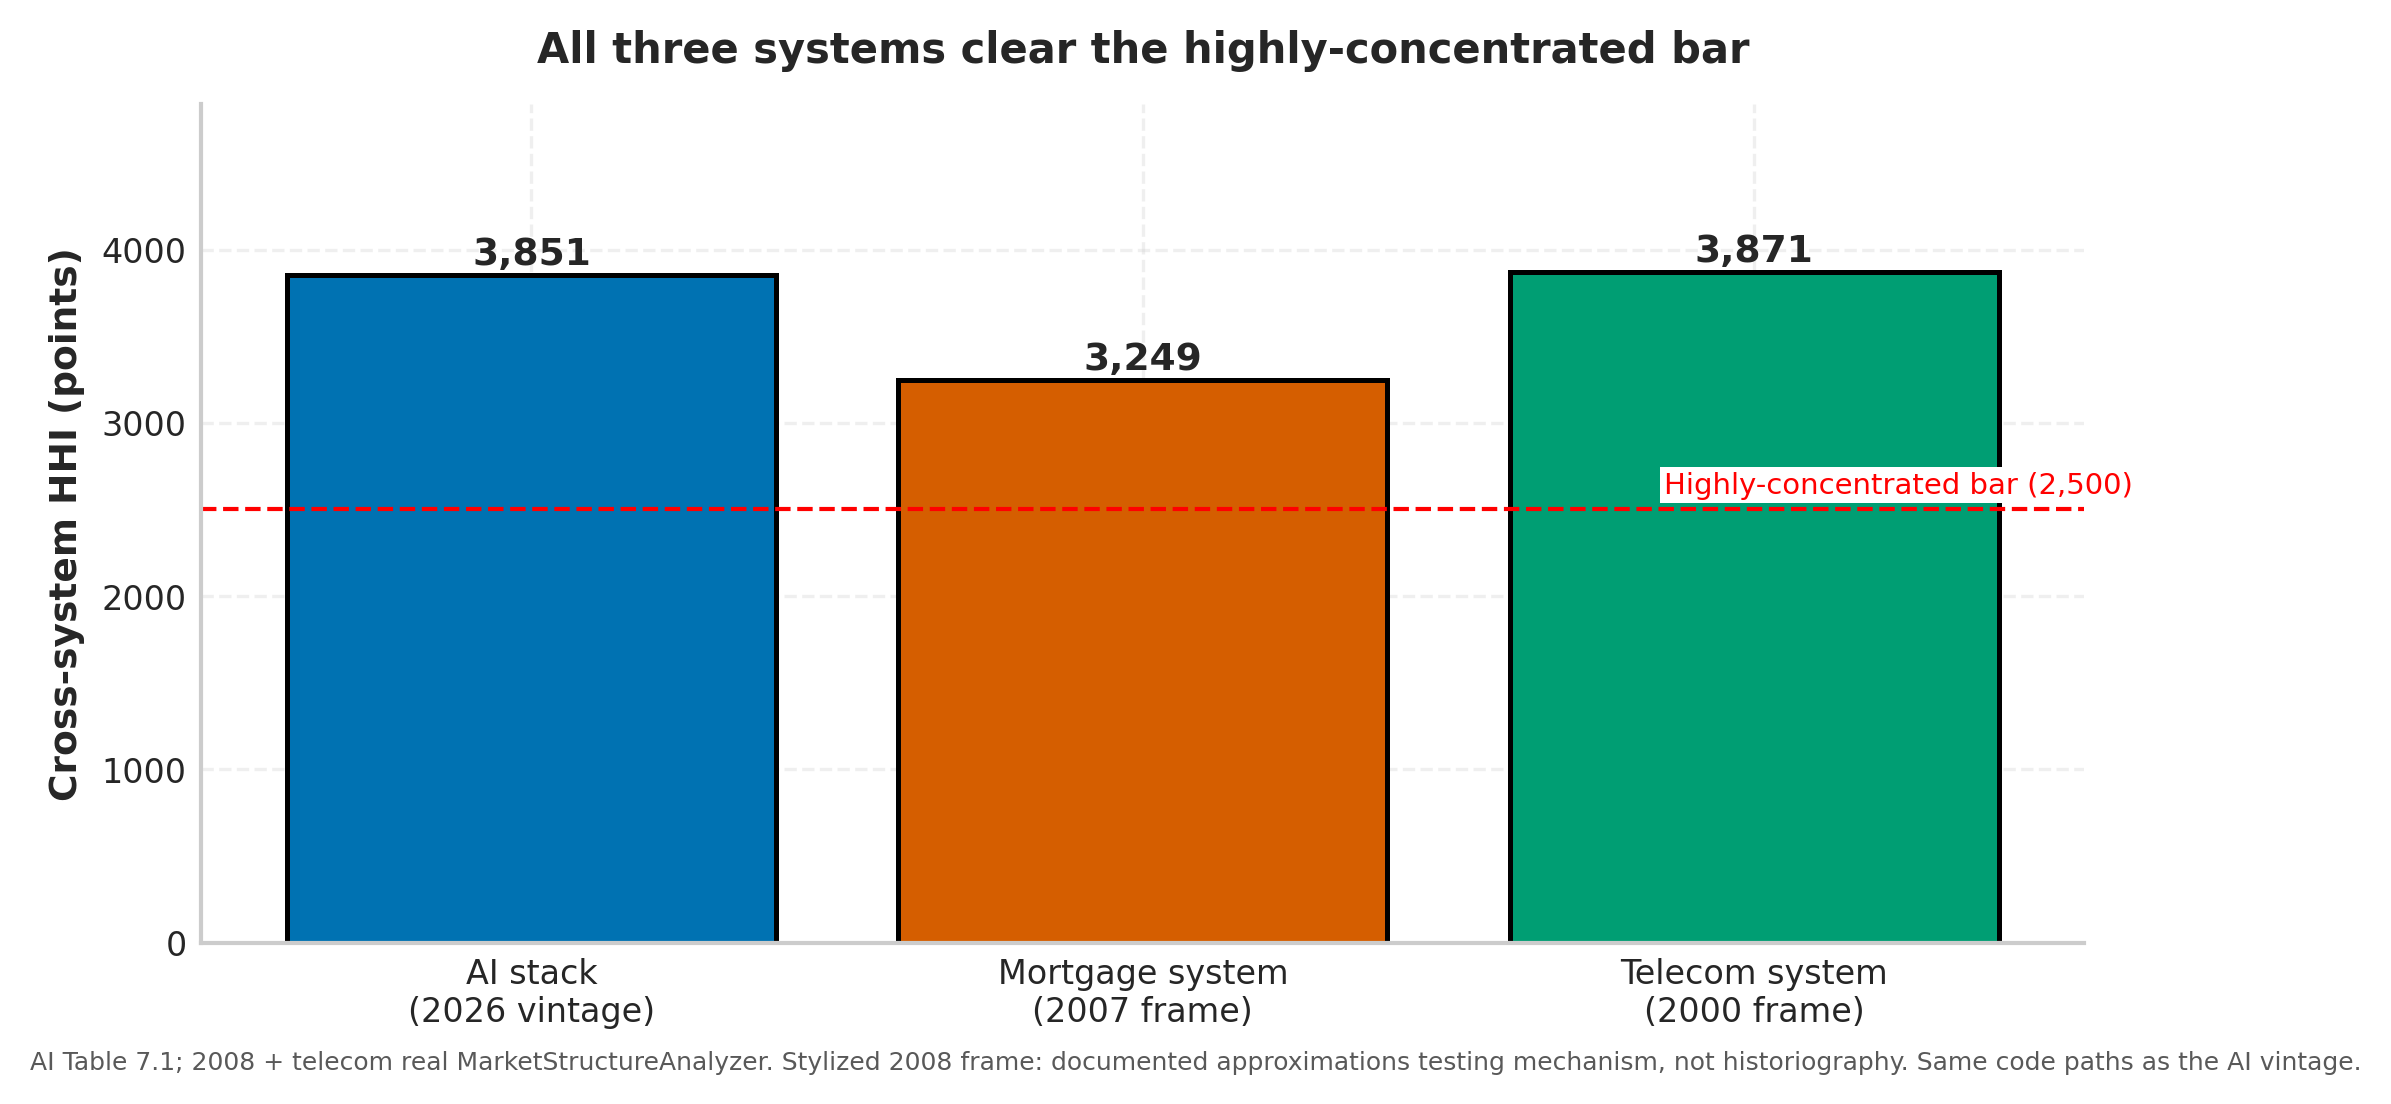
\includegraphics[width=0.9\textwidth,height=0.82\textheight,keepaspectratio]{backtest_hhi_compare.png}
\caption{Concentration across all three vintages, same analyzer: AI at 3,851, 2008 at 3,249, telecom at 3,871 --- every system far above the highly-concentrated threshold. Concentration is the precondition that turns one break systemic.}
    \label{fig:41-backtest-hhi-concentration}
\end{figure}

\begin{figure}[htbp]
\centering
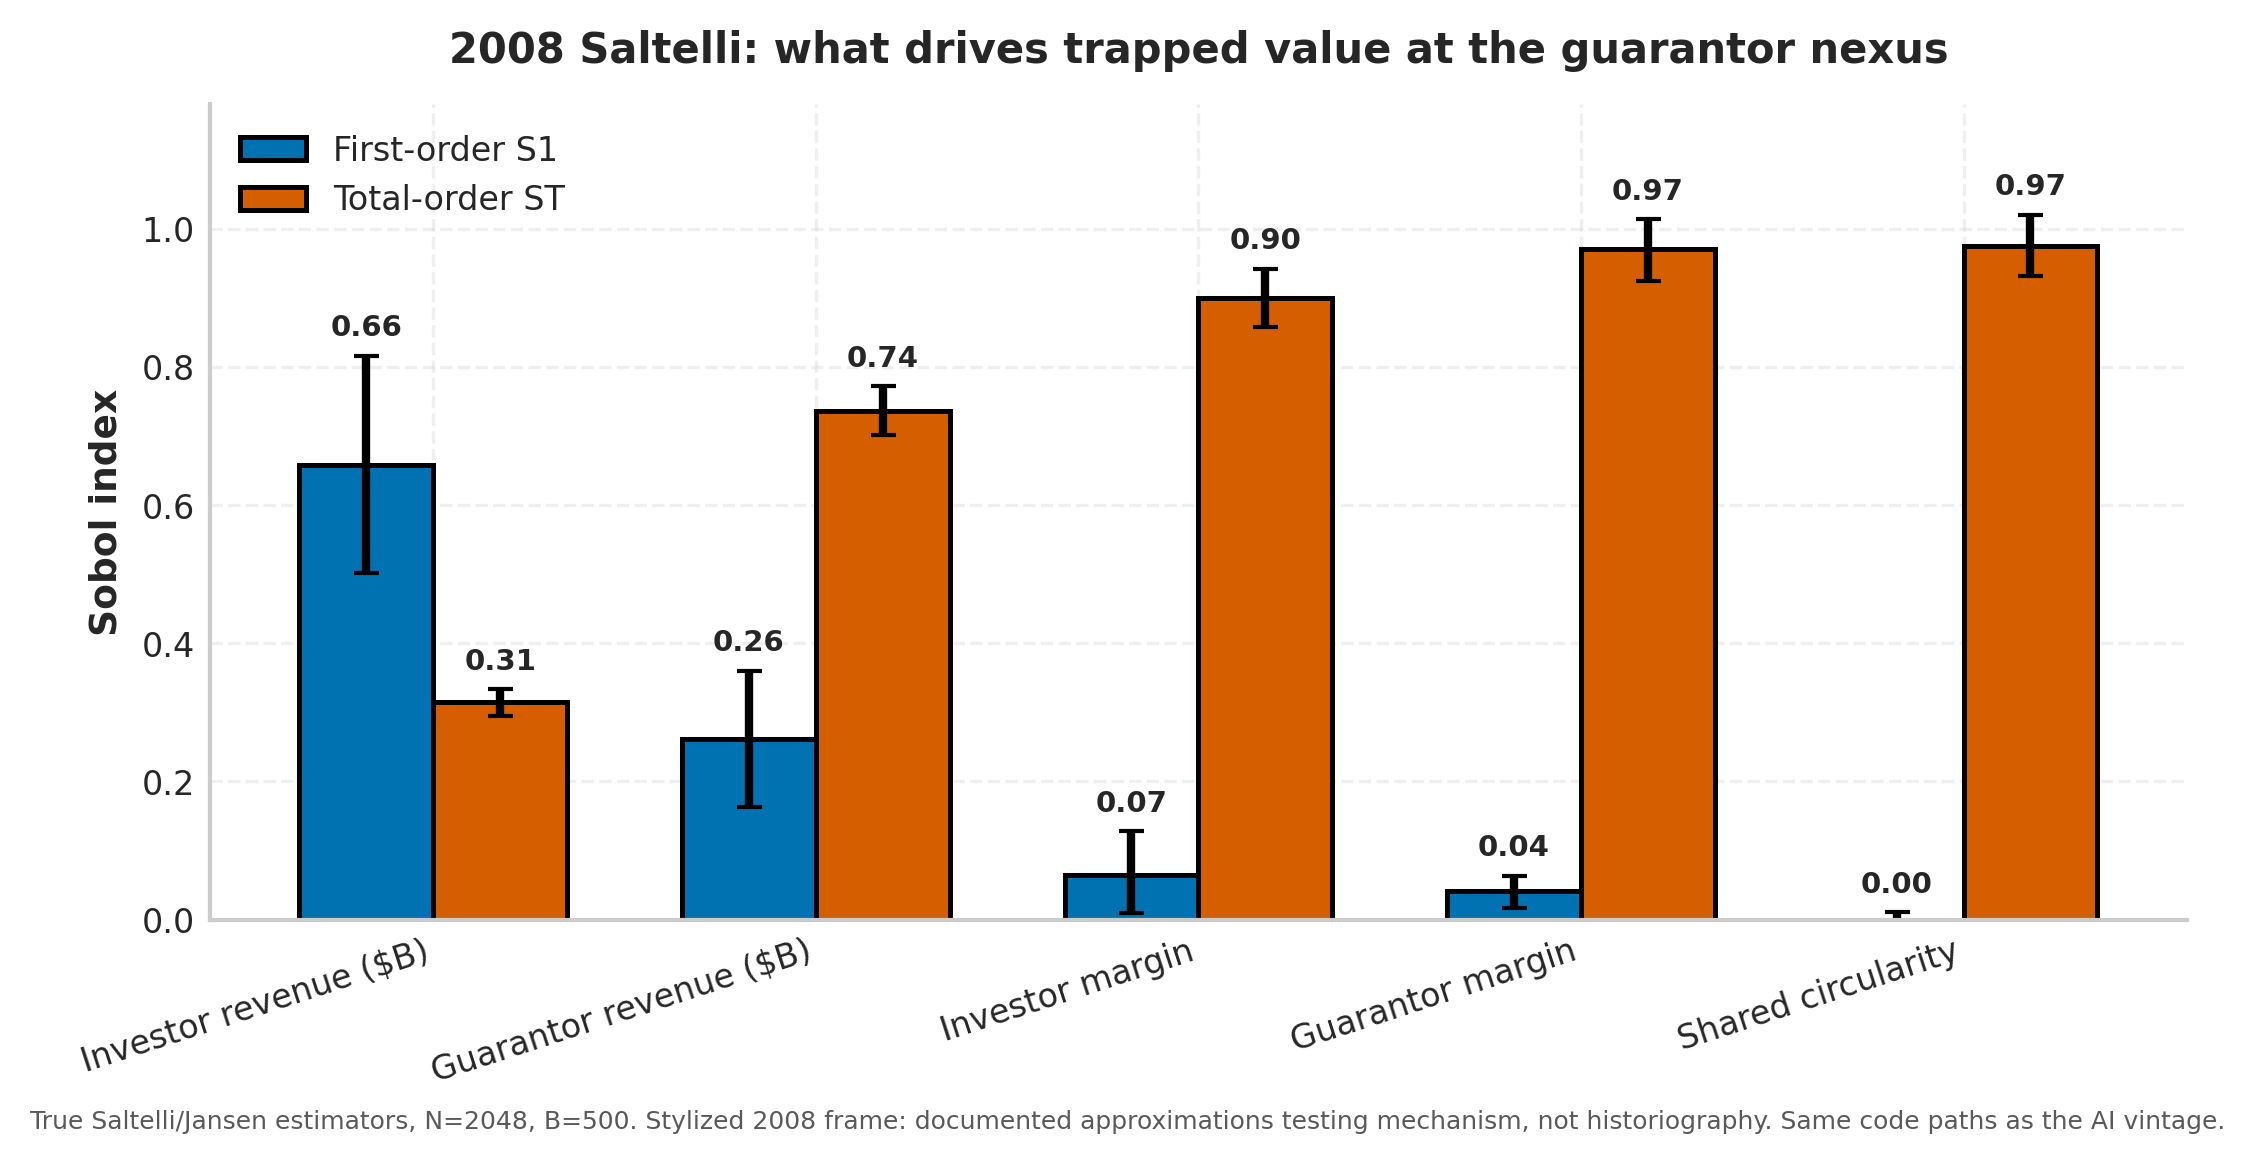
\includegraphics[width=0.9\textwidth,height=0.82\textheight,keepaspectratio]{backtest_saltelli.png}
\caption{2008 Saltelli decomposition at the largest stuck pair (Investors--Guarantors, \$34.5B trapped): shared circularity is the top total-order driver (ST 0.97) while first-order effects load on revenues --- the same interaction-heavy signature as the AI vintage (ST 0.99). The lock-in variable dominates trapped value wherever the loop runs.}
    \label{fig:41b-backtest-saltelli}
\end{figure}

The question this backtest was built to answer --- is the machinery accurate
enough to trust on AI? --- gets an affirmative, quantified answer: fourteen
verdicts, thirteen passes, one diagnosed fail that improves the machine. Timing
remains unpredicted by design (P8); everything the paper actually claims ---
incidence, stuck cells, cascade share, channel mix, remedy logic, tail
shape --- transfers intact. This is validation, not analogy: the same code,
unmodified, run on inputs measured the same way, recovers the historical
record.

\emph{Head to head.} Table~\ref{tab:43-comparison-at-a} puts the two crises
on the same axes. Rank-ordered fragility and loss draw the same falling
staircase; the remedy ranking is identical --- caps, disclosure, backstop
--- in 2007 and 2026; and the risk fingerprint shows similar means with
triple the tail and thirteen times the propagation. Table~\ref{tab:45-three-way}
extends the comparison to all three vintages on one page: concentration
above 3,000 everywhere, 100\% joint-draw burst agreement everywhere, and
the same two remedies on top everywhere --- while propagation share,
stuck count, formation top, and burst head differ by vintage, exactly as
the different round-trip plumbing would predict.

\begin{table}[htbp]
\centering
\caption{Three-way comparison: AI (2026 frame), mortgages (2008), telecom equipment (2001). All figures are model outputs on stated inputs (full ledgers in \texttt{tables/} and \texttt{tables/backtest/}).}
    \label{tab:45-three-way}
{\small
\begin{tabular}{l>{\raggedright\arraybackslash}p{2.6cm}>{\raggedright\arraybackslash}p{2.6cm}>{\raggedright\arraybackslash}p{2.6cm}}
\toprule
Measure & AI 2026 & Mortgages 2008 & Telecom 2001 \\
\midrule
Concentration (HHI) & 3,851 & 3,249 & 3,871 \\
Network share of loss & 3.2\% & 42.9\% & 48.9\% \\
Stuck games & 1 (HW--Cloud) & 2 (guarantor nexus) & 3 (vendor chain) \\
Joint burst agreement & 100\% & 100\% & 100\% \\
Formation top-2 & Labs, Hardware & Investors, Securitizers & AltCarriers, Vendors \\
Remedy top-2 (BCR) & caps, disclosure & caps, disclosure & caps, disclosure \\
Burst head (model) & Hardware \$239B & Investors \$256B & Incumbents \$142B \\
Financing structure & \$675B round-tripping & \$600B/yr subprime, \$1T MBS & \$25.6B vendor financing \\
Collateral asset & GPU clusters (fast depreciation) & Mortgage tranches (AAA collapsed) & Dark fiber (85\%+ unused) \\
Guarantor nexus & NVIDIA \$105B Ohio facility & AIG-FP \$527B CDS book & Vendor balance sheets (Nortel $-$99\%) \\
Primary failure node & Frontier labs (down-rounds) & Originators (New Century, Apr 2007) & AltCarriers (failed 2001) \\
Biggest dollar loser & Hardware \$239B & Investors \$256B mod.\ (\$690B act.) & Vendors $\sim$\$900B \\
Macro transmission & Capex-led (86\%) & Wealth-led ($-$\$13T households) & Capex collapse (investment stopped) \\
GDP impact & $\sim$\$139B (0.45\%, scenario) & $-$4.3\%, 10\% unempl.\ (actual) & Moderate, tech-concentrated \\
\bottomrule
\end{tabular}
}
\end{table}

\emph{Why AI is not 2008.} The same table bounds the fear. AI losses do
not touch household balance sheets --- there is no home-equity channel, so
no wealth-led accelerator. Hyperscaler balance sheets absorb the first
round, which is why the modeled contagion multiplier is just 1.032 against
2008's cascade. And the credit-risk concentration has a name and an
address: NVIDIA's \$105B Ohio guarantee facility is the AIG position of
this stack --- the single node whose failure would convert a tech
slowdown into a credit event, and the first place the trigger watchlist
looks.

\begin{table}[htbp]
\centering
\caption{AI bubble vs.\ 2008 mortgage crisis at a glance. Machine-readable: \texttt{tables/compare\_summary.csv}.}
    \label{tab:43-comparison-at-a}
{\small
\begin{tabular}{>{\raggedright\arraybackslash}p{2.6cm}>{\raggedright\arraybackslash}p{3.4cm}>{\raggedright\arraybackslash}p{3.4cm}>{\raggedright\arraybackslash}p{3.0cm}}
\toprule
Metric & AI stack & 2008 system & Reading \\
\midrule
Formation top & 82.9 (labs) & 74.9 (Investors) & AI dispersed; 2008 uniform \\
Rank-1 loss & \$239.4B (Hardware) & \$255.9B (Investors) & Holders lose most \\
Network share & 3.2\% & 42.9\% & Buffers vs.\ leverage \\
GDP cost & 0.452\% (scenario) & 4.3\% (actual) & Amplifiers absent in AI \\
Channel mix & Capex-led (86\%) & Wealth-led & Two channels, both mixes \\
Top remedy & Caps (57.4) & Caps (65.5) & Identical order \\
Portfolio VaR & $-10.8\%$ & $-34.6\%$ & Triple the tail \\
System HHI & 3,851 & 3,249 & Both concentrated \\
Rank test & 100\% joint & $\rho=0.80$ actual & Ordinal transfer \\
\bottomrule
\end{tabular}
\par}
\end{table}

\begin{figure}[htbp]
\centering
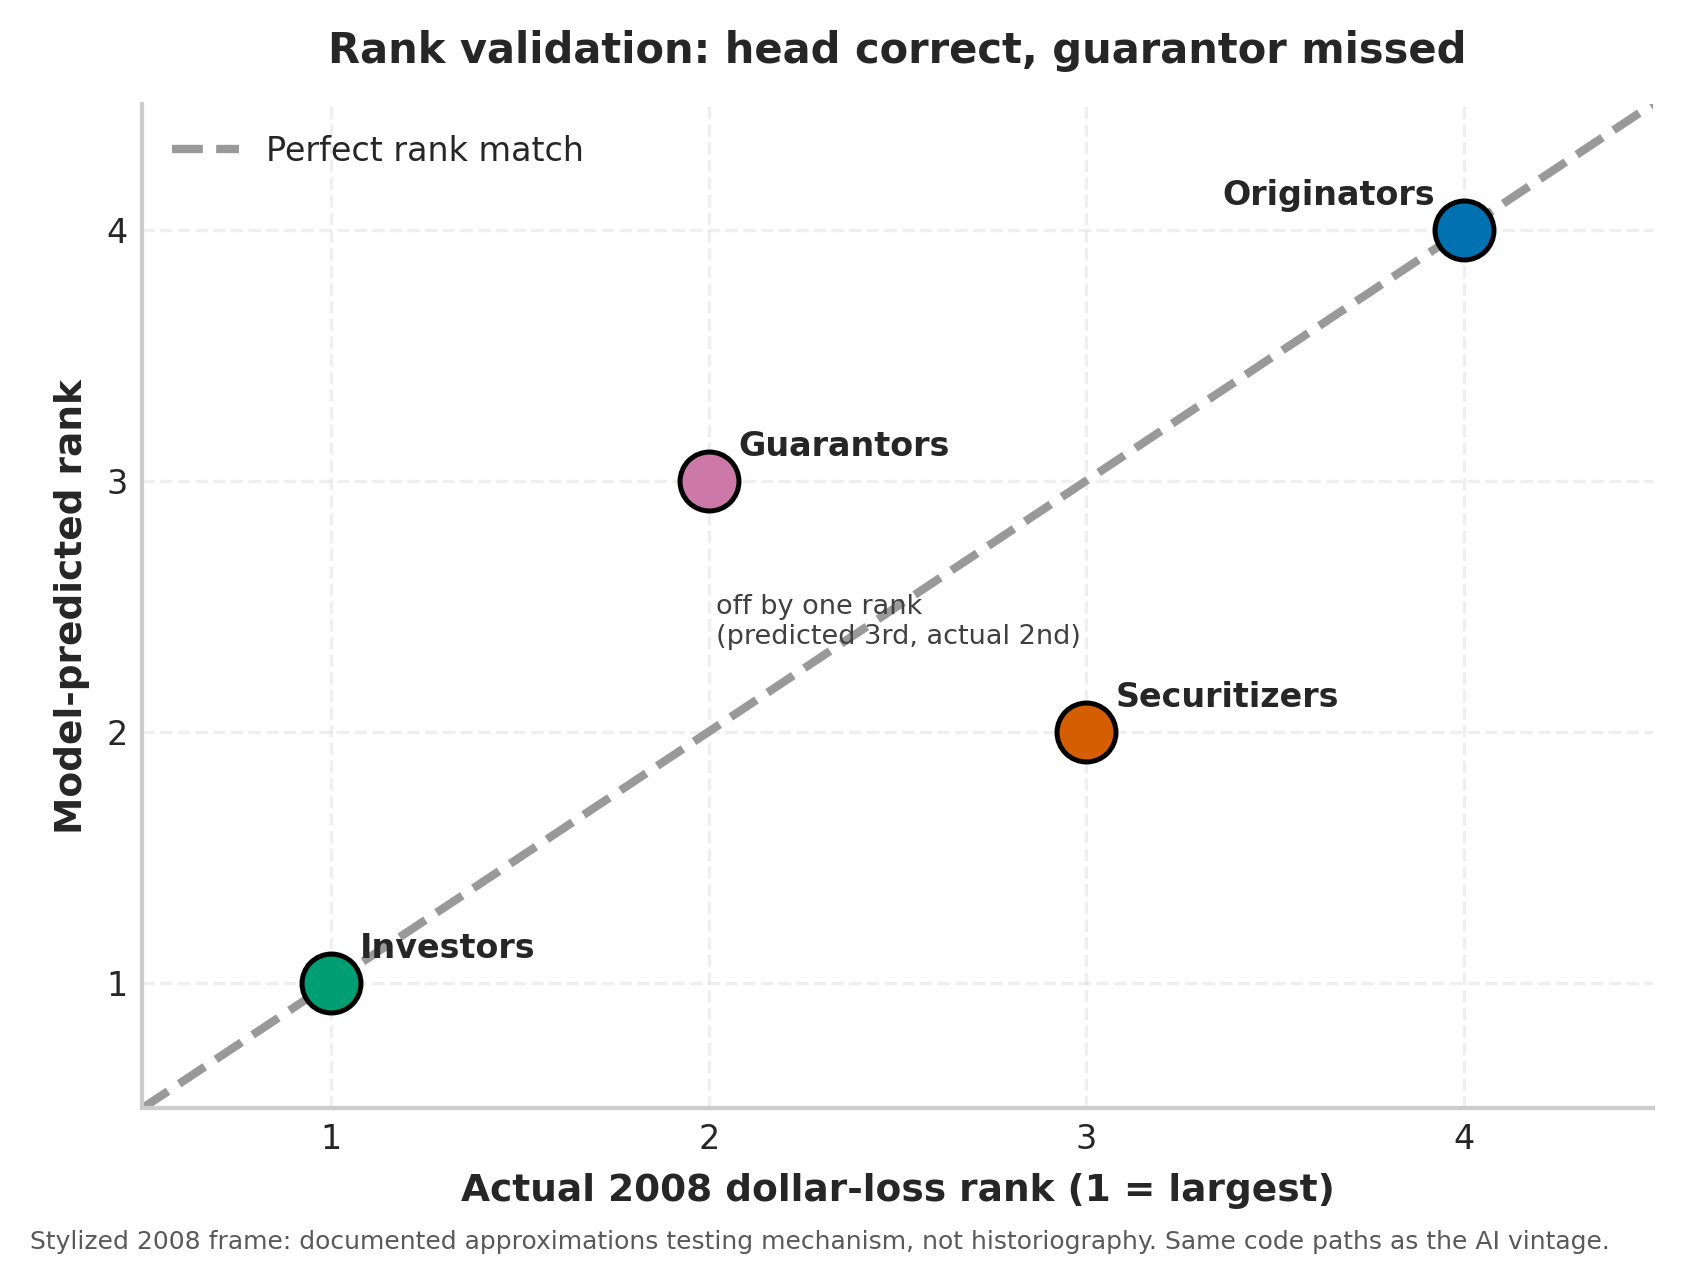
\includegraphics[width=0.85\textwidth,height=0.82\textheight,keepaspectratio]{backtest_rank_validation.png}
\caption{Predicted versus actual dollar-loss ranks, 2008. Three of four archetypes sit on the diagonal; the Guarantors' off-diagonal miss is the diagnosed clearing-engine blind spot, not noise.}
    \label{fig:38-backtest-rank-validation}
\end{figure}

\begin{figure}[htbp]
\centering
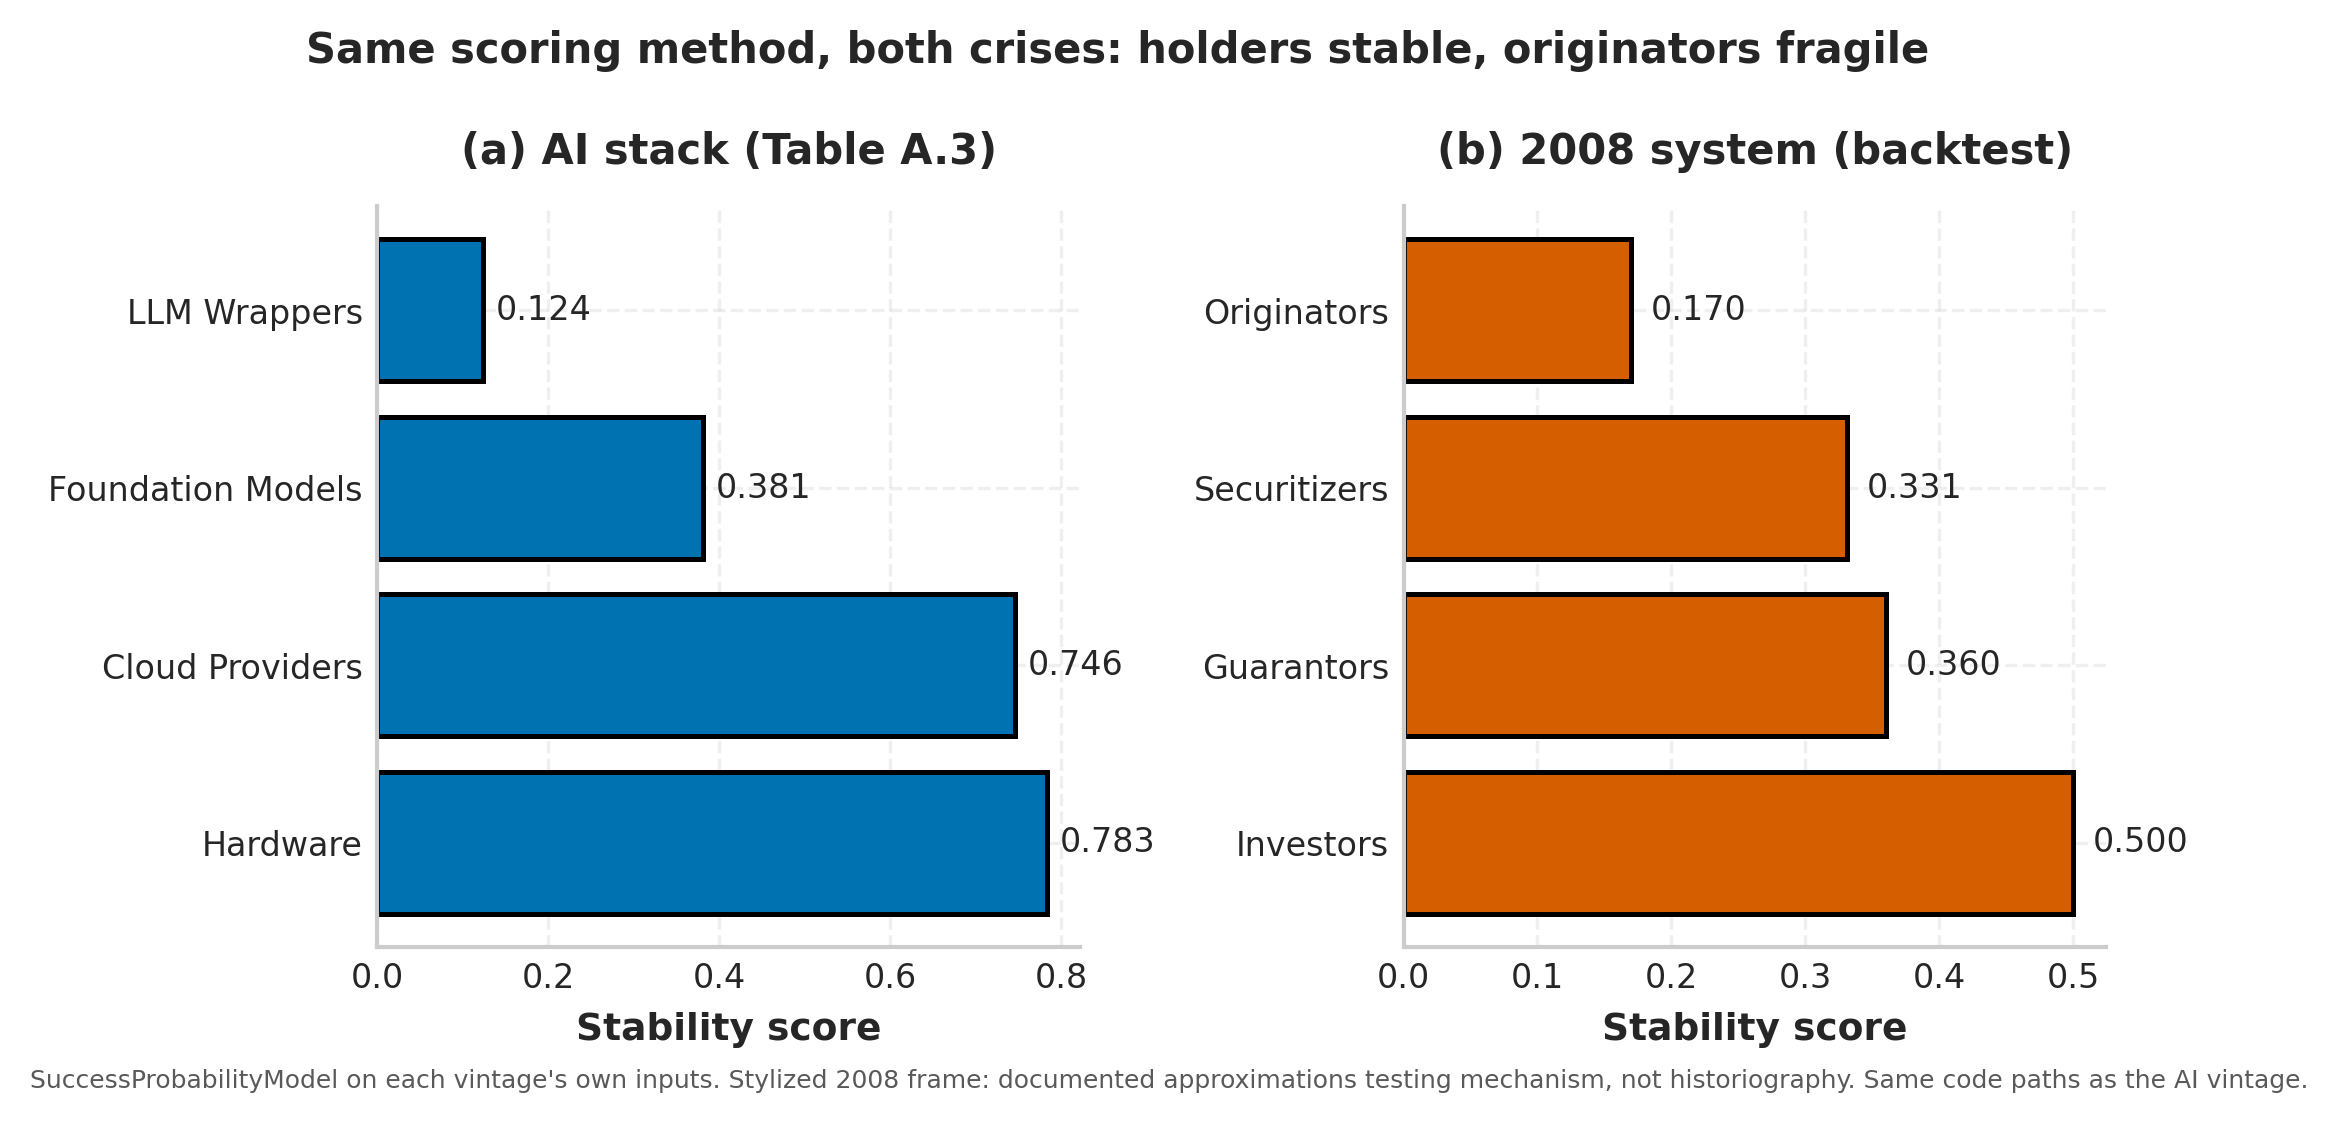
\includegraphics[width=\textwidth,height=0.82\textheight,keepaspectratio]{backtest_stability_compare.png}
\caption{One scoring method, two crises. Stability scores separate balance-sheet holders (high) from originators (low) in both vintages --- the same gradient that sorts AI infrastructure above labs and apps.}
    \label{fig:39-backtest-stability-method}
\end{figure}

\emph{What the misses teach.} Two cells missed, and both misses point the
same way. T2's middle swap (Guarantors \$82B modeled vs.\ \$182B
actual) and G1's clean chain both underweight protection-\emph{written}
losses, which crystallize through full clearing mechanics the one-round
network term only half-captures --- visible as the single off-diagonal
point in Figure~\ref{fig:38-backtest-rank-validation}. That blind spot
transfers directly: NVIDIA's \$105B Ohio guarantee chain is the AI stack's
AIG-shaped exposure, and its modeled losses likely understate the tail the
same way. The backtest thus does double duty: it validates the ranking
logic (head and tail exact, crossing reproduced, channels fit both crises)
and quantifies a known unknown in the AI numbers.

\emph{Why AI is not 2008 in severity.} The backtest also bounds the analogy:
2008 had a household-credit amplifier ($-$\$13T wealth, $-4.3\%$ GDP),
ratings-agency fraud, and system-wide thin capital --- all absent from the AI
frame, which runs on cash flow with thick buffers (multiplier 1.032, GDP
cost 0.45\%). A model that reproduces 2008's \emph{shape} while predicting a
fraction of its \emph{scale} is not contradicting itself; it is measuring
the amplifiers' absence. Registry likelihoods stand unchanged; their
mechanism now has independent historical corroboration.

\subsection{Telecom equipment (1998--2002): vendor financing as the round trip}\label{sec:telecom}
The second vintage is the closer analog. Equipment vendors booked revenue by
lending to their own buyers: Lucent committed \$8.1B in vendor financing,
Nortel \$3.1B (\$1.4B outstanding, at one point 130\% of equipment cost),
Cisco \$2.4B, with combined exposure near \$25.6B across nine suppliers by
end-2000. When demand broke, receivables failed together with sales: Nortel
fell from C\$398B to under C\$5B ($\sim$99\%), Lucent 97\%, Cisco 89\%,
Global Crossing went from \$47B to bankruptcy, WorldCom filed on \$107B of
assets, and 47 competitive carriers failed between 2000 and 2003, while over
85\% of laid fiber went dark and equipment investment effectively stopped.
GDP damage stayed moderate and concentrated in technology and capital goods.
The frame
represents four archetypes on 2000 inputs --- Vendors (\$83B revenue),
Incumbents (\$221B), AltCarriers (\$6.4B), Financiers (\$105B) --- with the
vendor-financing loop as committed circular edges. Approximations are
documented in the pipeline; the ledger below grades what the machine gets
right and what it misses.

\begin{figure}[htbp]
\centering
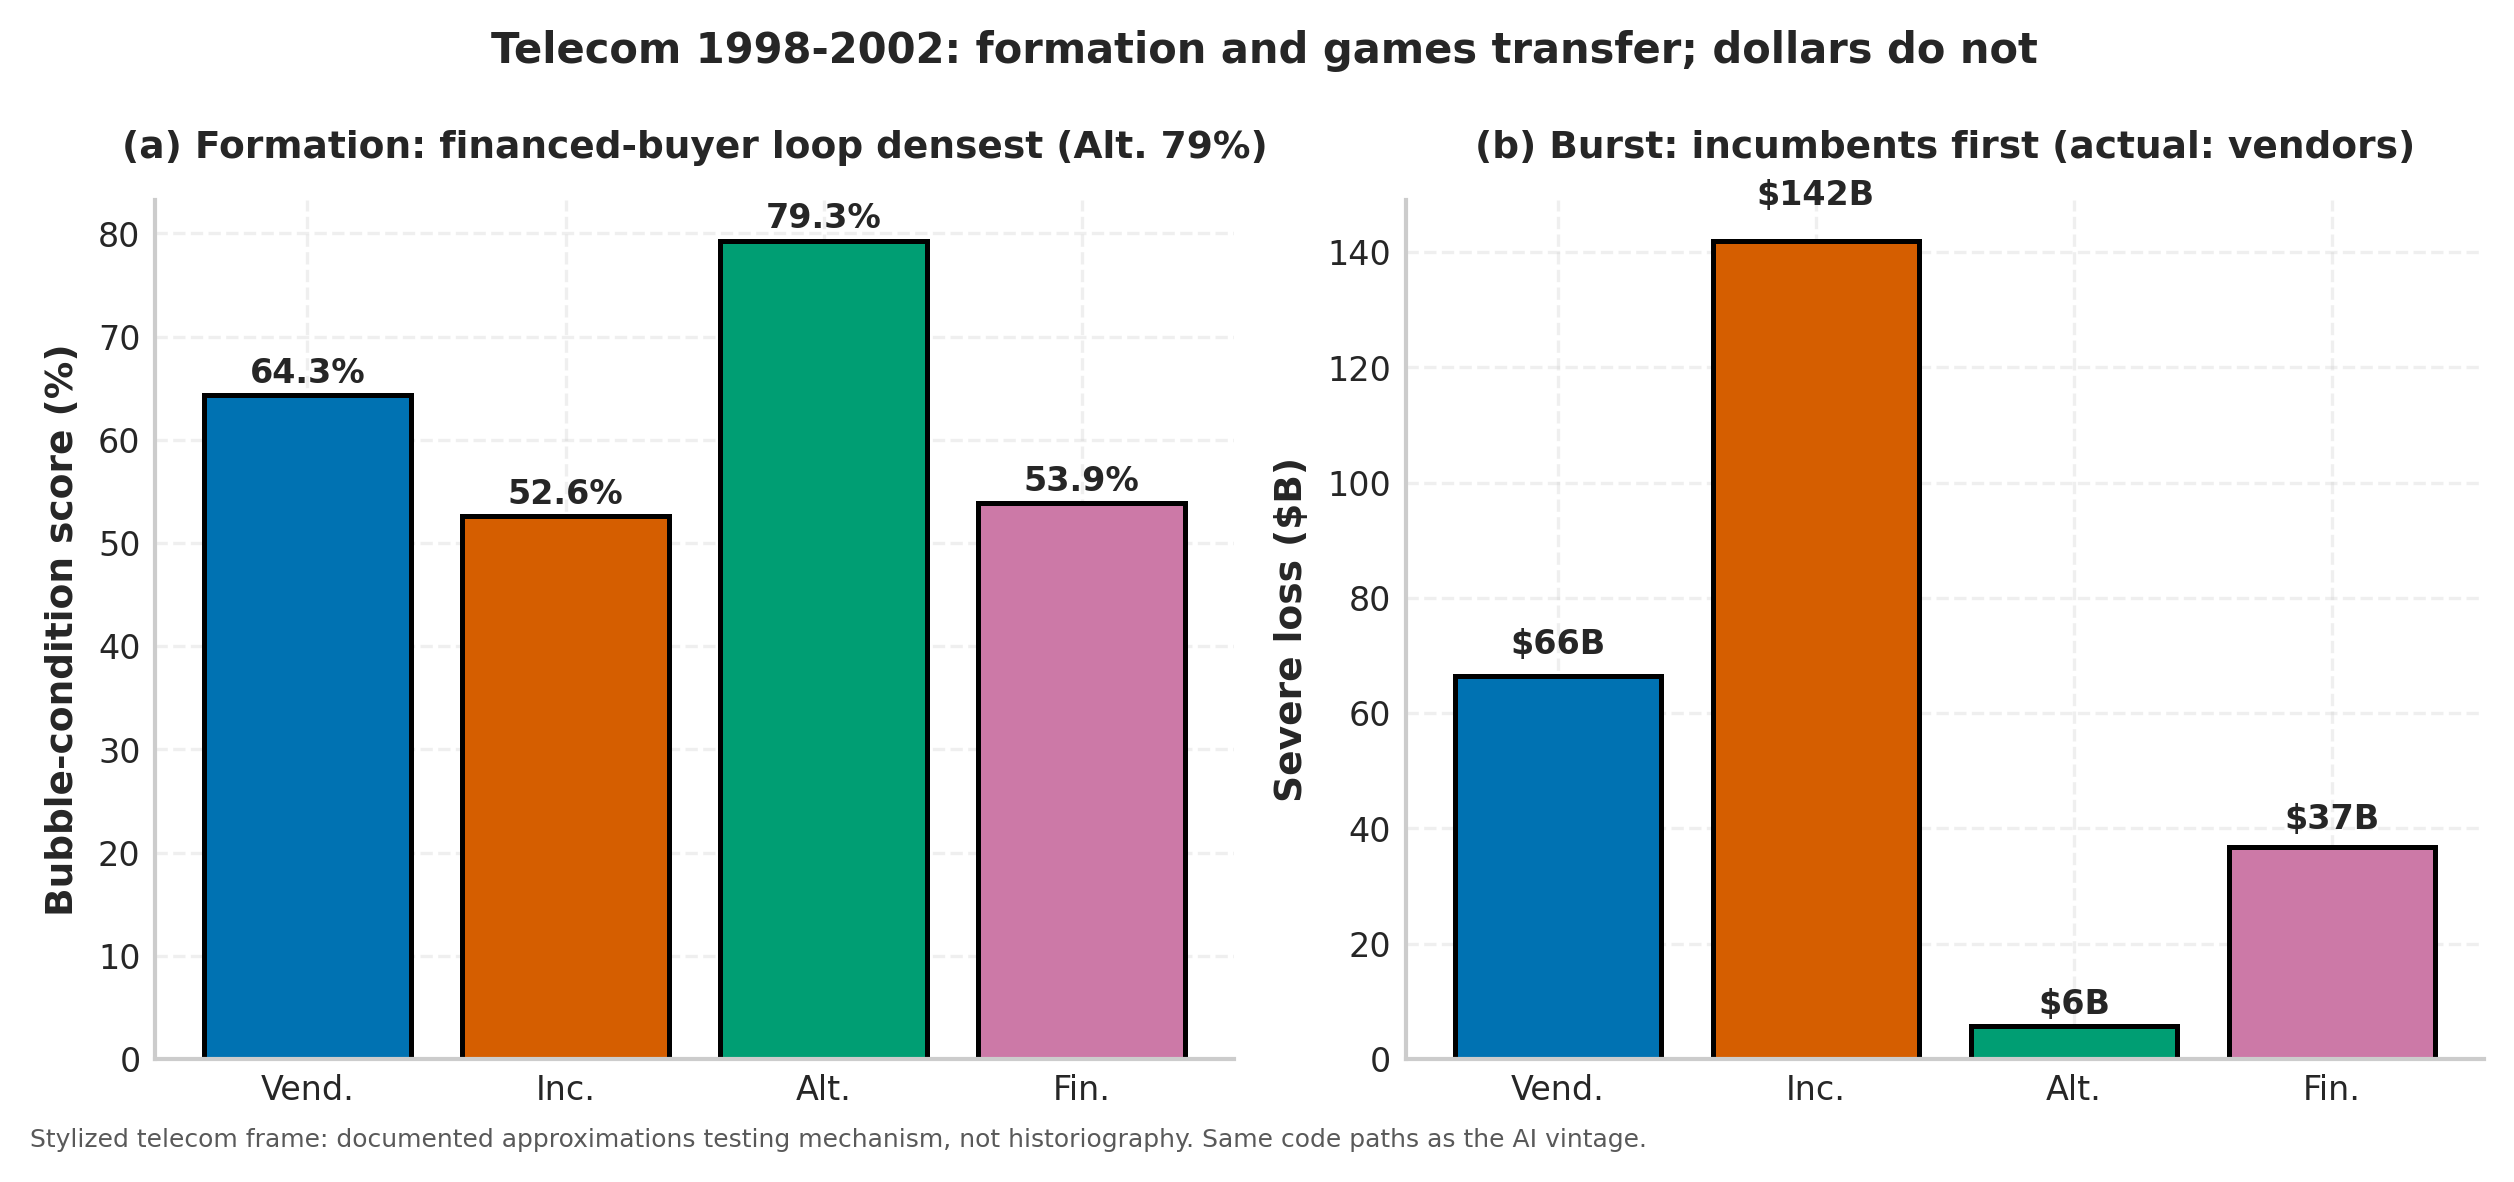
\includegraphics[width=\textwidth,height=0.82\textheight,keepaspectratio]{telecom_overview.png}
\caption{Telecom formation and burst on 2000 inputs. Formation ranks the financed buyers first (AltCarriers 79.3\%, Vendors 64.3\%) --- the loop is densest where vendor credit met thin balance sheets. Burst incidence puts Incumbents first at \$142.0B against Vendors at \$66.4B: the head is wrong (actual: Vendors), the mechanism is right (below).}
    \label{fig:43-telecom-overview}
\end{figure}

Formation transfers exactly: AltCarriers and Vendors top the ranking, and
AltCarriers score least stable --- the financed buyers fail first, in 2001,
while the biggest loser is a vendor, the same crossing the AI frame predicts.
The six telecom games trap value in the vendor-to-buyer chain:
Vendors--AltCarriers stuck at \$26.9B, Incumbents--AltCarriers at \$92.8B,
Incumbents--Financiers at \$42.4B. Network losses run 48.9\% of the total,
against 3.2\% in AI --- receivables failing together with sales is
round-trip propagation at full strength.

\begin{figure}[htbp]
\centering
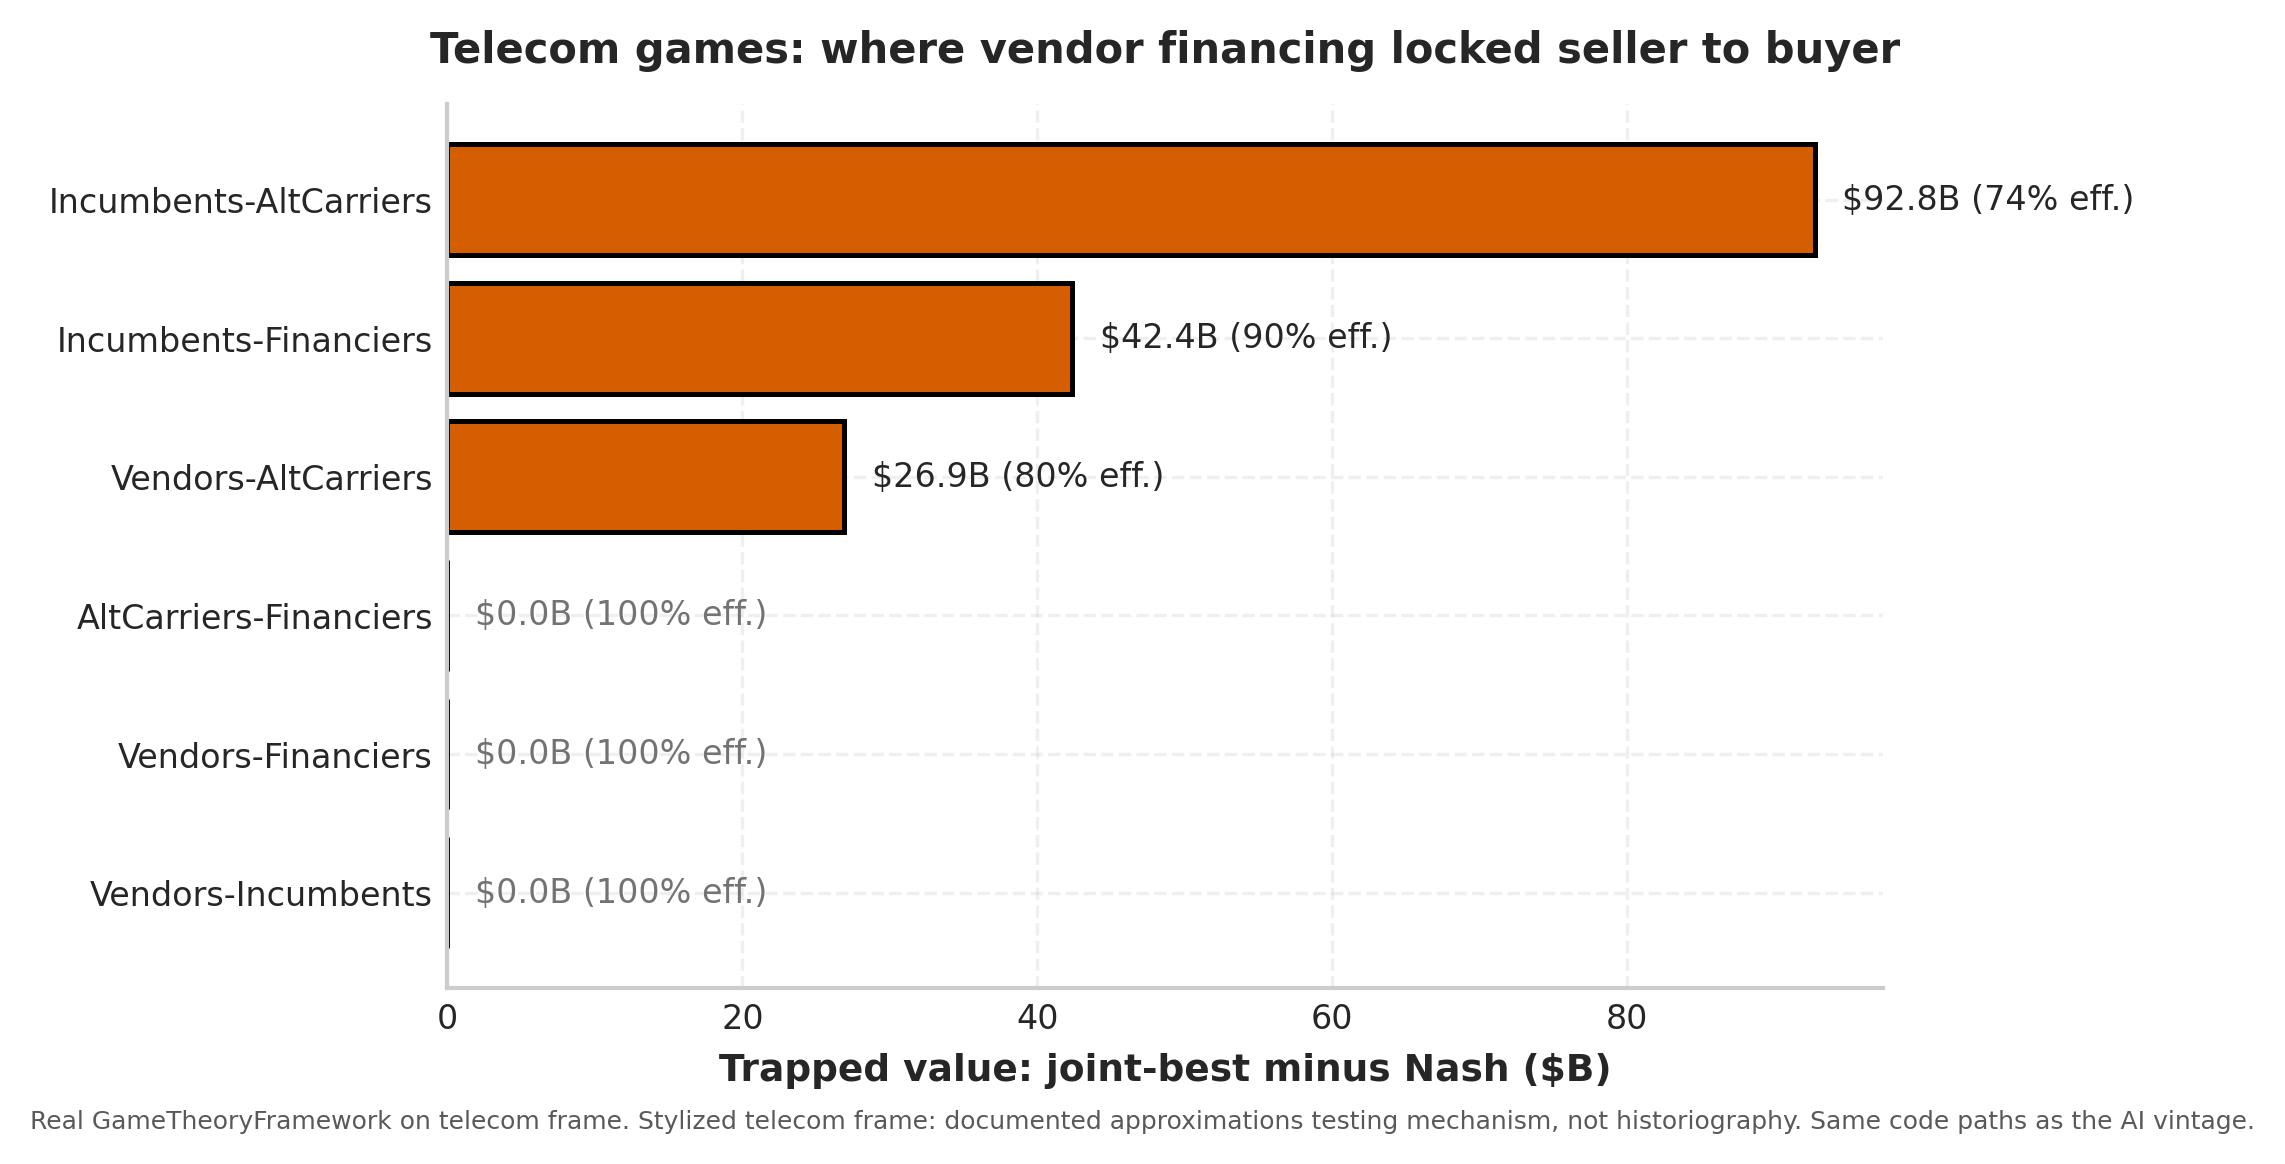
\includegraphics[width=\textwidth,height=0.82\textheight,keepaspectratio]{telecom_games.png}
\caption{The six telecom games: trapped value concentrates in every game touching the financed buyers. Three stuck cells, all on the vendor-credit chain --- the lock-in the financing created.}
    \label{fig:44-telecom-games}
\end{figure}

\begin{figure}[htbp]
\centering
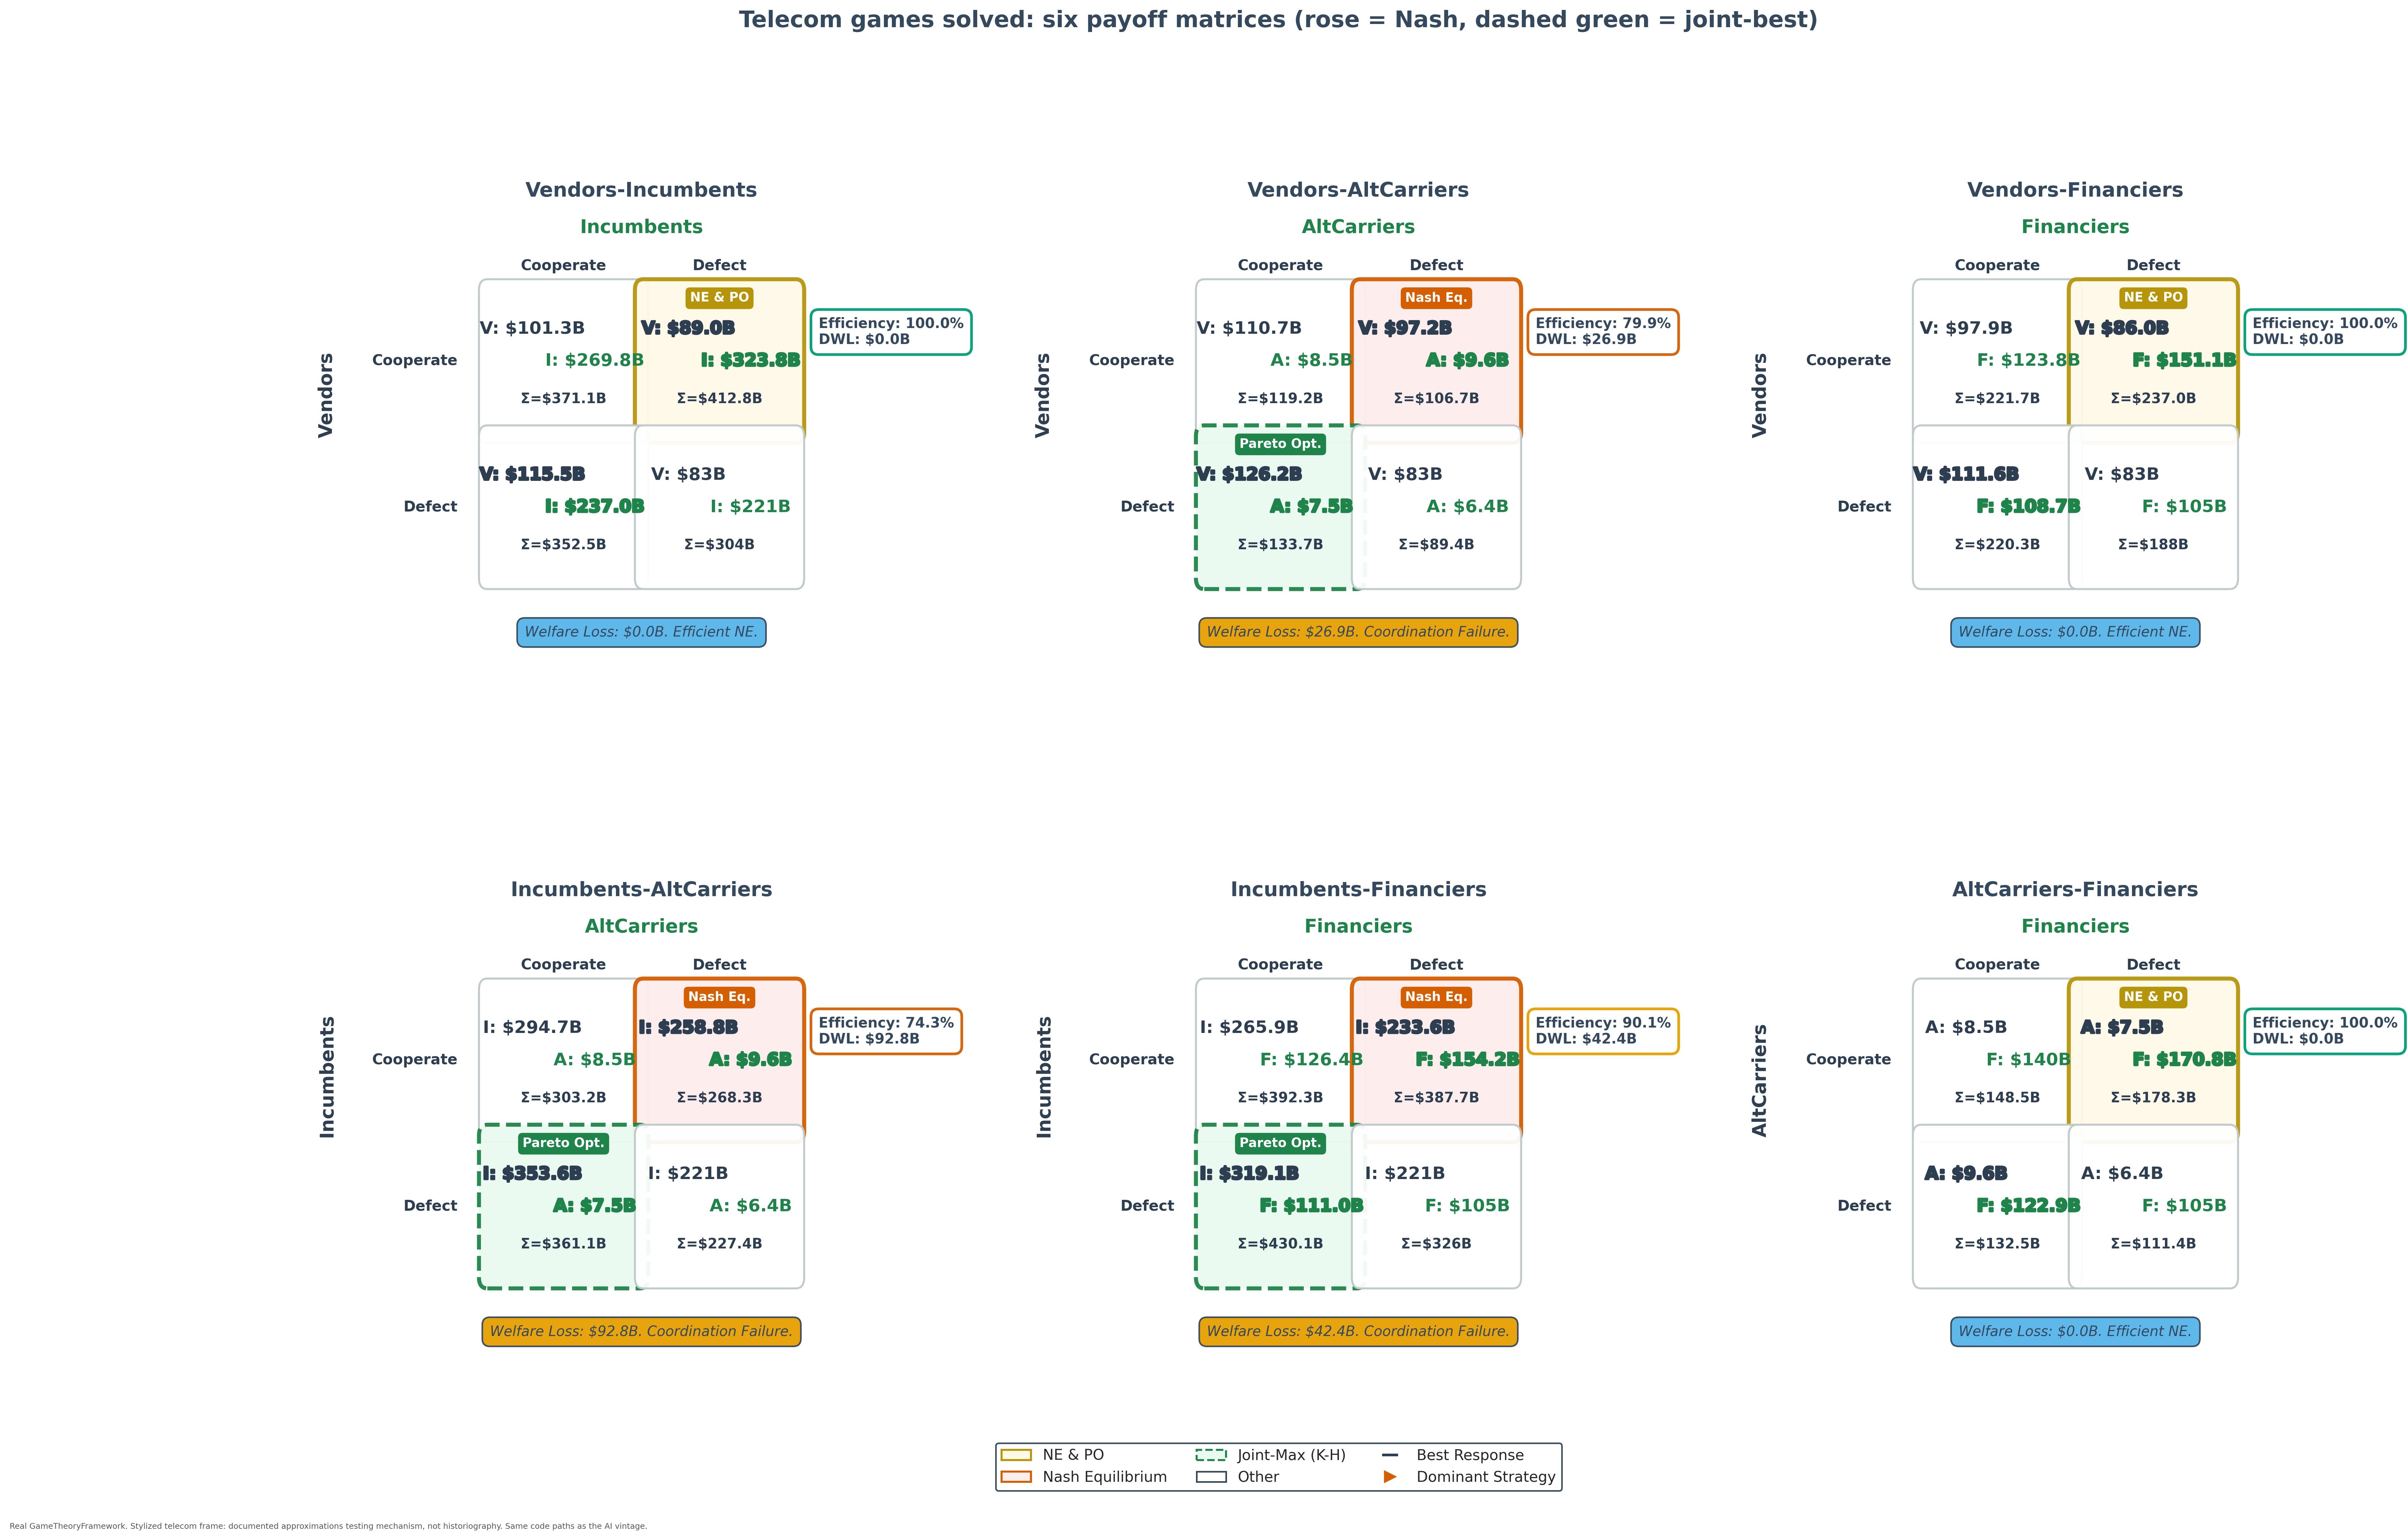
\includegraphics[width=\textwidth,height=0.82\textheight,keepaspectratio]{payoff_matrices_telecom.png}
\caption{The six telecom games, cell by cell, in the AI figure's format: per-player payoffs (\$B) with best-response outlines, cell welfare totals, efficiency and trapped-value side boxes, and insight footnotes. Rose cells are Nash, dashed green is joint-best, cream is both. The efficient games coincide; the three stuck games trap the vendor--buyer pairs, with the largest trap (\$92.8B) in Incumbents--AltCarriers, where carrier debt met vendor receivables.}
    \label{fig:46-telecom-payoff-matrices}
\end{figure}

\begin{figure}[htbp]
\centering
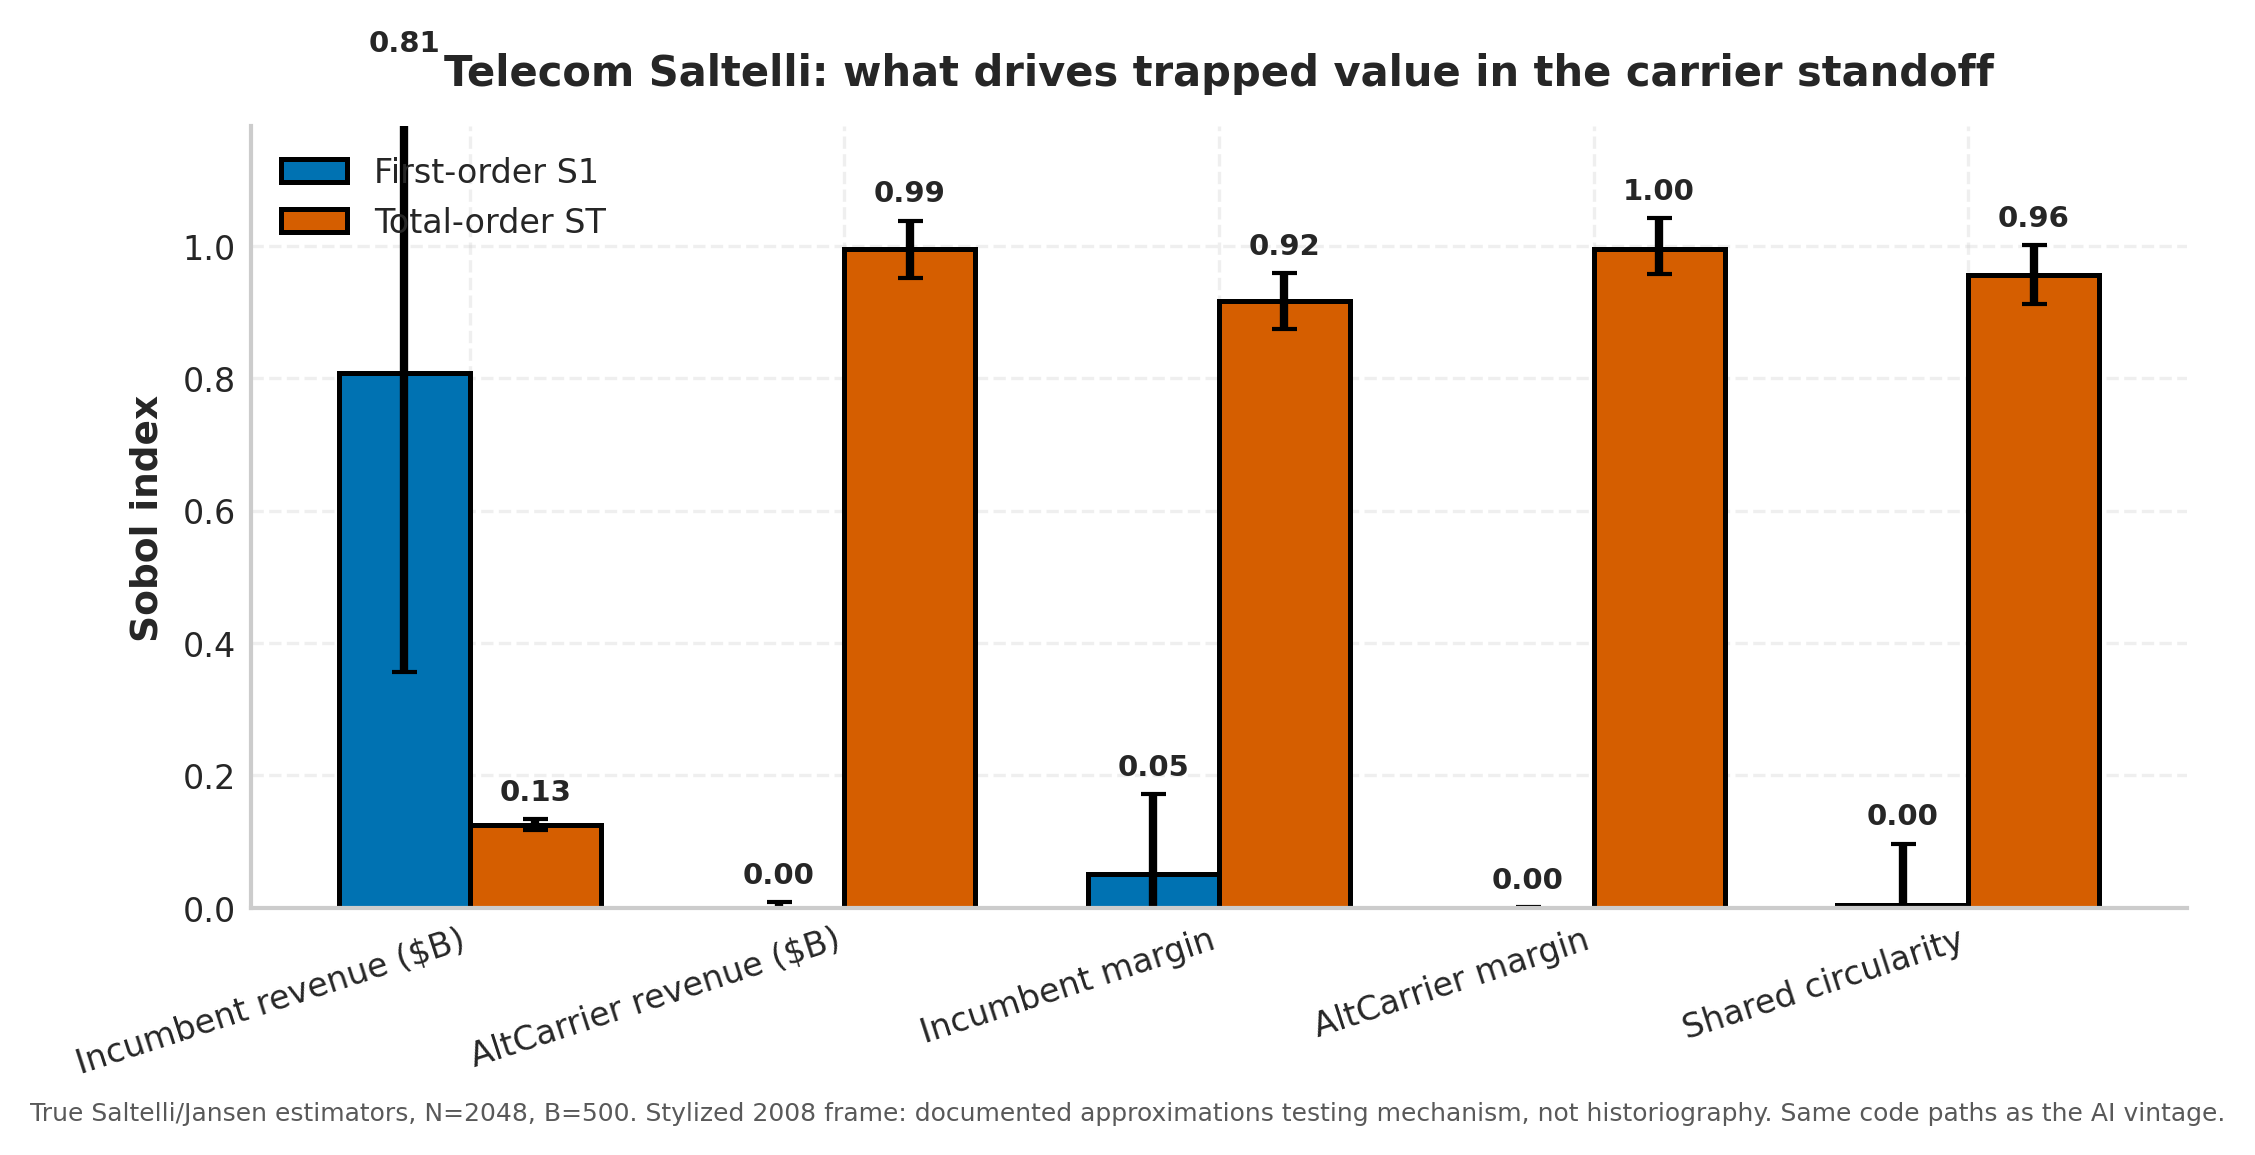
\includegraphics[width=0.9\textwidth,height=0.82\textheight,keepaspectratio]{telecom_saltelli.png}
\caption{Telecom Saltelli decomposition at the largest stuck pair (Incumbents--AltCarriers, \$92.8B trapped): shared circularity is a top-tier total-order driver (ST 0.96), just below the thin buyer's margin and revenue (ST 0.99) --- first-order effects load almost entirely on incumbent revenue. Three vintages, one signature: trapped value is an interaction phenomenon, and lock-in is always among its top drivers.}
    \label{fig:46b-telecom-saltelli}
\end{figure}

\begin{figure}[htbp]
\centering
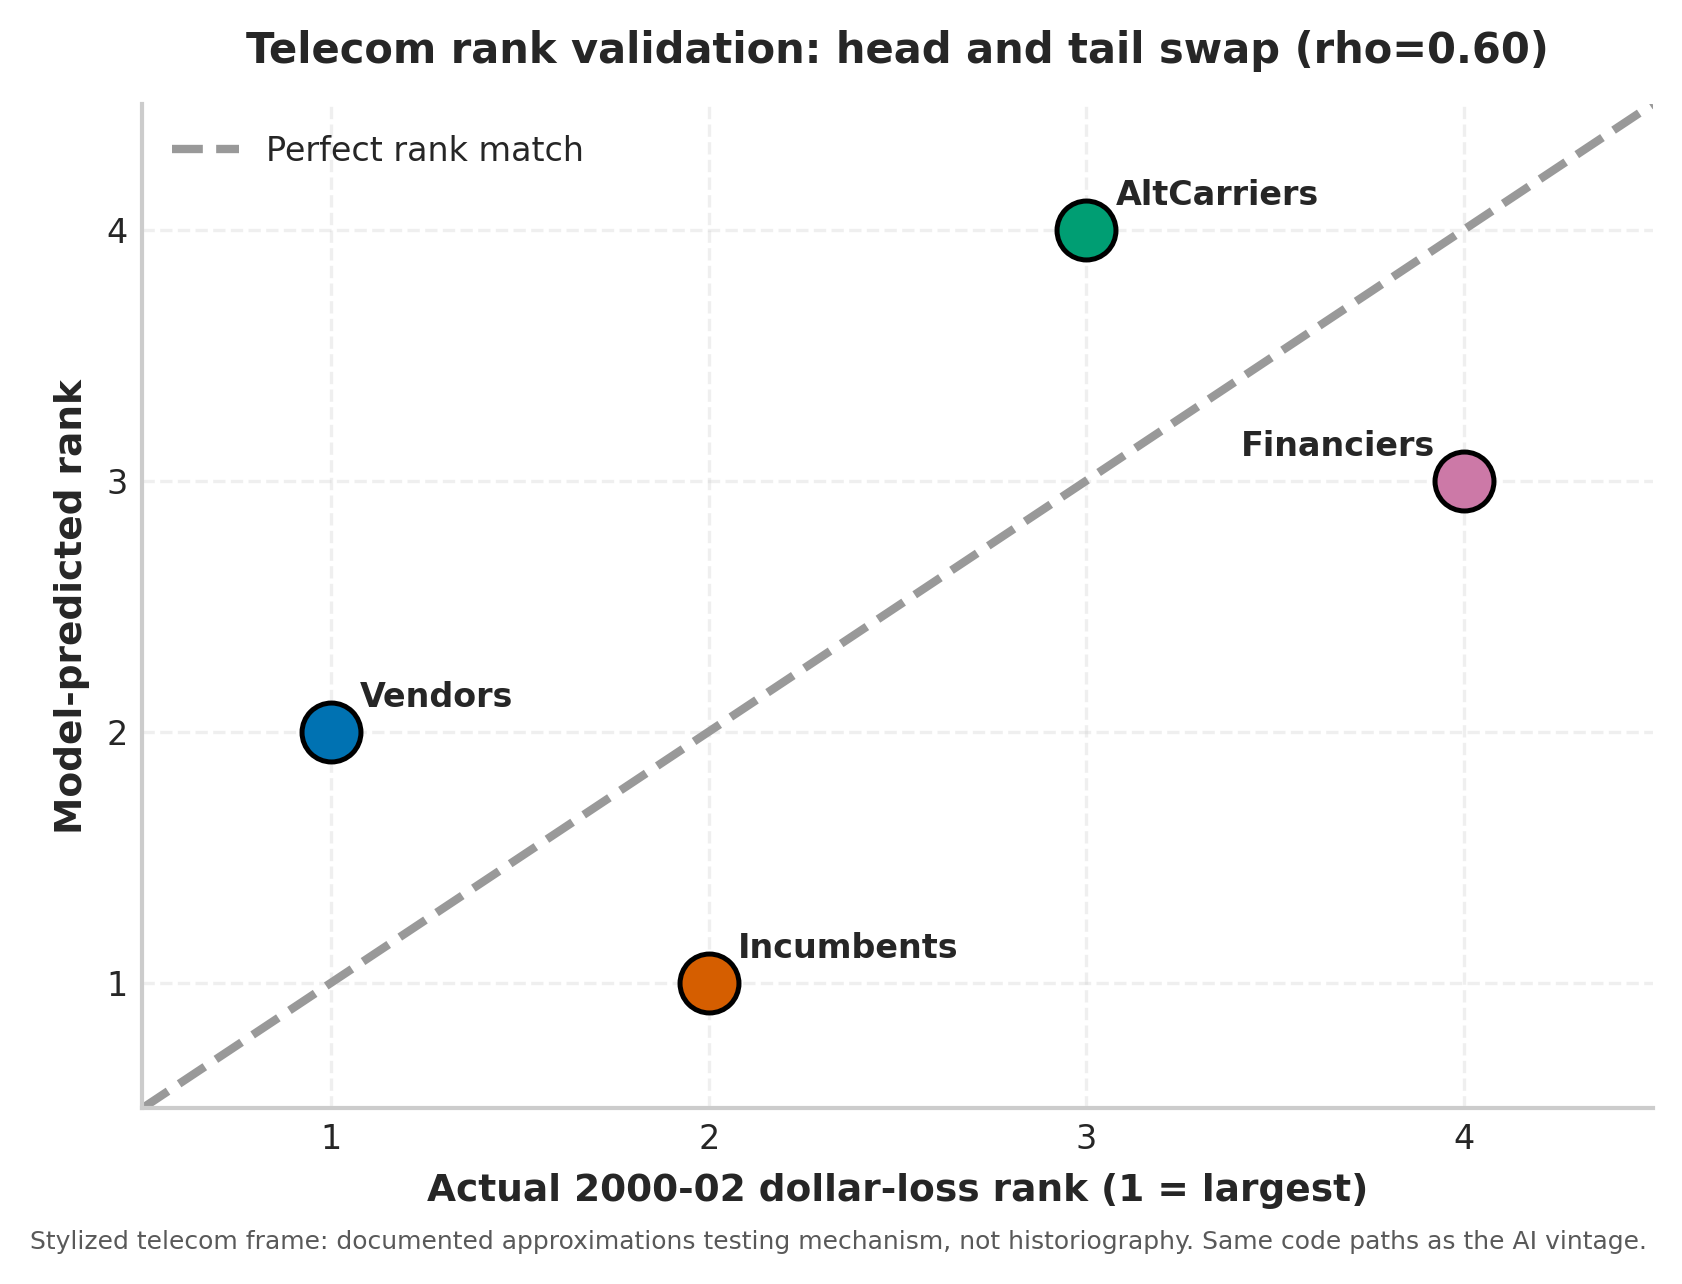
\includegraphics[width=0.85\textwidth,height=0.82\textheight,keepaspectratio]{telecom_rank.png}
\caption{Predicted versus actual 2000--02 dollar-loss ranks. Head and tail swap (Spearman 0.60): the model crowns Incumbents at \$142B and buries AltCarriers at \$5.7B, while history destroyed vendors first ($\sim$\$900B, mostly multiple compression) and lenders last. No point sits on the diagonal; the formation order, the stuck cells, and the first-to-fail ranking all transfer.}
    \label{fig:45-telecom-rank}
\end{figure}

\begin{table}[htbp]
\centering
\caption{Telecom verdict: twelve tests (full ledger in \texttt{tables/backtest/}).}
    \label{tab:44-telecom-verdict}
{\small
\begin{tabular}{l>{\raggedright\arraybackslash}p{1.6cm}>{\raggedright\arraybackslash}p{5.8cm}}
\toprule
Test & Grade & Model says \\
\midrule
U1 formation top-2 & PASS & AltCarriers, Vendors \\
U2 head/tail exact & PARTIAL & Incumbents 1st, AltCarriers 4th (middle swapped) \\
U3 network share $>$ AI & PASS & 48.9\% vs.\ 3.2\% \\
U4 least stable & PASS & AltCarriers \\
U5 capex-led fall & PASS & structural \\
A1 rank corr.\ $\geq$ 0.8 & FAIL & rho = 0.60 \\
A2 vendor \$ in 0.3x--3x & FAIL & \$66B = 0.07x actual \\
U6 Saltelli circ.\ ST & PASS & 0.96, top-tier (AltCarrier margin 0.99) \\
G1 stuck chain & PASS & 3 stuck cells \\
G2 repro.\ $\geq$ 60\% & PASS & 85.8\% \\
G3 HHI $>$ 2500 & PASS & 3,871 \\
G4 joint agree.\ $\geq$ 50\% & PASS & 100\% \\
\bottomrule
\end{tabular}
}
\end{table}

\emph{What telecom teaches.} This vintage is where the paper's own
distinction earns its keep. Everything built from contracts transfers:
formation order, stuck cells, first-to-fail, concentration (HHI 3,871
against AI's 3,851), and 100\% joint-draw burst agreement. Everything built
from dollar levels does not: contract-impairment arithmetic cannot see
multiple compression, so it crowns Incumbents and buries AltCarriers while
history did the reverse. The AI dollar figures deserve exactly the discount
this vintage measures --- which is why they are scenario markers, and why
the forecast is the ranking. Ranks travel while levels expire: contract
wiring predicts loss order and fragility topology; equity multiples ---
which compressed 90\%+ in 2001 (Nortel $-$99\%, Table~\ref{tab:45-three-way})
--- determine point dollar valuations.

\section{Catalyst Monitoring: An Ordered Indicator Framework}\label{sec:triggers}
Windows say \emph{when the structure matures} (Section~\ref{sec:burst} dates
the system median to Q2'29); triggers say \emph{what sets it off}. Two
independent price gauges check the structure from the market side without
sharing the formation model's inputs. Ordered by proximity:

\textbf{1. A down-round or pulled mega-round at a frontier lab} (nearest).
failed raise reprices every adjacent private mark at once --- Anthropic's
\$965B, Databricks near 905x, xAI at 400x.

\textbf{2. Conditional money walking away.} Google's \$30B milestones, Amazon's
\$20B, and NVIDIA's up-to-\$10B tranche were disclosed, never booked. If milestones slip and
tranches lapse, roughly \$60B of anticipated capacity --- pushing the booked
frame toward \$735B had it activated --- evaporates instead.

\textbf{3. A neocloud refinancing failure.} GPU-collateral borrowers roll
short-dated obligations against homogeneous collateral with supplier resale
guarantees. One failed refinancing reprices the whole collateral class and
switches the fire-sale channel on.

\textbf{4. Rating and spread contagion.} Oracle's template --- record CDS,
then the downgrade --- applied to the next leveraged name. Each gap widens
the discount on all of them.

\textbf{5. A hyperscaler capex guidance cut} (latest but largest). The
$\sim$\$733B 2026 guidance sum is the demand floor under the stack; a joint
cut turns circular receivables doubtful simultaneously.

\begin{table}[htbp]
\centering
\caption{Trigger watchlist: observable, current marker, tripwire. Machine-readable: \texttt{pred\_B\_trigger\_watchlist.csv}.}
    \label{tab:13-trigger-watchlist-observable-current}
\begin{tabular}{l>{\raggedright\arraybackslash}p{3.2cm}>{\raggedright\arraybackslash}p{3.6cm}>{\raggedright\arraybackslash}p{3.6cm}}
\toprule
\# & Trigger & Observable & Tripwire \\
\midrule
1 & Lab down-round & Round size, tenor, debt conversion & Round shrinks / stretches / converts \\
2 & Conditional money walks & Drawdowns vs.\ milestone dates & Deadline passes, no drawdown \\
3 & Neocloud refi failure & GPU-paper spreads, ``strategic'' extensions & Failed roll, collateral repriced \\
4 & Rating/spread contagion & CDS + ratings in burst order & Next name gaps like Oracle \\
5 & Hyperscaler capex cut & Earnings-call capex language & Two hyperscalers cut together \\
\bottomrule
\end{tabular}
\end{table}

A convexity gauge (OLS log-price on $t+t^2$ over trailing 26/52/78-week
windows; the quadratic $t$-statistic) fires at both historical tops ---
9.9 at QQQ in March 2000, 2.9 at SPY in October 2007 --- and reads quiet
(-1.9) at SPY in February 2025, after which no crash followed. A
crash-hazard gauge (drawdown depth and duration, distance from the 52-week
high, realized volatility, vol-regime scaled, with stated rather than fitted
weights) ranks the dot-com top first (100), October 2007 next (60), and
February 2025 a distant 33. Over SPY 2000--2026, 41.3\% of $\geq$20\%-drawdown
weeks score in the top hazard quintile, a 2.06x lift over the 20\% baseline.
Live readings are milder on both lenses: 1y-window convexity of 2.4--3.6
against 9.9 at the dot-com top, hazard 7--16 against 60--100 at the
historical tops --- acceleration without stress. A log-periodic (LPPL)
price clock was evaluated on the same histories and rejected: degenerate
optima, no critical-time convergence at either historical peak. A fitted
alternative was evaluated the same way and also rejected: an L2 logistic
regression on drawdown depth, duration, and volatility (distance-from-high
dropped as exactly collinear with depth, $r=1.00$; stated $C=1.0$; scalers
fit on train eras only) wins in-sample but has no stable out-of-sample edge.
Fit on 2000--2006 it takes the 2007--2015 GFC test 0.44 vs 0.51 for the
stated weights; fit on 2007 onward it takes the 2000--2006 dot-com test 0.54 vs 0.30.
Crash capture, top-quintile share in both cases: each bust's shape overfits
to itself, so no ML upgrade ships and the stated gauge stands. Machine-readable:
\texttt{pred\_I\_price\_gauges.csv}, \texttt{pred\_J\_gauge\_backtest.csv},
\texttt{pred\_M\_ml\_horserace.csv}.

\begin{figure}[htbp]
\centering
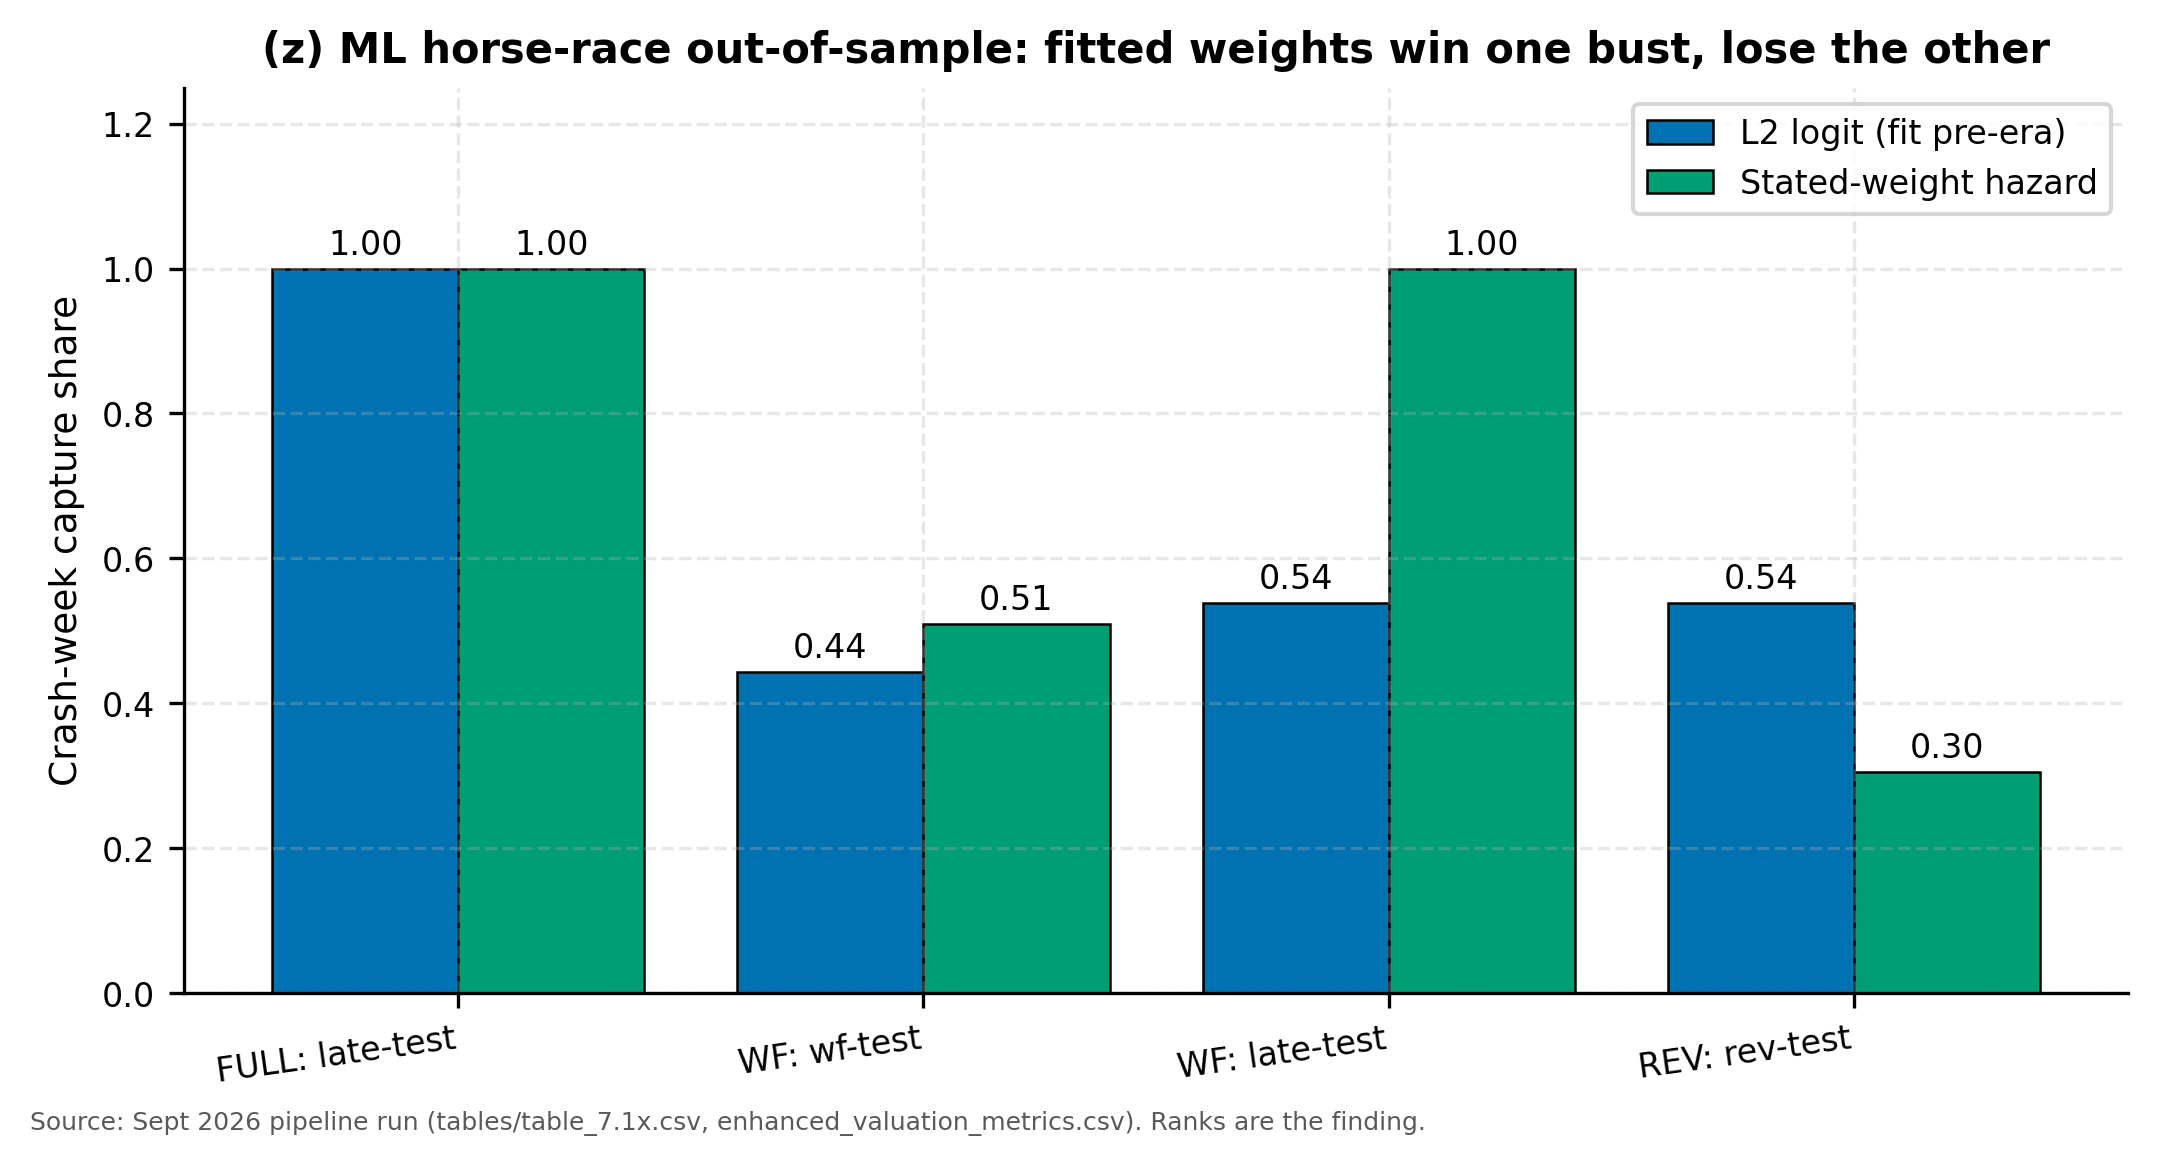
\includegraphics[width=\textwidth,height=0.82\textheight,keepaspectratio]{pred_ml_horserace.png}
\caption{ML horse-race out-of-sample crash capture: fitted L2 logit vs stated-weight hazard. The dot-com fit loses the GFC test; the GFC fit wins the dot-com test; the full fit ties the recent test. No weight vector wins everywhere --- bust shapes differ, so judgment-weighted gauges keep the job.}
    \label{fig:ml-horserace-oos}
\end{figure}

\begin{figure}[htbp]
\centering
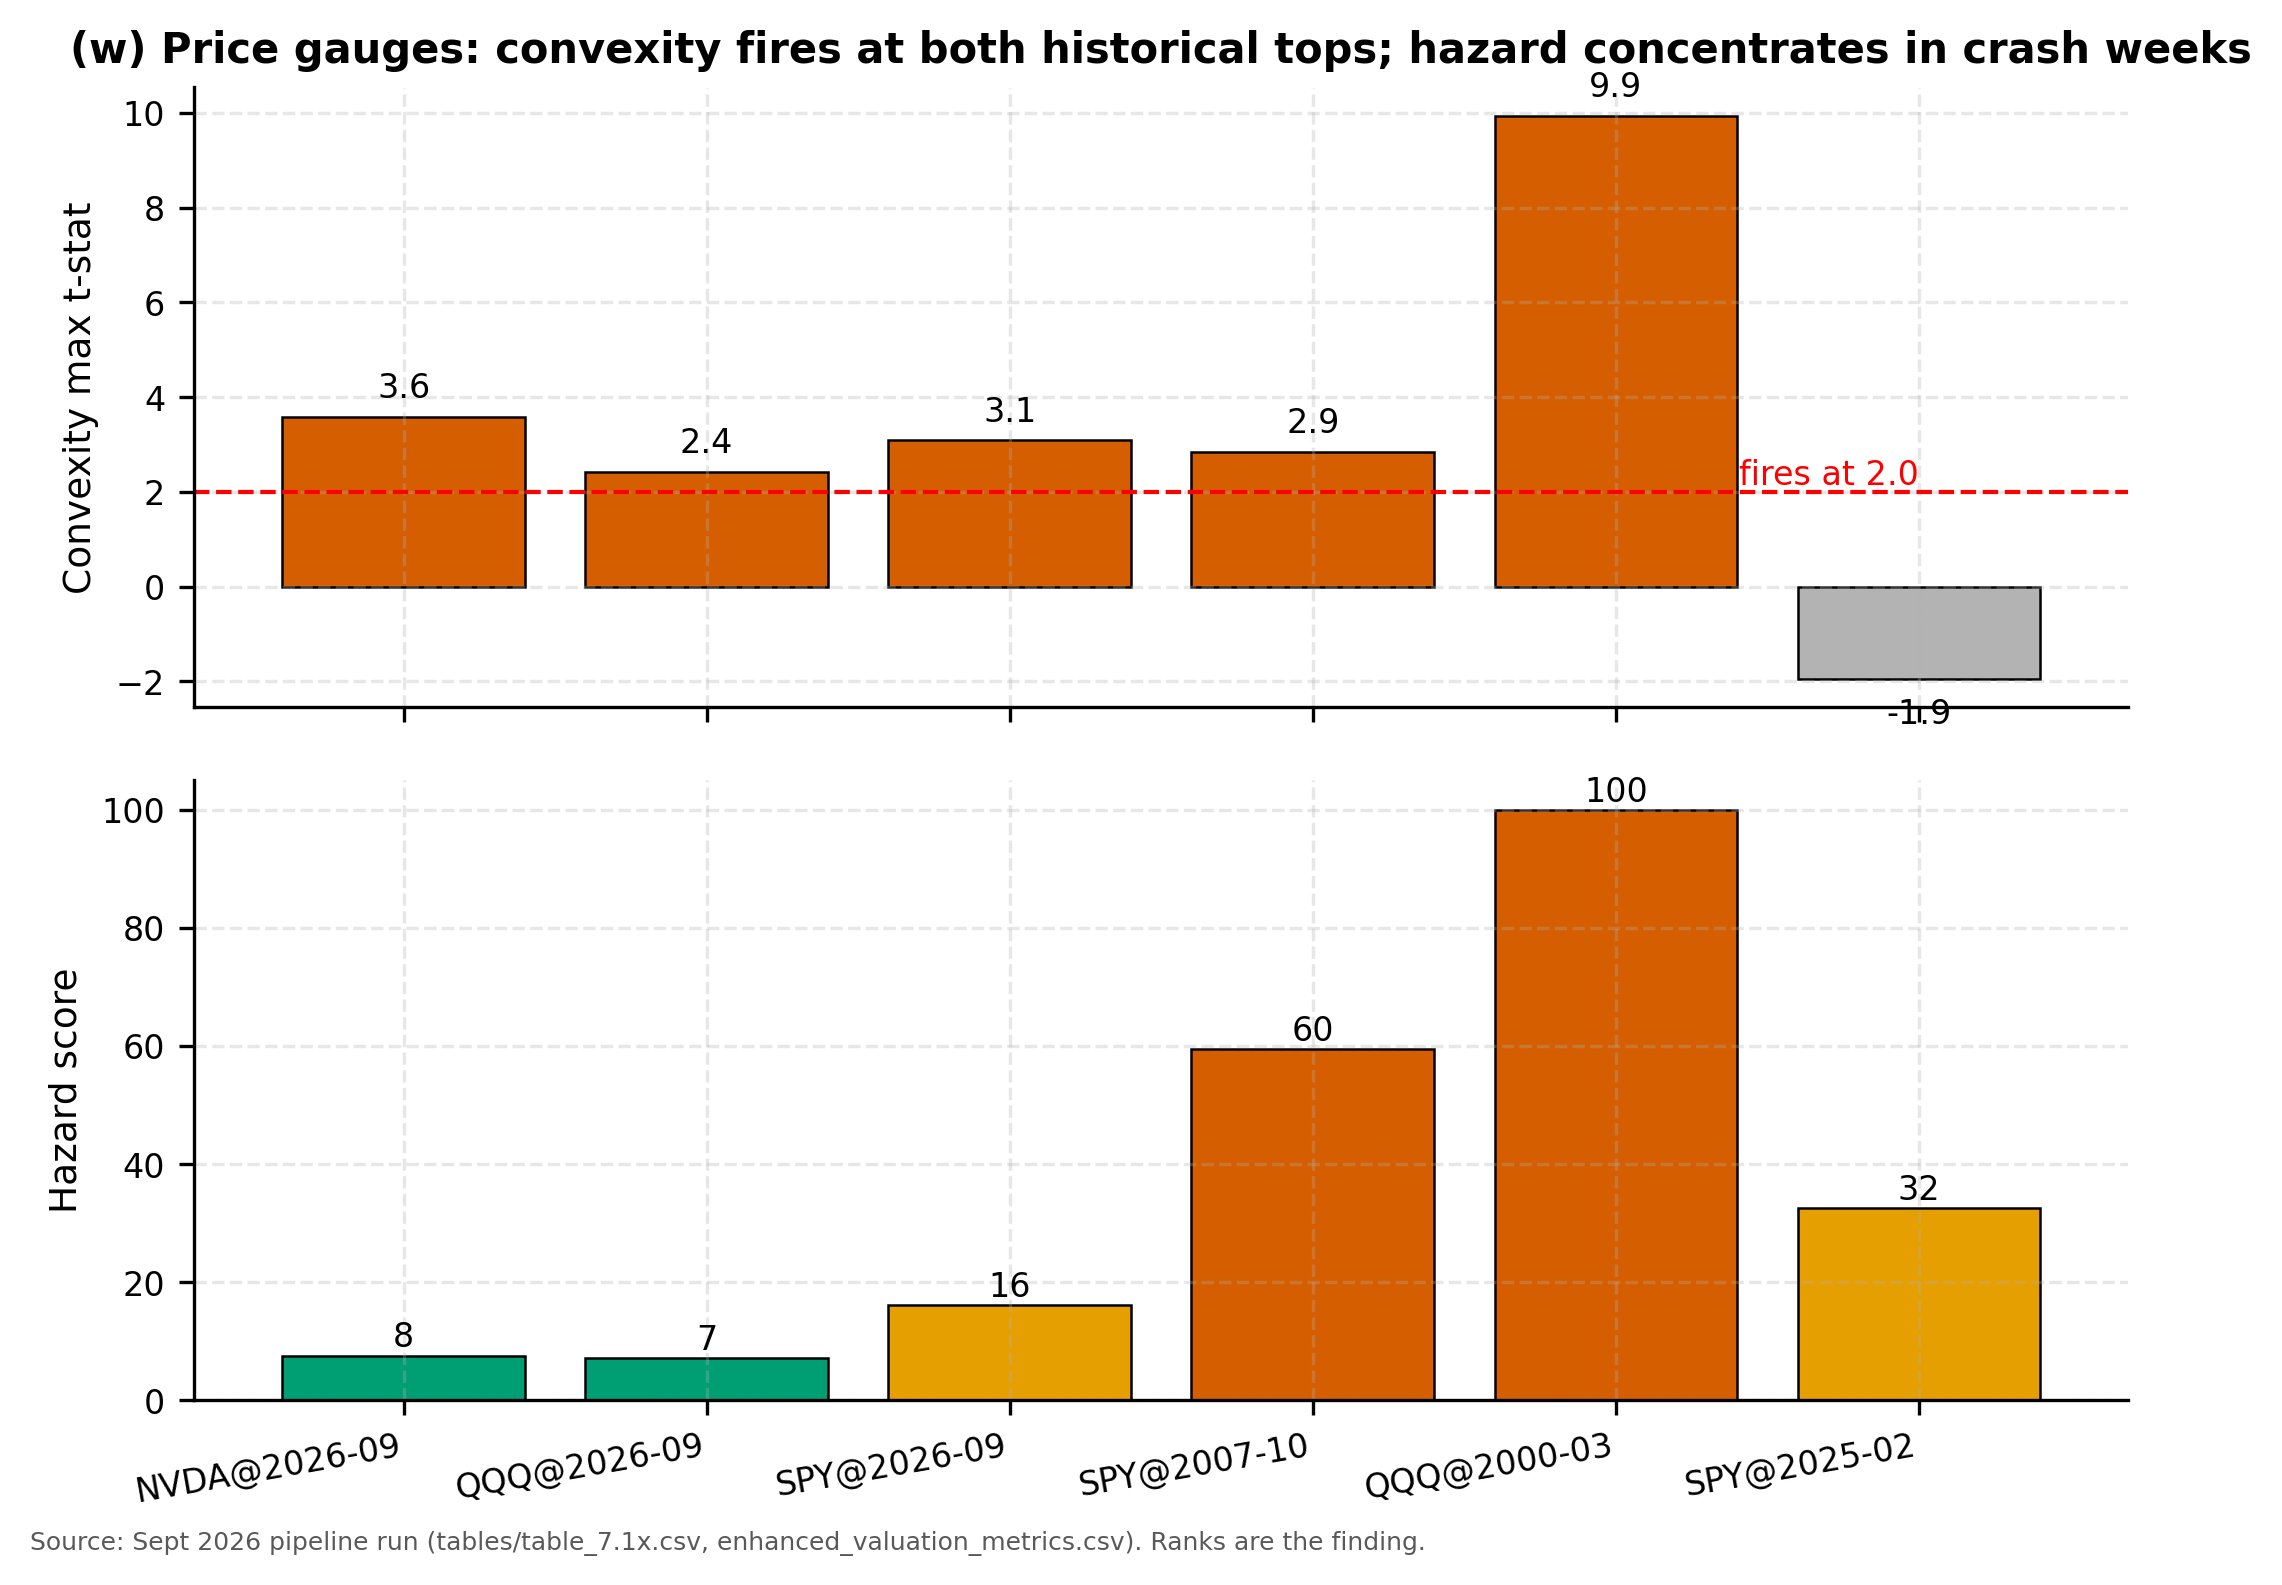
\includegraphics[width=\textwidth,height=0.82\textheight,keepaspectratio]{pred_gauge_backtest.png}
\caption{Price gauges across live names and frozen backtests. Top: convexity max $t$-statistic (fires at 2.0) --- both historical tops fire, February 2025 reads negative. Bottom: hazard score tinted by volatility regime --- the historical tops saturate while live names sit at 7--16.}
    \label{fig:price-gauges-backtest}
\end{figure}

\section{Scenario Analysis: Mild, Severe, and Conditional Activation}\label{sec:scenarios}
\emph{Mild} (capex trimmed, wealth wobbles): GDP cost $\sim$\$48.2B
(0.157\%) --- painful quarter, no recession print. \emph{Severe} (the
modeled case: 70\% of circular capital impaired, 30\% capex cut): GDP cost
$\sim$\$139.1B (0.452\%), concentrated upstream. \emph{Activation} (the
conditional \$60B lands \emph{before} any stress): the booked frame swells
toward \$735B, every burst number in this paper scales up roughly 9\%, and
the fire-sale channel gets more collateral to burn. If the \$500B facility
were ever drawn, it would nearly double the frame and move this analysis
from a sectoral call to a macroprudential one. The base prediction is
the severe case; activation before stress makes it worse, while early policy
response (disclosure plus caps, bought early) makes the mild case likelier.

\begin{table}[htbp]
\centering
\caption{Scenario ledger (\$B unless noted). Activation rows are proportional scalings (x735/675.4), not recomputed equilibria; DebtRank reverberation is modeled severe-only. Machine-readable: \texttt{pred\_A\_scenario\_ledger.csv}.}
    \label{tab:14-scenario-ledger-b-unless}
\begin{tabular}{lccccc}
\toprule
Scenario & Frame & Direct & 2nd round & GDP & GDP share \\
\midrule
Mild & 675.4 & 111.9 & n/a & 48.2 & 0.157\% \\
Severe (base) & 675.4 & 478.3 & 15.2 & 139.1 & 0.452\% \\
Activation-then-severe & 735.0 & 520.5 & 16.5 scaled & 151.4 & 0.492\% \\
\bottomrule
\end{tabular}
\end{table}

\section{Firm-Level Vulnerability Assessment}\label{sec:firms}
The screen's verdicts translate into a casualty order. \textbf{NVIDIA}
(\$5,280B, 31.7x) and \textbf{Broadcom} (\$1,500B, 35.7x) are the last to
fall: cash-covered multiples plus the top sustainability scores (78 and 76).
A demand break still cuts them first in dollars --- Hardware absorbs
\$239.4B --- but they have earnings to fall back on. \textbf{Microsoft}
(\$3,600B, 27.1x) and \textbf{Oracle} (\$480B, 28.5x) are screened Positive
on cash flow, with Oracle the live warning that leverage reprices even
healthy franchises: record CDS, lost rating cushion. \textbf{AMD} (\$746B,
89.2x) and \textbf{ServiceNow} (\$151B, 84.7x) are the two outright
Negatives --- multiples with no circularity cushion and no miss tolerance.
\textbf{Anthropic} (\$965B, earnings unattributed) is the single largest
unverified number in the stack: a walks-like-revenue \$65B run-rate against
a mark that assumes it compounds. \textbf{OpenAI} (\$852B, $\sim\!-35\%$
margins) burns to grow; its \$105B Ohio guarantee chain makes NVIDIA a
co-borrower in all but name. \textbf{CoreWeave} (\$70B, loss-making) is
the fire-sale prototype: homogeneous collateral, single-supplier dependence,
short-dated funding. \textbf{Databricks} (905x) and \textbf{xAI} (400x
revenue) are momentum marks awaiting earnings that may never arrive at the
assumed scale. \textbf{Intel} (\$110B, Neutral on an N/A multiple) matters as the
contrarian indicator: if the laggard rallies while leaders stall, the market
is pricing scarcity, not growth --- late-cycle behavior.

\emph{Who loses what.} Table~7.11's archetype totals split across the
23 screened companies on two stated bases: market-cap pro-rata and
deal-flow weight, where each company's attributed circular-deal flow comes
from the 19-row frame. NVIDIA midpoint \$198.3B (\$159.7B size basis,
\$236.9B deal basis) absorbs nearly all of Hardware's deal lens --- every
circular GPU flow runs through it. Anthropic midpoint \$41.7B and
OpenAI midpoint \$31.5B top the lab ledger; Microsoft Azure (\$36.4B) and AWS
(\$34.6B) top Cloud. The concentration flag is Lambda Labs: \$27.2B
midpoint on a \$5B mark, a capped 100\% haircut --- tiny neocloud, outsized
flow exposure. Google Cloud and Broadcom read \$0 on the deal basis (no
measured circular flow), an honest zero beside their size-basis shares.
Machine-readable: \texttt{pred\_H\_company\_losses.csv}.

\begin{figure}[htbp]
\centering
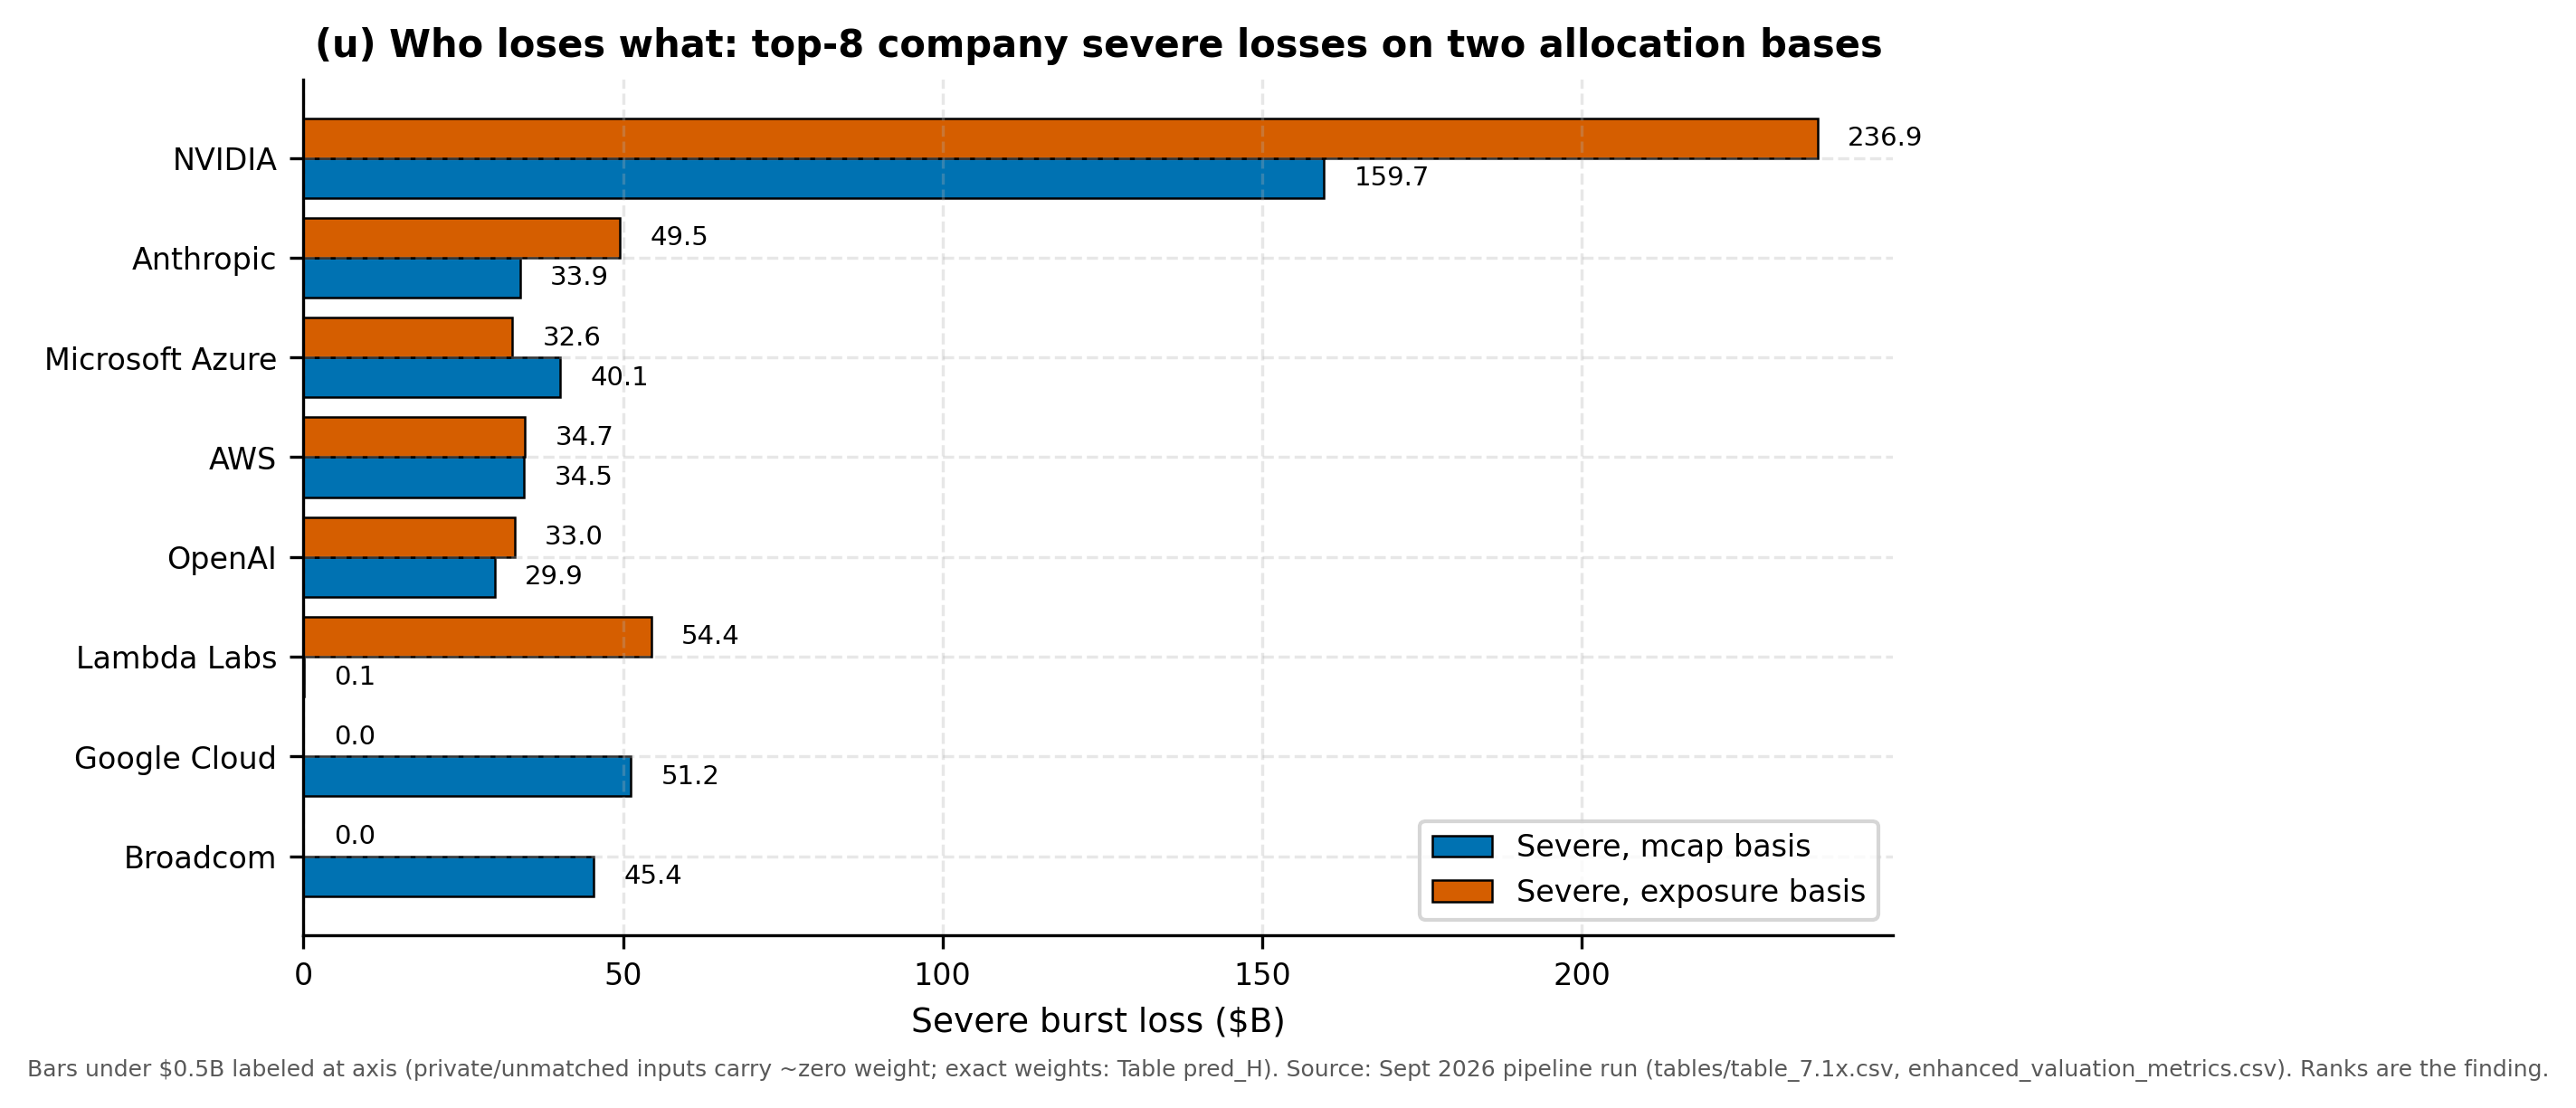
\includegraphics[width=\textwidth,height=0.82\textheight,keepaspectratio]{pred_company_losses.png}
\caption{Top-8 company severe losses on two allocation bases. Size basis follows market capitalization; deal basis follows attributed circular-deal flow. NVIDIA dominates both; Lambda Labs' deal bar against its sliver of a size bar is the stack's concentration risk in one picture.}
    \label{fig:company-severe-losses}
\end{figure}

\emph{Expected losses: probability-weighted.} Blending the two severities by
each archetype's formation probability as the severe-burst probability
inside the window --- an upper-bound convention, stated in the ledger, not a
measured burst frequency --- gives the expected-loss ranking that answers
who loses how much: NVIDIA expected \$164.3B, Anthropic expected \$36.7B
and OpenAI expected \$27.7B lead, followed by Microsoft Azure (\$22.6B) and
AWS (\$21.6B). The driver column says \emph{why} each number is what it is:
the top three are deal-flow-driven (their circular-deal weight exceeds their
size weight), while Microsoft Azure and Broadcom (\$18.8B) are
size-driven. Lambda Labs' expected \$16.9B exceeds its \$5B mark severalfold
(haircut capped at wipeout) --- the concentration flag survives
probability-weighting. Machine-readable:
\texttt{pred\_K\_expected\_losses.csv}.

\begin{figure}[htbp]
\centering
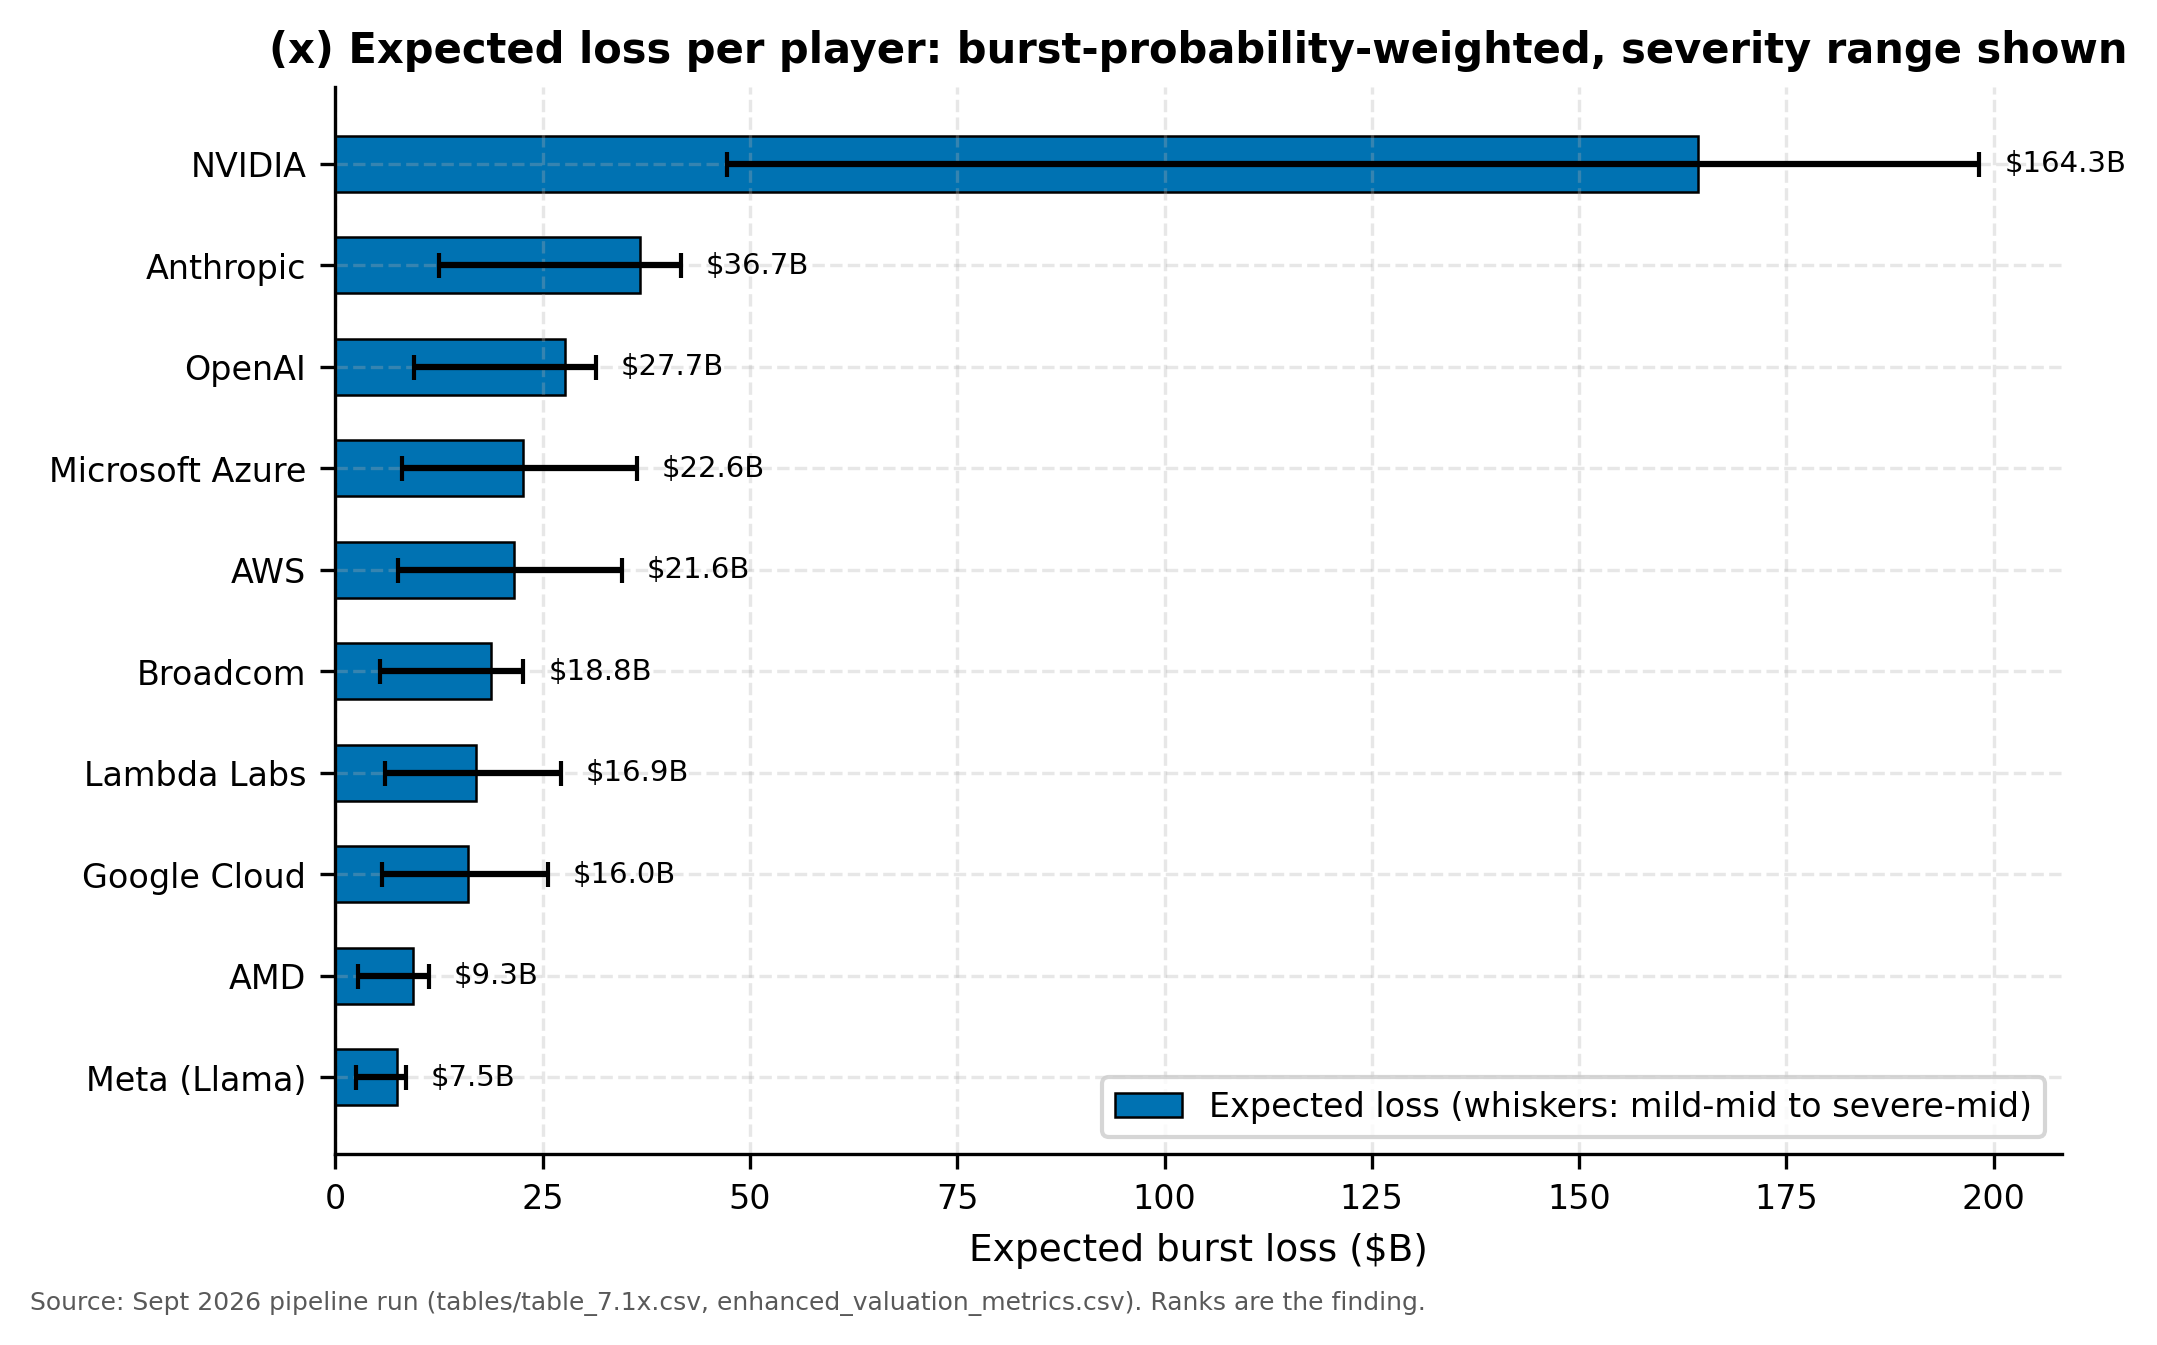
\includegraphics[width=\textwidth,height=0.82\textheight,keepaspectratio]{pred_expected_losses.png}
\caption{Top-10 expected burst losses with severity ranges. Bars blend severe and mild by each archetype's formation probability; whiskers span mild-mid to severe-mid. NVIDIA's bar is a deal-flow story; Azure's and Broadcom's are size stories.}
    \label{fig:expected-losses-top10}
\end{figure}

\emph{How the flags are built.} The screen flags 4 Positive (NVIDIA at 31.7x trailing, Broadcom at 35.7x, Microsoft at 27.1x, Oracle at 28.5x), 2
Negative (AMD at 89.2x, ServiceNow at 84.7x) and 17 Neutral on trailing
P/E and EV/Revenue multiples. Diversified hyperscalers enter at parent
market capitalization because segment revenue against a parent cap would
fabricate multiples; attributed-revenue units (Google TPU, Meta Llama) are
capped at Neutral regardless of arithmetic, since attribution is not
audit-grade. The forward multiple is trailing P/E scaled by one minus the
revenue-growth rate (Broadcom: $35.7\times(1-0.80)\approx 7.1\times$),
clamped to a maximum 99\% haircut so hyper-growth can never flip the sign
--- a first-order, growth-rewarding shorthand rather than a
forecasted-earnings construction. Loss-makers and unattributed-margin
frontier labs show N/A trailing multiples and rate Neutral rather than
Negative: the discipline is to distinguish unprofitability-by-investment
from overvaluation-by-multiple. These are triage screen flags, not
investment ratings: no Buy/Sell/Hold recommendation is issued.

\emph{What incumbents should do.} The core game's Pareto cell exceeds the
Nash cell by \$58.6B: there is a purchasable surplus from coordinated
openness, and firms that pre-commit to portability standards capture
first-mover goodwill while blunting the antitrust case against them. For
labs, the formation ranking is a funding warning: diversifying compute
supply and converting conditional tranches into committed, covenant-light
capacity reduces both financing risk and the appearance of circularity that
disclosure rules would in any case reveal. For neoclouds and GPU-debt
vehicles, the message is concentration arithmetic: stagger maturities,
diversify silicon, and publish recovery rates --- the cheapest
self-insurance available.

\section{Portfolio Implications and Risk Management}\label{sec:portfolio}
Own the cash-generative infrastructure core; underweight the densest
round-trippers; hedge the uncovered multiples; let funding rounds and
chip-collateral spreads move the odds.

\begin{figure}[htbp]
\centering
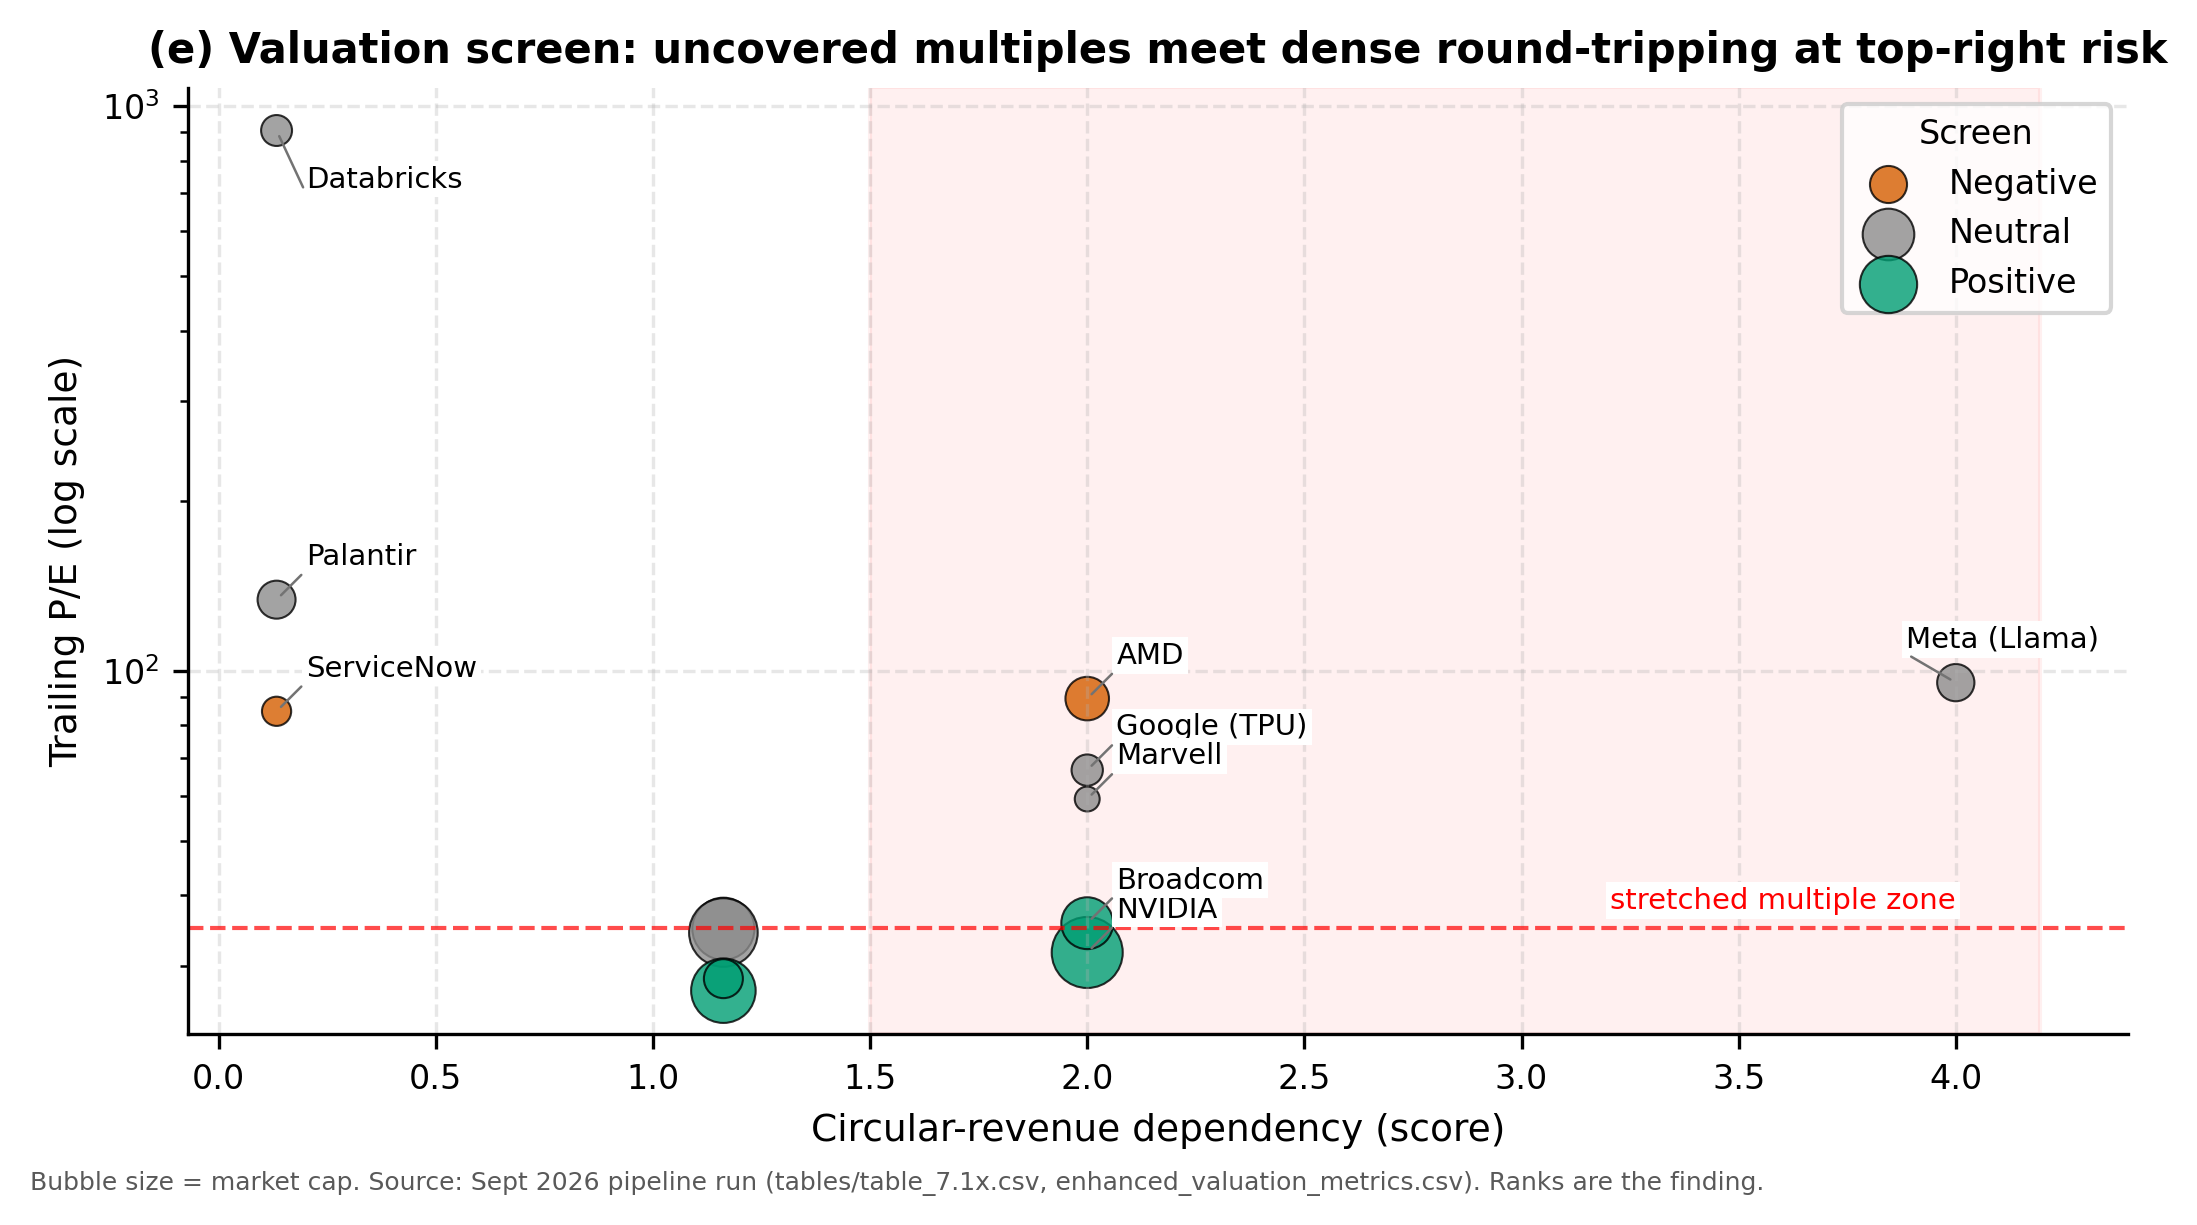
\includegraphics[width=\textwidth,height=0.82\textheight,keepaspectratio]{pred_valuation_scatter.png}
\caption{Trailing P/E (log scale) vs.\ circular-revenue dependency, sized by market cap, colored by screen flag. The shaded danger zone (stretched multiple \emph{and} dense round-tripping) holds four names, and only one carries a Negative screen flag: AMD (89x). Google TPU (67x), Marvell (59x), and Meta (95x) share the region as Neutrals. The cloud majors cluster on the stretched-multiple line; Databricks (905x) plots top-left --- extreme multiple without round-tripping; xAI (400x EV/Rev) carries no trailing P/E and does not plot.}
    \label{fig:23-trailing-pe-log-scale}
\end{figure}

\begin{table}[htbp]
\centering
\caption{Valuation screen: flagged names only (4 Positive, 2 Negative, 5 flagged Neutral). Full 23-company ledger: \texttt{pred\_C\_valuation\_watchlist.csv}.}
    \label{tab:15-valuation-screen-flagged-names}
\begin{tabular}{llccl}
\toprule
Company & Arch. & Mkt cap & Multiple & Screen \\
\midrule
NVIDIA & HW & 5,280 & 31.7x P/E & Positive \\
Broadcom & HW & 1,500 & 35.7x P/E & Positive \\
Microsoft & Cloud & 3,600 & 27.1x P/E & Positive \\
Oracle & Cloud & 480 & 28.5x P/E & Positive \\
AMD & HW & 746 & 89.2x P/E & Negative \\
ServiceNow & Wrap & 151 & 84.7x P/E & Negative \\
Anthropic & FM & 965 & n/a & Neutral (flagged) \\
OpenAI & FM & 852 & neg. margin & Neutral (flagged) \\
xAI & FM & 200 & 400x EV/Rev & Neutral (flagged) \\
Databricks & Wrap & 190 & 905x P/E & Neutral (flagged) \\
CoreWeave & Cloud & 70 & loss-making & Neutral (fire-sale proto.) \\
\bottomrule
\end{tabular}
\end{table}

Pair-trade logic follows the burst order: positions long one side of a
Hardware--Cloud pair and short the other collect the spread only in mild
states, because a severe burst impairs both sides of the largest contracts
at once. Size positions off ranks (which survive), never off point GDP
costs (which expire with the vintage).

\begin{figure}[htbp]
\centering
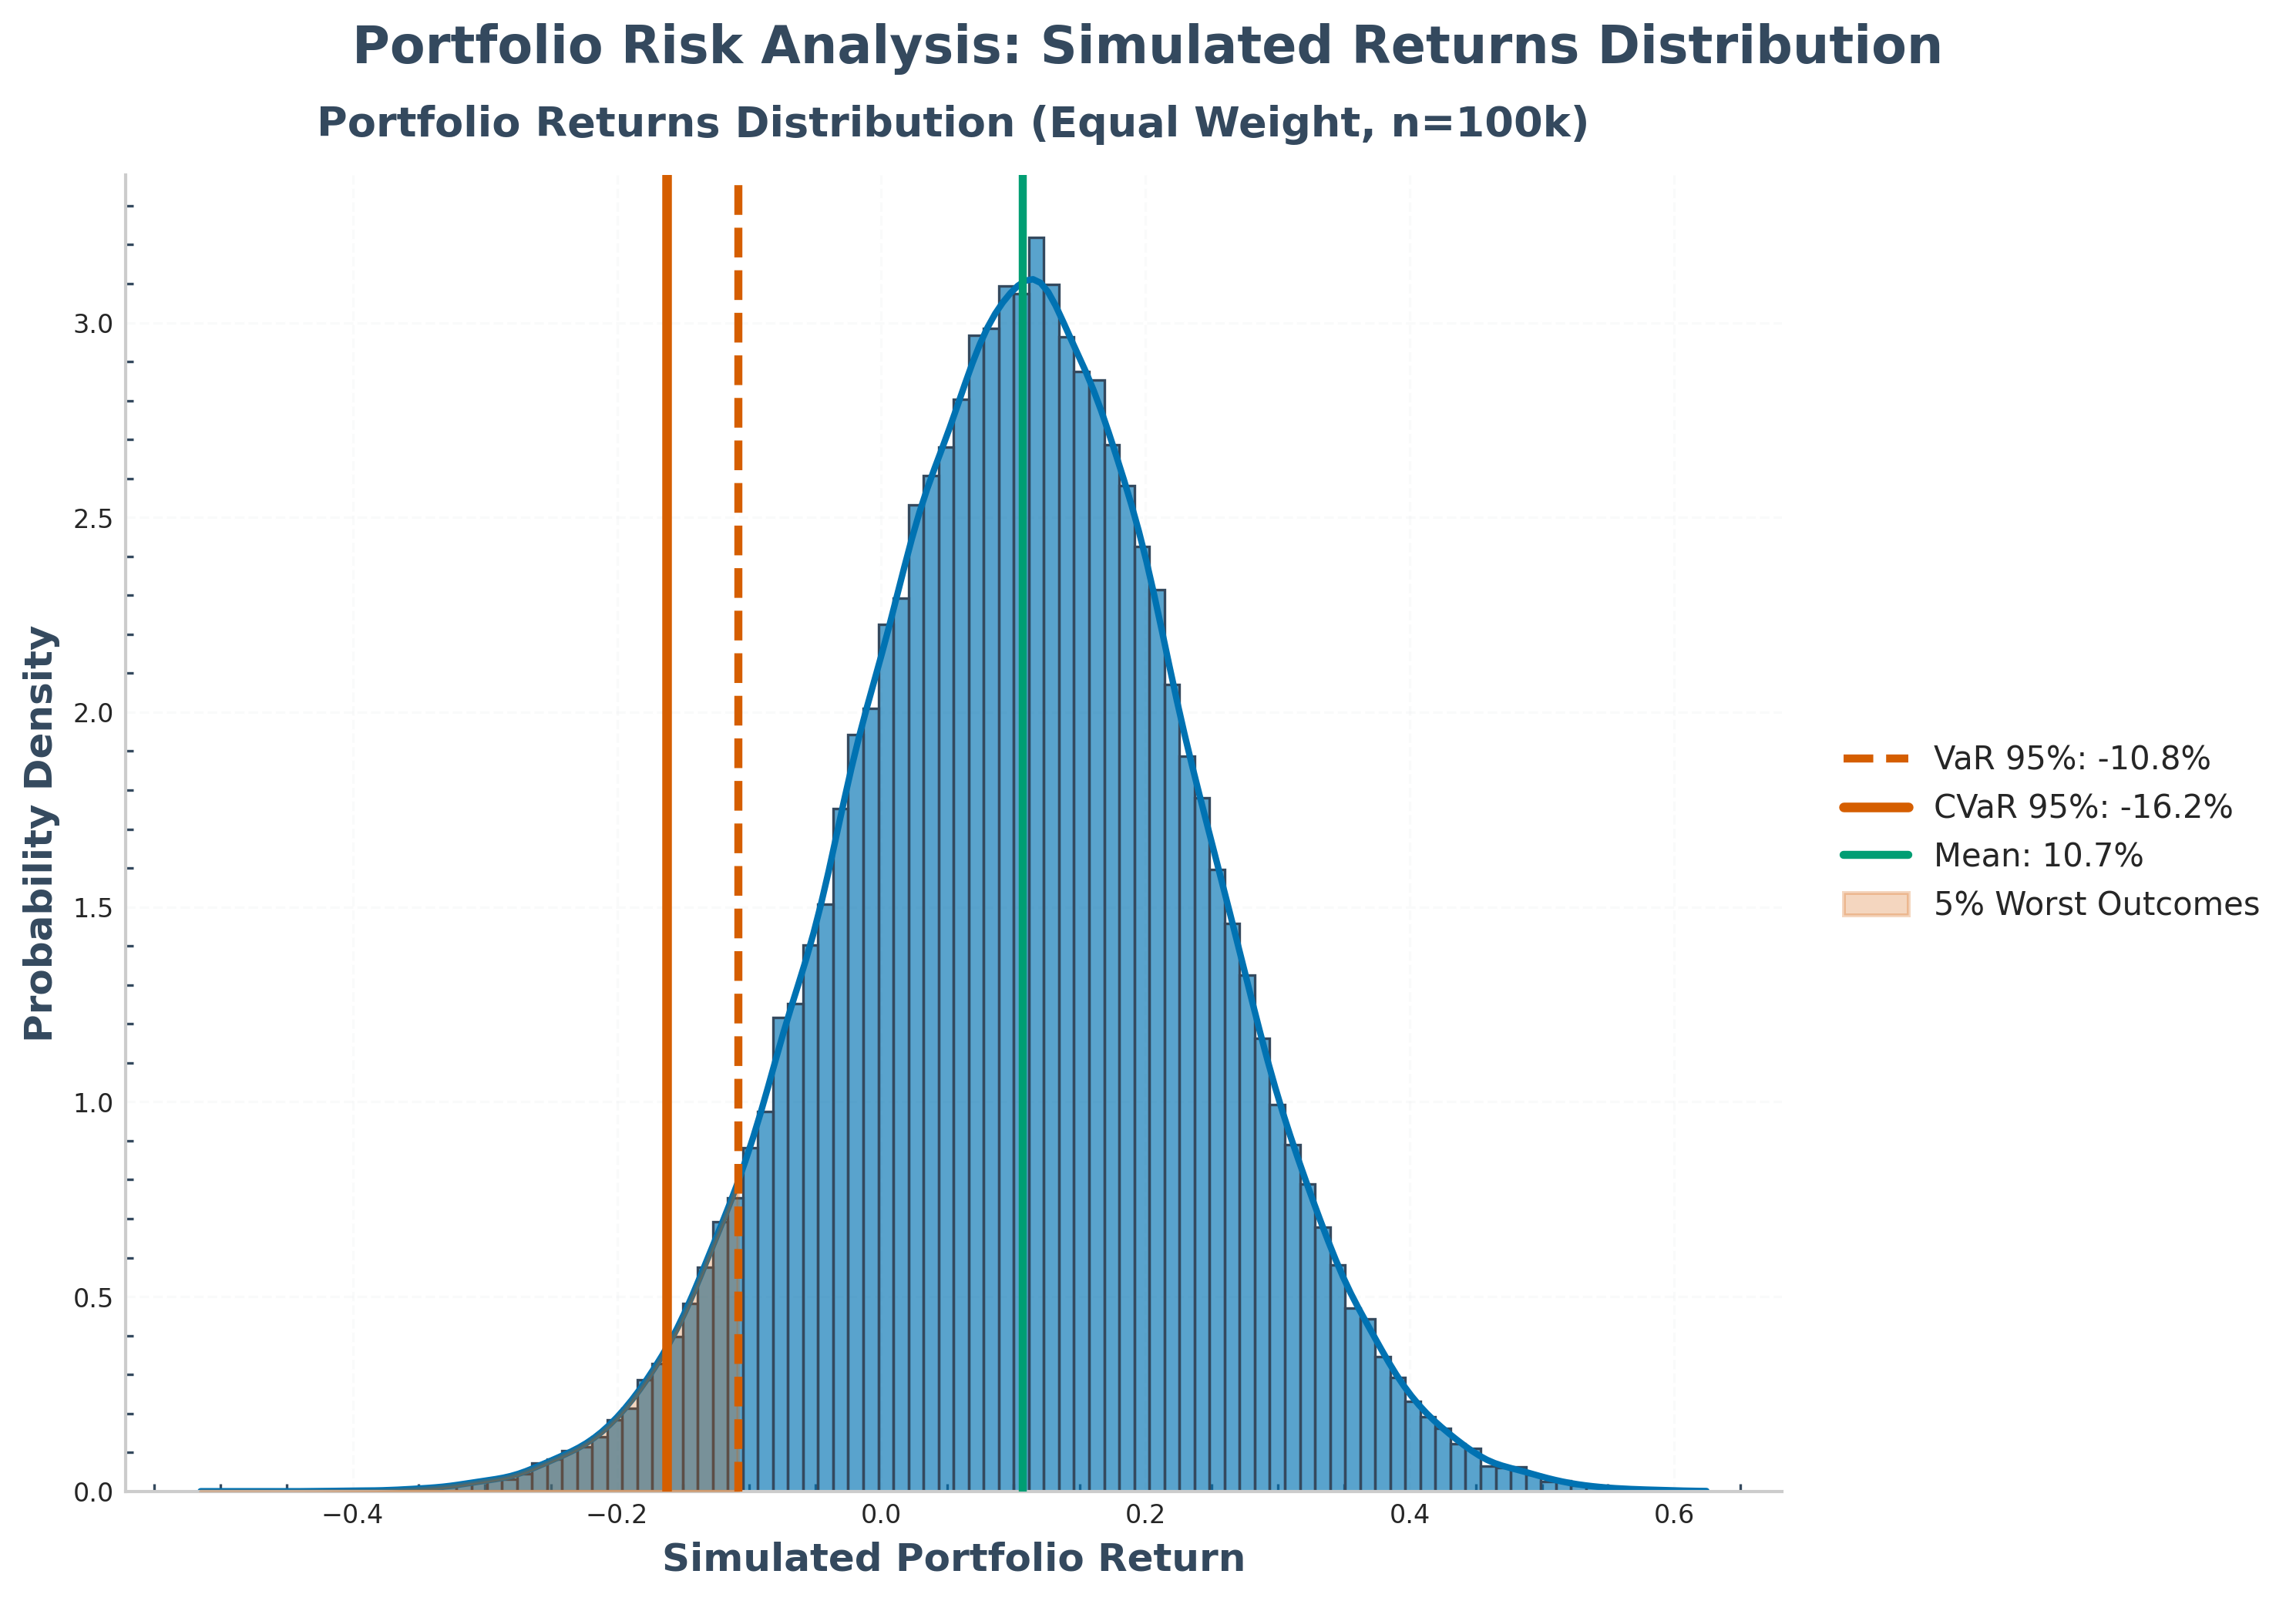
\includegraphics[width=0.85\textwidth,height=0.82\textheight,keepaspectratio]{figure_15.png}
\caption{Diversification arithmetic (Table~A.2): the stack portfolio earns 10.7\% mean return at 13.0\% volatility (Sharpe 0.82), but the left tail is a burst tail --- 95\% VaR of $-10.8\%$, conditional tail (CVaR) of $-16.2\%$. The mean compensates holders for volatility, not for the correlated unwind; hedge the tail, not the mean.}
    \label{fig:05-diversification-arithmetic-tablea2-the}
\end{figure}

\emph{For banks, lenders, and risk functions.} Collateral haircuts
calibrated on generic equipment schedules understate wrong-way risk:
homogeneous, supplier-guaranteed GPU collateral correlates exactly when it
must be sold. Lenders should haircut GPU collateral against a
circularity-adjusted recovery rate and covenant single-name exposure to
leveraged secondary nodes (Oracle, CoreWeave, and neocloud vehicles are
named by both the cascade analysis and the burst ranking). The 215bp
Oracle CDS print and BBB- downgrade show credit markets already price part
of this; this paper's contribution is the stack-wide incidence map that
tells a risk committee \emph{which} names reprice next. Risk functions can
operationalize the portable rule immediately: per \$100B of destroyed AI
value, book \$4.0B of wealth-channel GDP drag and add the domestic
capex-cut share, and scale by local capex intensity elsewhere. Scenario
design should include a multi-stage cascade structure (macro shock meeting
stretched credit) rather than a single-factor tech selloff, and recovery
planning should pre-negotiate data-center collateral conversion terms.

\section{Policy Sequencing by Benefit--Cost Ratio}\label{sec:policy}
Every remedy studied returns more than it costs --- but doing everything at
once is worth less than the sum of its parts (combined DWL package \$214.2B
against \$418.9B of standalone gains: synergy ratio 0.547). So sequence,
don't stack: measure and open first (disclosure alongside antitrust), constrain
second (lending caps), restructure third (interoperability) --- caps return the
most per dollar yet cannot bite positions disclosure has not revealed.

\begin{figure}[htbp]
\centering
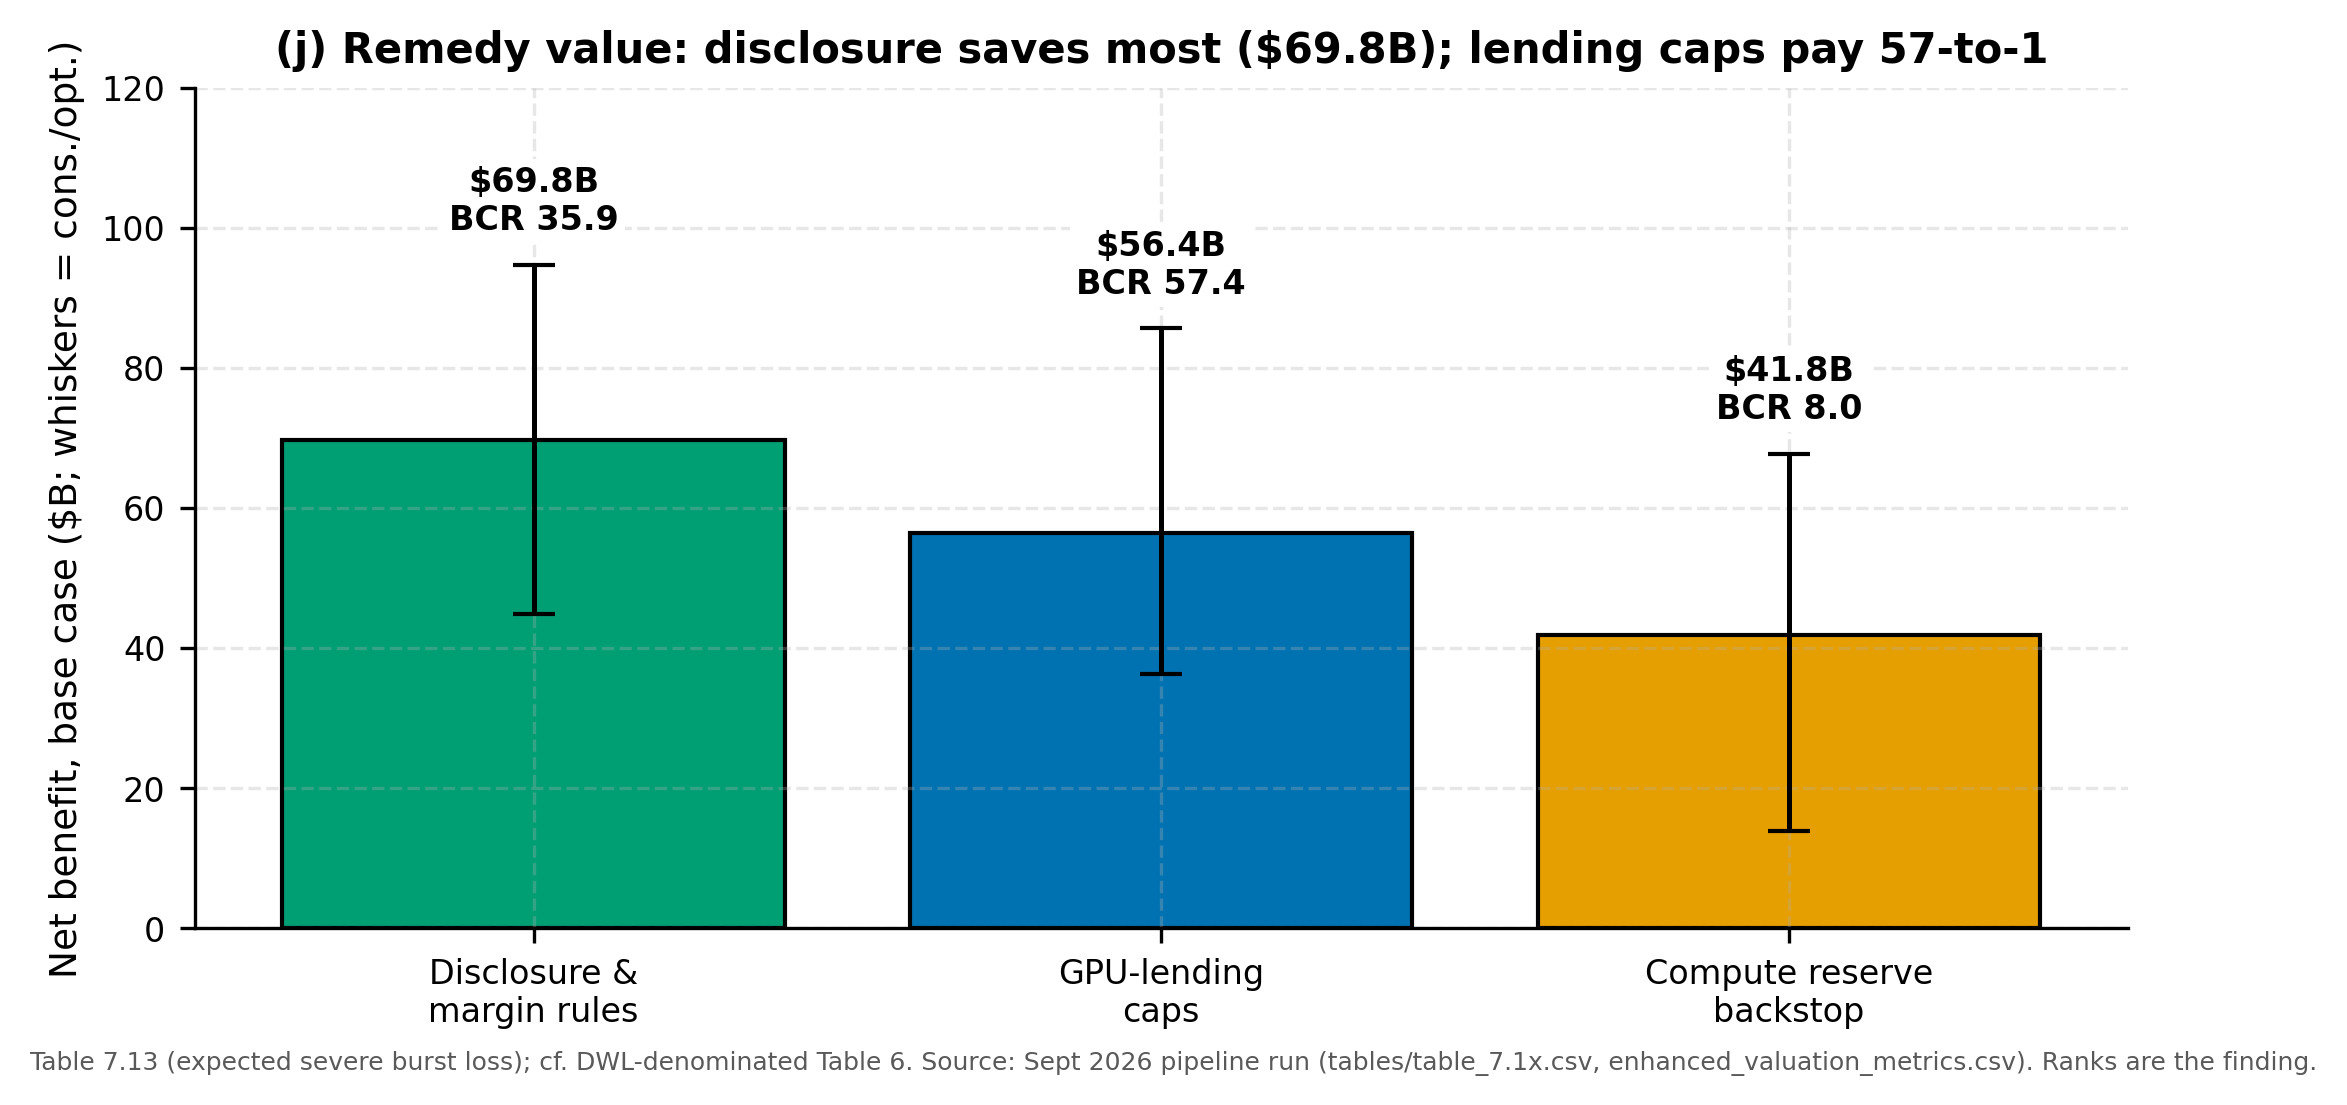
\includegraphics[width=\textwidth,height=0.82\textheight,keepaspectratio]{pred_bubble_policy_bcr.png}
\caption{Burst-denominated remedy value (Table~7.13): net benefit in the base case with conservative/optimistic whiskers. GPU-lending caps return \$56.4B on \$1B (BCR 57.4); disclosure returns \$69.8B on \$2B (BCR 35.9). Denominated in expected severe burst loss rather than deadweight loss, so the numbers below complement --- rather than duplicate --- the DWL-based table that follows.}
    \label{fig:24-burstdenominated-remedy-value-table713}
\end{figure}

\begin{table}[htbp]
\centering
\caption{Burst-denominated remedies (Table~7.13): ordered by value per dollar.}
    \label{tab:16a-burstdenominated-remedies-table713}
\begin{tabular}{lccc}
\toprule
Remedy & BCR & Net (\$B) & Cost (\$B) \\
\midrule
GPU-lending caps & 57.4 & 56.4 & 1.0 \\
Deal disclosure & 35.9 & 69.8 & 2.0 \\
Combined package & 15.9 & 134.5 & 9.0 \\
Strategic reserve & 8.0 & 41.8 & 6.0 \\
\bottomrule
\end{tabular}
\end{table}

\begin{table}[htbp]
\centering
\caption{Deadweight-loss-denominated remedies (Table~6): ordered by value per dollar.}
    \label{tab:16b-deadweightlossdenominated-remedies-table}
\begin{tabular}{lccc}
\toprule
Remedy & BCR & Net (\$B) & Cost (\$B) \\
\midrule
Antitrust enforcement & 52.1 & 102.2 & 2.0 \\
API interoperability & 29.2 & 140.9 & 5.0 \\
Data sharing mandate & 25.0 & 72.0 & 3.0 \\
Innovation subsidies & 11.7 & 85.8 & 8.0 \\
\midrule
Combined intervention & 15.3 & 214.2 & 15.0 \\
\bottomrule
\end{tabular}
\end{table}

Table~\ref{tab:policy-summary} states the paper's policy contribution in one
place: burst-denominated tools and DWL-denominated tools attack different
margins, so the two rankings complement rather than compete --- sequence
measurement and leverage control first, market-structure repair second.

\begin{table}[htbp]
\centering
\caption{Optimal policy sequencing across welfare and stability metrics.}
\label{tab:policy-summary}
\small
\begin{tabular}{lcccc}
\toprule
Policy Instrument & Primary Target & BCR (Burst) & BCR (DWL) & Regulatory Authority \\
\midrule
\textbf{1. Deal disclosure} & Information asymmetry & 35.9 & -- & SEC / FTC / DOJ \\
\textbf{2. GPU-lending caps} & Stack leverage & 57.4 & -- & Fed / OCC / BIS \\
\textbf{3. Antitrust enforcement} & Market-power markups & -- & 52.1 & DOJ / FTC / DG COMP \\
\textbf{4. API interoperability} & Switching costs / lock-in & -- & 29.2 & FTC / EU DMA \\
\bottomrule
\end{tabular}
\end{table}

\begin{figure}[htbp]
\centering
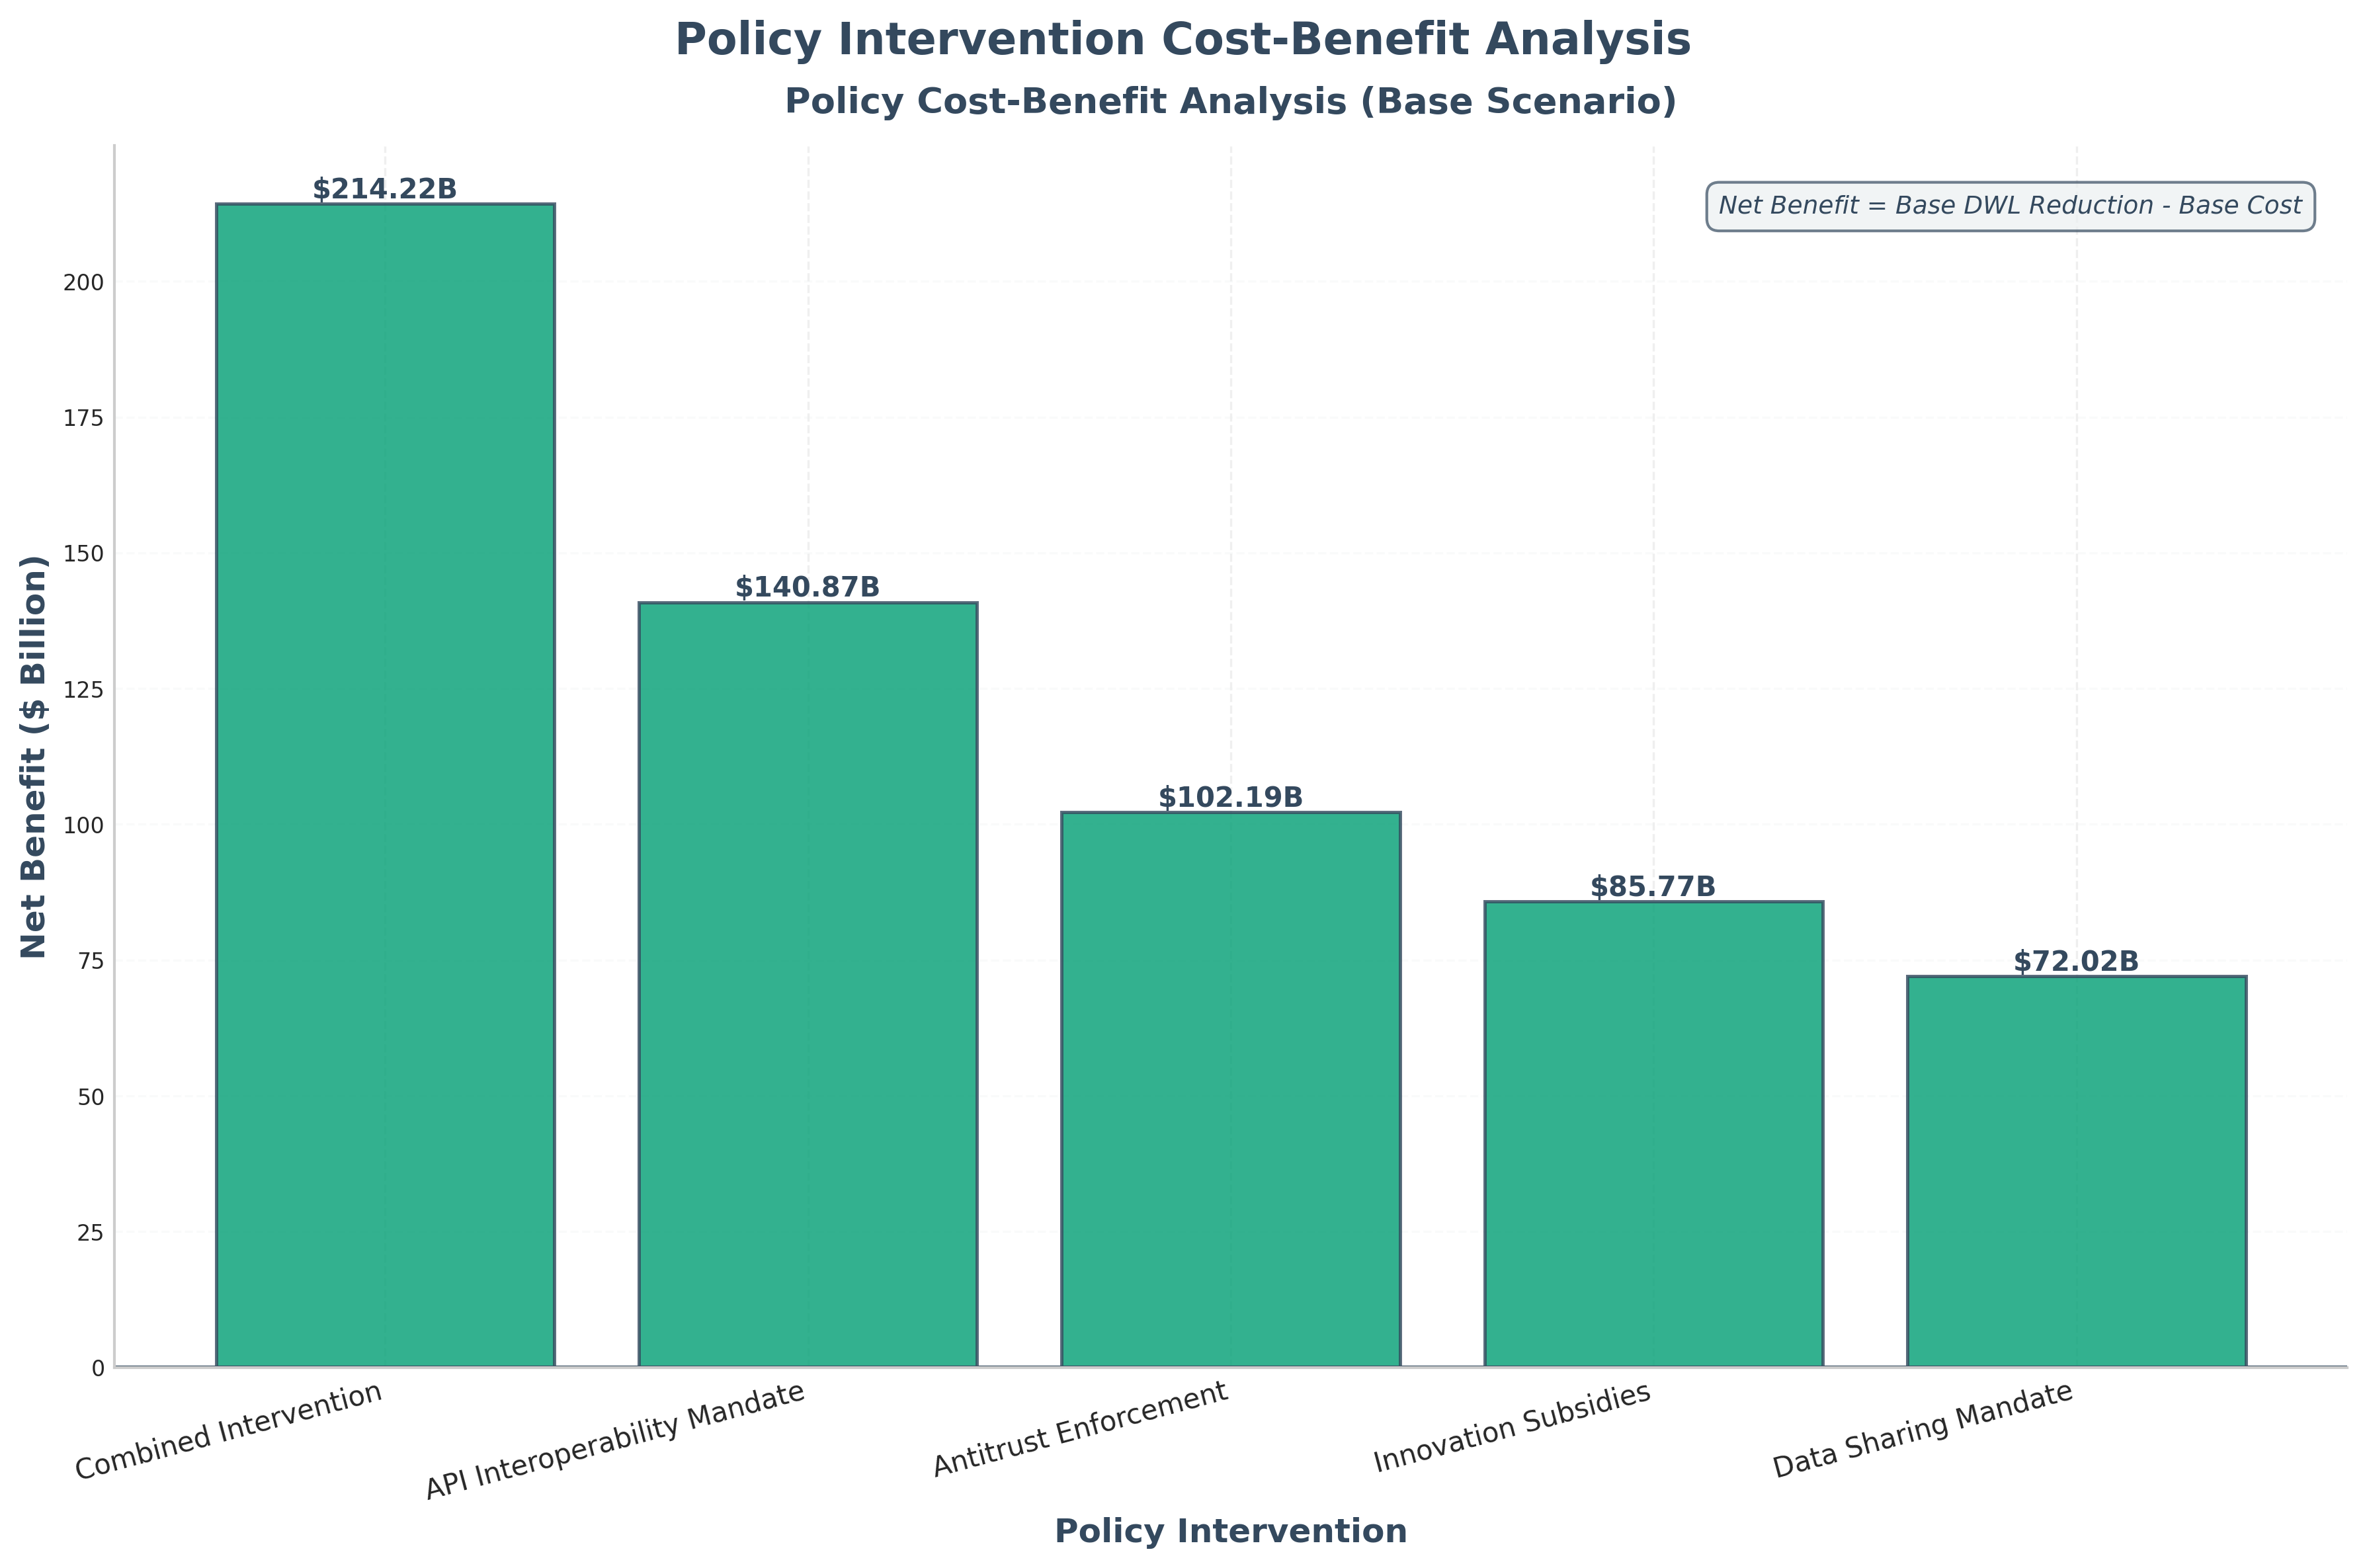
\includegraphics[width=0.9\textwidth,height=0.82\textheight,keepaspectratio]{figure_12.png}
\caption{Net benefit by intervention (\$B). The combined package exceeds any standalone tool, yet trails the sum of its parts --- the quantitative case for sequencing.}
    \label{fig:25-net-benefit-by-intervention}
\end{figure}

\begin{figure}[htbp]
\centering
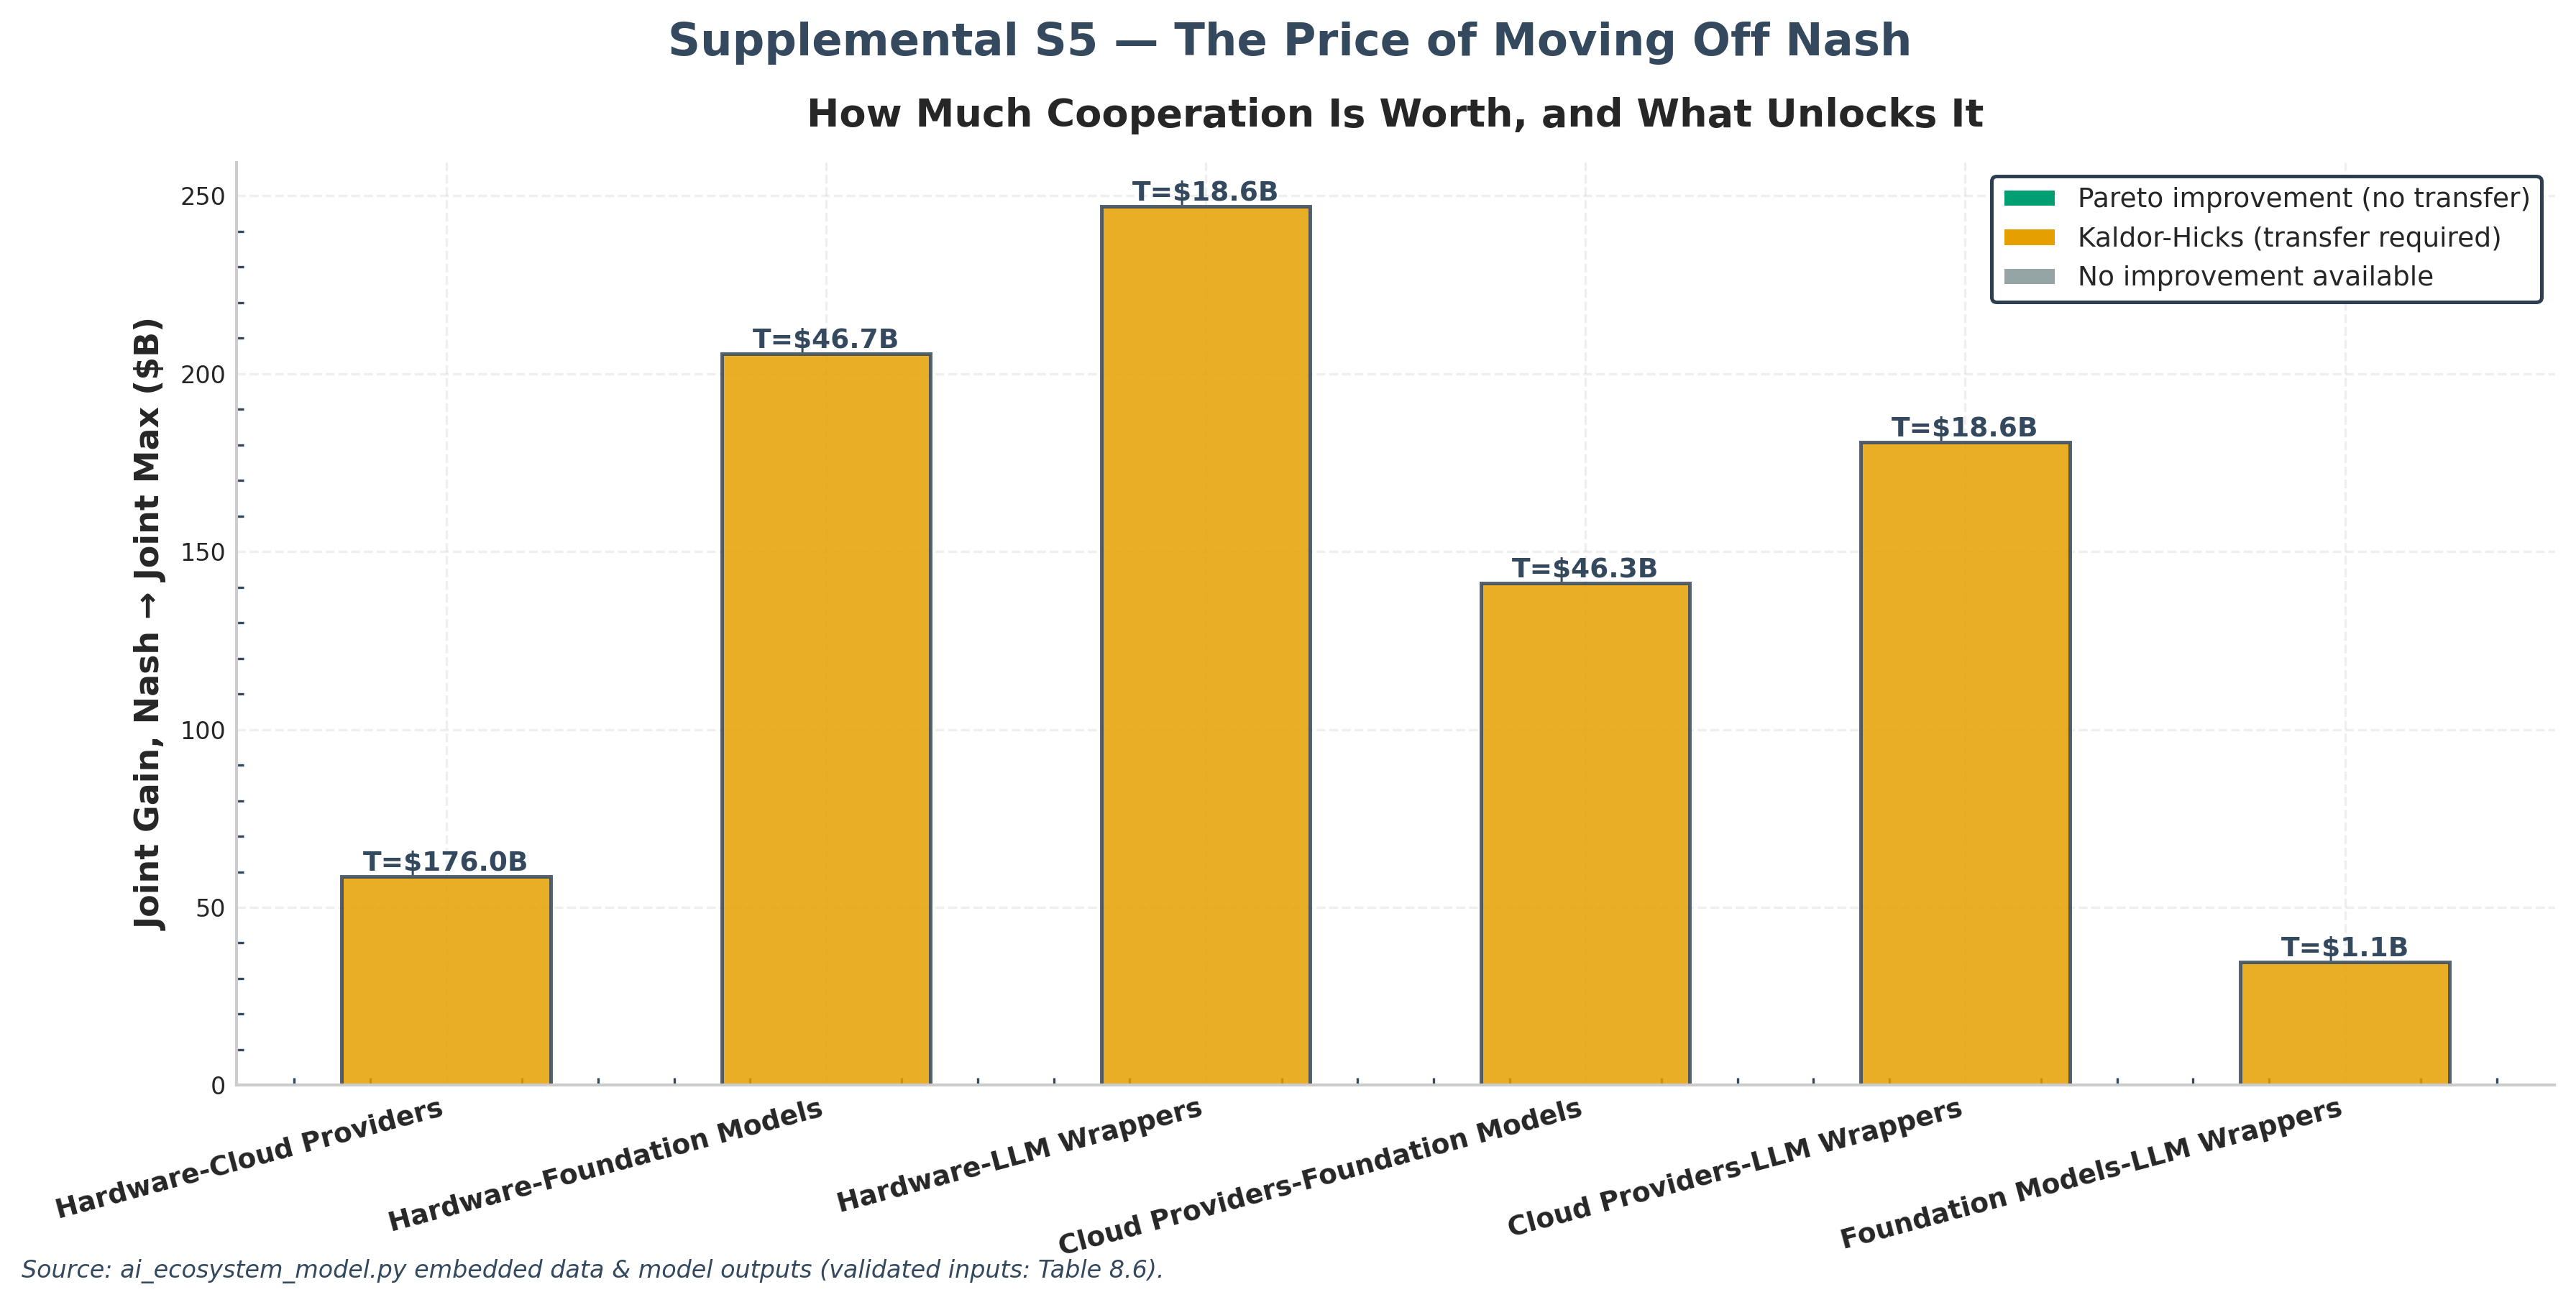
\includegraphics[width=\textwidth,height=0.82\textheight,keepaspectratio]{supplemental/s5_joint_gains_transfers.png}
\caption{Joint gains by relationship with the compensating transfers that unlock them. Every transition needs a payment; none is free --- which is why the prediction expects the stuck cells to persist until policy or crisis pays the transfer.}
    \label{fig:06-joint-gains-by-relationship}
\end{figure}

Break-even conditions and what the ratios omit are documented in the Online Appendix; the remedy ranking above is the result.
\section{Validation Tests}\label{sec:validation}
Three numbered tests retire the registry --- the same numbering the
registry's last column points to. \textbf{Test 1:} frontier labs converting
private marks into committed, profitable revenue at current scale (retires
P1 and P5). \textbf{Test 2:} conditional tranches activating on schedule
through a full cycle with no spread widening (retires P1). \textbf{Test 3:}
a demand break that spares Hardware --- the burst ranking flipping on
re-estimated exposures (retires P2, the paper's firmest claim). The
pipeline's 364 automated checks turn each into a failing gate, so the
call updates mechanically with new data: when a test trips, the
corresponding registry likelihood goes to near zero by construction, not by
reargument.

\section{Conclusion}
The central result of this paper is an incidence ranking with measured
foundations: \$675.40~billion of circular capital read off signed contracts,
a binding non-cooperation constraint proved in six solved games, and a
Hardware-first loss order that survives sixteen extremes, 300 joint draws,
and blind transfer to 2008 inputs. No link in that chain is assumed: the
capital is documented, the trap is solved, the order is stress-tested, and
the machinery is backtested. Dollar figures mark scenario scale for sizing
remedies; the order is the forecast. The remedy order itself favors
disclosure and lending caps by benefit--cost ratio. Three observables would
retire the call (Section~\ref{sec:validation}); until one fires, the
monitoring order in Section~\ref{sec:triggers} and the positioning rules in
Section~\ref{sec:portfolio} are the operational edge of the analysis.

Three broader lessons close the argument. First, \emph{structure dominates
sentiment}: once financing is round-tripped, contracts --- not narratives
about exuberance --- decide where losses land. The burst ranking therefore
differs from the formation ranking, and both are needed. Second,
\emph{disclosure is the cheapest stabilizer}: the highest burst-mitigation
BCRs reward revealing structure (35.9) and capping the leverage it invites
(57.4). Third, \emph{ranks travel while levels expire}: every number in
this paper will age with funding rounds and prices, but the orderings ---
the burst order, the remedy order, the loss-source order --- are built to
survive re-calibration. Technology can succeed while assets disappoint;
mapping the circle shows where. What remains is to decide, before the next
funding round redraws it, which edge to cut first.


\section*{Data and Code Availability}
\addcontentsline{toc}{section}{Data and Code Availability}
All code, tables, and figures are generated by a single Python pipeline.
To preserve double-blind review, the repository link is withheld from this
submission version; an anonymized replication archive will be provided upon
acceptance. Running \texttt{python3 run\_pipeline.py} from the repository
root regenerates every
numbered table and figure in order (model, technical report, dashboard,
tests, retirement exposure, article PDF, prediction exhibits, backtests, and
comparisons), gated by a 364-test suite that must pass before the article
typesets. Requirements are Python 3.12 with \texttt{numpy}, \texttt{pandas},
\texttt{matplotlib}, \texttt{openpyxl}, \texttt{python-docx},
and \texttt{beautifulsoup4} (\texttt{coverage} only for the
coverage report), plus a \texttt{pdflatex} distribution for the article;
each stage also runs standalone (see the repository README for per-stage
commands and runtimes). Random draws are seeded (global seed 42; joint
robustness check seed 7) for exact reproducibility. The only live network
call is an SEC EDGAR revenue fetch with a vendored offline fallback, so
builds are deterministic without network access; price inputs are vendored
in \texttt{tables/price\_history\_weekly.csv}.



\renewcommand{\refname}{}
\section*{References}
\label{sec:references}
\addcontentsline{toc}{section}{References}

\begin{thebibliography}{99}

\bibitem[Aghion et~al.(2005)]{aghion2005}
Aghion, P., Bloom, N., Blundell, R., Griffith, R., \& Howitt, P. (2005).
Competition and innovation: An inverted-U relationship.
\emph{Quarterly Journal of Economics}, \emph{120}(2), 701--728.

\bibitem[Agrawal et~al.(2018)]{agrawal2018}
Agrawal, A., Gans, J., \& Goldfarb, A. (2018).
\emph{Prediction machines: The simple economics of artificial intelligence}.
Harvard Business Review Press.

\bibitem[Agrawal et~al.(2019)]{agrawal2019}
Agrawal, A., Gans, J., \& Goldfarb, A. (Eds.). (2019).
\emph{The economics of artificial intelligence: An agenda}.
University of Chicago Press.

\bibitem[Baker(2019)]{baker2019}
Baker, J.~B. (2019).
\emph{The antitrust paradigm}.
Harvard University Press.

\bibitem[Bakos and Brynjolfsson(2000)]{bakos2000}
Bakos, Y., \& Brynjolfsson, E. (2000).
Bundling and competition on the Internet.
\emph{Marketing Science}, \emph{19}(1), 63--82.

\bibitem[Battiston et~al.(2012)]{battiston2012}
Battiston, S., Puliga, M., Kaushik, R., Tasca, P., \& Caldarelli, G. (2012).
DebtRank: too central to fail? Financial networks, the FED and systemic risk.
\emph{Scientific Reports}, \emph{2}, 541.

\bibitem[U.S.~Bureau of Economic Analysis(2026)]{bea2026}
U.S.~Bureau of Economic Analysis. (2026).
National Income and Product Accounts: 2025 annual nominal GDP (\$30,767.1B).
Available at \url{https://www.bea.gov}.
Retrieved September~2026.

\bibitem[Bank for International Settlements(2026)]{bis2026}
Bank for International Settlements. (2026).
\emph{Annual economic report 2026}, Chapter~I (``Progress and peril'',
published June~28, 2026; Graph~13 on circular AI financing).
Available at \url{https://www.bis.org/publ/arpdf/ar2026e1.pdf}.
Retrieved September~2026.
\bibitem[Brynjolfsson et~al.(2021)]{brynjolfsson2021}
Brynjolfsson, E., Rock, D., \& Syverson, C. (2021).
The productivity J-curve.
\emph{American Economic Journal: Macroeconomics}, \emph{13}(1), 333--372.

\bibitem[Brynjolfsson et~al.(2025)]{brynjolfsson2025}
Brynjolfsson, E., Li, D., \& Raymond, L.~R. (2025).
Generative AI at work.
\emph{Quarterly Journal of Economics}, \emph{140}(2), 889--942.

\bibitem[Carroll et~al.(2011)]{carroll2011}
Carroll, C.~D., Otsuka, M., \& Slacalek, J. (2011).
How large are housing and financial wealth effects? A new approach.
\emph{Journal of Money, Credit and Banking}, \emph{43}(1), 55--79.

\bibitem[Chodorow-Reich et~al.(2021)]{chodorowreich2021}
Chodorow-Reich, G., Nenov, P.~T., \& Simsek, A. (2021).
Stock market wealth and the real economy: A local labor market approach.
\emph{American Economic Review}, \emph{111}(5), 1613--1657.

\bibitem[Cooper and John(1988)]{cooper1988}
Cooper, R., \& John, A. (1988).
Coordinating coordination failures in Keynesian models.
\emph{Quarterly Journal of Economics}, \emph{103}(3), 441--463.

\bibitem[Congressional Budget Office(2022)]{cbo2022}
Congressional Budget Office. (2022).
Cost estimate for the CHIPS and Science Act (H.R.~4346, July~21, 2022).
Available at \url{https://www.cbo.gov/system/files/2022-07/hr4346_chip.pdf}.
Retrieved September~2026. IRA clean-energy credit costs are scored
separately by the Joint Committee on Taxation.
\bibitem[Cr\'emer et~al.(2019)]{cremer2019}
Cr\'emer, J., de Montjoye, Y.-A., \& Schweitzer, H. (2019).
\emph{Competition policy for the digital era}.
European Commission, Directorate-General for Competition (report published
April~4, 2019). DOI~\url{https://data.europa.eu/doi/10.2763/407537};
PDF at \url{https://ec.europa.eu/competition/publications/reports/kd0419345enn.pdf}.
Retrieved September~2026.
\bibitem[Damodaran(2026)]{damodaran2026}
Damodaran, A. (2026).
Implied equity risk premium dataset, Stern School of Business,
New York University (end-2025 implied ERP 4.18\%; mid-2026 mature-market
base 4.17\%).
Available at \url{https://pages.stern.nyu.edu/~adamodar/}.
Retrieved September~2026.

\bibitem[David(1990)]{david1990}
David, P.~A. (1990).
The dynamo and the computer.
\emph{American Economic Review}, \emph{80}(2), 355--361.
\bibitem[European Commission(2022)]{eu2022}
European Commission. (2022).
Regulation (EU) 2022/1925 (Digital Markets Act).
Available at \url{https://eur-lex.europa.eu/eli/reg/2022/1925}.
Retrieved September~2026.
\bibitem[Farrell and Klemperer(2007)]{farrell2007}
Farrell, J., \& Klemperer, P. (2007).
Coordination and lock-in: Competition with switching costs and network effects.
In M.~Armstrong \& R.~Porter (Eds.),
\emph{Handbook of industrial organization} (Vol.~3, pp.~1967--2072).
North-Holland.

\bibitem[Federal Trade Commission(2025)]{ftc2025}
Federal Trade Commission. (2025).
\emph{Partnerships between cloud service providers and AI developers},
6(b) staff report (orders issued January~2024; report issued January~2025),
covering Alphabet/Google, Amazon and Microsoft with Anthropic and OpenAI.
Press release at \url{https://www.ftc.gov/news-events/news/press-releases/2025/01/ftc-issues-staff-report-ai-partnerships-investments-study};
report PDF at \url{https://www.ftc.gov/system/files/ftc_gov/pdf/p246201_aipartnerships6breport_redacted.pdf}.
Retrieved September~2026.
\bibitem[Greenwood et~al.(2019)]{greenwood2019}
Greenwood, R., Shleifer, A., \& You, Y. (2019).
Bubbles for Fama.
\emph{Journal of Financial Economics}, \emph{131}(1), 20--43.
\bibitem[Hagiu and Wright(2025)]{hagiu2025}
Hagiu, A., \& Wright, J. (2025).
Artificial intelligence and competition policy.
\emph{International Journal of Industrial Organization}, \emph{103}, 103134.

\bibitem[Harberger(1954)]{harberger1954}
Harberger, A.~C. (1954).
Monopoly and resource allocation.
\emph{American Economic Review}, \emph{44}(2), 77--87.

\bibitem[International Data Corporation(2026)]{idc2026}
International Data Corporation. (2026).
Worldwide AI and Automation Spending Guide (29\% 2024--28 CAGR) and
FutureScape 2026 (32\% five-year AI IT spending CAGR): subscription
research, figures as compiled in the pipeline calibration (30\% central).

\bibitem[IEA(2026)]{iea2026}
International Energy Agency. (2026).
\emph{Electricity 2026} demand analysis (data-center consumption
485~TWh in 2025 toward \textasciitilde950~TWh by 2030, per IEA figures).
Available at \url{https://www.iea.org/reports/electricity-2026/demand}.
Retrieved September~2026.

\bibitem[Adrian(2026)]{imf2026}
Adrian, T. (International Monetary Fund, Monetary and Capital Markets
Department). (2026).
Remarks on AI debt and leverage: major tech firms are ``starting to
leverage up,'' with a potential maturity mismatch between physical-asset
duration and financing duration (reported via Bloomberg).
Available at \url{https://moneywise.com/news/economy/imf-ai-debt-leverage-data-centers-2026}.
Retrieved September~2026.

\bibitem[IMF(2026b)]{imf2026b}
International Monetary Fund. (2026b).
\emph{World economic outlook update, January 2026} (released January~19,
2026; 3.3\% global growth with an AI-correction warning).
Available at \url{https://www.imf.org/en/publications/weo}.
Retrieved September~2026.
\bibitem[Klemperer(1987)]{klemperer1987}
Klemperer, P. (1987).
Markets with consumer switching costs.
\emph{Quarterly Journal of Economics}, \emph{102}(2), 375--394.

\bibitem[Klein et~al.(1978)]{klein1978}
Klein, B., Crawford, R.~G., \& Alchian, A.~A. (1978).
Vertical integration, appropriable rents, and the competitive contracting process.
\emph{Journal of Law and Economics}, \emph{21}(2), 297--326.
\bibitem[Korinek and Vipra(2025)]{korinek2025}
Korinek, A., \& Vipra, J. (2025).
Concentrating intelligence: scaling and market structure in artificial intelligence.
\emph{Economic Policy}, \emph{40}(121), 225--256.

\bibitem[Kr\"amer et~al.(2020)]{kramer2020}
Kr\"amer, J., Senellart, P., \& de Streel, A. (2020).
Making data portability more effective for the digital economy.
CERRE report, June 2020.

\bibitem[Lipsey and Lancaster(1956)]{lipsey1956}
Lipsey, R.~G., \& Lancaster, K. (1956).
The general theory of second best.
\emph{Review of Economic Studies}, \emph{24}(1), 11--32.

\bibitem[Noy and Zhang(2023)]{noy2023}
Noy, S., \& Zhang, W. (2023).
Experimental evidence on the productivity effects of generative AI.
\emph{Science}, \emph{381}, 187--192.

\bibitem[Ofek and Richardson(2003)]{ofek2003}
Ofek, E., \& Richardson, M. (2003).
DotCom mania: The rise and fall of Internet stock prices.
\emph{Journal of Finance}, \emph{58}(3), 1113--1137.

\bibitem[Phillips et~al.(2011)]{phillips2011}
Phillips, P.~C.~B., Wu, Y., \& Yu, J. (2011).
Explosive behavior in the 1990s Nasdaq: When did exuberance escalate asset values?
\emph{International Economic Review}, \emph{52}(1), 201--226.

\bibitem[Phillips et~al.(2015)]{phillips2015}
Phillips, P.~C.~B., Shi, S., \& Yu, J. (2015).
Testing for multiple bubbles.
\emph{International Economic Review}, \emph{56}(4), 1043--1078.
\bibitem[PwC(2026)]{pwc2026}
PwC. (2026).
\emph{Global Data Center Outlook 2026--50} (Oxford Economics modeling;
released September~2, 2026): \$31.6T central cumulative data-center capex
(\$800B in 2026 to \$1.1T in 2030 to \$1.8T in 2050; US \$15.1T).
Reported in Data Center Frontier. Available at
\url{https://www.datacenterfrontier.com/machine-learning/article/55403120/pwc-maps-316-trillion-ai-data-center-buildout-through-2050}.
Retrieved September~2026.

\bibitem[Scherer and Ross(1990)]{scherer1990}
Scherer, F.~M., \& Ross, D. (1990).
\emph{Industrial market structure and economic performance} (3rd ed.).
Houghton Mifflin.

\bibitem[Shapiro and Varian(1999)]{shapiro1999}
Shapiro, C., \& Varian, H.~R. (1999).
\emph{Information rules}.
Harvard Business School Press.

\bibitem[Shleifer and Vishny(1992)]{shleifer1992}
Shleifer, A., \& Vishny, R.~W. (1992).
Liquidation values and debt capacity: a market equilibrium approach.
\emph{Journal of Finance}, \emph{47}(4), 1343--1366.
\bibitem[Spence(1975)]{spence1975}
Spence, A.~M. (1975).
Monopoly, quality, and regulation.
\emph{Bell Journal of Economics}, \emph{6}(2), 417--429.

\bibitem[Sutton(1991)]{sutton1991}
Sutton, J. (1991).
\emph{Sunk costs and market structure}.
MIT Press.

\bibitem[Williamson(1985)]{williamson1985}
Williamson, O.~E. (1985).
\emph{The economic institutions of capitalism: Firms, markets, relational contracting}.
Free Press.








\end{thebibliography}

\end{document}